% Options for packages loaded elsewhere
\PassOptionsToPackage{unicode}{hyperref}
\PassOptionsToPackage{hyphens}{url}
%
\documentclass[
  finnish,
]{book}
\usepackage{lmodern}
\usepackage{amssymb,amsmath}
\usepackage{ifxetex,ifluatex}
\ifnum 0\ifxetex 1\fi\ifluatex 1\fi=0 % if pdftex
  \usepackage[T1]{fontenc}
  \usepackage[utf8]{inputenc}
  \usepackage{textcomp} % provide euro and other symbols
\else % if luatex or xetex
  \usepackage{unicode-math}
  \defaultfontfeatures{Scale=MatchLowercase}
  \defaultfontfeatures[\rmfamily]{Ligatures=TeX,Scale=1}
\fi
% Use upquote if available, for straight quotes in verbatim environments
\IfFileExists{upquote.sty}{\usepackage{upquote}}{}
\IfFileExists{microtype.sty}{% use microtype if available
  \usepackage[]{microtype}
  \UseMicrotypeSet[protrusion]{basicmath} % disable protrusion for tt fonts
}{}
\makeatletter
\@ifundefined{KOMAClassName}{% if non-KOMA class
  \IfFileExists{parskip.sty}{%
    \usepackage{parskip}
  }{% else
    \setlength{\parindent}{0pt}
    \setlength{\parskip}{6pt plus 2pt minus 1pt}}
}{% if KOMA class
  \KOMAoptions{parskip=half}}
\makeatother
\usepackage{xcolor}
\IfFileExists{xurl.sty}{\usepackage{xurl}}{} % add URL line breaks if available
\IfFileExists{bookmark.sty}{\usepackage{bookmark}}{\usepackage{hyperref}}
\hypersetup{
  pdftitle={Korrespondenssianalyysi - graafinen ja geometrinen data-analyysin menetelmä},
  pdfauthor={Jussi Hirvonen},
  pdflang={fi},
  hidelinks,
  pdfcreator={LaTeX via pandoc}}
\urlstyle{same} % disable monospaced font for URLs
\usepackage[margin = 0.9in]{geometry}
\usepackage{color}
\usepackage{fancyvrb}
\newcommand{\VerbBar}{|}
\newcommand{\VERB}{\Verb[commandchars=\\\{\}]}
\DefineVerbatimEnvironment{Highlighting}{Verbatim}{commandchars=\\\{\}}
% Add ',fontsize=\small' for more characters per line
\usepackage{framed}
\definecolor{shadecolor}{RGB}{248,248,248}
\newenvironment{Shaded}{\begin{snugshade}}{\end{snugshade}}
\newcommand{\AlertTok}[1]{\textcolor[rgb]{0.94,0.16,0.16}{#1}}
\newcommand{\AnnotationTok}[1]{\textcolor[rgb]{0.56,0.35,0.01}{\textbf{\textit{#1}}}}
\newcommand{\AttributeTok}[1]{\textcolor[rgb]{0.77,0.63,0.00}{#1}}
\newcommand{\BaseNTok}[1]{\textcolor[rgb]{0.00,0.00,0.81}{#1}}
\newcommand{\BuiltInTok}[1]{#1}
\newcommand{\CharTok}[1]{\textcolor[rgb]{0.31,0.60,0.02}{#1}}
\newcommand{\CommentTok}[1]{\textcolor[rgb]{0.56,0.35,0.01}{\textit{#1}}}
\newcommand{\CommentVarTok}[1]{\textcolor[rgb]{0.56,0.35,0.01}{\textbf{\textit{#1}}}}
\newcommand{\ConstantTok}[1]{\textcolor[rgb]{0.00,0.00,0.00}{#1}}
\newcommand{\ControlFlowTok}[1]{\textcolor[rgb]{0.13,0.29,0.53}{\textbf{#1}}}
\newcommand{\DataTypeTok}[1]{\textcolor[rgb]{0.13,0.29,0.53}{#1}}
\newcommand{\DecValTok}[1]{\textcolor[rgb]{0.00,0.00,0.81}{#1}}
\newcommand{\DocumentationTok}[1]{\textcolor[rgb]{0.56,0.35,0.01}{\textbf{\textit{#1}}}}
\newcommand{\ErrorTok}[1]{\textcolor[rgb]{0.64,0.00,0.00}{\textbf{#1}}}
\newcommand{\ExtensionTok}[1]{#1}
\newcommand{\FloatTok}[1]{\textcolor[rgb]{0.00,0.00,0.81}{#1}}
\newcommand{\FunctionTok}[1]{\textcolor[rgb]{0.00,0.00,0.00}{#1}}
\newcommand{\ImportTok}[1]{#1}
\newcommand{\InformationTok}[1]{\textcolor[rgb]{0.56,0.35,0.01}{\textbf{\textit{#1}}}}
\newcommand{\KeywordTok}[1]{\textcolor[rgb]{0.13,0.29,0.53}{\textbf{#1}}}
\newcommand{\NormalTok}[1]{#1}
\newcommand{\OperatorTok}[1]{\textcolor[rgb]{0.81,0.36,0.00}{\textbf{#1}}}
\newcommand{\OtherTok}[1]{\textcolor[rgb]{0.56,0.35,0.01}{#1}}
\newcommand{\PreprocessorTok}[1]{\textcolor[rgb]{0.56,0.35,0.01}{\textit{#1}}}
\newcommand{\RegionMarkerTok}[1]{#1}
\newcommand{\SpecialCharTok}[1]{\textcolor[rgb]{0.00,0.00,0.00}{#1}}
\newcommand{\SpecialStringTok}[1]{\textcolor[rgb]{0.31,0.60,0.02}{#1}}
\newcommand{\StringTok}[1]{\textcolor[rgb]{0.31,0.60,0.02}{#1}}
\newcommand{\VariableTok}[1]{\textcolor[rgb]{0.00,0.00,0.00}{#1}}
\newcommand{\VerbatimStringTok}[1]{\textcolor[rgb]{0.31,0.60,0.02}{#1}}
\newcommand{\WarningTok}[1]{\textcolor[rgb]{0.56,0.35,0.01}{\textbf{\textit{#1}}}}
\usepackage{longtable,booktabs}
% Correct order of tables after \paragraph or \subparagraph
\usepackage{etoolbox}
\makeatletter
\patchcmd\longtable{\par}{\if@noskipsec\mbox{}\fi\par}{}{}
\makeatother
% Allow footnotes in longtable head/foot
\IfFileExists{footnotehyper.sty}{\usepackage{footnotehyper}}{\usepackage{footnote}}
\makesavenoteenv{longtable}
\usepackage{graphicx,grffile}
\makeatletter
\def\maxwidth{\ifdim\Gin@nat@width>\linewidth\linewidth\else\Gin@nat@width\fi}
\def\maxheight{\ifdim\Gin@nat@height>\textheight\textheight\else\Gin@nat@height\fi}
\makeatother
% Scale images if necessary, so that they will not overflow the page
% margins by default, and it is still possible to overwrite the defaults
% using explicit options in \includegraphics[width, height, ...]{}
\setkeys{Gin}{width=\maxwidth,height=\maxheight,keepaspectratio}
% Set default figure placement to htbp
\makeatletter
\def\fps@figure{htbp}
\makeatother
\setlength{\emergencystretch}{3em} % prevent overfull lines
\providecommand{\tightlist}{%
  \setlength{\itemsep}{0pt}\setlength{\parskip}{0pt}}
\setcounter{secnumdepth}{5}
% Yksinkertaistettu versio - vain sivutyyli
%\documentclass[12pt,a4paper,leqno]{book}
% dispositiopaperista, poistettiin ekalta riviltä {article}
%%
%% Poistetaan sellaisia, jotka näköjään saadaan automaattisesti
%\usepackage[utf8]{inputenc}
%\usepackage[T1]{fontenc}
%\usepackage[finnish]{babel}
%\usepackage{amsthm}
%\usepackage{amsfonts}
%\usepackage{amsmath}
%\usepackage{amssymb}
%\usepackage{graphicx}
%\usepackage{float}
%\usepackage{lipsum}
%%
%tämä kopioitu bookdown-demo - esimerkistä
%%
%\usepackage{booktabs}
%\usepackage{amsthm} on jo yllä
%lisää dispopaperista
\pagestyle{plain}
%\setcounter{page}{1}
%\addtolength{\hoffset}{-1.15cm}
%\addtolength{\textwidth}{2.3cm}
%\addtolength{\voffset}{0.45cm}
%\addtolength{\textheight}{-0.9cm}

%tämä kopioitu bookdown-demo - esimerkistä
%\makeatletter
%\def\thm@space@setup{%
%  \thm@preskip=8pt plus 2pt minus 4pt
%  \thm@postskip=\thm@preskip
%}
%\makeatother
\ifxetex
  % Load polyglossia as late as possible: uses bidi with RTL langages (e.g. Hebrew, Arabic)
  \usepackage{polyglossia}
  \setmainlanguage[]{finnish}
\else
  \usepackage[shorthands=off,main=finnish]{babel}
\fi
\usepackage[]{natbib}
\bibliographystyle{apalike}

\title{Korrespondenssianalyysi - graafinen ja geometrinen data-analyysin menetelmä}
\author{Jussi Hirvonen}
\date{Versio 0.65, tulostettu 2020-11-18}

\begin{document}
\maketitle

{
\setcounter{tocdepth}{1}
\tableofcontents
}
\hypertarget{alkutoimia}{%
\chapter*{Alkutoimia}\label{alkutoimia}}
\addcontentsline{toc}{chapter}{Alkutoimia}

\begin{Shaded}
\begin{Highlighting}[]
\CommentTok{# testaukseen 7.11.2020 virheilmoituksia varten arvo TRUE}
\KeywordTok{options}\NormalTok{(}\DataTypeTok{tinytex.verbose =} \OtherTok{TRUE}\NormalTok{)}
\end{Highlighting}
\end{Shaded}

\textbf{PDF-tulostus oikuttelee ja kaatuu, mutta pdf-syntyy. MikTeX vaihdettu TinyTeX-engineen ja pdflatex -\textgreater{} xelatex (15.11.20).}

27.10.20 Vertailin testi-bookdownin ja capaperin asetuksia.
Poistin YAML-headerista viimeisen rivin ``toc-depth: 2''. Onko eri latex-engine?
Poistin ongelmia aiheuttavan taulukon (Saksan ja Belgian aluejako).
Eivät auttaneet pdf-tulostuksen ongelmaan.

Dokumettiin kuuluvat Rmd-tiedostot luetellaan eksplisiittisesti
\_bookdown.yml-tiedostossa.

RefWorksistä eksportattu bib-tiedosto kannattaa avata ensin (Atomilla),
ja korjailla skandit jos niissä on vikaa.

Koodi näkyy Galkun tulosteessa (\url{https://hirjus.github.io/Galku}), jossa on myös
pitkiä listauksia muunnosten tarkistuksista ja kuvia eri versioina.

Koodi kopiodaan Galkusta, kommentoidaan pois tarkistuksia ja muita välitulostuksia.
Koodin ydinasiat koitetaan pitää samana kuin Galkussa, isommat muuutoksen ensin siellä
ja sitten tähän projektiin.

Raportti yhtenä html-tiedostona (\url{https://hirjus.github.io/capaper/JH_capaper.html}).

\textbf{12.11.20}
Raportissa on hieman liian pitkiä ca:n numeeristen tulosten listauksia, poistetaan tai
lyhennetään rajusti poimimalla oleellisia rivejä. Periaatteessa vain yksi (Saksan ja Belgian jako)
jää, siinä kerrotaan miten tuloksia luetaan.

Gitbook-tulosteessa ei saa koodia ``piilotettua'', asetus ``code\_folding: hide'' vaatii
teeman (theme). \_output.yml - tiedostoon lisätty html\_book - formaatti, siinä
voi tarvittaessa käyttää piilotusta.

Versiointi: 0.0n aloittelua, 0.n jäsentely koko paperille, 1.n.n valmiimpaa tekstiä.

\hypertarget{johdanto}{%
\chapter{Johdanto}\label{johdanto}}

\textbf{edit} Kirjoitetaan disposition pohjalta, keräillään kaikki yleiset
ca-luonnehdinnat yhteen paikkaan eli johdantoon.

\textbf{johdannon ydinsisältö}

\textbf{1}. CA:n periaatteet voi esitellä yksinkertaisen kahden luokittelumuuttujan
taulukon analyysin avulla. Kun taulukko on pieni, on helppo vertailla CA:n
karttoja dataan. Yksinkertainen kahden luokittelumuuttujan
korrespondenssianalyysi antaa graafisen analyysin ``\ldots perussäännöt
tulkinnalle. Kaikki muut korrespondenssianalyysin muodot ovat saman algoritmin
soveltamista toisen tyyppiisiin datamatriiseihin, ja tulkintaa sovelletaan vastaavasti''.(\citep{RefWorks:doc:5a857a44e4b0ed2d44664d84} s. 437). Tämä Greenacren ja Hastien artikkelissaan
esittämä periaate helpottaa huomattavasti juuri graafisen data-analyysin
eli korrespondenssianalyysin karttojen tulkinnan perussääntöjen oivaltamista. Juuri kartat,
samassa kuvassa esitettävät havainnot ja muuttujat ovat CA:n tärkein menetelmä, mutta ei
aivan helppo.

\textbf{2}. CA on kuitenkin vahvimmillaan isojen ja monimutkaisten aineistojen analyysissä.
Siksi ns. monimuuttujakorrespondenssianalyysin lyhyessä esittelyssä aineistoa
laajennetaan, sillä ``on erittäin vaikeaa osoittaa kotiakvaarioissa, että verkko on
tehokas''(\citep{RefWorks:doc:5a857a43e4b0ed2d44664d75}, s.15).

\textbf{loppuosa johdannosta vielä vanhoja tekstipätkiä (16.11.2020)}

\hypertarget{tutkielman-tavoite}{%
\section{Tutkielman tavoite}\label{tutkielman-tavoite}}

\textbf{k} Tässä kerrotaan, miksi tämä työ on kirjoitettu. Esitellään menetelmä
käyttämällä oikeaa dataa. Täsmällisempi esitys sirotellaan esimerkkiaineiston
analyysin tulosten esittelyn lomaan. Pitäisikö tässä tuoda esille ns. ``ranskalaisen
koulukunnan'' matemaattisen perusteiden korostus, ja data-analyysin filosofia?
Ehkä ei, koska sen pohdinta ei ole pääasia. Se tietysti mainitaan, ja asiaa pohditaan.

\textbf{ks} Esitellään korrespondenssianalyysin käsitteet ja graafisen analyysin
periaatteet.

\textbf{k} -mitä ca on?
- dimensioiden vähentäminen ja visualisointi

\begin{itemize}
\item
  mihin dataan se soveltuu: kahden luokittemuuttujan taulukon lukumäärädata (count data)
  tai suhdeasteikon muuttujia samassa mittayksikössä (esim. euroissa).
\item
  määrittele graafinen, deskriptiivinen, eksploratiivinen data-analyysi
\item
  yksinkertainen ca, useamman muuttujan ca
\end{itemize}

\textbf{zxy} Miksi eksporatiivinen (määrittele!) ja deskriptiivinen (määrittele!)
menetelmä on esitettävä ``in vivo'', toiminnassa? Oppikirjoissa (viitteitä)
erityisesti MG on havainnolistanut CA:n matemaattista ja geometristä taustaa
synteettisillä aineistoilla. Turha kopioida tähän. Menetelmän ydin on
yksinkertaisen graafisen esityksen -- kartan -- avulla tulkita monimutkaisen
empiirisen aineiston muuttujien riippuvuuksia. Yhteyksiä ei tiivistetä
todennäköisyyspäättelyn kriteereillä tilastolliseen malliin, vaan deskripriivisen
analyysin hengessä esitellään koko aineisto. Mallin sijaan vähennetään ulottuvuuksia,
ja siinä menetetään informaatiota. Tavoitteena on säilyttää yleensä kaksiulotteisessa
kuvassa mahdollisimman suuri osa alkuperäisen datan vaihtelusta. Eksploratiivinen
data-analyysi on vuoropuhelua aineiston kanssa. Analyysiä tarkennetaan, rajataan
ja muokataan, kun aineisto paljastaa jotain kiinnostavaa tai yllättävää. Tästä
saa jonkinlaisen aasinsillan matriisiyhtälöiden puolustukseksi.
Saksan ja Belgian datan jakaminen on hyvä esimerkki, on ``osattava tarttua''
menetelmän tulosmatriiseihin.

\textbf{k} esitystavan perustelu

\begin{itemize}
\tightlist
\item
  kenelle kirjoitettu? Menetelmästä kiinnostuneelle tilastotieteen ja data-analyysin
  perusteet tuntevalle. R-ohjelmisto ei ole rajoitus, SPSS ja SAS sopivat
  (SPSS - MG:llä kriittinen huomio ``loose ends - paperissa'' tai CAip-teorialiitteessä).
\end{itemize}

\hypertarget{tuxe4rkeimmuxe4t-luxe4hteet-ja-ohjelmistot}{%
\section{Tärkeimmät lähteet ja ohjelmistot}\label{tuxe4rkeimmuxe4t-luxe4hteet-ja-ohjelmistot}}

Michael Greenacre luennoi lyhyen kurssin korrespondenssianalyysistä Helsingin
yliopistossa keväällä 2017\citep{RefWorks:doc:5b6ef091e4b0984fd9b8c0ca}. Luennot ja
laskuharjoitukset perehdyttivät minut ensimmäistä kertaa tähän menetelmään, ja
kurssin materiaaleihin olen usein palannut.
Michael Greenacren kärsivällisesti kirjoitettu ``Correrspondence Analysis in
Practice'' (jatkossa ``CAiP'') \citep{RefWorks:doc:5a857a43e4b0ed2d44664d78} ja sen
aikasemmat versiot ovat tehneet menetelmää laajasti tunnetuksi.``Biplots in Practice''
(jatkossa ``Biplots'') \citep{RefWorks:doc:5a857a43e4b0ed2d44664d7c} esittää menetelman
osana yleisempää kaksoiskuvien ideaa.

Ranskalaisen lähestymistan perusoppikirja\citep{RefWorks:doc:5a857a43e4b0ed2d44664d75} (GDA-kirja?)
esittelee menetelmän matemaattiset perusteet.
Lyhyt historiallinen katsaus ja menetelmä soveltamisen perusajatusten esittely
valaisevat ranskaa taitamattomalle data-analyysin koulukunnan ideoita.
Kirjoittajat esittelevät perusteellisesti joitain empiirisiä tutkimuksia, ja
lyhyt mutta naseva matriisilaskennan kritiikki on hyvä panna merkille.

\textbf{edit} Hyvin lyhyesti, lause tai pari. On oma liite tekneisestä ympäristöstä.

\textbf{zxy} R, ca-paketti. löytyy myös muita paketteja.
Rmarkdown\citep{RefWorks:doc:5b6b346fe4b0c619b11b8a3e}, ja
bookdown (\citep{RefWorks:doc:5b6b36dde4b09b7ec442bf8b} ja toinen viite \citep{R-bookdown}).
Mikäs tuo jälkimmäinen on? PDF-lähdeluettelossa ei ole url-osoitteita.

\textbf{k} Helposti toistettavan tutkimukset periaatteet

\begin{enumerate}
\def\labelenumi{\arabic{enumi}.}
\tightlist
\item
  Datastan perusmuunnokset ja muuttujatyypit tehdään kun data luetaan
  R-ohjelmistoon.
\item
  Koodi selkeää ja dokumentoitua. Tärkeä lähde \citep{RefWorks:doc:5c3759c2e4b0085b307c82b5}
\item
  R, LaTeX, pandoc - versiot dokumentoidaan
\end{enumerate}

Tarkemmin liittessä.

\hypertarget{korrespondenssianalyysin-historiaa}{%
\section{Korrespondenssianalyysin historiaa}\label{korrespondenssianalyysin-historiaa}}

\textbf{k1} Tiivis esitys lähteineen. Historian voi aloittaa jo pari vuosikymmentä
vallineesta tilanteesta. CA on yksi deskriptiivinen (ei-tn-teoriaan perustuvaa
päättelyä) menetelmä muiden joukossa, eristyneisyys murtui hitaasti 80-luvun aikana.

\textbf{k2} Historialla on vain historiallista merkitystä. Kiinnostava juttu, mutta
aika laaja ja lavea.

\textbf{k3} Peruskäsitys monessa lähteessä (vihreä kirja, GDA-kirja jne.): synty ja
kukoistus Ranskassa, loistava eristys (splendid isolation), pikku hiljaa hyväksyntä.

Syiksi esitetään kaksoismuuria: abstrakti matemaattinen (``bourbakilainen'') perusta
ja esitystapa ja kieli.

\textbf{k4} Mitä historiasta on hyvä tietää.
1. Matemaattinen perusta on ``tosi'', mutta onko menetelmän soveltaminen riippuvainen
siitä? Ei ole ollut.

\begin{enumerate}
\def\labelenumi{\arabic{enumi}.}
\setcounter{enumi}{1}
\item
  Ristiriita data-analyyttisen/kuvailevan jne. lähestymistavan ja tilastollisen
  mallintamisen välillä - on läsnä edelleen mutta turha korostaa. Myös tilastollisen
  mallintamisen ja päättelyn sisällä on kiistoja, erilaisia näkemysiä ja kuiluja.
\item
  ``Esoteerinen tieteenfilosofia''? Kiinnostava aihe, ehkä. Murgtag-sitaatti.
\end{enumerate}

\hypertarget{data}{%
\chapter{Data}\label{data}}

Käytän tutkielmassa International Social Survey - projektin (ISSP) vuoden 2012
kyselytutkimusta ``Perhe , työ ja sukupuoliroolit''(International Social Survey
Programme: Family and Changing Gender Roles IV). Tutkielman tärkeimmissä lähteissä
(esim. CAiP, Biplots) tutkimuksen aikaisemmat versiot ovat esimerkkiaineistona,
samoin Greenacren luennoilla 2017.

Länsi-Saksan ja USA:n tutkimuslaitosten yhteistyö vakiintui ISSP-organisaatioksi
1984 (\url{http://www.issp.org}). Vuonna 2015 neljän perustajajäsenen joukko oli kasvanut 49 maahan.
Vertailevan tutkimuksen aineistoja on kerätty monista teemoista, perhearvoista
ja naisten työmarkkina-asemasta neljä kertaa (1988, 1994,2002,2012).
USA:n edustajana mukana ollut Tom W. Smith näkee aineistojen arvon juuri
kansainvälisessä vertailevassa tutkimuksessa. Järjestön julkaisuluettelossa oli
2012 yli 5200, ja viime vuosina yli 400 vuodessa lisää.
\citep{RefWorks:doc:5c0543a5e4b077eba1dc3cd8}.

Saksalainen GESIS-tutkimuslaitos ylläpitää data-arkistoa, josta suurin osa
datasta ja dokumentaatiosta on vapaasti saatavissa
(\url{https://www.gesis.org/en/issp/home}). Suomessa tutkimuksen data ja dokumentaatio
löytyvät Tampereen yliopiston Aila-tietoarkistosta
(\url{https://services.fsd.uta.fi/catalogue/FSD2820?tab=summary\&study_language=fi}).

GESIS-instituutin ''datakatalogista'' löytää kätevästi kaiken dokumentaation,
mutta edes saksalaiset eivät voi estää www-sivustojen innokaita uudistajia.
Kaikki linkit lähdeluettelossa vievät vain GESIS-arkistosivulle,
josta löytää pitkän listan pdf-dokumentteja. Taulukossa @Ref(tab:ISSPdocsTable)
on neljän tärkeimmän dokumentin tiedostonimi.

\begin{table}

\caption{\label{tab:ISSPdocsTable} ISSP 2012: tärkeimmät dokumentit}
\centering
\begin{tabular}[t]{lll}
\toprule
dokumentti & sisältö & tiedosto\\
\midrule
Variable Report & Perusdokumentti, muuttujien kuvaukset ja taulukot & ZA5900\_cdb.pdf\\
Study Monitoring Report & tiedokeruun toteutus eri maissa & ZA5900\_mr.pdf\\
Basic Questionnaire & Maittain sovellettava kyselylomake & ZA5900\_bq.pdf\\
Contents of ISSP 2012 module & substanssikysymykset taulukkona & ZA5900\_overview.pdf\\
Questionnaire Development & kyselylomakkeen laatiminen & ssoar-2014-scholz\_et\_al-ISSP\_2012\_Family\_and\_Changing.pdf\\
\bottomrule
\end{tabular}
\end{table}

Tutkimuksen viitetieto, linkki vie dokumenttiluetteloon koska hanke on päättynyt.
Kaksi versiota, käytetään ensimmäistä \citep{RefWorks:doc:5b6c7b0de4b0fd36f5bb4c2a} .

Data ja dokumentaatio (ml. käyttöehdot) löytyvät GESIS-instituutin
datakatalogista (\url{https://zacat.gesis.org})\citep{RefWorks:doc:5b6c7f6ce4b0e4e15164ab1a}.

Tätä kirjoittaessa (10.11.2020) tutkimuksen aineisto löytyy osoitteesta
{[}\url{https://zacat.gesis.org/webview/index.jsp?object=http://zacat.gesis.org/obj/fStudy/ZA5900}{]}.
Datakatalogista löytää tällä hetkellä (10.11.2020) dokumetit ja datan helpoiten.

Koodikirjan (``Variable report'') \citep{RefWorks:doc:5bb9041be4b06677e5e61f83} selostaa
tarkasti tietosisällön. Tutkimuksen seurantaraportti (``Study Monitoring Report'')
\citep{RefWorks:doc:5c053d69e4b0191a580d6451} kertoo miten tutkimus käytännössä
toteutettiin. Kyselylomake \citep{RefWorks:doc:5bb9044fe4b0dfeb95352229} ja
suomenkielinen versio \citep{RefWorks:doc:5bb90a0ae4b018435936a488} ja myös kaikki muut
kieliversiot voivat olla hyödyllisiä. Tiedonkeruun tarkoitus ja kyselyn
suunnitelun ideat kerrotaan omassa raportissa \citep{RefWorks:doc:5f9439fde4b04741789a2187}.

\hypertarget{aineiston-rajaaminen-maat-ja-muuttujat}{%
\section{Aineiston rajaaminen maat ja muuttujat}\label{aineiston-rajaaminen-maat-ja-muuttujat}}

Olen valinnut laajasta aineistosta 25 maata ja joukon muuttujia. Maat on valittu
niin, että ne ovat suhteellisen samankaltaisia ja valitut muuttujat ovat niissä
samanlaisia. Kysymyksissä on jonkin verran pieniä eroja, mutta joissain
tapauksissa ero on merkittävä. Esimerkiksi Espanja on jostain syystä jättänyt
tässä käytetyistä muuttujista ns. neutraalin (''en samaa enkä eri mieltä'')
vastausvaihtoehdon pois, joten Espanja jää pois.

Substanssimuuttujat ovat yksi ''kysymyspatteri'', jolla luodataan asenteita
naisten roolista työmarkkinoilla. Aiheen pysyvää ajankohtaisuutta kuvaa hyvin
The Economist - lehden artikkeli Saksojen yhdistymisen 30-vuotispäivänä
(3.10.2020, ``A report\ldots reveals the interplay between policy and attitudes that
influences the decision to work.'').
Artikkeli on maksumuurin takana mutta tutkimus on vapaasti
luettavissa (DIW Weekly Report 38 / 2020, S. 403-410)
(\url{https://www.diw.de/de/diw_01.c.799302.de/publikationen/weekly_reports/2020_38_1/mothers_in_eastern_and_western_germany__employment_rates_and_attitudes_are_converging__full-time_employment_is_not.html})

Taulukon \ref{tab:vartable1} kysymysten lyhyet versiot ovat datassa mukana.
Sarakkeessa ``muuttuja'' on alkuperäisen aineiston muuttujanimi,
kysymyksen tunnus on valittuun dataan luotu muuttujanimi. Vertailu muihin samalla
aineistoilla tehtyihin tutkimuksiin on helpompaa.

\begin{table}

\caption{\label{tab:vartable1}ISSP2012:Työelämä ja perhearvot - kysymykset}
\centering
\begin{tabular}[t]{ll}
\toprule
muuttuja & kysymyksen tunnus, lyhennetty kysymys\\
\midrule
V5 & Q1a Working mother can have warm relation with child\\
V6 & Q1b Pre-school child suffers through working mother\\
V7 & Q1c Family life suffers through working mother\\
V8 & Q1d Women’s preference: home and children\\
V9 & Q1e Being housewife is satisfying\\
\addlinespace
V10 & Q2a Both should contribute to household income\\
V11 & Q2b Men’s job is earn money, women’s job household\\
V12 & Q3a Should women work: Child under school age\\
V13 & Q3b Should women work: Youngest kid at school\\
SEX & Respondents age\\
\addlinespace
AGE & Respondents gender\\
DEGREE & Highest completed degree of education: Categories for international comparison\\
MAINSTAT & Main status: work, unemployed, in education...\\
TOPBOT & Top-Bottom self-placement (10 pt scale)\\
HHCHILDR & How many children in household: children between [school age] and 17 years of age\\
\addlinespace
MARITAL & Legal partnership status: married, civil partership...\\
URBRURAL & Place of living: urban - rural\\
\bottomrule
\end{tabular}
\end{table}

\textbf{k} Kyselylomakkeilla kysymykset olivat hieman pidempiä, kuvassa \ref{fig:suom-kys} osa suomenkielistä lomaketta.

\begin{figure}

{\centering 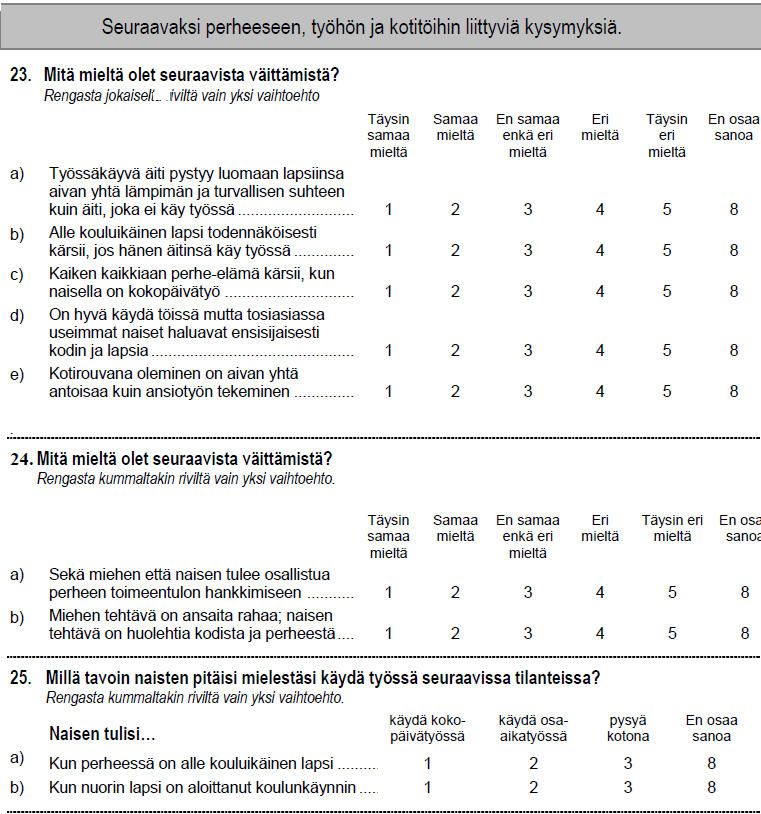
\includegraphics[width=0.5\linewidth]{img/substvar_fi_Q1Q2} 

}

\caption{Suomenkielinen lomake}\label{fig:suom-kys}
\end{figure}

Valituista taustamuuttujista monet on kerätty haastattelulla.
Tiedonkeruu, otantamenetelmät ja yksikkövastauskadon huomioiminen on tehty joka
maassa omalla tavallaan. Aineistoissa on mukana painot joilla tulokset voidaan
korottaa perusjoukon tasolle, mutta kansainvälisiä vertailupainoja ei syystä tai
toisesta ole. Taustamuuttujat kuten koulutustaso on harmonisoitu
vertailukelpoisiksi.

Tutkimuksen kohdeperusjoukko on 18-vuotiaat tai sitä vanhemmat,
poikkeuksina Suomi (15 - 74 vuotiaat), Islanti, Japani, Etelä-Afrikka ja Venezuela.

Jos ohitetaan pienet erot kysymyksissä ja vastausvaihtoehdoissa jäljelle jää
erävastauskato, kyselytutkimusten ominaisuus. Jostain syystä joihinkin kysymyksiin
ei vastata. Esimerkiksi Ranskassa yli 20 prosenttia kieltäytyi vastaamasta lasten
(HHCHILDR) lukumäärää kysyttäessä, ja aika moni myös muissa perherakenteeseen
liittyvissä kysymyksissä. Tässä tutkielmassa monimuuttujakorrespondenssianalyysiä
käytetään tämän ongelman tai datan ominaisuuden analyysiin.

Poistin aineistosta havainnot, joissa tieto iästä tai sukupuolesta puuttuu
(32969-32823 = 146 havaintoa).

Aineiston luokittelu- ja järjestysasteikon muuttujat muunnetaan R-ohjelmiston
factor-tietotyypiksi. Teen muunnokset useammassa vaiheessa heti kun data on
luettu SPSS-tiedosta. Käsittelyssä koitan noudattaa helposti toistettavan
tutkimuksen periaatteita (McNamara ja Horton \citep{RefWorks:doc:5c3759c2e4b0085b307c82b5} ),
koodi ei saisi olla kovin virhealtista (''haurasta'') ja tarkistuksia tehdään
paljon. Data-analyysin ja ehkä erityisesti korrespondenssianalyysin idea on
kuitenkin operoida matriiseilla, lisätä ja poistaa rivejä ja sarakkeita ja
rakennella mutkikkaampia matriiseja yksinkertaisemmista.
Analyysivaiheessa koodi muuttuu hauraammaksi.

\textbf{Aineisto ja korrespondenssianalyysi}

Michael Greenacre on käyttänyt aineistoa eri vuosilta luentomateriaaleissa kuten
Helsingissä 2017\citep{RefWorks:doc:5b6ef091e4b0984fd9b8c0ca} ja ainakin kahdessa
oppikirjassaan(\citep{RefWorks:doc:5a857a43e4b0ed2d44664d7c},
\citep{RefWorks:doc:5a857a43e4b0ed2d44664d78}).
ISSP - aineisto vuodelta 1989 on käytetty myös neljän ``singuaariarvohajoitelmaan
perustuvan menetelmän'' vertailuun\citep{RefWorks:doc:5b6f159ce4b0bc0f31734b76}. Blasius
ja Thiessen (\citep{RefWorks:doc:5b15542ee4b0e2616bc42dca}) arvioivat aineiston laatua
ja ja maiden vertailtavuutta vuoden 1994 aineistolla.

Substanssitutkimusta en käsittele, näiden esimerkkien lisäksi ISSP:n ja
GESIS-instituutin www-palveluista löytyy paljon muitankin.

Sukupuoliroolien (gender roles) ja niihin liittyvien asenteiden vertailevaa
kansainvälistä (cross-cultural) tutkimusta on tehty paljon. Tutkimusongelman
sisällöllisten ja teoreettisen kysymysten nykytilaa kuvaa tuore artikkeli
\citep{RefWorks:doc:5bd08fb6e4b05c5447c9a9f9}.

Toisessa esimerkissä \citep{RefWorks:doc:5bd0a663e4b0c91dcf7c4be9} tutkitaan ensin 18
OECD-maan perhepolitiikan muutoksia kolmen viime vuosikymmenen ajalta. Näkökulma on
työllisyyspolitiikka ja menetelmänä monimuuttuja-korrespondenssianalyysi (MCA).
Havaituille kehityssuunnille etsitään toisessa vaiheessa selityksiä. Aineistona
on viisi kansainväliseen vertailuun soveltuvaa aineistoa, yhtenä niistä ISSP:n
data kolmelta kierrokselta (1988,1994,2002).

\hypertarget{yksinkertainen-korrespondenssianalyysi}{%
\chapter{Yksinkertainen korrespondenssianalyysi}\label{yksinkertainen-korrespondenssianalyysi}}

Korrespondenssianalyysin peruskäsitteet ja muuttujien yhteyden graafisen analyysin
periaatteet voi esittää kahden luokitelumuuttujan ristiintaulukoinnin eli
kontigenssitaulun analyysin avulla. Kyse ei ole pelkästään helposta esimerkistä,
vaan peruskäsitteet ja geometrisiin perusteisiin nojaava graafinen analyysi ovat
oleellisilta osin samat myös monimutkaisemmissa menetelmän sovelluksissa.
MG\&Hastie korostivat tätä, ja MG:n oppikirjat ovat hyvä esimerkki perusteellisesta
yksinkertaisen taulukon analyysin esitystavasta. GDA-kirja (viite) korostaa
ranskalaisen perinteen mukaisesti matemaattista teoriaperustaa, mutta myös siinä
menetelmä peruskäsitteet ja tulkinnat esitellään yksinkertaisella esimerkillä
(Fisherin Cairness-data, Mustonen (viite) käyttää samaa dataa).

Esitän tässä jaksossa korrespondenssianalyysin peruskäsitteet intuitiivisesti,
matemaattiset yksityiskohdat löytyvät liittestä 1. Esitystavan etu on taulukon
pieni koko, johtopäätökset voi helposti tarkastaa datasta.
Näin päästään nopeasti pääasiaan, graafiseen analyysiin.

Tämä ei ole ainoa mahdollinen näkökulma, korrespondenssianalyysillä on useita
vaihtoehtoisia tulkintoja. Se voidaan ymmärtää myös moniulotteisen
varianssianalyysin kaltaiseksi hajonnan dekomponoinnin menetelmäksi.
GDA-kirjassa numeeriset tulokset ovat tulkinnan lähtökohtana ja vasta sitten
katsotaan graafista esitystä. CAiP (viite) pitää numeerisia tuloksia tärkeinä,
niiden avulla varmistetaan kuvan tulkinnan pätevyys.

\hypertarget{uxe4iti-tuxf6issuxe4---kuxe4rsiikuxf6-lapsi}{%
\section{Äiti töissä - kärsiikö lapsi?}\label{uxe4iti-tuxf6issuxe4---kuxe4rsiikuxf6-lapsi}}

Aineisto on kuuden maan vastaukset kysymykseen Q1b: ''Alle kouluikäinen lapsi
todennäköisesti kärsii, jos hänen äitinsä käy työssä''. Kysymys on voimakkaasti
muotoiltu (\textbf{edit}MG on jossain jutussa havainnut, että kyselyn kahdessa
kysymyksessä on sana ''äiti'' ja niiden vastausten jakaumat poikkeavat. Jos löydän
lähteen lisään sen tähän). Kysymykset on suunniteltu kokonaisuudeksi, ja niitä
analysoidaan yhdessä luvussa 7, yhden taulukon analyysi esittelee menetelmän.
(alaviite:Tämän havaitsi eräs lastensuojelun ammattilainen: kysymys on
irrallisena monimerkityksellinen (vähintään ns. ''double - barreled''), eikä
siihen voi oikein järjevästi vastata. Pitäisi tietää missä lapsi on, mitä hän
tekee). Havainnot joissa tieto vastauksesta puuttuu on poistettu aineistosta.
Taustamuuttujia ovat vastaajan sukupuoli ja ikä.

Frekvenssitaulukossa \ref{tab:simpeCA-frekTa1} on esitetty vastausten suhteellinen jakauma,
lukumäärät on jaettu havaintojen lukumäärällä (8143). Korrespondenssianalyysissä
kaikki on suhteellista, ja analyysi perustuu tähän taulukkoon. Taulukon
reunajakaumat kertovat jokaisen maan ja jokaisen vastausvaihtoehdon suhteellisen
osuuden. Näitä suhteellisia osuuksia kutsustaan korrespondenssianalyysissä
\emph{rivi- ja sarakemassoiksi}.

\begin{table}

\caption{\label{tab:simpeCA-frekTa1}Kysymyksen Q1b vastaukset maittain, suhteelliset frekvenssit}
\centering
\begin{tabular}[t]{lllllll}
\toprule
  & S & s & ? & e & E & Total\\
\midrule
BE & 2.35 & 5.54 & 5.38 & 6.78 & 4.68 & 24.72\\
BG & 1.45 & 4.85 & 2.52 & 2.33 & 0.16 & 11.31\\
DE & 2.03 & 4.61 & 2.43 & 6.61 & 5.38 & 21.05\\
DK & 0.86 & 2.92 & 1.87 & 2.85 & 8.55 & 17.05\\
FI & 0.58 & 2.31 & 1.83 & 5.19 & 3.72 & 13.63\\
\addlinespace
HU & 2.69 & 3.54 & 2.76 & 2.33 & 0.92 & 12.24\\
Total & 9.95 & 23.76 & 16.79 & 26.10 & 23.41 & 100.00\\
\bottomrule
\end{tabular}
\end{table}

Muuttujien luonne on usein erilainen. Tähän aineistoon sopii
riviprosenttientaulukko, vertaillaan vastausten jakaumia maiden välillä. Taulukon
sarakkeet ovat muuttujia ja rivit havaintoja. Rivit on saatu summaamalla
(aggregoimalla) vastaukset maittain.
(viite: MG kutsuu näitä rivejä termillä samples, osajoukot).

\begin{table}

\caption{\label{tab:simpeCA-rprosTa1}Kysymyksen Q1b vastaukset, riviprosentit}
\centering
\begin{tabular}[t]{lllllll}
\toprule
  & S & s & ? & e & E & Total\\
\midrule
BE & 9.49 & 22.40 & 21.76 & 27.42 & 18.93 & 100.00\\
BG & 12.81 & 42.89 & 22.26 & 20.63 & 1.41 & 100.00\\
DE & 9.63 & 21.88 & 11.55 & 31.39 & 25.55 & 100.00\\
DK & 5.04 & 17.15 & 10.95 & 16.71 & 50.14 & 100.00\\
FI & 4.23 & 16.94 & 13.42 & 38.11 & 27.30 & 100.00\\
\addlinespace
HU & 21.97 & 28.89 & 22.57 & 19.06 & 7.52 & 100.00\\
All & 9.95 & 23.76 & 16.79 & 26.10 & 23.41 & 100.00\\
\bottomrule
\end{tabular}
\end{table}

Sarakeprosentit antavat toisen näkökulmaan samaan dataan.

\begin{table}

\caption{\label{tab:simpeCA-cprosTa1}Kysymyksen Q1b vastaukset, sarakeprosentit}
\centering
\begin{tabular}[t]{lllllll}
\toprule
  & S & s & ? & e & E & All\\
\midrule
BE & 23.58 & 23.31 & 32.04 & 25.98 & 19.99 & 24.72\\
BG & 14.57 & 20.41 & 15.00 & 8.94 & 0.68 & 11.31\\
DE & 20.37 & 19.38 & 14.48 & 25.32 & 22.98 & 21.05\\
DK & 8.64 & 12.30 & 11.12 & 10.92 & 36.52 & 17.05\\
FI & 5.80 & 9.72 & 10.90 & 19.91 & 15.90 & 13.63\\
\addlinespace
HU & 27.04 & 14.88 & 16.46 & 8.94 & 3.93 & 12.24\\
Total & 100.00 & 100.00 & 100.00 & 100.00 & 100.00 & 100.00\\
\bottomrule
\end{tabular}
\end{table}

Tavoitteena on korrespondenssianalyysin kartta, jossa rivi- ja sarakepisteet on
esitetty samassa kuvassa. Sarakeprosenttien taulukossa on esitetty sarakkeiden
suhteelliset jakaumat. Näitä suhteellisia rivejä ja sarakkeita kutsutaan
korrespondenssianalyysissä \emph{rivi- ja sarakeprofiileiksi}.

\textbf{k} Rivit on saatu alkuperäisestä aineistosta osajoukkojen summina. MG:n
terminologialla ``samples''.

Korrespondenssianalyysin perusidea on analysoida rivien ja sarakkeiden yhteyttä
(korrespondenssia) rivi- tai sarakeprofiilien hajonnan avulla. Hajontaa mitataan
poikkeamilla keskiarvorivistä tai sarakkeesta, ja massat otetaan huomioon,
kun hajonnat lasketaan yhteen.

\begin{figure}
\centering
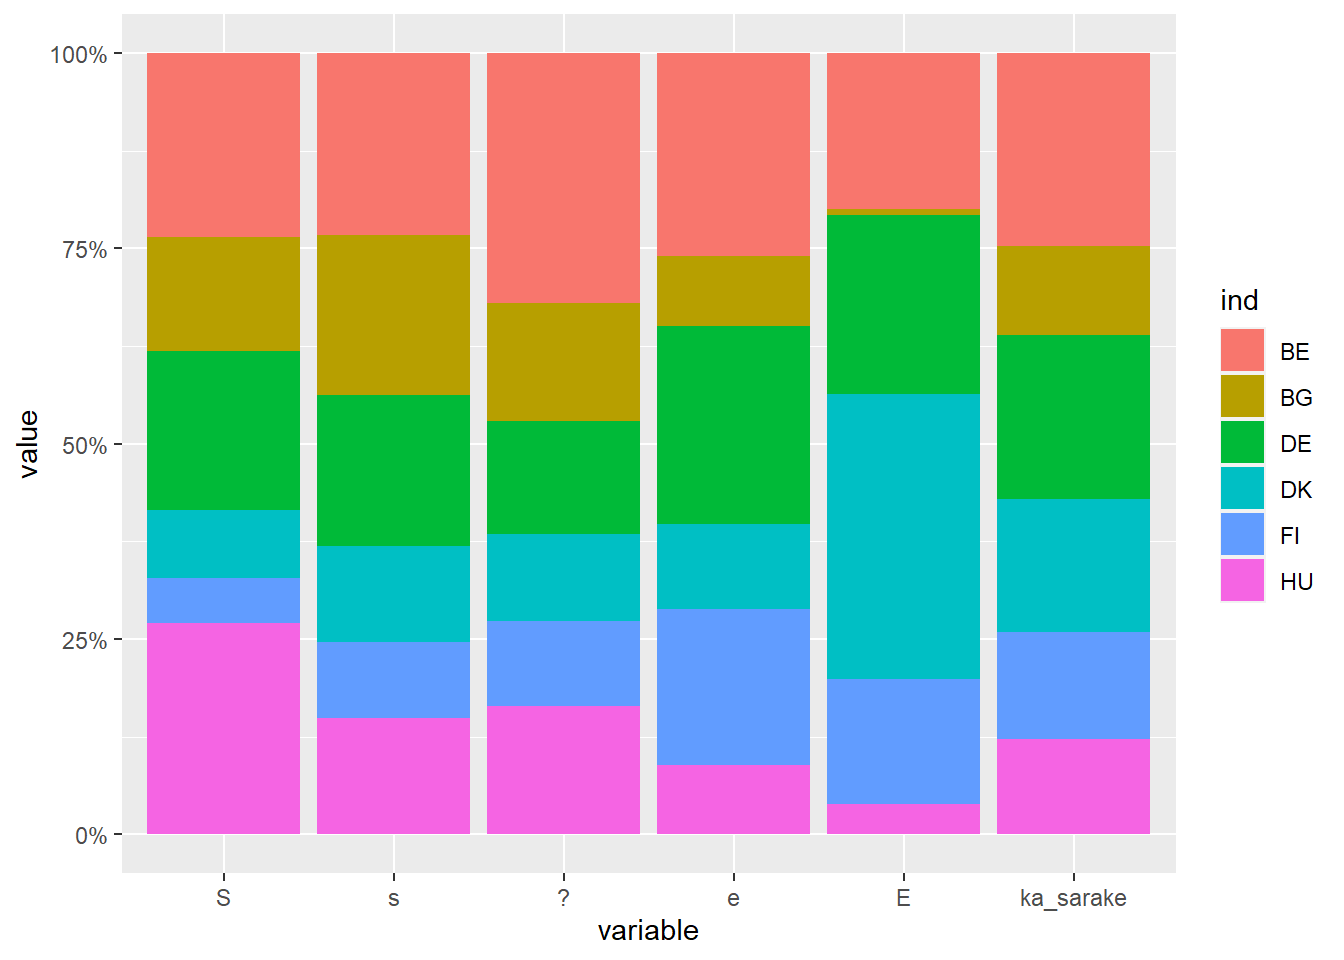
\includegraphics{JH_capaper_files/figure-latex/g1-2kuva1-1.pdf}
\caption{\label{fig:g1-2kuva1}Q1b:Sarakeprofiilit ja keskiarvoprofiili}
\end{figure}

\begin{figure}
\centering
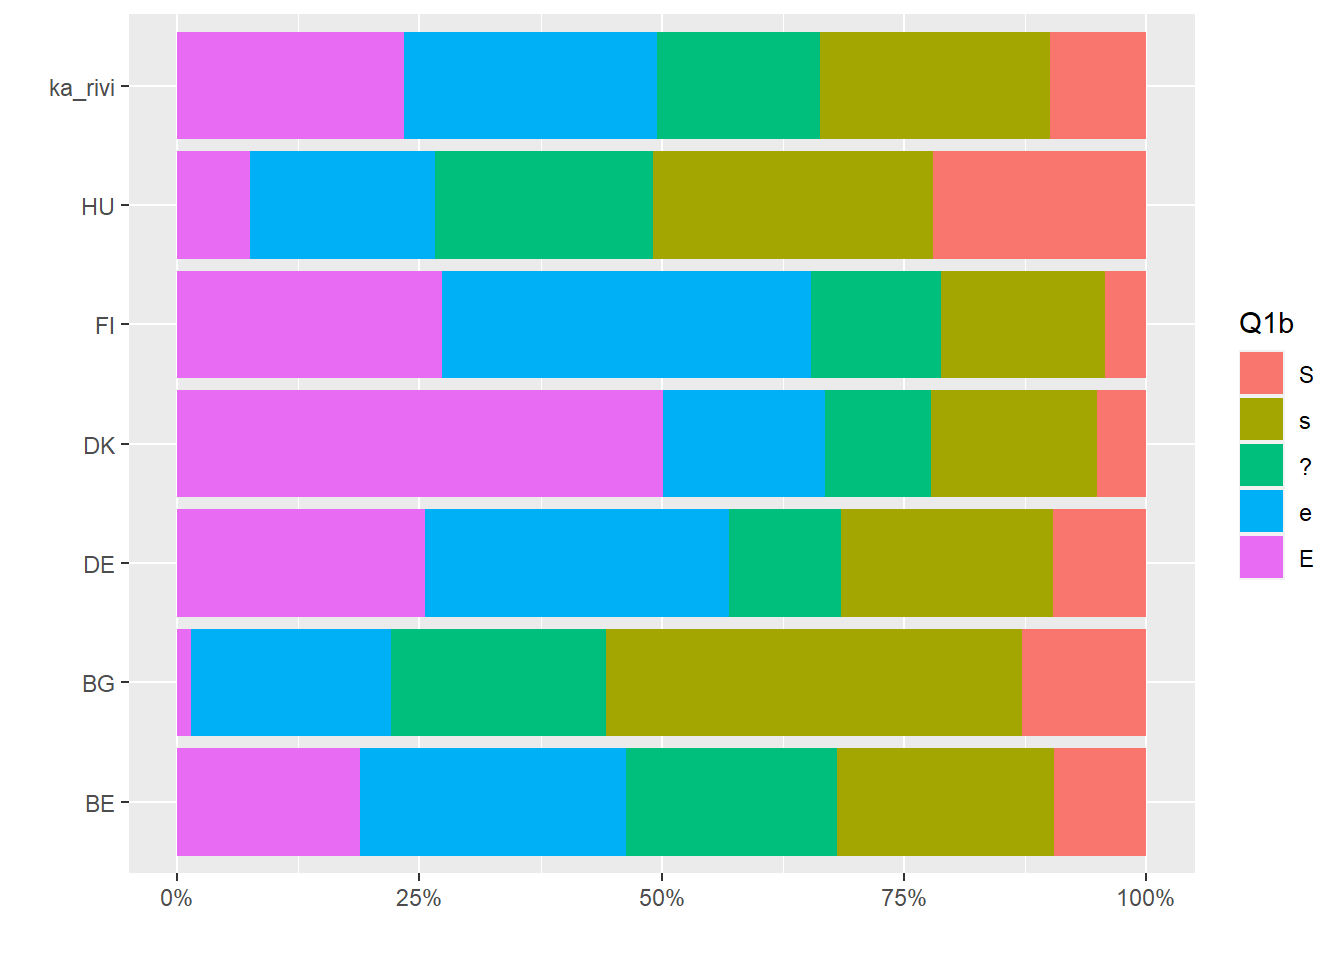
\includegraphics{JH_capaper_files/figure-latex/g1-2kuva2-1.pdf}
\caption{\label{fig:g1-2kuva2}Q1b: riviprofiilit ja keskiarvorivi}
\end{figure}

Kuvasta 3.2 \ref{fig:g1-2kuva2} esimerkiksi näkee, että Tanska (DK) näyttäisi
poikkeava keskiarvorivistä paljon, samoin Bulgaria.
Bulgarian massa on kuitenkin aineiston pienin (11,31 \%), Tanskan taas
kohtalainen (17 \%).
Sarakeprofiilikuvassa \ref{fig:g1-2kuva1} täysin eri mieltä - vastaus (E) on
selvästi erilainen ja sen massa on suuri (23\%). Kaikki luvut ovat suhteellisia,
havaintojen lukumäärä ei vaikuta tulkintaan periaatteessa mitenkään.

Mikä on rivien (havaintojen) ja sarakkeiden (muuttujien) yhteys?

Kahden luokittelumuuttujan riippuvuutta voidaan testata \(\chi^{2}\) - testillä.
Riippumattomuushypoteesin mukainen odotettu solufrekvenssi on taulukon
\ref{tab:simpeCA-frekTa1} reunajakaumien alkioiden tulo.

Testisuure saadaan laskemalla yhten jokaisen solun havaittujen ja odotetettujen
frekvenssien erotukset muodossa

\begin{equation}
  \chi^{2} = \frac{(havaittu - odotettu)^2} {odotettu}
    \label{eq:khii21}
\end{equation}

Tämä voidaan esittää ca:han sopivammalla tavalla parilla muunnoksella, jolloin
saamme riveittäin vastaavat termit rivisummalla painotettuna:

\begin{equation}
  rivisumma \times \frac{(havaittu \: riviprofiili - odotettu \: riviprofiili)^2} {odotettu \: riviprofiili}
    \label{eq:khii22}
\end{equation}

Kun jaamme nämä tekijät havaintojen kokonaismäärällä \(n\), rivisumma muuntuu
rivin massaksi, ja niiden summa muotoon \(\frac{\chi^{2}}{n}\).

\begin{equation}
 \frac{\chi^{2}}{n} = \phi^{2}
  \label{eq:inert1}
 \end{equation}

Jakajassa ei ole vapausastekorjausta (n-1), korrespondenssianalyysi on
deskriptiivistä data-analyysiä.

Tunnusluku \(\phi^{2}\) on korrespondenssianalyysissä kokonaisinertia (total
inertia). Se kuvaa, kuinka paljon varianssia taulukossa on ja on riippumaton
havaintojen lukumäärästä. Tilastotieteessä tunnusluvulla on useita vaihtoehtoisia
nimiä (esim. mean square contingency coefficient), ja sen neliöjuurta kutsutaan
\(\phi\) - kertoimeksi.

Korrespondenssianalyysin algoritmit operoivat suhteellisten frekvenssien
taulukkolla. Kaavojen \eqref{eq:khii21} ja \eqref{eq:khii22} yhteyden pitäisi olla
selkeä.

Frekvenssitaulukossa (jossa kaikki taulukon luvut on jaettu havaintojen
lukumäärällä N riviprofiilien 1 ja 3 (euklidinen) etäisyys on

\begin{equation}
 \sqrt{(p_{11} - p_{31})^2 + (p_{12} - p_{32})^2 + (p_{13} - _{33})^2+ (p_{14} - _{34})^2+ (p_{15} - _{35})^2}
 \label{eq:euclid1}
 \end{equation}

Rivien \(\chi^{2}\) - etäisyys on painotettueuklidinen etäisyys, jossa painoina
ovat riviprofiilin odotetut arvot. Ne ovat riippumattomuushypoteesin mukaisesti
riviprofiilien keskiarvoprofiilin vastaavat alkioit \(r_{i}\) .

\begin{equation}
 \sqrt{\frac{(p_{11} - p_{31})^2} { r_{1}} + \dots + \frac{(p_{15} - p_{35})^2} {r_{5}}}
 \label{eq:euclid2}
\end{equation}

Inertia voidaa esittää rivien ja keskiarvorivin (sentroidin) \(\chi^{2}\) -etäisyyksien
neliöiden painotettuna summana, jossa painoina ovat rivien massat \(m_{i}\) ja
summa lasketaan yli rivien \({i}\).

\begin{equation}
 \phi^{2} = \sum_{i} (massa \: m_{i}) \times (profiilin \: i \: \chi^{2} - etaisyys \: sentroidista)^{2}
 \label{eq:inert2}
\end{equation}

\textbf{edit} Tässä esitystavassa viite on CAiP, teorialiitteessä tarkemmin. Tarkoitus on esittää
yksinkertaisesti taulukon datan analyysin käsitteet ja CA:n peruskäsitteet profiili,
massa ja \(\chi^{2}\) - etäisyys

Rivi- ja sarakeprofiilien taulukoista näkee helposti, että keskiarvoprofiilien
alkiot ovat massoja. Rivien keskiarvoprofiilin alkiot ovat sarakemassoja, ja sama
pätee sarakkeille. Tämä rivi- ja sarakeongelmien duaalisuus on yksinkertaisen
korrespondenssianalyysin keskeinen idea. Greenacren perusoppikirjassa ensimmäiset
luvut esittelevät lähes kaikki menetelmän perusideat eri näkökulmilla
tällaiseen taulukkoon (CAiP).

\textbf{k} ca-ratkaisu: rivi- ja sarekepilvien dimensio on sarakkeiden tai rivien
lukumäärä vähennettynä yhdellä, pienempi kahdesta vaihtoehdosta. Tämä seuraa
yksikertaisesti rivi- ja sarakeprofiilien suhteellisuudesta, niiden summat ovat 1.

\textbf{k} Etsitään kaksiulotteinen ratkaisu (taso), joka minimoi pisteiden
khii2-etäisyyksien poikkeamien summan eli on mahdollisimman lähellä pisteitä.

\textbf{K} rivi- ja sarakeongelma ratkaisu johtaa saamaan lopputulokseen. Tämä
duaalisuus on korrespondenssianalyysin perusominaisuuksia.

\hypertarget{korrespondenssianalyysin-esimerkki-symmetrinen-kartta}{%
\section{Korrespondenssianalyysin esimerkki: symmetrinen kartta}\label{korrespondenssianalyysin-esimerkki-symmetrinen-kartta}}

\begin{figure}

{\centering 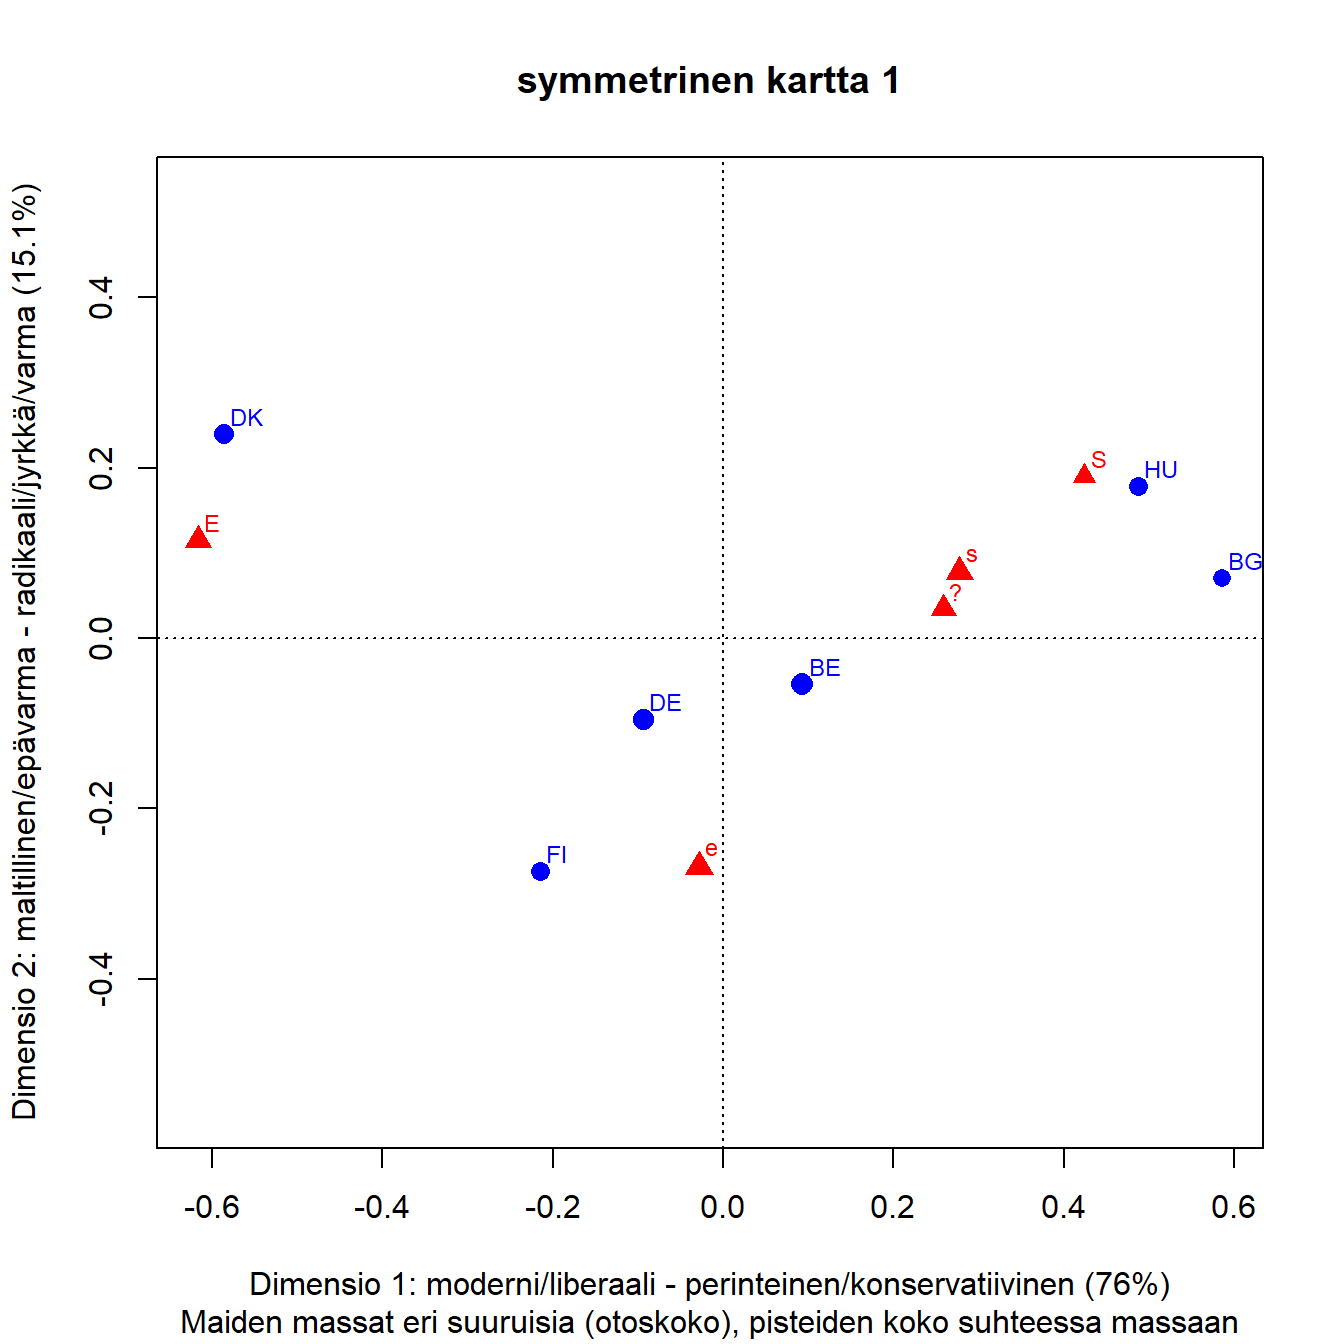
\includegraphics[width=0.9\linewidth]{JH_capaper_files/figure-latex/simpleCA1map1-1} 

}

\caption{Q1b: lapsi kärsii jos äiti on töissä}\label{fig:simpleCA1map1}
\end{figure}

Kartassa (symmetrisessä kartassa) on jo nimetty molemmat akselit, mutta tulkinta
aloitetaan prosenteista. Ne kertovat, kuinka paljon aineiston inertiasta eli
hajonnasta on kaksiulotteisesssa projektiossa saatu kuvattua akseleille.

Ensimmäinen akseli saa aina suurimman osan inertiasta, tässä 76 prosenttia.
Kun toinen akseli kuvaa 15 prosenttia koko inertiasta, on kartalla esitetty 91
prosenttia aineiston hajonnasta. Loput 9 prosenttia jää 3. ja 4. dimensiolle.
Nämä ''selitysosuudet'' ovat samantapainen laskelma kuin perinteisen regressiomallin
''selitetty'' vaihtelu ja ''jäännösvaihtelu''.

\emph{Kontrastit} määrittävät akselien tulkinnan . Benzacrin ohjeen mukaan (1992,
teoksessa GDA s. 49) katsotaan mitä on oikealla ja mitä vasemmalla. Akselien
tulkinta perustuu siihen, mitä mitä yhteistä on kaikilla elementeillä jotka ovat
origon vasemmalla puolella ja vastaavasti origon oikealla puolella. Samalla tavalla
tulkitaan toinen akseli, mitä on ylhäällä ja alhaalla.

\textbf{edit}Käytän jatkossa muuttujista niiden symboleja sanallisen kuvauksen sijaan.

Tässä tapauksessa taulukon rivit ovat havaintoja (''samples'' ) ja sarakkeet
muuttujia, ja akselien tulkinta tehdään muuttujien avulla. Vasemmalla on E ja
oikealla puolella samanmieliset vastaukset s ja S. Neutraali ''?'' on s-vastausten
vasemmalla puolella. Kun erot ovat suhteellisia, ei kuvan perusteella voi sanoa
kuinka paljon.

Sarakkeet voi projisoida ensimmäiselle akselille (ts. katsoa niiden x-koordinaatin)
, ja tässä ne ovat ``oikeassa järjestyksessä''.
Jos vastausvaihtoehdoille haluaisi antaa numeeriset arvot, x-akselin koordinaatti
olisi ehkä parempi kun järjestysnumero?

Ensimmäisen dimenosion tulkinta on aika selkeä. Toinen akseli on kontrasti
lievemmän tai maltillisemman erimielisyyden ja muiden vastausten kanssa.
Se on 1. dimension suuntaan kaikkein lähimpänä origoa. Hieman varoivaisemmin
akselin voi tulkita maltillisen ja jyrkemmän tai varmemman mielipiteen kontrastiksi.

Maiden vertailu tehdään näiden akselien suuntaan. Sekä sarekepisteiden että
rivipisteiden keskinäiset välimatkat approksimoivat optimaalisesti niiden
(khii2)etäisyyksiä. Sarake- ja rivipisteiden välisillä etäisyyksillä ei ole
mitään suoraa tulkintaa. Pisteiden etäisyydet samassa pistepilvessä ovat
suhteellisia, Saksa on konsevatiivisempi kuin Suomi mutta emme tiedä kuinka paljon.
Maiden järjestys oikealta vasemmalle on selkeä, Tanska on vasemmalla
liberaalina ''ääripäänä'', oikealla taas Unkari ja Bulgaria. Pystyakselin suuntaan
nähdään, että kaikkein ''maltillisin'' mutta kuitenkin liberaali on Suomi,
jyrkimmät mielipiteet löytyvät Unkarista ja Tanskasta.

Näitä tulkintoja voi vertailla edellä esitettyihin kahteen kuvaan rivi- ja
sarakeprofiileista. Kartta kertoo aika paljon enemmän.
Kartta on approksimaatio neliulotteisen pistepilven hajonnalle. Vain origo on
siinä tarkasti esitetty, se on koko aineiston keskiarvopiste, ja pisteiden
hajonta sen ympärillä kuvaa poikkeamaa riippumattomuushypoteesista.

Tärkeä geometrinen periaate on se, että kaukana on kaukana myös alkuperäisessä
pistepilvessä, mutta kartalla lähellä olevat pisteet eivät välttämättä ole lähellä.
Projektio kutistaa pisteiden etäisyyksiä.

Approksimaation laatu selviää korrespondenssianalyysin numeerisista tuloksista,
samoin se miten rivi- ja sarakepisteen määrittävät akselit.

Kartoissa tärkein tekninen yksityiskohta on kuva- tai muotosuhde (aspect ratio).
Akseleiden mittayksikön pitää olla sama eli muotosuhteen yksi. Jos kuvia
tulostetaan useassa formaatissa kannattaa olla tarkkana. Kuvien on jo
analyysivaiheessa oltava lukukelpoisia, ja symbolien kokoa joutuu isoissa
aineistoissa säätämään. Tulosten esittäminen lopullisessa muodossa vaatii jo
paljon vaivannäköä, tässä tutkielmassa esitetään vain datan analysoinnin
valikoituja kuvia. Graafinen data-analyysi on vaivatonta vasta sitten kun se tehty.
En jatkossa esitä kuvailevia akseleiden nimiä kuvissa,
akseleiden nimeäminen on kuvan tulkinnan toinen askel.

Liitteessä 1 on esitetty korrespondenssianalyysin matemaattisen ratkaisun periaate.

\textbf{k} Kuva tai kartta - käytän termejä synonyymeinä - on se taso, joka parhaiten
''selittää'' neliulotteisen pisteparven hajontaa suhteessa koko aineiston
keskiarvopisteeseen eli sentroidiin. Matemaattisesti ratkaisu saadaan
soveltamalla singulaariarvohajoitelmaa, ja tulokseksi saadaa taso joka on
lähimpänä pistepilviä. Etäisyyttä mitataan massoilla painotetulla
khii2-etäisyysmitalla.

\textbf{k} Intuitiivisesti idea on aivan sama kuin pääkomponenttianalyysissä
(PCA, principal component analysis). Ratkaisu löydetään akseli kerrallaan.
Ensi pistepilvestä etsitää akseli, jolle ortogonaalisesti projisoitujen
pisteiden hajonta on suurin. Sitten etsitään sille kohtisuora toinen akseli
samalla säännöllä, ja näin jatketaan kunnes koko pilven hajota on jaettu näille
uusille akseleille. tavoitteena on muutaman dimension approksimaatio
moniulotteiselle datalle, yleensä kaksiulottoinen kartta.

\textbf{k} CA on paintotettu PCA

\hypertarget{korrespondenssianalyysin-peruskuxe4sitteet}{%
\section{Korrespondenssianalyysin peruskäsitteet}\label{korrespondenssianalyysin-peruskuxe4sitteet}}

\textbf{edit} Sulava kuvaus tulkinnasta, painotus kuvien tulkinnassa. CA:n numeeriset
tulokset vasta seuraavassa luvussa. Tässä ``mitä kuvasta näkee'', ei muuta (paitsi
varoitukset - mitä ei näe). Idea koko ajan taulukon sarakkeiden ja riveien yhteyksien
visualisointi.

\textbf{edit} Tärkeää selkeä kuvaus pääkoordinaattien ja standardikoordinaattien
suhteesta. Tarkemmin teorialiitteessä, tässä heuristisesti jotta kuvia osaa tulkita.

Korrespondenssianalyysille on vakiintunut oma käsitteistö, joista tärkeimmät on
jo mainittu. Kun tulkinta perustuu ''ääripäihin'', puhutaan kontrasteista ja
distinktiosta. Luokittelumuuttujan arvot taas ovat modaliteetteja.
Tärkein periaate on se, että kaikki on suhteellista. Ydinkäsitteitä ovat
\emph{korrespondenssianalyysin ''tripletti'': khii2-etäisyys, massat ja profiilit}.

Kolmikkoa täydentää ''kvartetti'', neljä siitä johdettua käsitettä: \emph{inertia} eli
(painotettu) varianssi, \emph{sentroidi} (painotettu keskiarvo, barysentrinen periaate),
\emph{aliavaruus} ja \emph{projektio}. (CAiP, s. 49).

\emph{k} rivi- ja sarakeratkaisun duaalisuus: viite CAiP, jossa käydään läpi
perusteellisesti. Rivi- ja sarakeratkaisut liittyvät tiivisti toisiinsa, kts.
teorialiite.

\emph{k} khii2-etäisyys on profiilien painotettu euklidinen etäisyys (ja toki
neliöjuuri!) jossa painoina ovat keskiarvoprofiilin elementtien käänteisluvut
eli elementtien etäisyyden neliö jaetaan keskiarvoprofiilin alkiolla.

\textbf{edit}: khii2-etäisyydestä ehkä teorialiitteeseen?

\emph{k} khii2-testin oletukset eivät välttämättä ole voimassa kaikissa aineistoissa,
mutta etäisyysmittaa käytetään silti, sen perustelu on paljon yleisempi.

\emph{k} khii2-etäisyys on ainoa etäisyysmitta, joka toteuttaa distributional
equivalence - periaatteen, CA:n ''tärkein juttu'' (Benzecri), avain kaikkiin CA:n
ominaisuuksiin. (Viite:CAip epilogi)

\emph{k} normalisointi, samaan tapaan kuin PCA:ssa. Jos lukumäärätaulukko,
Poisson-jakauman hajonta on sama kuin odotusarvo eli jaetaan poikkeama
keskiarvosta hajonnalla. Poisson-jakaumassa odostusarvo ja hajonta ovat sama
parametri. Tämä tulkinta khii2-etäisyydelle ei kuitenkaan saisi hämärtää massojen
kaksoisroolia: ne ovat profiilien painoja ja samalla standardoivat khii2-etäisyyden.

\emph{k} CAiP epilogi: khii2 on yhteys Mahlanobis-etäisyyteen ja multinomijakaumaan,
jonka realisaatioiksi profiilit voidaan tulkita. (s. 301).

\textbf{Millaista dataa?}

Korrespondenssianalyysin sovelletaan yleisimmin frekvenssitaulujen analyysiin,
lukumäärädataan (count data). Periaatteessa mikä tahansa data sopii, kunhan se
voidaan järkevästi esittää suhteelisina lukumäärinä (relative amounts), siis
suhdeasteikon (ratio scale) muuttujana. Tässä oleellista on tulkittavuus
tutkimusongelman näkökulmasta. Välttämätön ehto on sama mittayksikkö: lukumäärä,
rahayksikkö, pituusmitta kelpaavat. (CAiP s. 15).
Toinen ehto on ei-negatiivisuus (nolla tai nollaa suurempi luku) ,
kts. kuitenkin GDA (tietyilllä ehdoilla myös neg. arvot. Rajat ovat melko
joustavat, kun mukaan otetaan erilaiset uudelleenskaalaukset ja transformaatiot.
Tämä oli menetelmän perusidea jo Benzecrillä(CAiP ch 26, s. 201).

Menetelmää sovelletaan profiileihin jotka painotetaan massoilla, ja
profiilien etäisyyksiä mitataan khii2-etäisyysmitalla. Jos datan voi esittää
tässä muodossa, menetelmää voi käyttää.

\hypertarget{asymmetrinen-kartta-ja-ideaalipisteet}{%
\subsection{Asymmetrinen kartta ja ideaalipisteet}\label{asymmetrinen-kartta-ja-ideaalipisteet}}

Symmetrinen kartta \ref{fig:simpleCA1map1} on peruskuva ja esimerkiksi tässä
käytetyn R-paketin ``ca'' oletus. Siinä molemmat pisteparvet on esitetty
pääkoordinaateissa (prinipal coordinates) ikäänkuin päällekkäin, samassa kuvassa.

Toinen vaihtoehto on asymmetrinen kartta. Sarakkeet ovat aineistossa muuttujia,
joten ne voi esittää ns. standardikoordinaateissa ja rivipisteet pääkoordinaateissa.

Sarakepisteitä kutsutaan ideaalipisteiksi, ne edustavat kuviteellisia maita joissa
kaikki vastaukset ovat samoja. Matemaattisesti kartalle projisoidut ideaalipisteet
ovat (tässä esimerkissä) neliulotteisen avaruuden verteksin (monikulmion)
kärkipisteitä. Rivipisteet ovat tämän verteksin sisällä.

\begin{figure}

{\centering 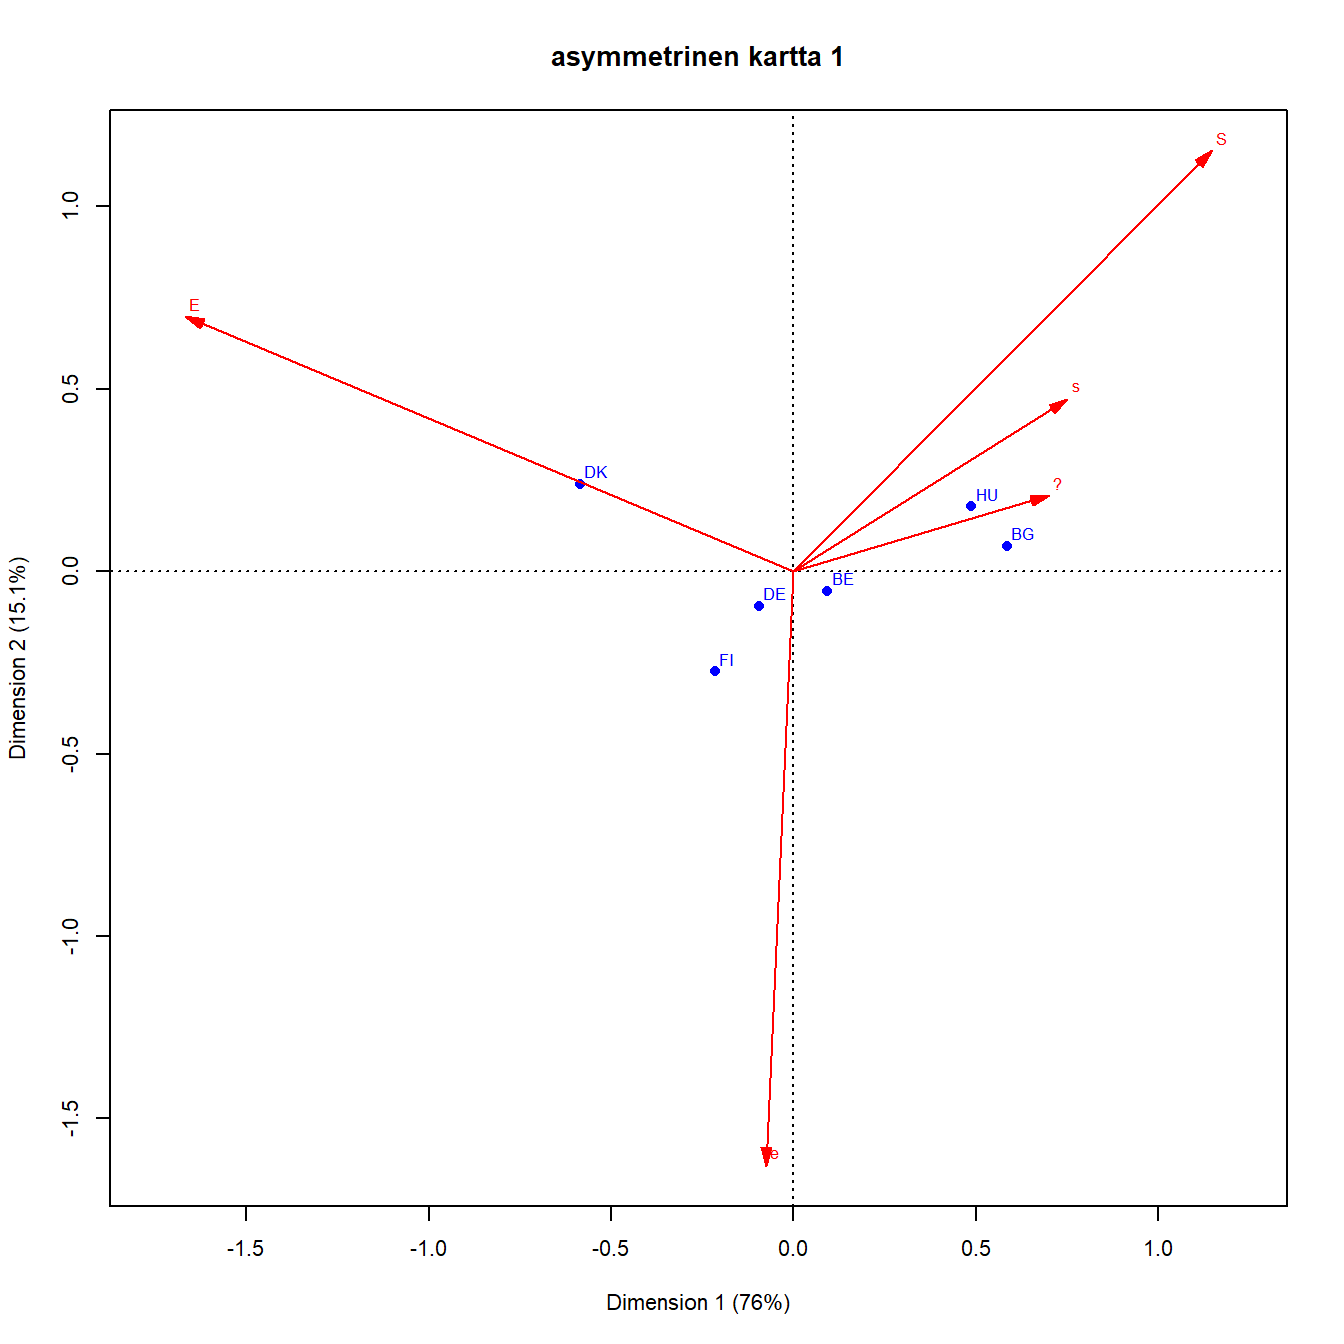
\includegraphics[width=0.9\linewidth]{JH_capaper_files/figure-latex/G1-3asymm2-1} 

}

\caption{Q1b: lapsi kärsii jos äiti on töissä}\label{fig:G1-3asymm2}
\end{figure}

Sarakepisteet kuvaavat maksimi-inertiaa, ja rivipisteiden paljon pienempi hajonta
kuvaa niiden poikkeamaa tästä hypoteettisesta tilanteesta. Sarakepisteet
skaalautuvat origosta ulospäin, Asymmetrisessä kartassa rivi- ja sarakepisteiden
etäisyydellä on tulkinta, samoin rivipisteiden välisellä etäisyydellä.
Sarakepisteiden välisillä etäisyyksillä ei ole tulkintaa. Sarakepisteet on
skaalattu ja mittakaavan ero symmetriseen karttaan näkyy selvästi.

\textbf{Barysentrinen periaate}

Rivipisteet ja sarakepisteet yhdistää \emph{barysentrinen\_periaate} . Jokainen rivipiste
on ideaalipisteiden painotettu keskiarvo, painoina sarakkeiden käänteinen osuus
riviprofiilissa.

\textbf{edit} kuva ei ehkä tarpeen? Tehdään vähän pienempi (out.width = 60\%, muuten 90\%).

\begin{figure}

{\centering 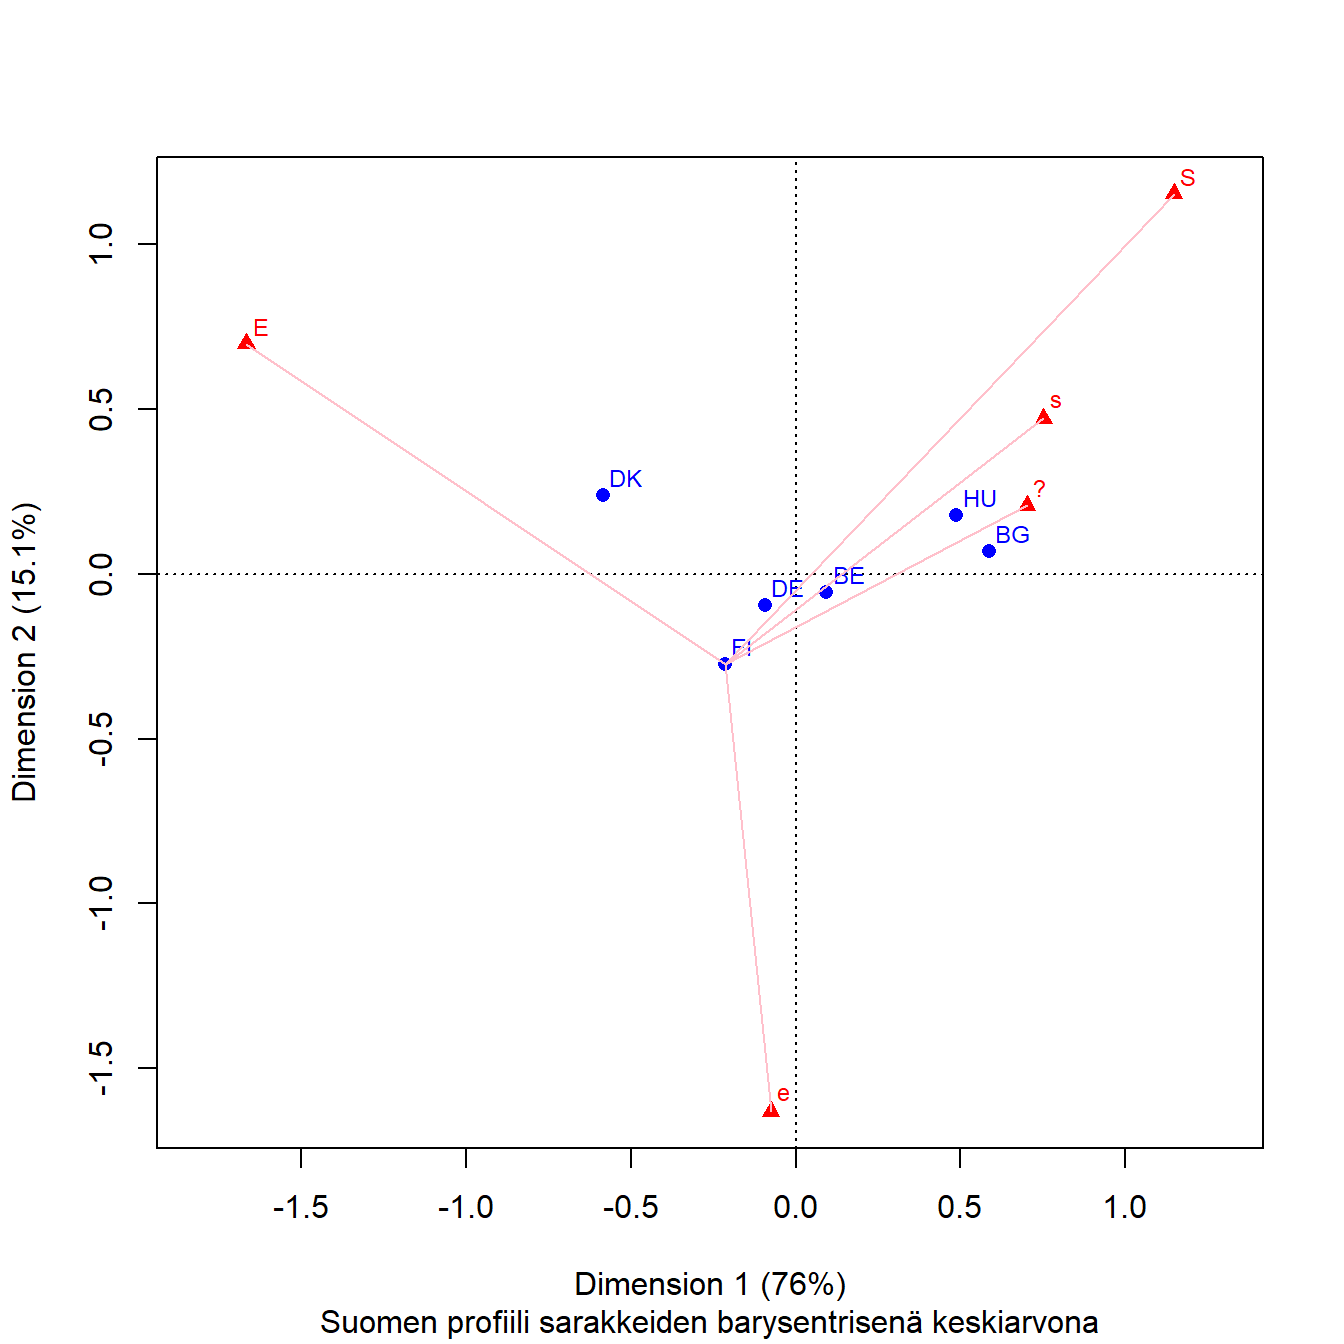
\includegraphics[width=0.7\linewidth]{JH_capaper_files/figure-latex/G1-3asymm3-1} 

}

\caption{Q1b: lapsi kärsii jos äiti on töissä}\label{fig:G1-3asymm3}
\end{figure}

Suomen profiili on kaukana S-sarakkeesta ja lähellä ? - saraketta, niiden osuus
profiilissa on suuri.

Ideaalipisteiden tulkinnan voi varmistaa sarake kerrallaan, projisjoimalla rivipisteet
origon kautta piirretylle janalle. Kuvassa @ref(fig:G1\_3\_asymmtulk2) nähdään mikä
on maiden järjestys E-vastausvaihtoehdossa.

\begin{center}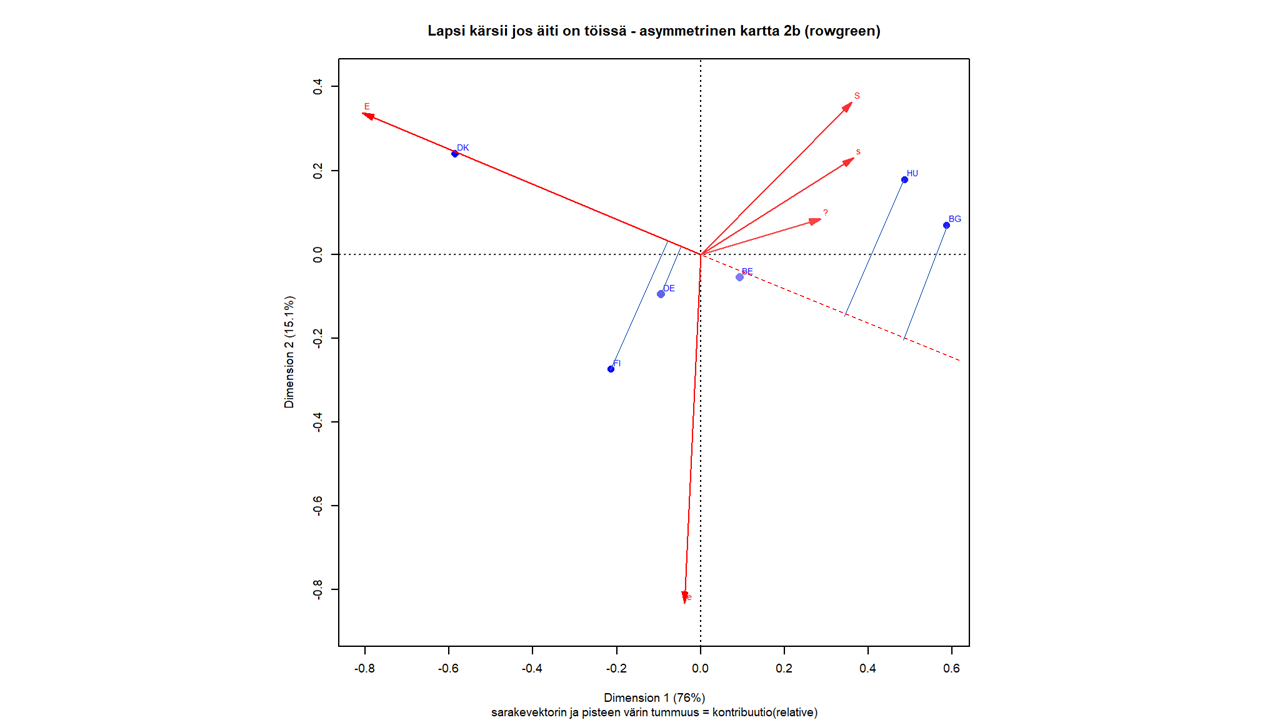
\includegraphics[width=0.9\linewidth]{img/simpleCAasymmTulk2} \end{center}

Asymmetrinen kartta antaa kaksi uutta näkökulmaa rivien ja sarakkeiden suhteeseen.
Sen huono puoli on ideaalipisteiden karkaaminen kauas origosta ja rivipisteiden
pakkautuminen pieneksi parveksi. Jos rivipisteiden hajonta on suuri,
kuva on käytännöllinen. Kyselytutkimusaineistoissa näin ei yleensä ole.

\hypertarget{kontribuutiot-kartalla}{%
\section{Kontribuutiot kartalla}\label{kontribuutiot-kartalla}}

Analyyseissä käytetty r-paketti ``ca'' esittää kartoilla myös pisteiden massat pisteen
symbolin kokona, mutta tässä aineistossa eroja on vaikea nähdä. Tärkeämpi on pisteiden
\emph{kontribuutioiden} esittämien värisävynä.

Kun kartalla pistejoukon inertia kuvataan akseleille, on jokaisella pisteellä oma
osuutensa akseleiden kuvaamasta inertiasta. Absoluuttinen kontribuutio kertoo rivin
tai sarakkeen osuuden akselin inertiasta. Vaikutuksessa on mukana pisteen massa.

Suhteellinen kontribuutio taas kertoo akselin osuuden pisteen inertiasta.
Tämä tunnusluku kuvaa pisteen projektion laatua, kuinka hyvin se on kartalla esitetty.

Kontribuutiokartta on asymmetrinen kartta, jossa sarakevektorit on skaalattu
(kerrottu) massojen neliöillä. Näin sarakevektorit ``kutistuvat'' kohti origoa mutta
vektorin pituus kertoo edelleen sen suhteellisen massan. Kartta sopii niin pienen
kuin suuren inertian tilanteisiin(kts. esim. \citep{RefWorks:doc:5c768b09e4b02df9431e950a})

\textbf{Absoluuttiset kontribuutiot}

Absoluuttisten kontribuutioiden jakautumista akseleille voi varovaisesti päätellä
sarakevektorin ja akseleiden välisistä kulmista. Mitä lähempänä sarakevektori on akselia,
sitä suurempi on sen osuus akselin inertiasta. Samanlaisia päätelmiä voi tehdä myös
rivipisteistä hahmottamalla janan niistä origoon.

Käsitteisiin palataan tarkemmin seuraavissa luvuissa ja teorialiitteessä, ja liian
tarkkaan karttaa ei kannata tutkia. Numeeriset tulokset ovat yksityiskohdissa selkeämpiä.

\textbf{edit} käytän termiä ``vektori'' vain kuvaan piirretyn ``nuolen'' nimityksenä.

\begin{figure}

{\centering 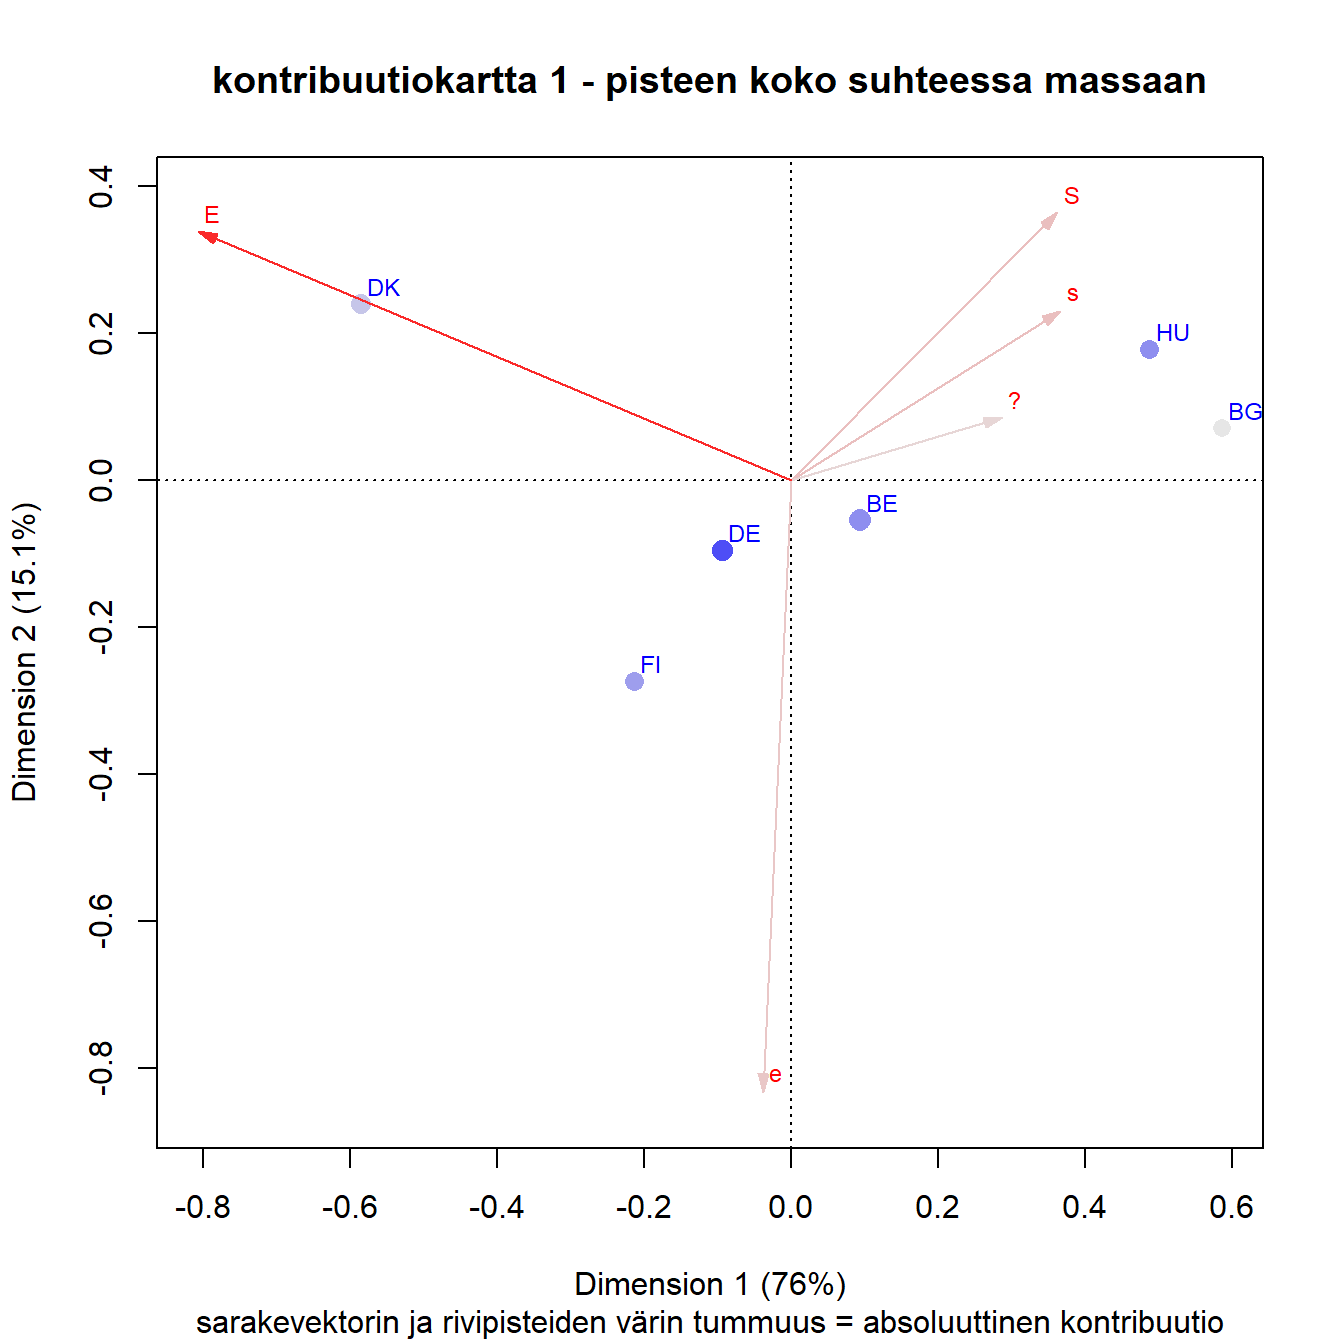
\includegraphics[width=0.9\linewidth]{JH_capaper_files/figure-latex/G1-3asymmContrib1-1} 

}

\caption{Q1b: lapsi kärsii jos äiti on töissä}\label{fig:G1-3asymmContrib1}
\end{figure}

Sarakkeista ratkaisuun vaikuttaa selvästi eniten E, ja juuri ensimmäiseen
dimensioon. Toista dimennsiota määrittää vahviten e, mutta myös kaikki muut
sarakkeet x-akselin yläpuolella. Samaa mieltä olevien (S ja s) vaikutus näyttäisi
jakautuvan selvimmin molemmille dimensioille.

Vaikka massojen suhteellisia eroja ei kovin helposti pistekoosta erota, se näkyy
epäsuorasti Saksan melko vahvimpana kontribuutiona. Bulgarian vähäisin kontribuutio
näyttäisi olevan ensimmäiselle dimensiolle.

\textbf{Suhteelliset kontribuutiot}

\begin{figure}

{\centering 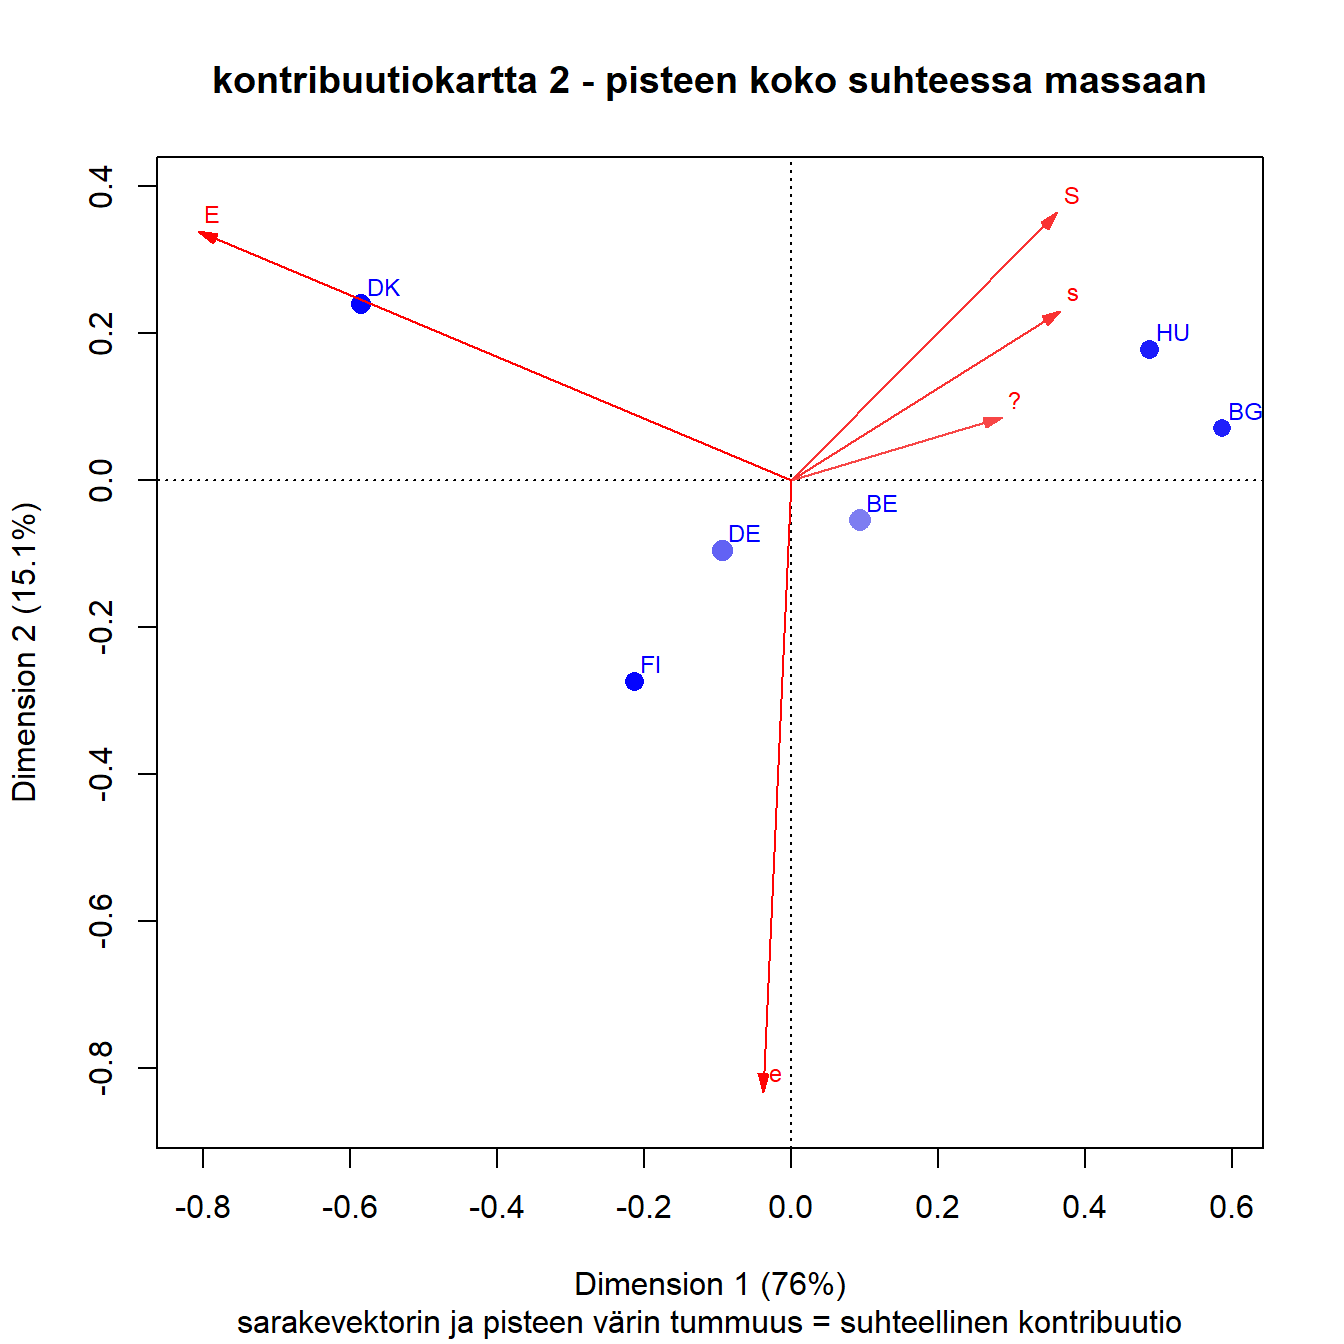
\includegraphics[width=0.9\linewidth]{JH_capaper_files/figure-latex/G1-3asymmContrib2-1} 

}

\caption{Q1b: lapsi kärsii jos äiti on töissä}\label{fig:G1-3asymmContrib2}
\end{figure}

Kaikki edellä esitetyt pääättelyt perustuvat tietysti kaksiulotteideen projektioon.
Jos pisteet on esitetty hyvin eli niiden inertiasta (poikkeamasta keskiarvosta)
suuri osa on kuvattu kartalle, rivipiste on sitä lähempänä ideaalipistettä mitä
suurempi ideaalipisteen osuus on sen profiilissa.

Sarakkeiden laatu näyttäisi olevan hyvä, mutta rivipisteistä Saksa ja erityisesti
Belgia erottuvat hieman heikommin esitettyinä.

\hypertarget{massat}{%
\section{Massat}\label{massat}}

\textbf{edit} Onko vakioitujen massojen kartta liian aikaisin? Tämä ei ole pääasia, vaan selvennys.
Miksi tässä? Perusteltava, miksi en vakioi massoja maille, sukupuolille jne. (a)
perusteltua kun tarkempi tutkimusongelma, esim. erottelut maiden ja sukupuolten
välillä. Varianssianalyysin tapaan varianssin hajoittaminen ryhmisen sisäiseen ja
ryhmien väliseen. Kts. teorialiitteestä esim. ABBA. (b) CA ``perusmuodossa'', massa
on yksi kolmesta tärkeimmästä käsitteestä. (c) on aika työlästä!

\textbf{edit} Galkussa verrattu molempien painotusten khii2-etäisyyksiä, jos tarpeen
niin teoria-liitteeseen.

Massat ovat korrespondenssianalyysin keskeinen käsite, ja niiden kaksoisrooli on
menetelmän ytimessä. Massat ovat normalisoiva muunnos khii2-etäisyysmitalle ja
profiilien painoja. Tässä jälkimmäisessä roolissa massat liittyvät tutkimusongelmaan,
mitä halutaan vertailla? Kun vertaillaan eri maita, ei ole kovin perusteltua käyttää
massoina eri maiden otoskokoja. Jos taas halutaan vertailla vaikkapa miesten ja
naisten vastauksia on luonnollista normalisoida miesten ja naisten massat yhtä
suuriksi. Rivi- ja sarakemassat ovat verrannollisia taulukon rivi- ja sarakesummiin,
frekvenssitaulukon reunajakaumiin. Ne voidaan tutkimusongelmaan sopivalla tavalla
skaalata uudelleen. CAiP(s. 23) esimerkissä viiden koulutustaso-ryhmän massat skaalataan
verrannollisiksi niiden väestötason osuuksiin, ei otoksen osuuksiin. Tällainen datan
esikäsittely on normaali osa korrespondenssianalyysin soveltamista.

Jos massat halutaan vakioida yhtä suuriksi osajoukoissa, ratkaisu on yksinkertainen.
Korrespondenssianalyysin taulukoksi otetaan riviprofiilitaulukko, jossa rivien summat
ovat yksi.

Kuvassa \ref{fig:simpleCA3map1} on tehty näin, ja kartta eroaa hämmästyttävän
vähän maiden otoskokoja massoina käyttävästä kartasta.

\begin{figure}

{\centering 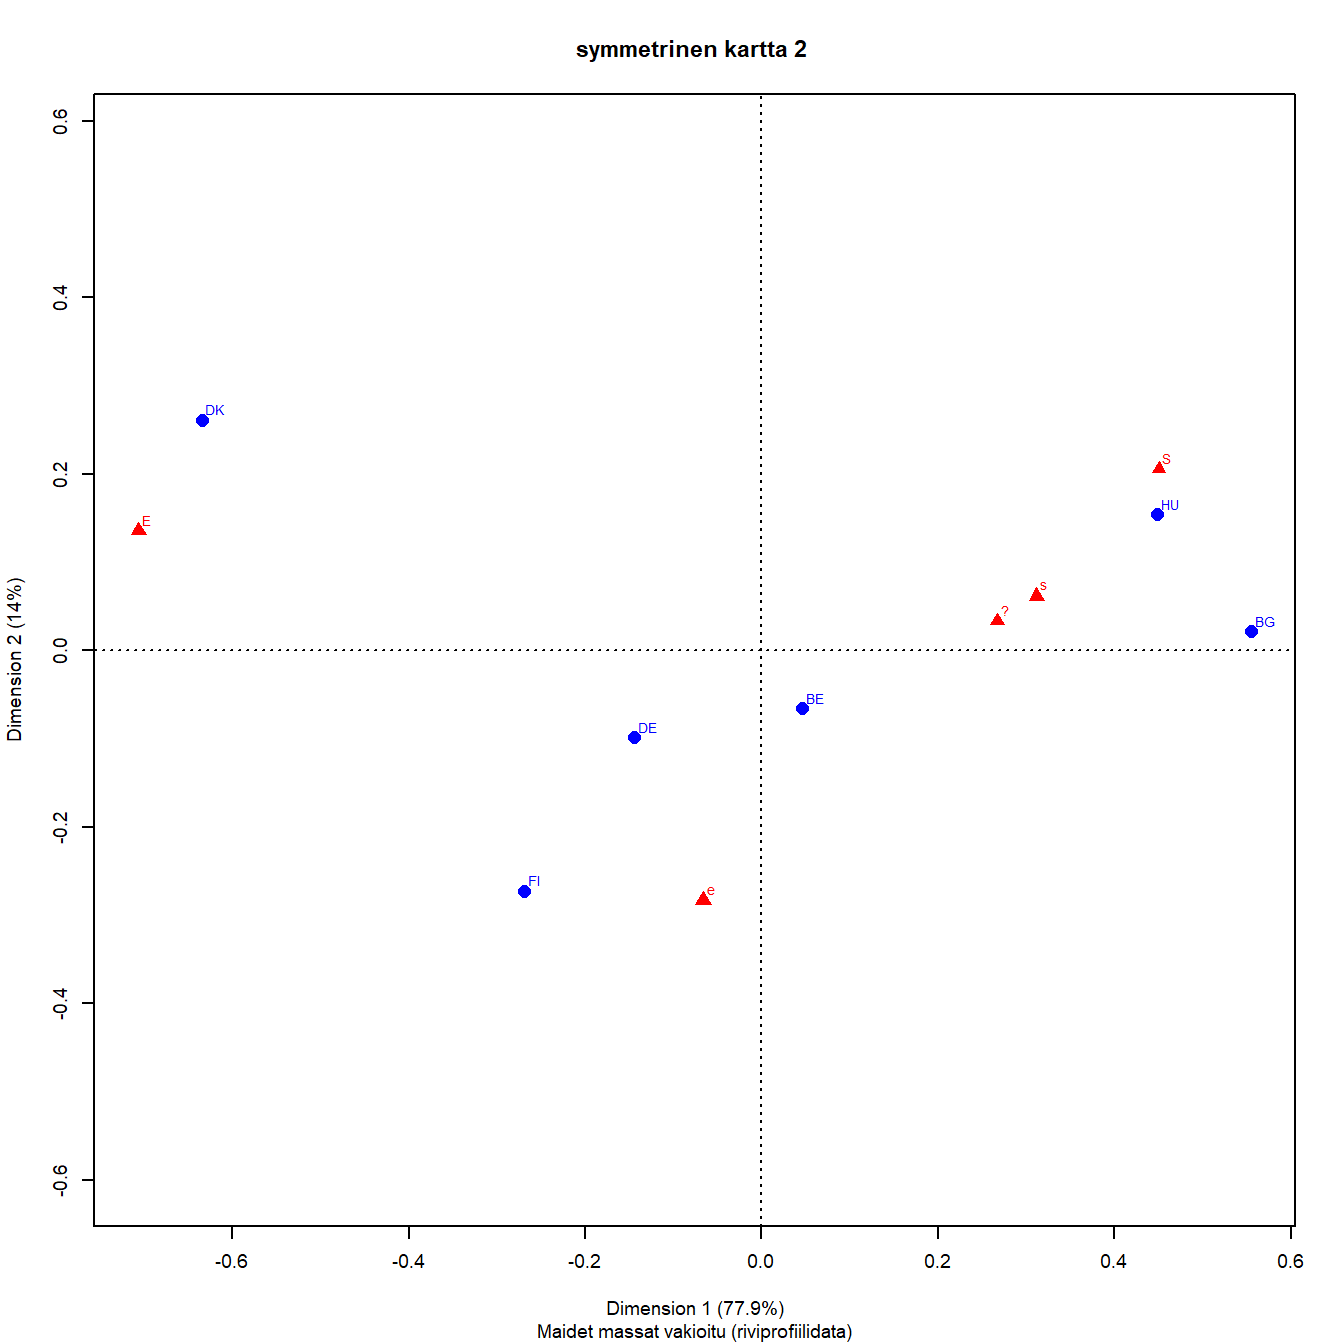
\includegraphics[width=0.9\linewidth]{JH_capaper_files/figure-latex/simpleCA3map1-1} 

}

\caption{Q1b: lapsi kärsii jos äiti on töissä}\label{fig:simpleCA3map1}
\end{figure}

Pienimpien otosten maat (Bulgaria, Unkari) liikahtavat hieman origoa kohti,
Bulgaria hieman enemmän kohti maltillista puolta x-akselia.

Kontribuutiokarttakaan ei eroa edellä esitetystä kartasta.
\textbf{edit} Tämä kuva on ehkä tarpeeton?

\begin{figure}

{\centering 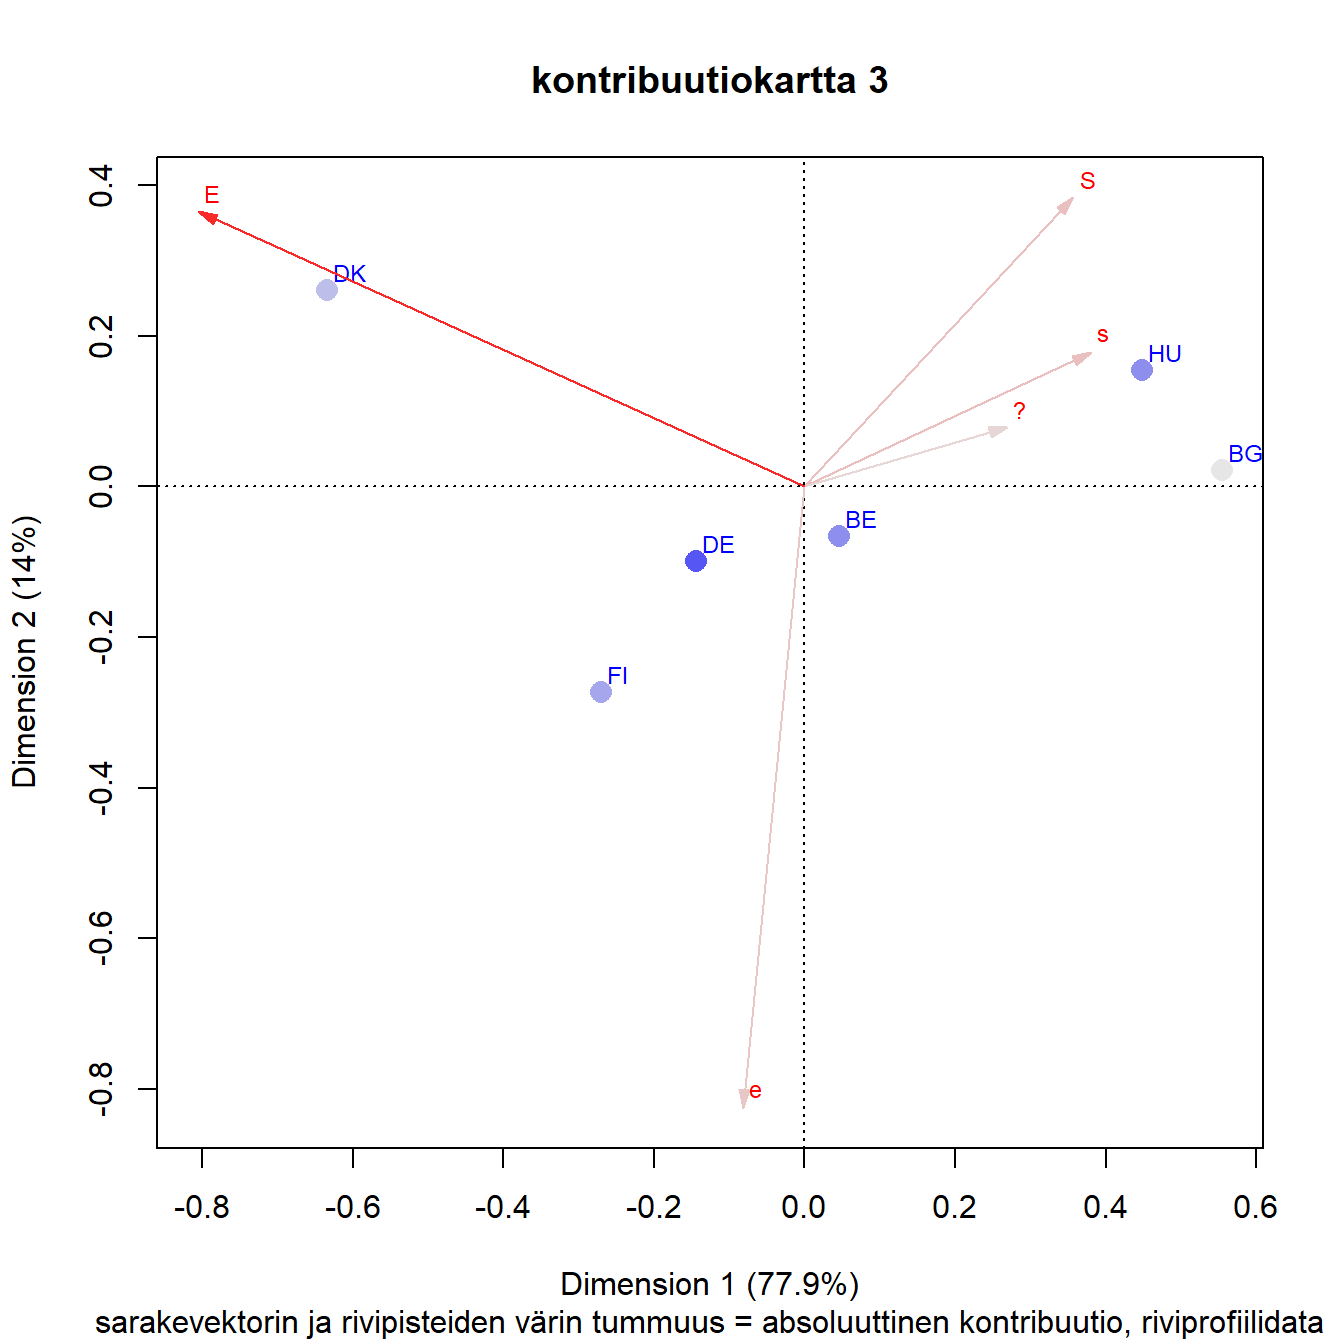
\includegraphics[width=0.9\linewidth]{JH_capaper_files/figure-latex/simpleCA3map2-1} 

}

\caption{Q1b: lapsi kärsii jos äiti on töissä}\label{fig:simpleCA3map2}
\end{figure}

En ole vakioinut vertailtavien ryhmien (tässä maat) suhteellisia osuuksia. Syy on
yksinkertainen: esittelen menetelmää sen perusmuodossa ilman kovin täsmällisiä
tutkimusongelmia. Oikeiden tutkimuskymysten vastausia pitää tietysti etsiä järkevillä
massojen skaalauksella. Korrespondenssianalyysi on inertian eli kokonaishajonnan
dekomponointia, jakamista osiin.

\hypertarget{karttojen-erot}{%
\section{Karttojen erot}\label{karttojen-erot}}

Yksinkertaisen korrespondenssianalyysin peruskuva on symmetrinen kartta. Ehkä
yllättäen sen ``\ldots tulkinta on edelleen menetelmän kaikkein kiistanalaisin aspekti.''
\citep{RefWorks:doc:5a857a43e4b0ed2d44664d78} (s.295),\citep{RefWorks:doc:5c768b09e4b02df9431e950a}.
vrt. myös, Johdanto, SPSS - kritiikki.

Sarake- ja rivisteet esitetään siinä ikään kuin päällekkäin, samassa koordinaatistossa.
Niiden pääkoordinaatit ovat kuitenkin eri pistejoukoista tai avaruuksista. Asymmetrisessä
kartassa pisteet ovat samassa avaruudessa, ja ero on Greenacren mukaan vain skaalaus.
Asymmetrisessä kartassa standardikoordinaateissa esitetyt ideaalipisteet skaalataan
pääakselien suunnassa vastaavilla pääakselien inertioiden neliöjuurilla. Siten pisteiden
suuntavektorit niin pääkoordinaateissa kuin standardikoordinaateissa ovat lähes samat
kun akselien inertioiden (principal inertias) neliöjuuret eivät ole liian erisuuruisia.

Jos pääinertioiden neliöjuuret ovat hyvin eri suuruisia, tulkintaongelmia voi tulla, mutta
niillä ei käytännössä ole merkitystä. Siksi hän pitää skaalausdebattia akateemisena
kiistana, käytännön sovelluksissa sillä ei ole merkitystä. Kiista on ollut aika
sitkeä (esimerkiksi 1989 Greenacren kommentoi skaalausta perusteellisesti \citep{RefWorks:doc:5c754c6de4b0947789165cde}), mutta lienee laantunut.

Symmetinen kartta hyvä vaihtoehto, sillä asymmetrisessä skaalaus vie
ideaalipisteet usein kauas pääkoordinaateissa esitetyt pisteet pakkautuvat kuvan
keskelle. Toisaalta jos dataa tulkitaan ''asymmetrisesti'' kontribuutiokartta on
hyvä vaihtoehto. Silloin rivipisteiden etäisyydet esitetään optimaalisesti,
sarakkeiden suuntavektoreille projisoiduilla pistellä on kaksoiskuva-tulkinta
(biplot) ja niiden pituudetkin kertovat jotain.

Greenacren mukaan kartoilla voi tavoitella kolmea eri asiaa, joista vain kaksi
voi totetua yhtä aikaa. Kuvassa voi esittää rivipisteiden etäisyydet,
sarakepisteiden etäisyydet tai rivi- ja sarakepisteiden etäisyydet. Jäkimmäinen on
kaksoiskuvien (biplot) ns. skalaaritulo-ominaisuus. Rivi- ja sarakepisteen
skalaaritulo ``palauttaa'' alkuperäisen datan, tässä tapauksessa taulukon solun.

Näistä vain kaksi voidaan optimaalisesti esittää yhtä aikaa.

\emph{Symmetrisessä kartassa} khii2-etäisyydet rivipisteiden välillä ja sarakepisteiden
välillä esitetään optimaalisesti. Rivi- ja sarakepisteiden välisiä etäisyyksiä ei
esitetä optimaalisesti, mutta ne voidaan tulkita kohtalaisen hyvin jos pääakselien
inertioiden neliöjuuret eivät ole liian erisuuruisia.

\emph{Asymmetrisessä kartassa} pääkoordinaateissa esitetyn pistejoukon etäisyydet
kuvataan optimaalisesti, standardikoordinaateissa esitetyt pisteet ovat ``ääriprofiileja'',
verteksin kulmapisteitä. Rivi- ja sarakepisteiden etäisyydet esitetään optimaalisesti,
mutta sarakepisteiden etäisyyksillä ei ole suoraa tulkintaa,

\emph{Kontribuutiokartta} on muunnelma asymmetrisestä kartasta. ``Ääriprofiilit'' vedetään
kohti origoa kertomalla ne massojen neliöjuurilla. Näin kuva selkenee, ja ``kutistetun''
pisteen etäisyys origosta (``vektori'') kertoo sen kontribuution pääakseleille. Näiden pisteiden
välisillä etäisyyksillä ei ole suoraa tulkintaa.

\hypertarget{tuxe4ydentuxe4vuxe4t-pisteet}{%
\chapter{Täydentävät pisteet}\label{tuxe4ydentuxe4vuxe4t-pisteet}}

Kartat ovat analyysin väline, ja usein on hyödyllistä esittää kuvassa
lisäinformaatiota tulkinnan avuksi. Täydentävät pisteet (supplementary points,
CAiP s. 89-) ovat rivejä tai sarakkeita jotka lisätään karttaan. Mikä tahansa
rivi tai sarake voidaan voidaan lisätä kuvaan, jos se on järkevästi vertailukelpoinen
kartan määtittäneiden profiilien kanssa.

Tällainen piste on kartan laskennassa \emph{passiivinen}, sillä on sijainti kartalla
mutta ei massaa eikä vaikutusta inertiaan. Passiivisilla pisteillä ei ole vaikutusta
(kontribuutiota) kartan pääakseleihin.

Täydentävillä pisteillä on kolme yleistä käyttötarkoitusta. Kartalle voidaan lisätä
profiili, joka on jollain lailla sisällöllisesti erilainen kuin muut. Esimerkkiaineistossa
kartalle voisi lisätä joitain Euroopan ulkopuolisia maita. Vaikka nämä riviprofiilit
eivät vaikuta kartan akseleiden määräytymiseen, ne voidaan esittää kuuden maan
määrittämässä ``avaruudessa''. Projektion laatu (suhteelliset kontribuutiot) voidaan myös
esittää.

Toinen käyttötapaus on pienen massan profiili. Tällaisella pisteellä voi olla iso
vaikutus ratkaisuun, mutta passiivisena pisteenä se sijoitetaan muiden pisteiden
määrittämälle kartalle. Jo sisällöllisistä syistä pienen massan pisteiden esitystä
kannattaa harkita, ne sijaitsevat kaukana origosta ja huonontavat kuvan laatua.
Esimerkkiaineistossa puuttuvat vastaukset voisi ottaa mukaan täydentävänä pisteenä.

Kolmas mahdollisuus on jakaa pistejoukkoja osajoukkoihin ja esittää niiden
summaprofiili täydentävänä pisteenä. Summaprofiili on osiensa painotettu
(barysentrinen) keskiarvo. Kun se esiteteään passiivisena pisteenä, havaintoja ei
oteta ratkaisuun kahta kertaa. Profiilien yhdistämiseen liittyy
korrespondenssianalyysin tärkein periaate, jakaumaekvivalenssi (\emph{distributional
equivalence}). Profiileiltaan samanlaiset rivit voidaan yhdistää, analyysin tulokset
eivät muutu. Khii2-etäisyysmitta taas on ainoa etäisyysmitta joka toutettaa tämän
periaatteen. En esittele tätä ydinkäsitettä tämän enempää (kts. esim. CAiP tai
perusteellinen matemaattinen esitys \citep{RefWorks:doc:5a857a43e4b0ed2d44664d75}).

Täydentävien profiilien lisääminen vaatii jo yksinkertaisia matriisioperaatioita.
Korrespondenssianalyysi on käytännössä matriisien muokkausta tutkimusongelman
tarpeisiin.

\hypertarget{saksan-ja-belgian-alueet}{%
\section{Saksan ja Belgian alueet}\label{saksan-ja-belgian-alueet}}

Saksan ja Belgian aineistossa on mukana aluejako: entiset itä- ja länsi-Saksa
(dE,dW), Flanders (bF), Wallonia (bW) ja Bryssel (bB).

\begin{table}

\caption{\label{tab:BeDealueTable1}Q1b vastaukset, Saksan ja Belgian alueet}
\centering
\begin{tabular}[t]{lllllll}
\toprule
  & S & s & ? & e & E & Total\\
\midrule
bF & 5.04 & 23.81 & 25.89 & 30.83 & 14.43 & 100.00\\
bW & 10.82 & 21.02 & 18.57 & 24.08 & 25.51 & 100.00\\
bB & 17.03 & 20.94 & 16.63 & 23.87 & 21.53 & 100.00\\
BG & 12.81 & 42.89 & 22.26 & 20.63 & 1.41 & 100.00\\
dW & 11.40 & 26.82 & 11.83 & 32.13 & 17.82 & 100.00\\
\addlinespace
dE & 5.85 & 11.33 & 10.97 & 29.80 & 42.05 & 100.00\\
DK & 5.04 & 17.15 & 10.95 & 16.71 & 50.14 & 100.00\\
FI & 4.23 & 16.94 & 13.42 & 38.11 & 27.30 & 100.00\\
HU & 21.97 & 28.89 & 22.57 & 19.06 & 7.52 & 100.00\\
All & 9.95 & 23.76 & 16.79 & 26.10 & 23.41 & 100.00\\
\bottomrule
\end{tabular}
\end{table}

Aineistoon lisätään passiviisina riveinä Saksan ja Belgian maaprofiilit (DE, BE).
Maiden massoja ei skaalta yhtä suuriksi, otoskoot vaikuttavat ratkaisuun.

\begin{figure}

{\centering 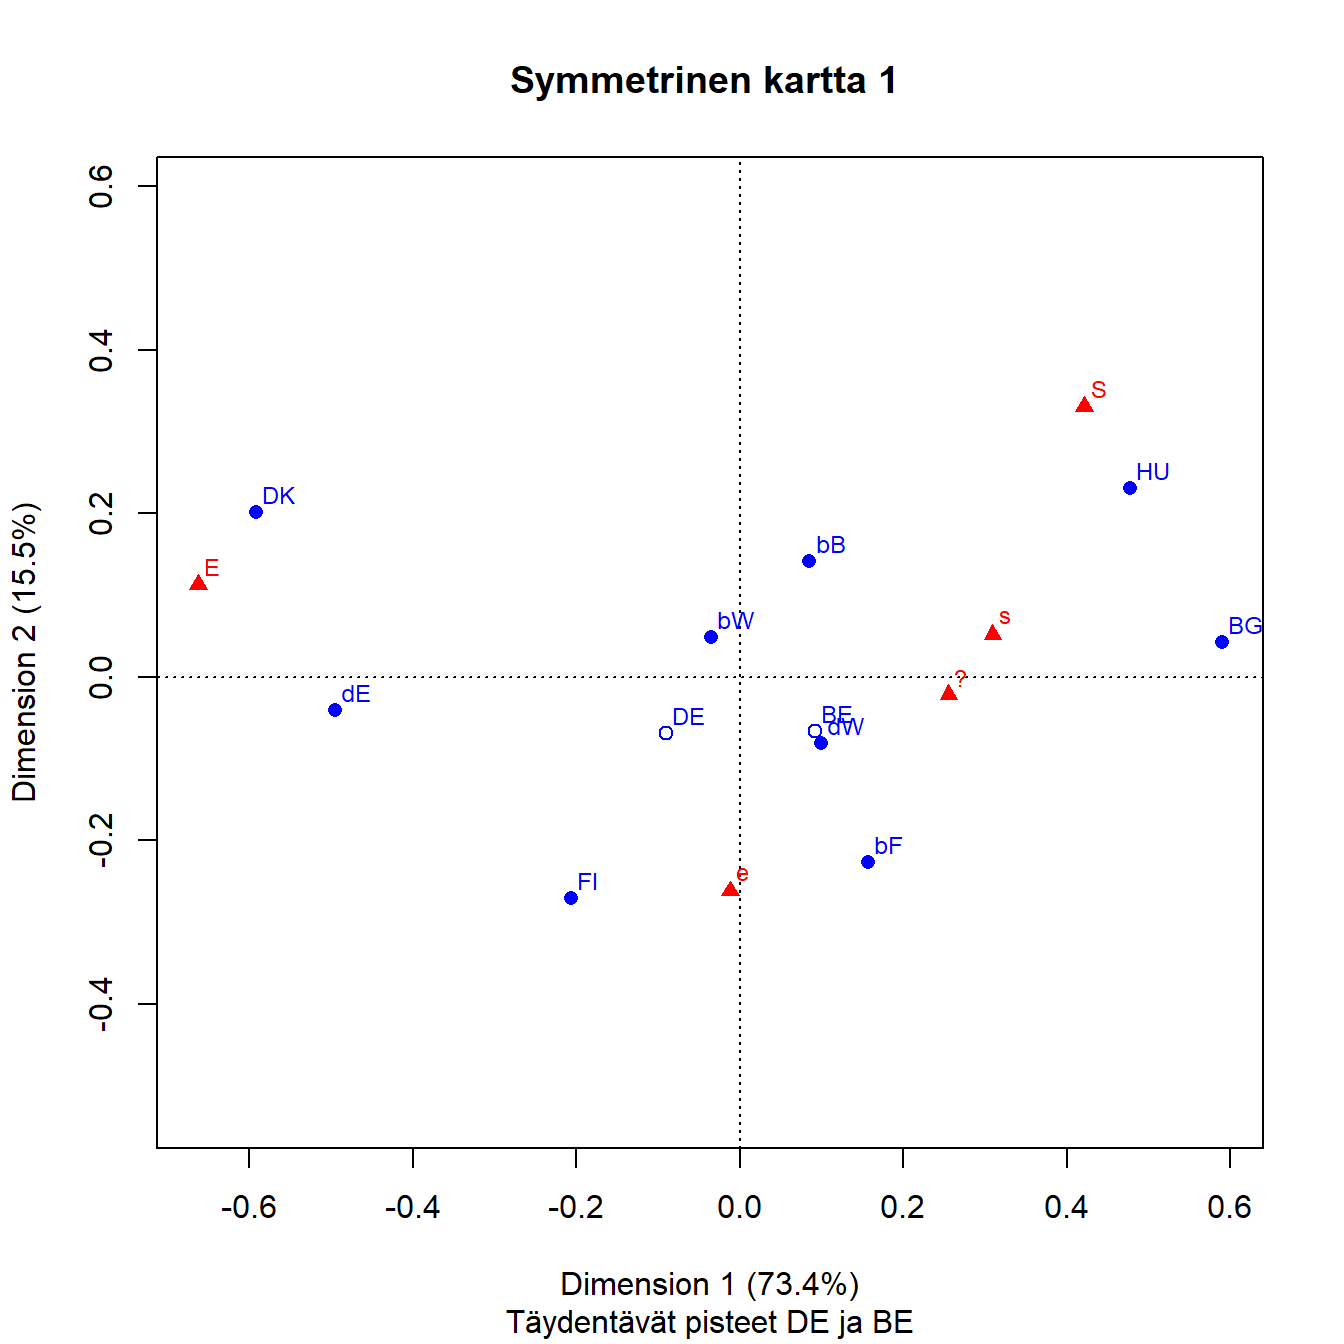
\includegraphics[width=0.9\linewidth]{JH_capaper_files/figure-latex/suppointCA2map1-1} 

}

\caption{Q1b: Saksan ja  Belgian aluejako }\label{fig:suppointCA2map1}
\end{figure}

Saksan ja Belgian täydentävät pisteet ovat osiensa barysentrisiä keskiarvoja,
etäisyys on sitä pienempi mitä suurempi on osuus. Saksan piste sijaitsee siksi
lähempänä länsi-Saksan pistettä. Karttaa kannattaa verrata kuvaan jossa aluejakoa
ei ole \ref(fig:simpleCA1map1), mutta Saksan ja Belgian osien sijoittuminen on kiinnostava.
Itäinen Saksa on selvästi liberaalilla puolella, ensimmäisellä dimensiolla lähinnä Tanskaa.
Läntinen Saksa on ensimmäisellä dimensiolla konservatiivisella puolella Belgian maapisteen
tasolla. Belgian alueista Wallonia (bW) on liberaalilla puolella mutta kaikkein eniten oikealla.
Bryssel ja Flander ovat konservatiivisella puolella, toinen länsi-Saksaa liberaalimpi ja toinen konservatiivisempi. Belgian osat hajoavat toiseen suuntaan kuin Saksan,
liberaalein Flanders on myös kaikkein maltillisin ja Bryssel vastaavasti
tiukempien mielipiteiden puolella. Sarakepisteiden suhteelliset sijainnit
toisiinsa nähden eivät oleellisesti muutu.

Bryssel ja Wallonia näyttävä olevan hyvin lievästi U-muotoisen maapisteiden
parven sisällä. Tämä kaariefekti tai \emph{Guttman-efekti} on kartoissa yleinen.
Se on tavallaan seuraus ratkaisun geometriasta. Rivipisteiden pilvi on
sarakkeiden ideaalipisteiden virittämän verteksin sisällä, ja ainoa reitti
verteksin kulmasta toiseen kulkee tasolla kaarveasti (VIITE: MG, CAiP).
Voi myös sanoa, että kaariefektin taustalla on järjestysasteikon muuttujan
korrelaatio (viite: LeRoux). Kaaren sisäpisteet ovat usein polarisoituneita
ensimmäisen dimension ``ääripää-vastausten'' välillä. Tässä vaikutus on heikko,
taulukossa \ref{tab:BeDealueTable1} ei mitää selvää polariaatiota näy.

\begin{figure}

{\centering 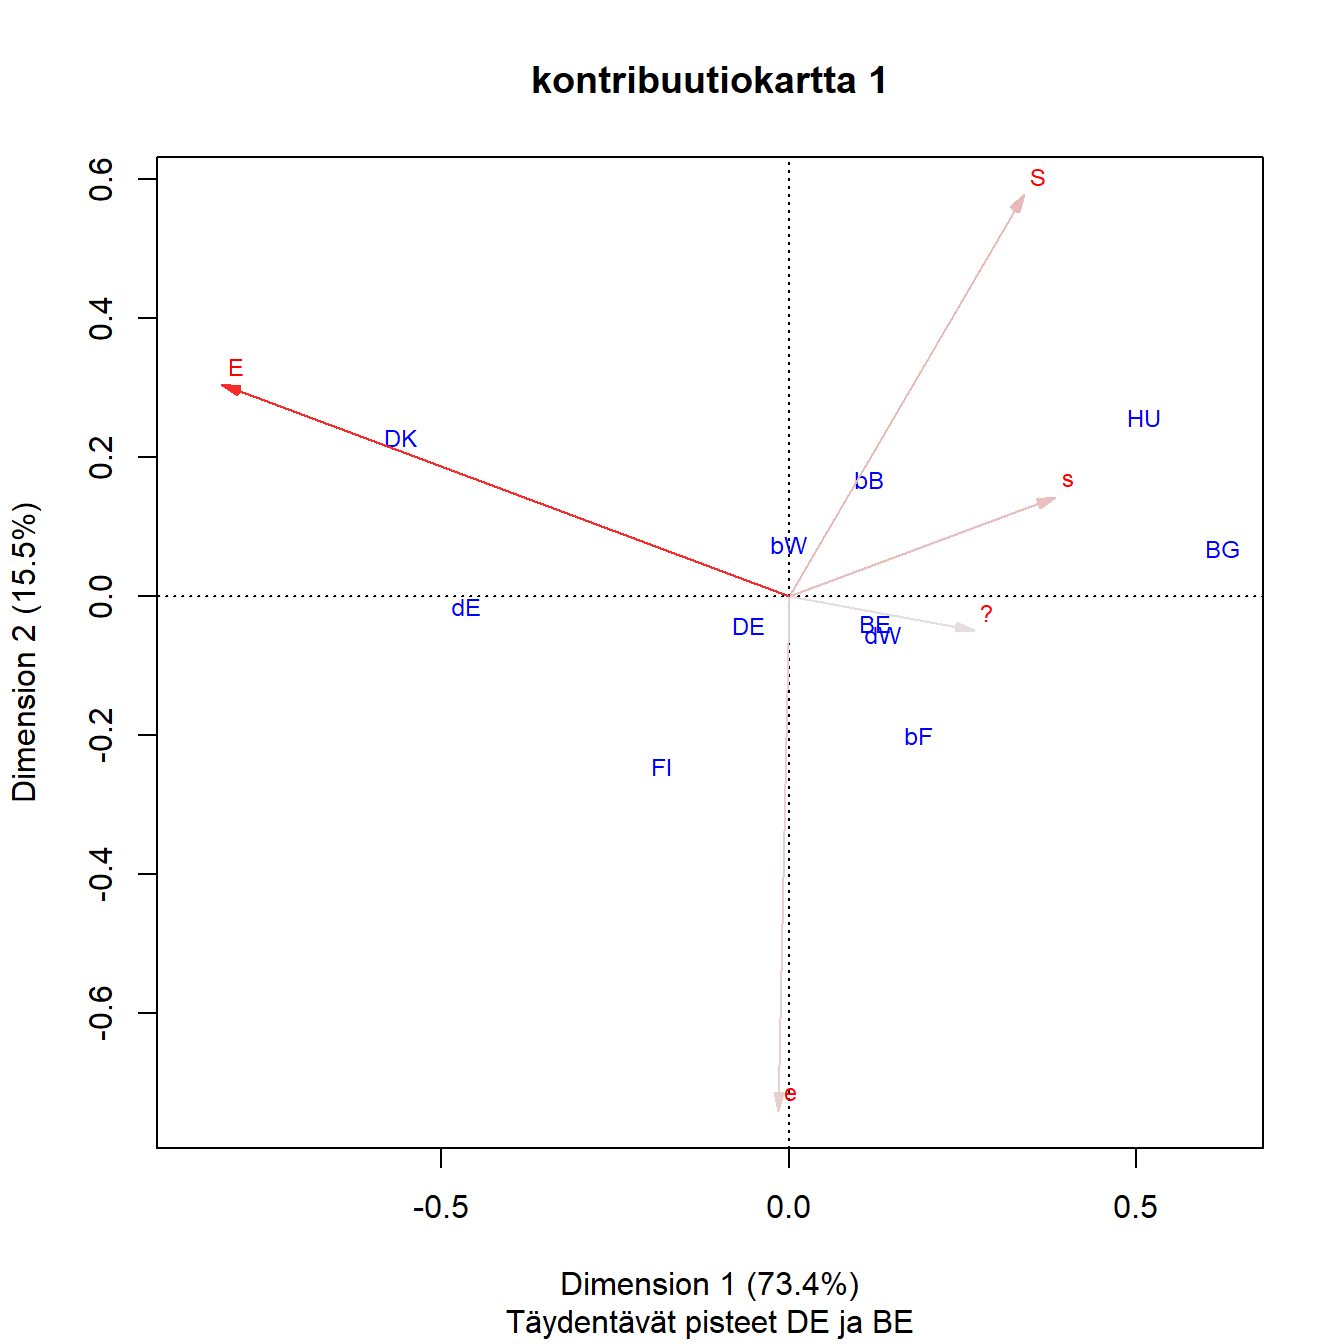
\includegraphics[width=0.9\linewidth]{JH_capaper_files/figure-latex/suppointCA2map2-1} 

}

\caption{Q1b: Saksan ja  Belgian aluejako }\label{fig:suppointCA2map2}
\end{figure}

Kontribuutiokartasta täydentävät pisteet on jätetty pois, ne eivät vaikuta ratkaisuun.
Pisteiden koko auttaa hahmottamaan niiden massojen eroja, sarakkeiden massoja ei
juuri tässä kuvassa erota. Sarakkeiden kontribuutiot ovat samantapaiset kuin
alkuperäisessä kartassa \ref{fig:G1-3asymmContrib1}. Rivipisteiden kontribuutioista
osa on selvästi pienempiä, erityisesti länsi-Saksa kaksi Belgian aluetta (bB, bF).
Unkarin ja Bulgarian kontribuutiot muuttuvat eri suuntiin, Unkarin pienenee ja
Bulgarian kasvaa.

\hypertarget{korrespondenssianalyysin-numeeriset-tulokset}{%
\section{Korrespondenssianalyysin numeeriset tulokset}\label{korrespondenssianalyysin-numeeriset-tulokset}}

Korrespondenssianalyysin numeeriset tulokset ovat tärkeitä tulkinnan varmistamiselle
ja antavat tarkemman kuvan ratkaisusta. Nämä tulokset ovat erilaisia kokonaisinertian
dekomponointeja. Kokonaisinertia (total inertia) profiilien ja keskiarvoprofiilin
khii2-etäisyyksien massoilla painotettu summa (\eqref{eq:inert2}. Se kuvaa
profiilipisteiden hajontaa ideaalipisteiden verteksin sisällä. Maksimi-inertia
saavutetaan kun profiilit ovat verteksien kärkipisteissä, jokaisessa profiilissa on vain
yksi luokittelumuuttujan arvo. Inertia on sama kuin ratkaisun dimensio, tässä esimerkissä
4 (sarakkeiden lukumäärä - 1).\footnote{Luku perustuu CAiP:n lukuun 11 ja liitteeseen B}.

R-paketti ``ca'' (versio 0.71.1) listaa numeeriset tulokset suppeasti (print) ja laajemmin
(summary), laajempi tulostus on alla.\footnote{Paketin pdf-dokumentissa s.20 kerrotaan, että print
  tulostaa pääkoordinaatit (principal coordinates) mutta se tulostaakin standardikoordinaatit.}

\textbf{k} Lyhyt selostus - nämä aika selkeitä

Ensimmäisenä on listattu kokonaisinertia pääakseleittain. Tässä suhteelliset luvut
on esitetty prosentteina. Muut luvut on luettavuuden vuoksi skaalattu, joko kerrottu
tuhannella tai esitetty ``permills'' (summa on 1000).

\begin{Shaded}
\begin{Highlighting}[]
\KeywordTok{summary}\NormalTok{(suppointCA2)}
\end{Highlighting}
\end{Shaded}

\begin{verbatim}
## 
## Principal inertias (eigenvalues):
## 
##  dim    value      %   cum%   scree plot               
##  1      0.154101  73.4  73.4  ******************       
##  2      0.032489  15.5  88.9  ****                     
##  3      0.014294   6.8  95.7  **                       
##  4      0.008944   4.3 100.0  *                        
##         -------- -----                                 
##  Total: 0.209828 100.0                                 
## 
## 
## Rows:
##       name   mass  qlt  inr    k=1 cor  ctr    k=2 cor  ctr  
## 1  |    bF |  124  650   69 |  157 212   20 | -226 438  195 |
## 2  |    bW |   60  388    3 |  -36 137    0 |   48 252    4 |
## 3  |    bB |   63  481   17 |   85 127    3 |  142 354   39 |
## 4  |    BG |  113  878  215 |  590 874  255 |   43   5    6 |
## 5  |    dW |  143  345   33 |  100 208    9 |  -81 138   29 |
## 6  |    dE |   67  966   82 | -495 960  107 |  -41   7    3 |
## 7  |    DK |  170  971  327 | -591 869  387 |  202 102  214 |
## 8  |    FI |  136  957   79 | -206 352   38 | -271 605  307 |
## 9  |    HU |  122  927  177 |  477 751  181 |  231 176  201 |
## 10 | (*)BE | <NA>  512 <NA> |   92 338 <NA> |  -66 173 <NA> |
## 11 | (*)DE | <NA>  418 <NA> |  -90 265 <NA> |  -68 153 <NA> |
## 
## Columns:
##     name   mass  qlt  inr    k=1 cor ctr    k=2 cor ctr  
## 1 |    S |   99  816  167 |  421 505 115 |  331 311 335 |
## 2 |    s |  238  781  143 |  309 759 147 |   52  22  20 |
## 3 |      |  168  594   88 |  255 589  71 |  -22   4   2 |
## 4 |    e |  261  871   98 |  -12   2   0 | -262 870 550 |
## 5 |    E |  234  999  505 | -663 971 667 |  113  28  93 |
\end{verbatim}

Rivi- ja sarakeprofiileista esitetään samat tiedot. Ensimmäisessä kolmen
sarakkeen joukossa kerrotaan pisteen massa, laatu (qlt) ja inertiakontribuutio.

Inertiakontribuutio on suhteellinen osuus kokonaisinertiasta. Aktiivisia rivejä on 9,
joten tasaisesti jaettu inetia olisi noin 110. Tanska, Bulgaria ja Unkari ``selittävät''
suurimman osan inertiasta. Belgian ja Saksan alueiden kontribuutiot ovat pieniä.
Nämä inertiaosuudet liittyvät kokonaisinertiaan alkuperäisessä neljässä ulottuvuudessa.

Laatu kertoo miten hyvin piste on esitetty kartalla, miten suuri osa sen
inertiasta on esitetty kartalla. Kaksiulotteinen kartta kuten tässä on yleisin
valinta, laatu kerrotaan valitulle dimensioiden määrälle. Laatu ei riipu massasta,
vaan pisteen ja kartan akseleiden välisistä kulmista (kts. teorialiite). Saksan
osien ero laadussa on iso,itä-Saksalla erittäin hyvä ja länsi-Saksalla huono.
Belgian alueista Wallonia on kehtoiten esitetty, ja vain Flandersin laatu on
kohtuullisen hyvä. Kovin hyvä ei ole täydentävien maapisteidenkään laatu.

Kaksi seuraavaa lohkoa kertovat tulokset valituille dimenisoille eli ratkaisulle.
Molempien dimensioiden (``k=1'', ``k=2'' ) pääkoordinaattattien (x 1000) lisäksi
raportoidaan dimension \emph{suhteellinen kontribuutio} pisteen inertiaan (``cor'').
Nämä tunnusluvut summautuvat laaduksi (qlt), ja ne voidaan tulkita korrelaation
neliöiksi (kts. teorialiite).Erityisesti Belgian alueiden projektion laatu on
huonompi ensimmäisellä dimensiolla. Itä-Saksa ja Bulgaria taas ovat hyvin esittyjä
vain ensimmäisellä dimensiolla eivätkä juuri ollenkaan korreloi toisen dimension
kanssa.

Pisteen \emph{absoluuttinen kontribuutio} kertoo sen osuuden dimension inertiasta
(summa 1000). Jos katsotaan sarakkeita, nähdään E-sarake ``selittää'' ensimmäisen
dimension inertiasta lähes 70 prosenttia, ja dimensio saman verran
kokonaisinertiasta.

\textbf{k} Tulosteen käsitteiden esittely - tavoite kuvan laadun varmistus, akselien
tulkinnan tarkistus. Tarkemmin teorialiitteessä. Tästä pitäisi nähdä, miksi seuraavat
kartat ovat sellaisia kuin ovat.

\hypertarget{esimerkki-3d--kartasta---saksan-ja-belgian-dimensiot}{%
\section{Esimerkki 3d- kartasta - Saksan ja Belgian dimensiot}\label{esimerkki-3d--kartasta---saksan-ja-belgian-dimensiot}}

\textbf{k} Ei kovin hyviä kuvia, mutta periaate on tärkeä. Kartta on approksimaatio,
pitää päättää milloin se on tarpeeksi hyvä. Tai mille pisteille hyvä, mille huonompi.

\textbf{edit 26.10.2020} summary-funktio ei toimi, kun dimensioita CA-ratkaisussa kolme.
Numeeriset tulokset voisi laskea ``käsityönä''. Kehno kvalitetti 2d-ratkaisussa saa
kuvissa selityksen.

\begin{Shaded}
\begin{Highlighting}[]
\NormalTok{suppointCA3 <-}\StringTok{ }\KeywordTok{ca}\NormalTok{(}\OperatorTok{~}\NormalTok{maa3 }\OperatorTok{+}\StringTok{ }\NormalTok{Q1b,ISSP2012esim1.dat, }\DataTypeTok{nd =} \DecValTok{3}\NormalTok{)}

\CommentTok{# summary(suppointCA3)}
\CommentTok{# Error in rsc %*% diag(sv) : non-conformable arguments}
\CommentTok{# outo juttu, ei toimi! - TÄMÄ POISTETAAN}
\end{Highlighting}
\end{Shaded}

\textbf{Kolme karttaa}

\begin{figure}

{\centering 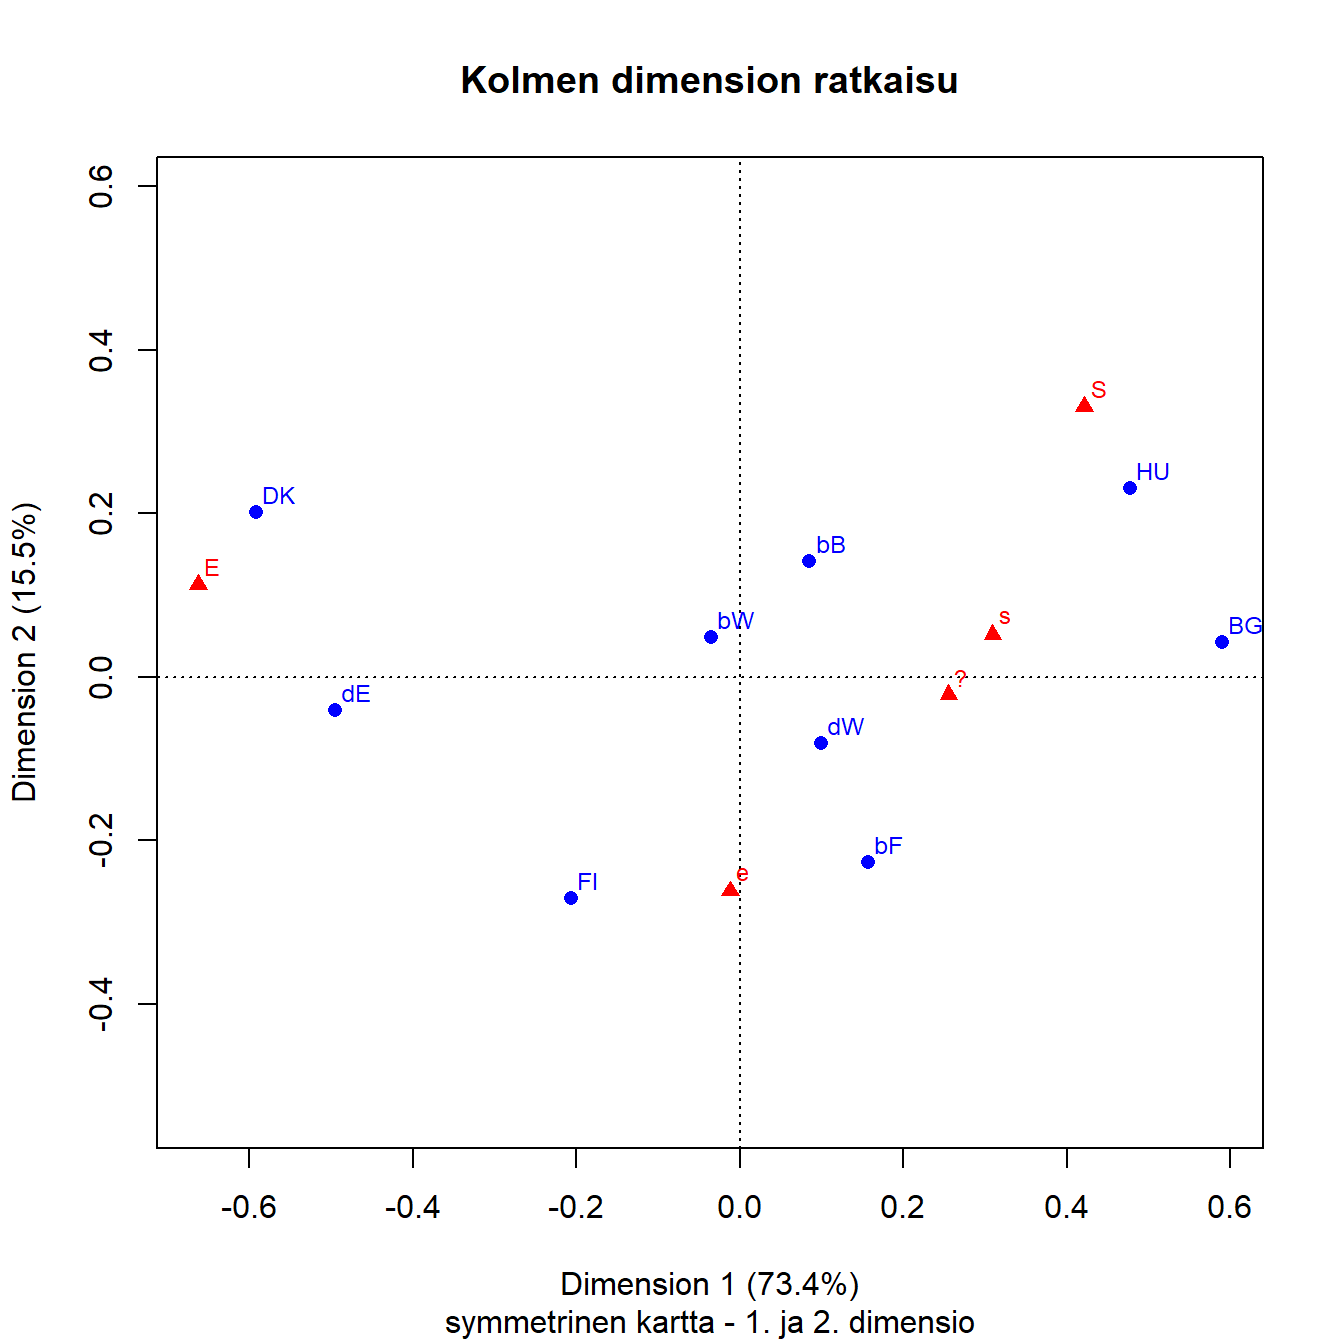
\includegraphics[width=0.9\linewidth]{JH_capaper_files/figure-latex/suppointCA3map1-1} 

}

\caption{Q1b: Saksan ja  Belgian aluejako }\label{fig:suppointCA3map1}
\end{figure}

\begin{figure}

{\centering 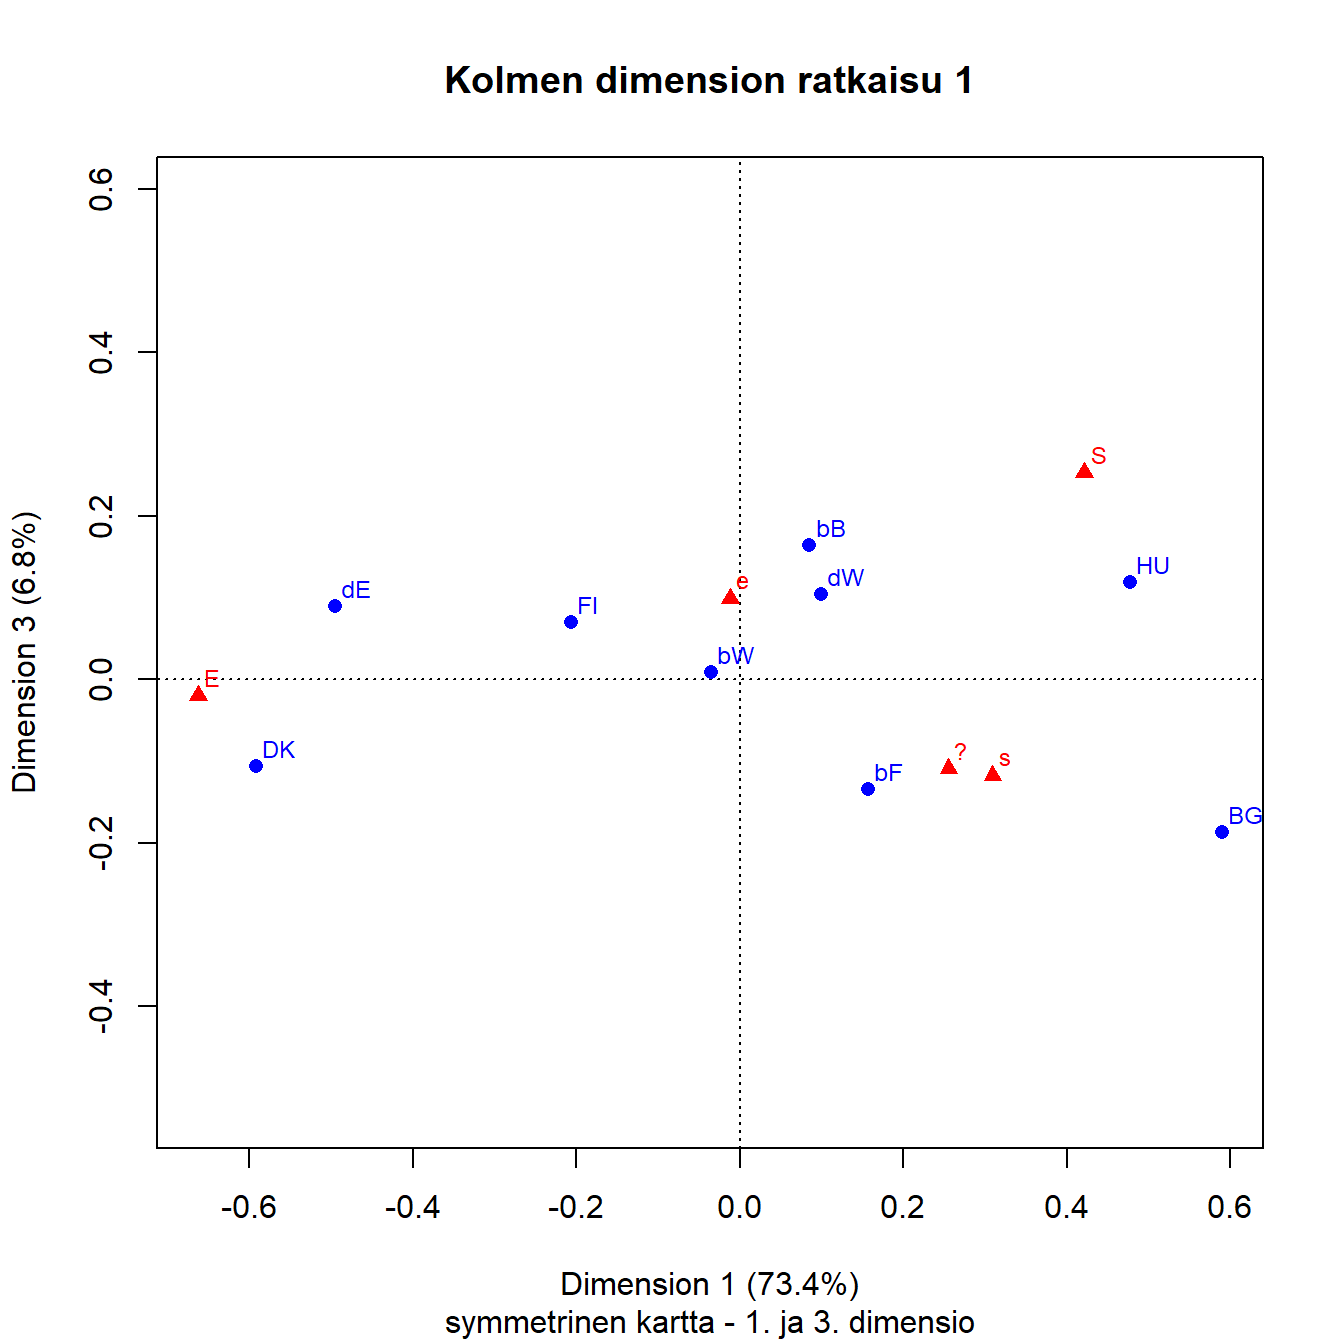
\includegraphics[width=0.9\linewidth]{JH_capaper_files/figure-latex/suppointCA3map2-1} 

}

\caption{Q1b: Saksan ja  Belgian aluejako }\label{fig:suppointCA3map2}
\end{figure}

\begin{figure}

{\centering 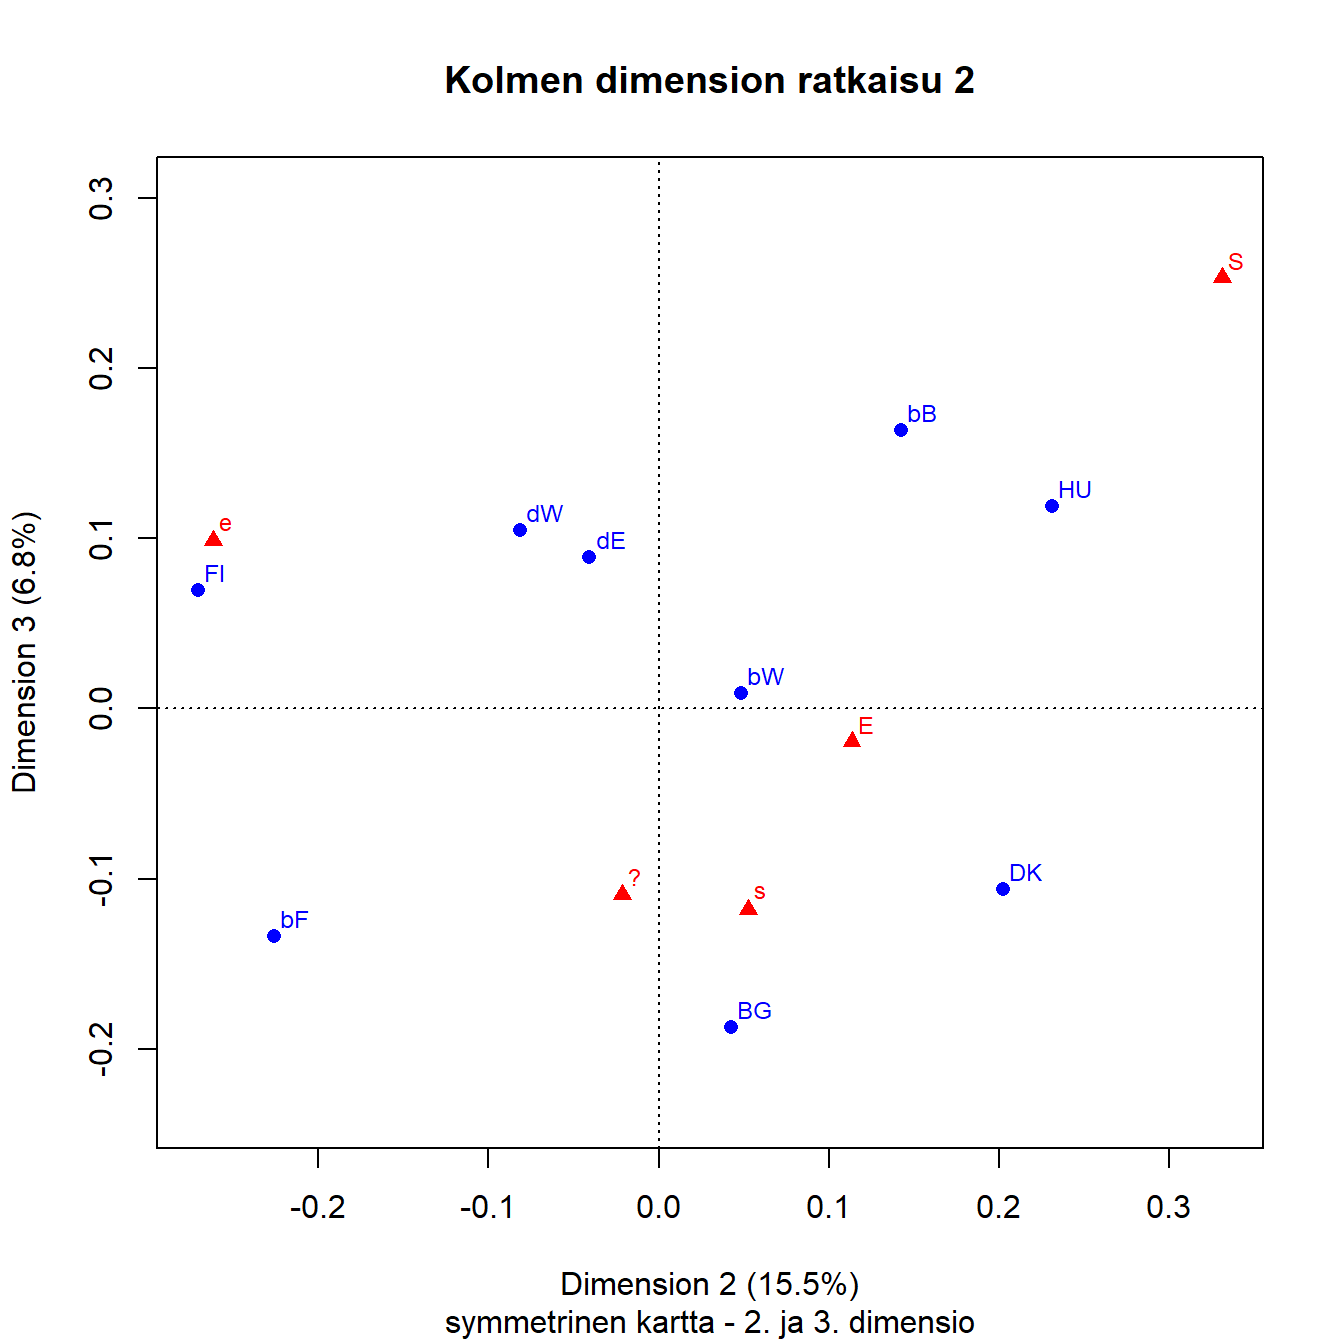
\includegraphics[width=0.9\linewidth]{JH_capaper_files/figure-latex/suppointCA3map3-1} 

}

\caption{Q1b: Saksan ja  Belgian aluejako }\label{fig:suppointCA3map3}
\end{figure}

\textbf{k} Tulkinta.

\textbf{k} kokeilu 3d-grafiikalla - toinen riittää

\begin{figure}

{\centering 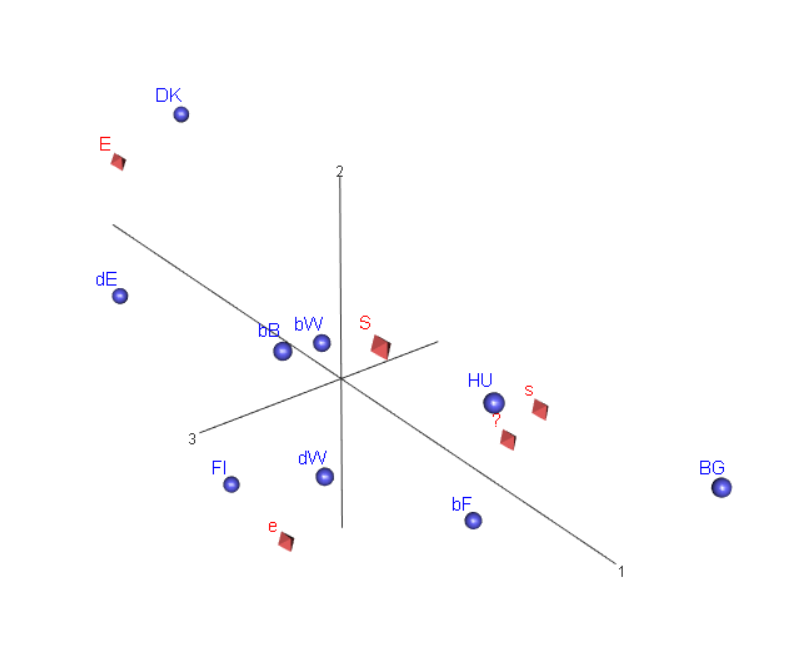
\includegraphics[width=0.9\linewidth]{img/3dSymMap_1} 

}

\caption{Saksan ja  Belgian aluejako - 3d-kuva1}\label{fig:3dklippi1}
\end{figure}

\begin{figure}

{\centering 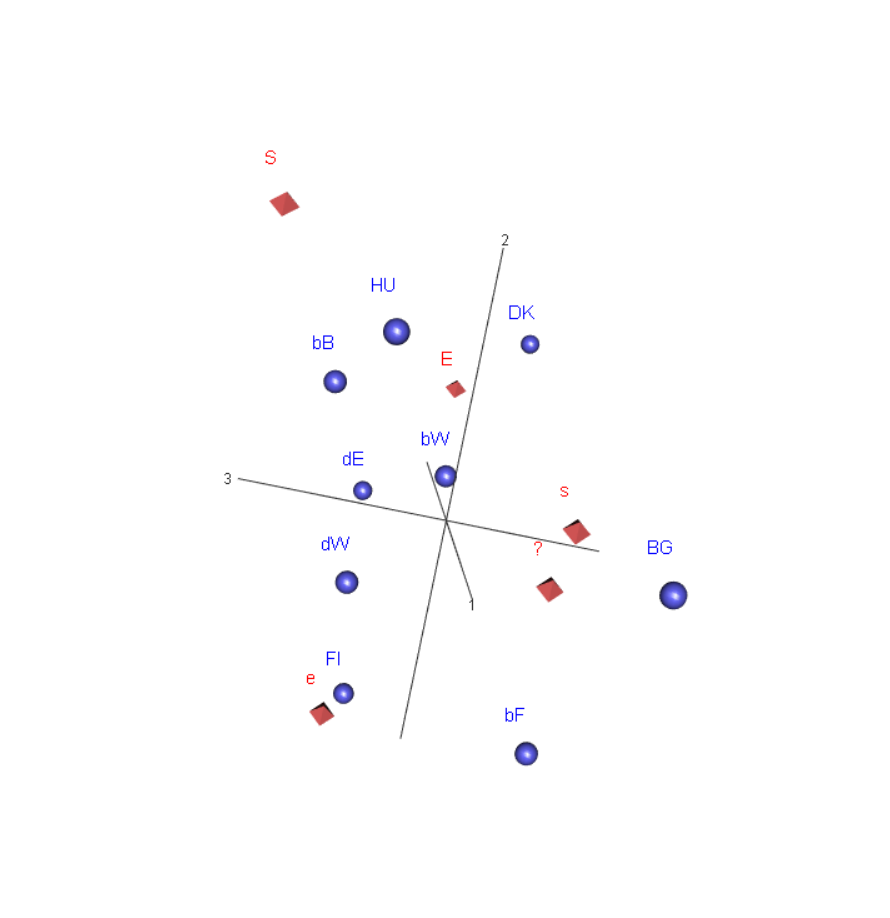
\includegraphics[width=0.9\linewidth]{img/3dSymMap_2} 

}

\caption{Saksan ja  Belgian aluejako - 3d-kuva2}\label{fig:3dklippi2}
\end{figure}

\hypertarget{yhteisvaikutusmuuttujat}{%
\chapter{Yhteisvaikutusmuuttujat}\label{yhteisvaikutusmuuttujat}}

\textbf{ks} ``Interactive coding''

\textbf{edit} Yksinkertaisin tapa ottaa muita muuttujia mukaan analyysiin.

\textbf{k} Kaksi yhteisvaikutusmuuttujaan (MG ``interactive coding''), sukupuoli ja
ikäluokka/kohortti ja tämän muuttujan yhdistäminen maa-muuttujaan.

\textbf{k} Poikkileikkausaineistossa vastaajaan ikä kuvaa sekä ikää että mitä erilaisimipia
sukupolvivaikutuksia. Ei voi oikein erottaa toisistaan. Vastaajat ovat elämänsä eri
vaiheissa kohdanneet lukuisia rajuja muutoksia toisen maailmansodan jälkeen. Nähtiin
jo edellisessä jaksossa!

Poikkileikkausaineistossa vastaajan ikä kertoo ikäluokan (kohortin), vastaajat ovat
kokeen esim. kaksi mullistusten vuotta elämänsä eri vaiheissa. Kaksin nuorinta ikäluokka
on ollut 1990 alle 14-vuotiaita ja vanhin ikäluokka yli 44-vuotiaita. Finannsikriisin
vuonna 2008 toiseksi nuorin ikäluokka on ollut 22-31 vuotiaita, ja kaksi vanhinta
yli 51-vuotiaita.

\hypertarget{ikuxe4-ja-sukupuoli}{%
\section{Ikä ja sukupuoli}\label{ikuxe4-ja-sukupuoli}}

\textbf{edit} Lyhyesti tämä, aineisto aggregoitu ikä- ja sukupuoliryhmiin.
\textbf{edit} Voi myös lisätä täydentävinä pisteinä ``peruskarttaan'', ei tehdä.

Ikäluokat ovat (1=15-25, 2 =26-35, 3=36-45, 4=46-55, 5=56-65, 6= 66 tai vanhempi).
Vuorovaikutusmuuttuja ga koodataan f1,\ldots, f6 ja m1,\ldots,m6. Muuttujien nimet
kannattaa pitää mahdollisimman lyhyinä.

Ikäjäkauma painottuu kaikissa maissa jonkinverran vanhempiin ikäluokkiin.
Nuorempien ikäluokkien osuus on (alle 26-vuotiaat ja alle 26-35 - vuotiaat)
varsinkin Bulgariassa (BG) ja Unkarissa (HU) pieni.

\textbf{k} Ikä- ja sukupuoliryhmät yli kaikkien maiden; profiilit keskiarvoja. Ei kovin
pätevää analyysiä, yleiskuva muuttujasta.

\begin{figure}

{\centering 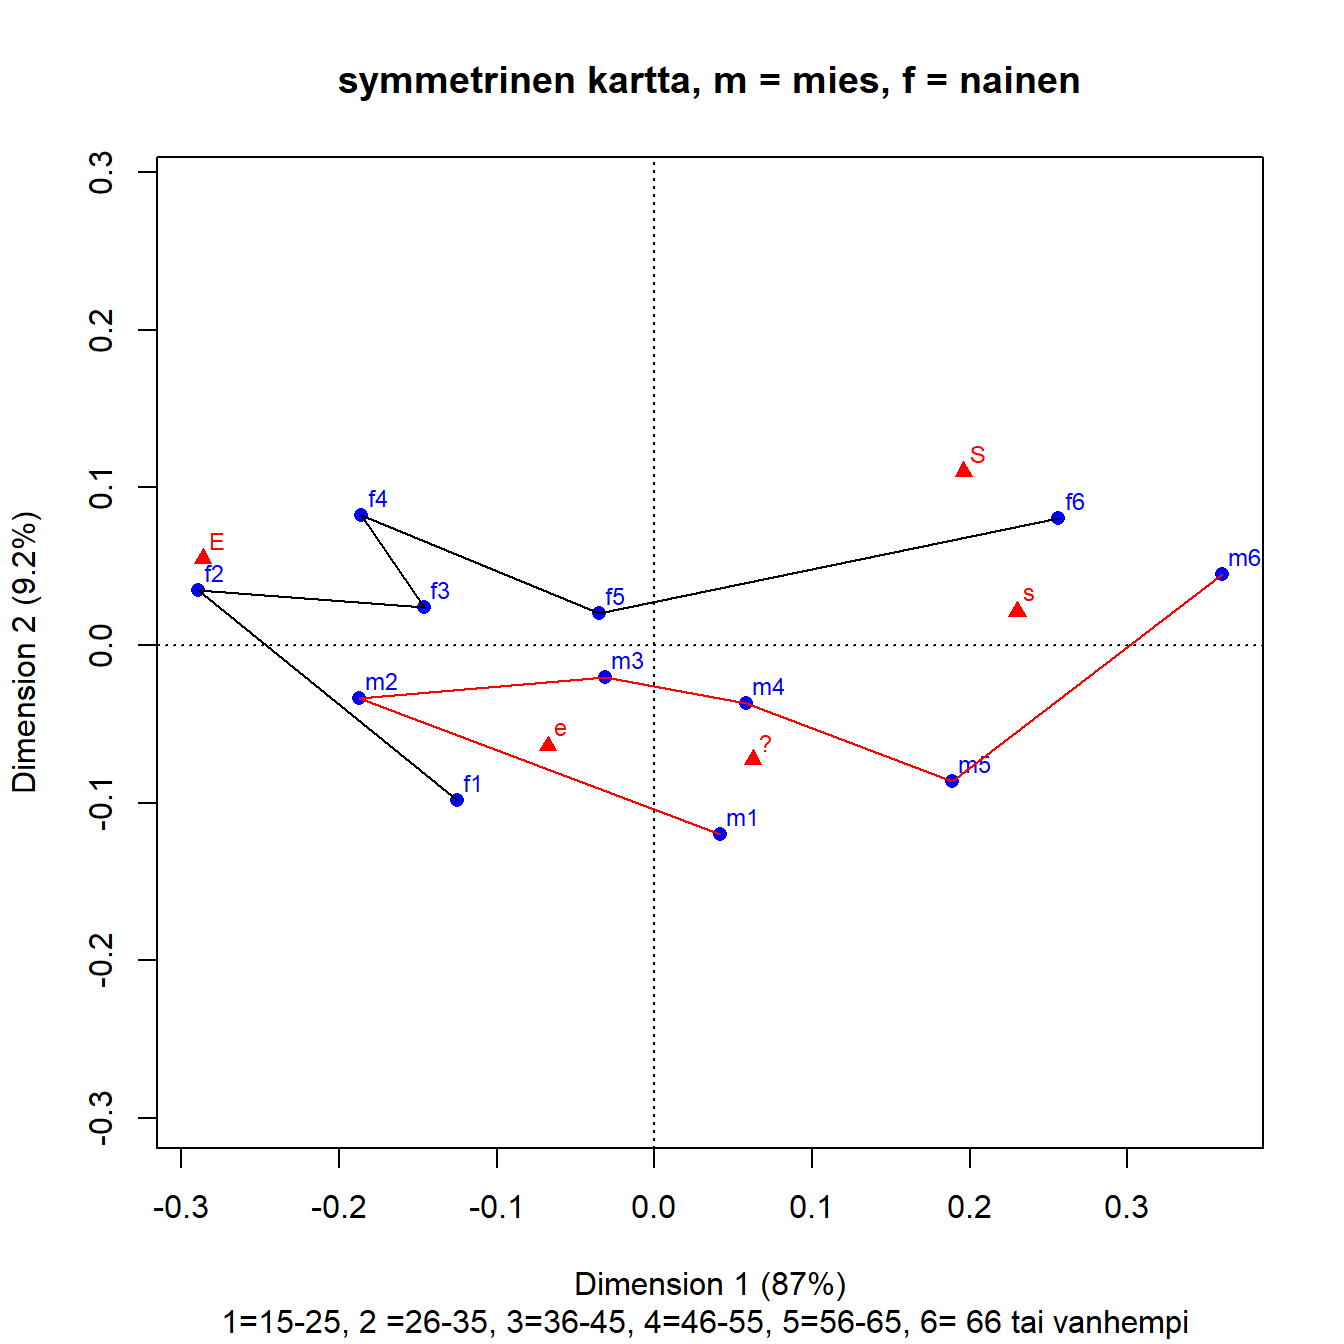
\includegraphics[width=0.9\linewidth]{JH_capaper_files/figure-latex/gaCA1map-1} 

}

\caption{Q1b: ikäluokka ja sukupuoli}\label{fig:gaCA1map}
\end{figure}

\begin{verbatim}
## 
## Principal inertias (eigenvalues):
## 
##  dim    value      %   cum%   scree plot               
##  1      0.037448  87.0  87.0  **********************   
##  2      0.003977   9.2  96.2  **                       
##  3      0.001041   2.4  98.6  *                        
##  4      0.000590   1.4 100.0                           
##         -------- -----                                 
##  Total: 0.043055 100.0                                 
## 
## 
## Rows:
##      name   mass  qlt  inr    k=1 cor ctr    k=2 cor ctr  
## 1  |   f1 |   60  990   36 | -125 614  25 |  -98 376 145 |
## 2  |   f2 |   83  997  163 | -289 983 185 |   35  14  25 |
## 3  |   f3 |   91  984   47 | -146 958  52 |   24  26  13 |
## 4  |   f4 |  101 1000   97 | -186 836  93 |   82 164 172 |
## 5  |   f5 |   98  879    4 |  -35 658   3 |   20 221  10 |
## 6  |   f6 |  100  951  176 |  256 866 175 |   80  85 162 |
## 7  |   m1 |   57  659   32 |   42  72   3 | -120 587 205 |
## 8  |   m2 |   66  977   57 | -187 946  62 |  -34  30  19 |
## 9  |   m3 |   78  457    5 |  -31 318   2 |  -20 139   8 |
## 10 |   m4 |   89  674   14 |   58 482   8 |  -37 192  30 |
## 11 |   m5 |   89  988   90 |  189 818  85 |  -86 170 166 |
## 12 |   m6 |   89  978  277 |  360 963 307 |   45  15  45 |
## 
## Columns:
##     name   mass  qlt  inr    k=1 cor ctr    k=2 cor ctr  
## 1 |    S |   99  915  128 |  196 695 102 |  110 220 304 |
## 2 |    s |  238  969  304 |  230 961 336 |   21   8  27 |
## 3 |      |  168  777   46 |   62 330  17 |  -73 447 223 |
## 4 |    e |  261  897   58 |  -68 473  32 |  -64 424 268 |
## 5 |    E |  234  997  464 | -286 962 513 |   55  35 177 |
\end{verbatim}

\textbf{k} Kommentteja Galkusta:
Aika yksiuloitteinen (87 prosenttia ensimmäisellä dimensiolla!). Data on
``as it is'', ei ole vakioitu ga-luokkien kokoja (massat max(f4 101), min (m1 57)).

Miten pitäisi tulkita ``oikealle kaatunut U - muoto'' miehillä ja naisilla?
Järjestys ei toimi, S s-sarakkeen vasemmalla puolella. Miehet konservatiivisempia,
mutta maltillisempia? Nuorin ikäluokka on poikkeava. Epävarmoja tai maltillisesti
e, sitten loikka vasemmalle ja sieltä konservatiiviseen suuntaa oikealle. Naisilla
poikkeama f3 - f4. VAnhimmat ikäluokat tiukemmin konservatiivisa (f6, m6). Jos
vertaa sukupuolten eroja samassa ikäluokassa, on aika samanlainen (miehet
konservatiivisia, naiset liberaaleja). Naisista vain vanhin ikäluokka oikealla,
miehistä nuorin ja kolme vanhinta.

Tulkinnassa muistettava, että ikäluokat yli maiden. Voi verrata sekä
edellisiin maa-vertailuihin että maan, ikäluokan ja sukupuolen yhteisvaikutusmuuttujan
tuloksiin. MG tutkailee eri kysymyksellä tätä samaa asiaa, ja havaitsee että
(a) maiden erot suuria ja sukupuolten pieniä (b) naiset liberaalimpia kuin miehet.
** Viite?**

Numeeriset tulokset: nuorimpien miesten (qlt 659) ja erityisesti
keski-ikäisten miestén m3 (qlt 457) pisteet huonosti esitetty kartalla. Tulkitaan
myös cor ja ctr, riveille ja sarakkeille.

\hypertarget{ikuxe4-sukupuoli-ja-maa}{%
\section{Ikä, sukupuoli ja maa}\label{ikuxe4-sukupuoli-ja-maa}}

\begin{Shaded}
\begin{Highlighting}[]
\NormalTok{ISSP2012esim1b.dat <-}\StringTok{ }\KeywordTok{mutate}\NormalTok{(ISSP2012esim1b.dat,}
                             \DataTypeTok{maaga =} \KeywordTok{paste}\NormalTok{(maa, ga, }\DataTypeTok{sep =} \StringTok{""}\NormalTok{))}

\CommentTok{# tarkistus, muunnos ok}
\CommentTok{# ISSP2012esim1b.dat %>% tableX(maa, maaga)}
\CommentTok{# head(ISSP2012esim2.dat)}
\CommentTok{# str(ISSP2012esim2.dat)}
\end{Highlighting}
\end{Shaded}

\textbf{edit} Yksi vaikeaselkoinen kartta täynnä pisteitä, tihrustellaan.

\begin{figure}

{\centering 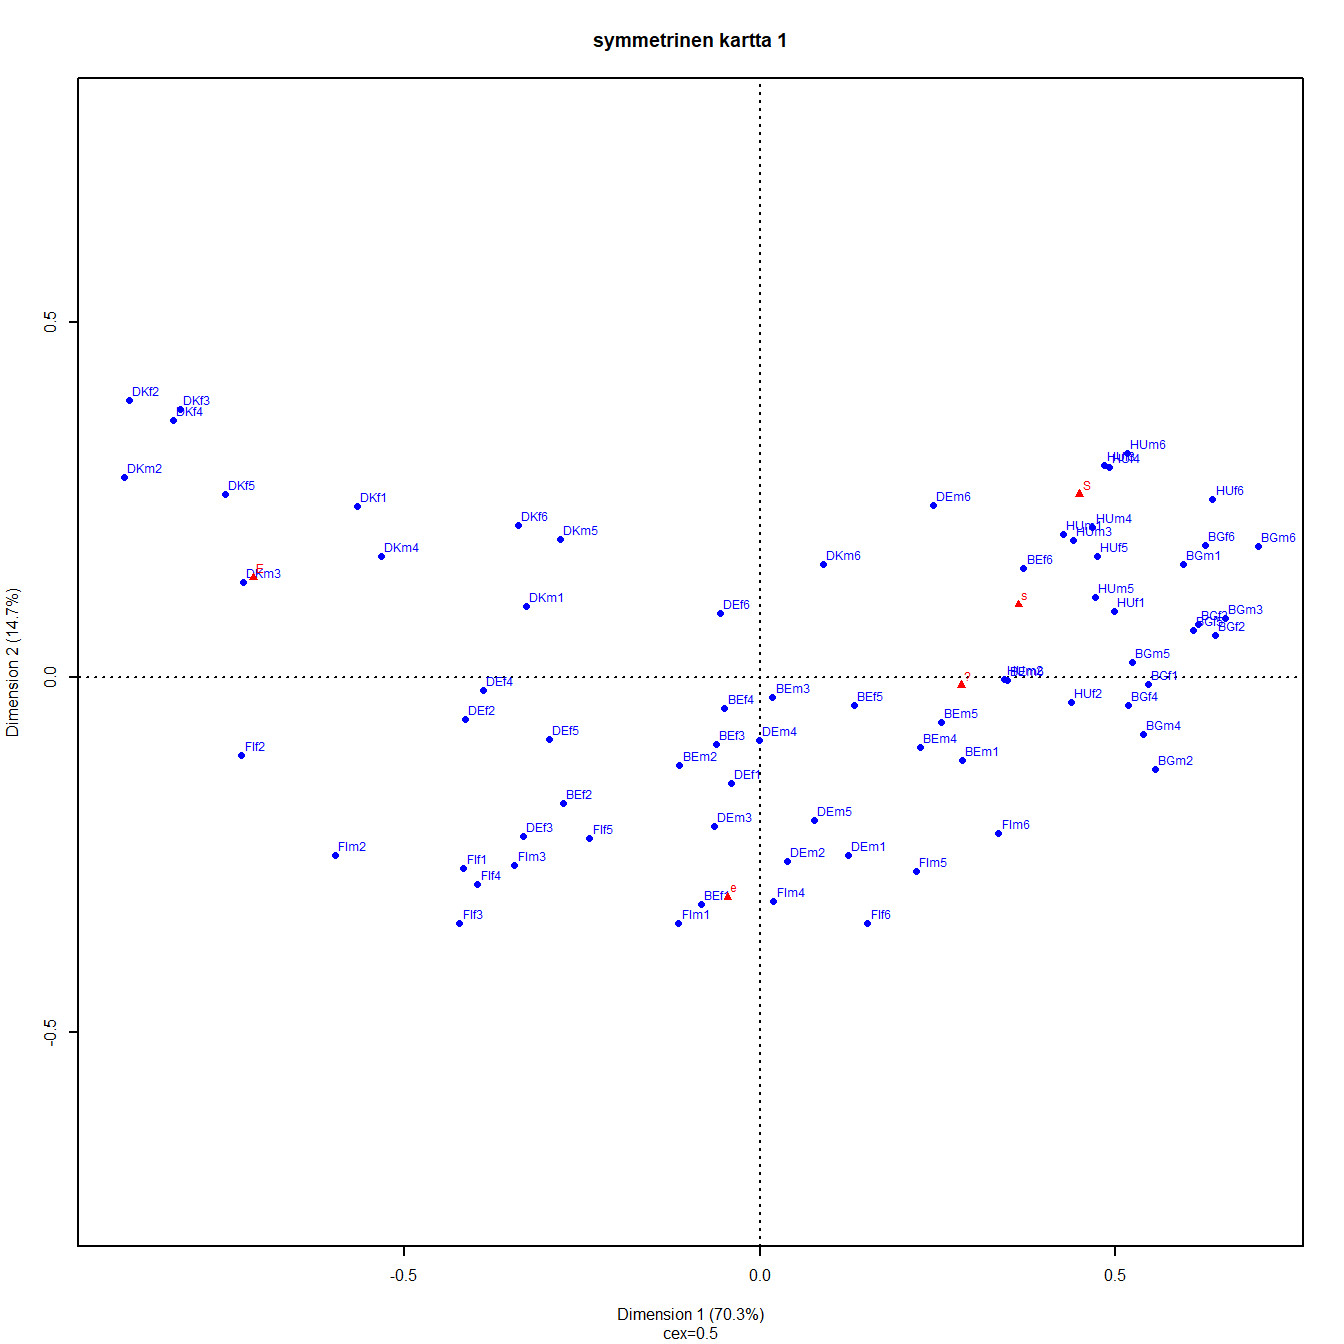
\includegraphics[width=0.9\linewidth]{JH_capaper_files/figure-latex/maagaCA1map1-1} 

}

\caption{Q1b: ikäluokka ja sukupuoli maittain}\label{fig:maagaCA1map1}
\end{figure}

\begin{Shaded}
\begin{Highlighting}[]
\CommentTok{# Vilkaistaan numeerisia tuloksia, kopioidaan tekstiin jos on tarpeellista}

\KeywordTok{print}\NormalTok{(maagaCA1)}
\end{Highlighting}
\end{Shaded}

\begin{verbatim}
## 
##  Principal inertias (eigenvalues):
##            1        2        3        4       
## Value      0.184895 0.038751 0.024006 0.015502
## Percentage 70.26%   14.73%   9.12%    5.89%   
## 
## 
##  Rows:
##              BEf1      BEf2      BEf3      BEf4      BEf5     BEf6      BEm1
## Mass     0.014245  0.024315  0.021368  0.024438  0.022842 0.022719  0.011298
## ChiDist  0.401386  0.344292  0.199783  0.164967  0.240455 0.439918  0.469422
## Inertia  0.002295  0.002882  0.000853  0.000665  0.001321 0.004397  0.002490
## Dim. 1  -0.192908 -0.645510 -0.144265 -0.116669  0.308332 0.862093  0.661555
## Dim. 2  -1.625273 -0.897934 -0.480404 -0.223840 -0.203533 0.778887 -0.592620
##              BEm2      BEm3      BEm4      BEm5      BEm6      BGf1     BGf2
## Mass     0.016579  0.019894  0.021614  0.022350  0.025543  0.004912 0.007860
## ChiDist  0.276047  0.102584  0.250249  0.308070  0.392168  0.751086 0.693373
## Inertia  0.001263  0.000209  0.001354  0.002121  0.003928  0.002771 0.003779
## Dim. 1  -0.263692  0.040639  0.524364  0.593355  0.809427  1.272436 1.489306
## Dim. 2  -0.632522 -0.146484 -0.498708 -0.319489 -0.023713 -0.047377 0.300670
##             BGf3      BGf4     BGf5     BGf6     BGm1      BGm2     BGm3
## Mass    0.011544  0.010438 0.014000 0.018298 0.004544  0.006263 0.007982
## ChiDist 0.688564  0.538800 0.653467 0.681719 0.636676  0.627620 0.784126
## Inertia 0.005473  0.003030 0.005978 0.008504 0.001842  0.002467 0.004908
## Dim. 1  1.435410  1.206311 1.417403 1.458638 1.387090  1.295443 1.523242
## Dim. 2  0.380068 -0.199915 0.334139 0.942930 0.805581 -0.659426 0.420697
##              BGm4     BGm5     BGm6      DEf1      DEf2      DEf3      DEf4
## Mass     0.007737 0.010316 0.009210  0.012526  0.014737  0.018666  0.022842
## ChiDist  0.622138 0.529671 0.871456  0.237411  0.432439  0.436045  0.393174
## Inertia  0.002995 0.002894 0.006995  0.000706  0.002756  0.003549  0.003531
## Dim. 1   1.256092 1.217661 1.630600 -0.094359 -0.964139 -0.773449 -0.906287
## Dim. 2  -0.411230 0.106062 0.934896 -0.758320 -0.302962 -1.138600 -0.093489
##              DEf5      DEf6      DEm1      DEm2      DEm3      DEm4      DEm5
## Mass     0.016579  0.022719  0.012649  0.012649  0.014982  0.021122  0.018789
## ChiDist  0.337893  0.312735  0.292550  0.298896  0.255414  0.239923  0.277383
## Inertia  0.001893  0.002222  0.001083  0.001130  0.000977  0.001216  0.001446
## Dim. 1  -0.690438 -0.131007  0.288893  0.088588 -0.149437 -0.002440  0.176330
## Dim. 2  -0.443502  0.459553 -1.271559 -1.314308 -1.064830 -0.450858 -1.024467
##             DEm6      DKf1      DKf2      DKf3      DKf4      DKf5      DKf6
## Mass    0.022228  0.010193  0.013509  0.016701  0.017930  0.015719  0.012158
## ChiDist 0.373055  0.618958  0.974207  0.915861  0.912001  0.796636  0.447079
## Inertia 0.003093  0.003905  0.012821  0.014009  0.014913  0.009976  0.002430
## Dim. 1  0.566840 -1.318547 -2.065738 -1.896750 -1.920212 -1.751477 -0.791121
## Dim. 2  1.230963  1.224334  1.977279  1.917537  1.838583  1.309298  1.085880
##              DKm1      DKm2      DKm3      DKm4      DKm5     DKm6      FIf1
## Mass     0.015228  0.012649  0.013386  0.015351  0.013017 0.014614  0.011544
## ChiDist  0.347520  0.944015  0.746858  0.577246  0.425435 0.305128  0.501340
## Inertia  0.001839  0.011272  0.007467  0.005115  0.002356 0.001361  0.002901
## Dim. 1  -0.766023 -2.082325 -1.692619 -1.241148 -0.652736 0.206674 -0.970679
## Dim. 2   0.508647  1.430786  0.679314  0.861313  0.985212 0.805173 -1.364560
##              FIf2      FIf3      FIf4      FIf5      FIf6      FIm1      FIm2
## Mass     0.011666  0.011544  0.014491  0.017438  0.011175  0.007123  0.008719
## ChiDist  0.766236  0.551096  0.495644  0.338299  0.414096  0.411753  0.655833
## Inertia  0.006850  0.003506  0.003560  0.001996  0.001916  0.001208  0.003750
## Dim. 1  -1.696716 -0.984276 -0.924988 -0.557306  0.352194 -0.266716 -1.390905
## Dim. 2  -0.559707 -1.756948 -1.483475 -1.152838 -1.760989 -1.762100 -1.272164
##              FIm3      FIm4      FIm5      FIm6     HUf1      HUf2     HUf3
## Mass     0.008719  0.012895  0.011789  0.009210 0.006631  0.010561 0.011666
## ChiDist  0.435509  0.346131  0.408938  0.420689 0.596829  0.528993 0.632471
## Inertia  0.001654  0.001545  0.001972  0.001630 0.002362  0.002955 0.004667
## Dim. 1  -0.803330  0.044427  0.510847  0.780773 1.159811  1.018217 1.125535
## Dim. 2  -1.344478 -1.605387 -1.387245 -1.118123 0.474792 -0.177617 1.513996
##             HUf4     HUf5     HUf6     HUm1      HUm2     HUm3     HUm4
## Mass    0.011175 0.011544 0.012772 0.006017  0.009210 0.012649 0.009824
## ChiDist 0.654467 0.546586 0.835835 0.487239  0.557409 0.492095 0.513571
## Inertia 0.004787 0.003449 0.008923 0.001429  0.002862 0.003063 0.002591
## Dim. 1  1.142602 1.103056 1.481505 0.991480  0.799636 1.025502 1.088005
## Dim. 2  1.501687 0.864556 1.274631 1.019905 -0.011945 0.980496 1.073058
##             HUm5     HUm6
## Mass    0.012526 0.007860
## ChiDist 0.499875 0.710900
## Inertia 0.003130 0.003972
## Dim. 1  1.097228 1.202188
## Dim. 2  0.572470 1.601967
## 
## 
##  Columns:
##                S        s         ?         e         E
## Mass    0.099472 0.237627  0.167874  0.260960  0.234066
## ChiDist 0.641178 0.439383  0.388506  0.322679  0.727480
## Inertia 0.040894 0.045876  0.025338  0.027172  0.123874
## Dim. 1  1.045509 0.846873  0.660109 -0.105643 -1.659727
## Dim. 2  1.310121 0.516896 -0.057407 -1.573335  0.713757
\end{verbatim}

\begin{Shaded}
\begin{Highlighting}[]
\KeywordTok{summary}\NormalTok{(maagaCA1)}
\end{Highlighting}
\end{Shaded}

\begin{verbatim}
## 
## Principal inertias (eigenvalues):
## 
##  dim    value      %   cum%   scree plot               
##  1      0.184895  70.3  70.3  ******************       
##  2      0.038751  14.7  85.0  ****                     
##  3      0.024006   9.1  94.1  **                       
##  4      0.015502   5.9 100.0  *                        
##         -------- -----                                 
##  Total: 0.263154 100.0                                 
## 
## 
## Rows:
##      name   mass  qlt  inr    k=1 cor ctr    k=2 cor ctr  
## 1  | BEf1 |   14  678    9 |  -83  43   1 | -320 635  38 |
## 2  | BEf2 |   24  914   11 | -278 650  10 | -177 264  20 |
## 3  | BEf3 |   21  320    3 |  -62  96   0 |  -95 224   5 |
## 4  | BEf4 |   24  164    3 |  -50  92   0 |  -44  71   1 |
## 5  | BEf5 |   23  332    5 |  133 304   2 |  -40  28   1 |
## 6  | BEf6 |   23  832   17 |  371 710  17 |  153 121  14 |
## 7  | BEm1 |   11  429    9 |  284 367   5 | -117  62   4 |
## 8  | BEm2 |   17  372    5 | -113 169   1 | -125 203   7 |
## 9  | BEm3 |   20  108    1 |   17  29   0 |  -29  79   0 |
## 10 | BEm4 |   22  966    5 |  225 812   6 |  -98 154   5 |
## 11 | BEm5 |   22  728    8 |  255 686   8 |  -63  42   2 |
## 12 | BEm6 |   26  788   15 |  348 788  17 |   -5   0   0 |
## 13 | BGf1 |    5  531   11 |  547 531   8 |   -9   0   0 |
## 14 | BGf2 |    8  860   14 |  640 853  17 |   59   7   1 |
## 15 | BGf3 |   12  815   21 |  617 804  24 |   75  12   2 |
## 16 | BGf4 |   10  932   12 |  519 927  15 |  -39   5   0 |
## 17 | BGf5 |   14  880   23 |  609 870  28 |   66  10   2 |
## 18 | BGf6 |   18  921   32 |  627 846  39 |  186  74  16 |
## 19 | BGm1 |    5  940    7 |  596 878   9 |  159  62   3 |
## 20 | BGm2 |    6  830    9 |  557 788  11 | -130  43   3 |
## 21 | BGm3 |    8  709   19 |  655 698  19 |   83  11   1 |
## 22 | BGm4 |    8  771   11 |  540 754  12 |  -81  17   1 |
## 23 | BGm5 |   10  979   11 |  524 977  15 |   21   2   0 |
## 24 | BGm6 |    9  692   27 |  701 647  24 |  184  45   8 |
## 25 | DEf1 |   13  425    3 |  -41  29   0 | -149 395   7 |
## 26 | DEf2 |   15  938   10 | -415 919  14 |  -60  19   1 |
## 27 | DEf3 |   19  846   13 | -333 582  11 | -224 264  24 |
## 28 | DEf4 |   23  985   13 | -390 982  19 |  -18   2   0 |
## 29 | DEf5 |   17  839    7 | -297 772   8 |  -87  67   3 |
## 30 | DEf6 |   23  116    8 |  -56  32   0 |   90  84   5 |
## 31 | DEm1 |   13  912    4 |  124 180   1 | -250 732  20 |
## 32 | DEm2 |   13  766    4 |   38  16   0 | -259 749  22 |
## 33 | DEm3 |   15  737    4 |  -64  63   0 | -210 674  17 |
## 34 | DEm4 |   21  137    5 |   -1   0   0 |  -89 137   4 |
## 35 | DEm5 |   19  603    5 |   76  75   1 | -202 529  20 |
## 36 | DEm6 |   22  849   12 |  244 427   7 |  242 422  34 |
## 37 | DKf1 |   10  991   15 | -567 839  18 |  241 152  15 |
## 38 | DKf2 |   14  991   49 | -888 831  58 |  389 160  53 |
## 39 | DKf3 |   17  963   53 | -816 793  60 |  377 170  61 |
## 40 | DKf4 |   18  977   57 | -826 820  66 |  362 157  61 |
## 41 | DKf5 |   16  998   38 | -753 894  48 |  258 105  27 |
## 42 | DKf6 |   12  808    9 | -340 579   8 |  214 229  14 |
## 43 | DKm1 |   15  981    7 | -329 898   9 |  100  83   4 |
## 44 | DKm2 |   13  989   43 | -895 900  55 |  282  89  26 |
## 45 | DKm3 |   13  982   28 | -728 950  38 |  134  32   6 |
## 46 | DKm4 |   15  941   19 | -534 855  24 |  170  86  11 |
## 47 | DKm5 |   13  643    9 | -281 435   6 |  194 208  13 |
## 48 | DKm6 |   15  355    5 |   89  85   1 |  158 270   9 |
## 49 | FIf1 |   12  980   11 | -417 693  11 | -269 287  21 |
## 50 | FIf2 |   12  927   26 | -730 907  34 | -110  21   4 |
## 51 | FIf3 |   12  984   13 | -423 590  11 | -346 394  36 |
## 52 | FIf4 |   14  991   14 | -398 644  12 | -292 347  32 |
## 53 | FIf5 |   17  952    8 | -240 502   5 | -227 450  23 |
## 54 | FIf6 |   11  835    7 |  151 134   1 | -347 701  35 |
## 55 | FIm1 |    7  787    5 | -115  78   1 | -347 710  22 |
## 56 | FIm2 |    9  977   14 | -598 832  17 | -250 146  14 |
## 57 | FIm3 |    9  998    6 | -345 629   6 | -265 369  16 |
## 58 | FIm4 |   13  837    6 |   19   3   0 | -316 834  33 |
## 59 | FIm5 |   12  734    7 |  220 289   3 | -273 446  23 |
## 60 | FIm6 |    9  911    6 |  336 637   6 | -220 274  12 |
## 61 | HUf1 |    7  723    9 |  499 698   9 |   93  25   1 |
## 62 | HUf2 |   11  689   11 |  438 685  11 |  -35   4   0 |
## 63 | HUf3 |   12  808   18 |  484 586  15 |  298 222  27 |
## 64 | HUf4 |   11  768   18 |  491 564  15 |  296 204  25 |
## 65 | HUf5 |   12  850   13 |  474 753  14 |  170  97   9 |
## 66 | HUf6 |   13  671   34 |  637 581  28 |  251  90  21 |
## 67 | HUm1 |    6  935    5 |  426 766   6 |  201 170   6 |
## 68 | HUm2 |    9  381   11 |  344 381   6 |   -2   0   0 |
## 69 | HUm3 |   13  957   12 |  441 803  13 |  193 154  12 |
## 70 | HUm4 |   10  999   10 |  468 830  12 |  211 169  11 |
## 71 | HUm5 |   13  942   12 |  472 891  15 |  113  51   4 |
## 72 | HUm6 |    8  726   15 |  517 529  11 |  315 197  20 |
## 
## Columns:
##     name   mass  qlt  inr    k=1 cor ctr    k=2 cor ctr  
## 1 |    S |   99  653  155 |  450 492 109 |  258 162 171 |
## 2 |    s |  238  741  174 |  364 687 170 |  102  54  63 |
## 3 |      |  168  535   96 |  284 534  73 |  -11   1   1 |
## 4 |    e |  261  941  103 |  -45  20   3 | -310 921 646 |
## 5 |    E |  234 1000  471 | -714 962 645 |  141  37 119 |
\end{verbatim}

\hypertarget{stabiilisuus}{%
\section{Stabiilisuus}\label{stabiilisuus}}

\textbf{k} Stabiilius - teorialiitteessä laajemmin mutta tässä lyhyt vilkaisu.
Taulukko alkaa harveta, edellä kerrottiin että aineisto painottuu kaikissa maissa
vanhempiin ikäluokkiin.

\textbf{yksinkertainen tarkistus?} Löytyykö riviproviileja joilla pieni massa ja suuri
kontribuutio? Ei löydy (Galkussa tuloksia), mutta jo kuvan tukkoisuus vaatii
luokkien yhdistelyä. Aika työlästä!

\hypertarget{osajoukon-korrespondenssianalyysi}{%
\chapter{Osajoukon korrespondenssianalyysi}\label{osajoukon-korrespondenssianalyysi}}

\textbf{k} Osajoukon korrespondenssianalyysin tarve: kuvat menevät tukkoon. Kun muuttujia
on paljon kartat ovat täynnä pisteitä ja niitä on vaikea lukea. Usein myös havaitaan,
että ratkaisun päädimensiot kertovat ylllätyksettömän ilmeisen tarinan, ja
kiinnostavammat yhteydet ovat piilossa ylemmissä dimensioissa (MG ja Pardo, ``Vihreä
kirja'' ss. 198).

\textbf{k} Teoreettinen idea: inertian dekomoponointi (taas). Lasketaan ensin
ca-ratkaisu ja rajataan aineisto. Yksinkertainen toteuttaa. Massat ja reunajakaumat
säilyvä, ja siksi aineiston (``pilven'') kokonaisinertia voidaan jakaa osiin
osajoukkojen inertiaksi. Uusia yhteyksiä näkyviin, tarkempi kuva datasta.

Kuvan tukkoisuuteen voi toki vaikuttaa muillakin keinoilla. Muuttujien arvoja voi
yhdistellä, kuvasta voi jättää pois pisteitä joiden kontribuutio on pieni tai kuvaa
voi yksinkertaisesti suurentaa analyysivaiheessa näytöllä.

Kuva-aluetta voi myös rajata johonkin osaan kuvaa. Kaikki pisteet ovat kuitenkin
mukana määräämässä ratkaisun geometriaa.

Rivejä tai sarakkeita voi myös muuttaa passiivisiksi, mutta silloin ei saavuteta
käytännöllistä inertian dekomponointi-ominaisuutta. MCA-jaksossa osajoukon
analysointi on pääasia ja mahdollisia vaihtoehtoja käsitellään hieman lisää.

Lähteet MG ja Prado (2006)\citep{RefWorks:doc:5a857a44e4b0ed2d44664d87},
``vihreä kirja'' \citep{RefWorks:doc:5ab76b43e4b003f4468d1f07},
CAiP \citep{RefWorks:doc:5a857a43e4b0ed2d44664d78}.

\textbf{k} Simple CA subset

\textbf{k1} Täydentävät pisteet voi ottaa mukaan jos ne eivät ole rajatusta ``pilvestä''.
Esim. rivien osajoukon analyysiin voi ottaa sarakepisteitä täydeäntvinä pisteinä
normaalisti. Osajoukon profiilit muuttuvat, niiden summa ei enään ole yksi,
barysentristä ominaisuutta ei voi suoraan käyttää täydentävien rivipisteiden
koordinaattien laskemiseen.

\textbf{k2} Kuvien luettavuus ja pistekoko, hankala juttu

\begin{figure}

{\centering 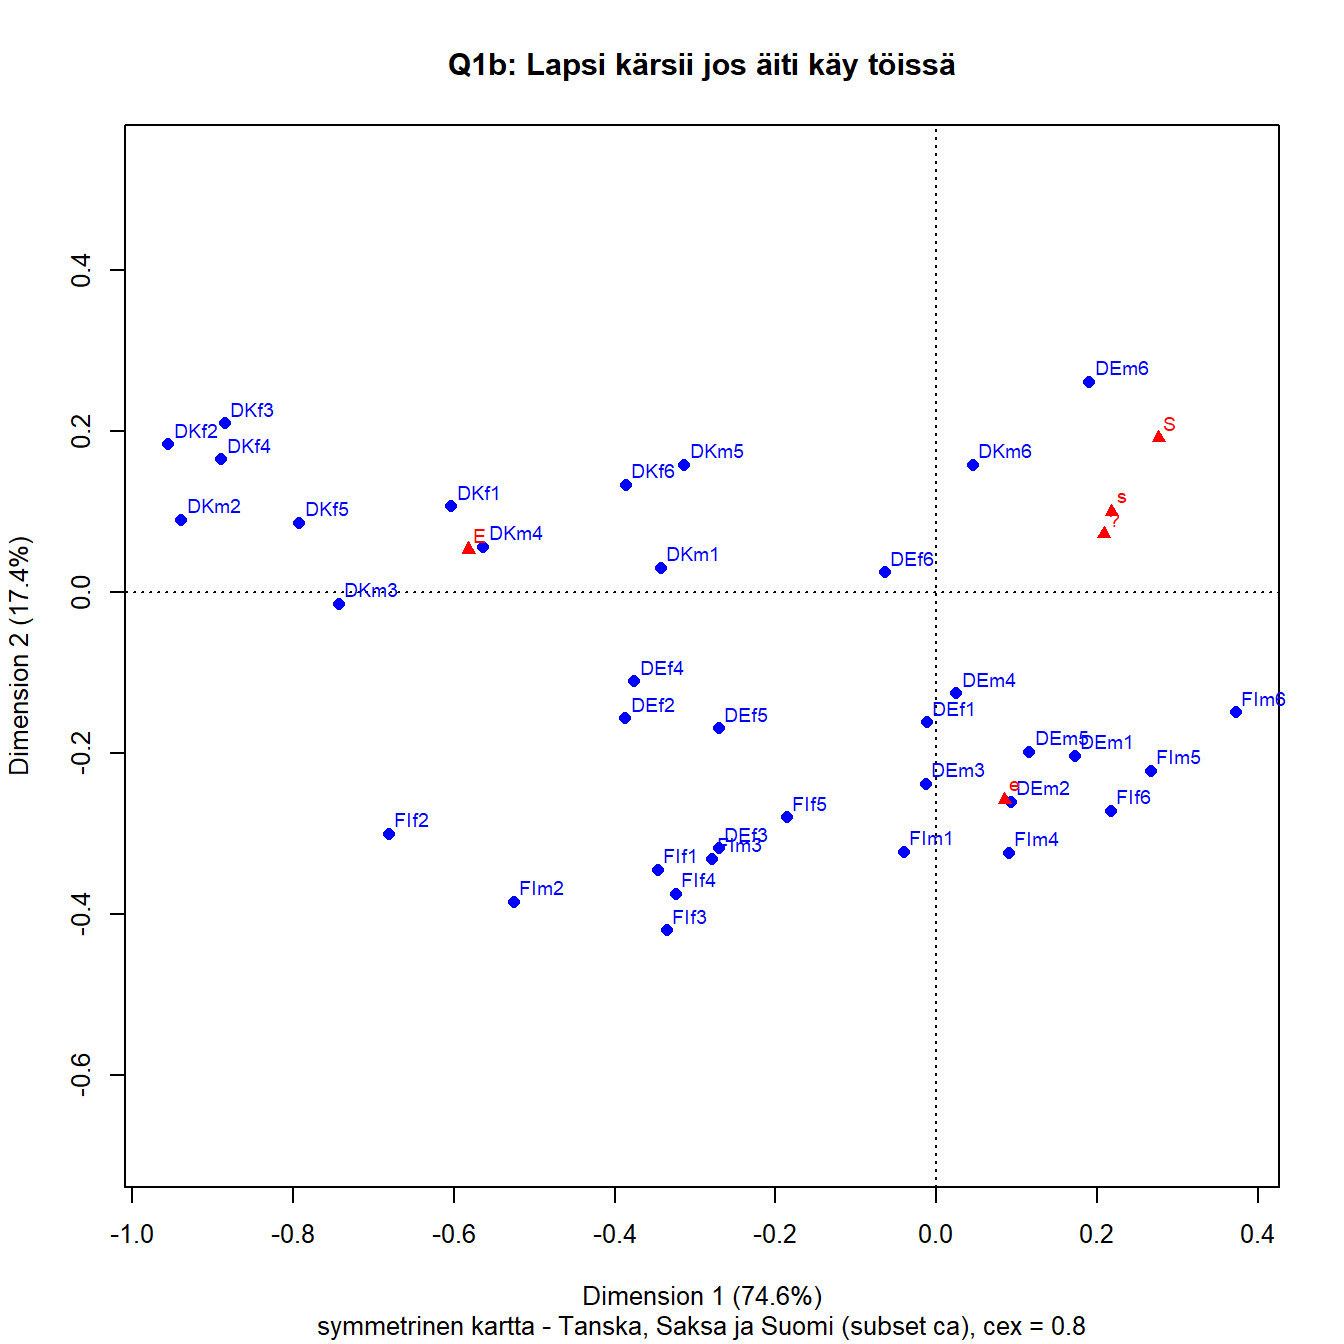
\includegraphics[width=0.9\linewidth]{JH_capaper_files/figure-latex/maagaCA2sub2map1-1} 

}

\caption{Ikä, sukupuoli ja maa:Tanska-Saksa-Suomi}\label{fig:maagaCA2sub2map1}
\end{figure}

\begin{figure}

{\centering 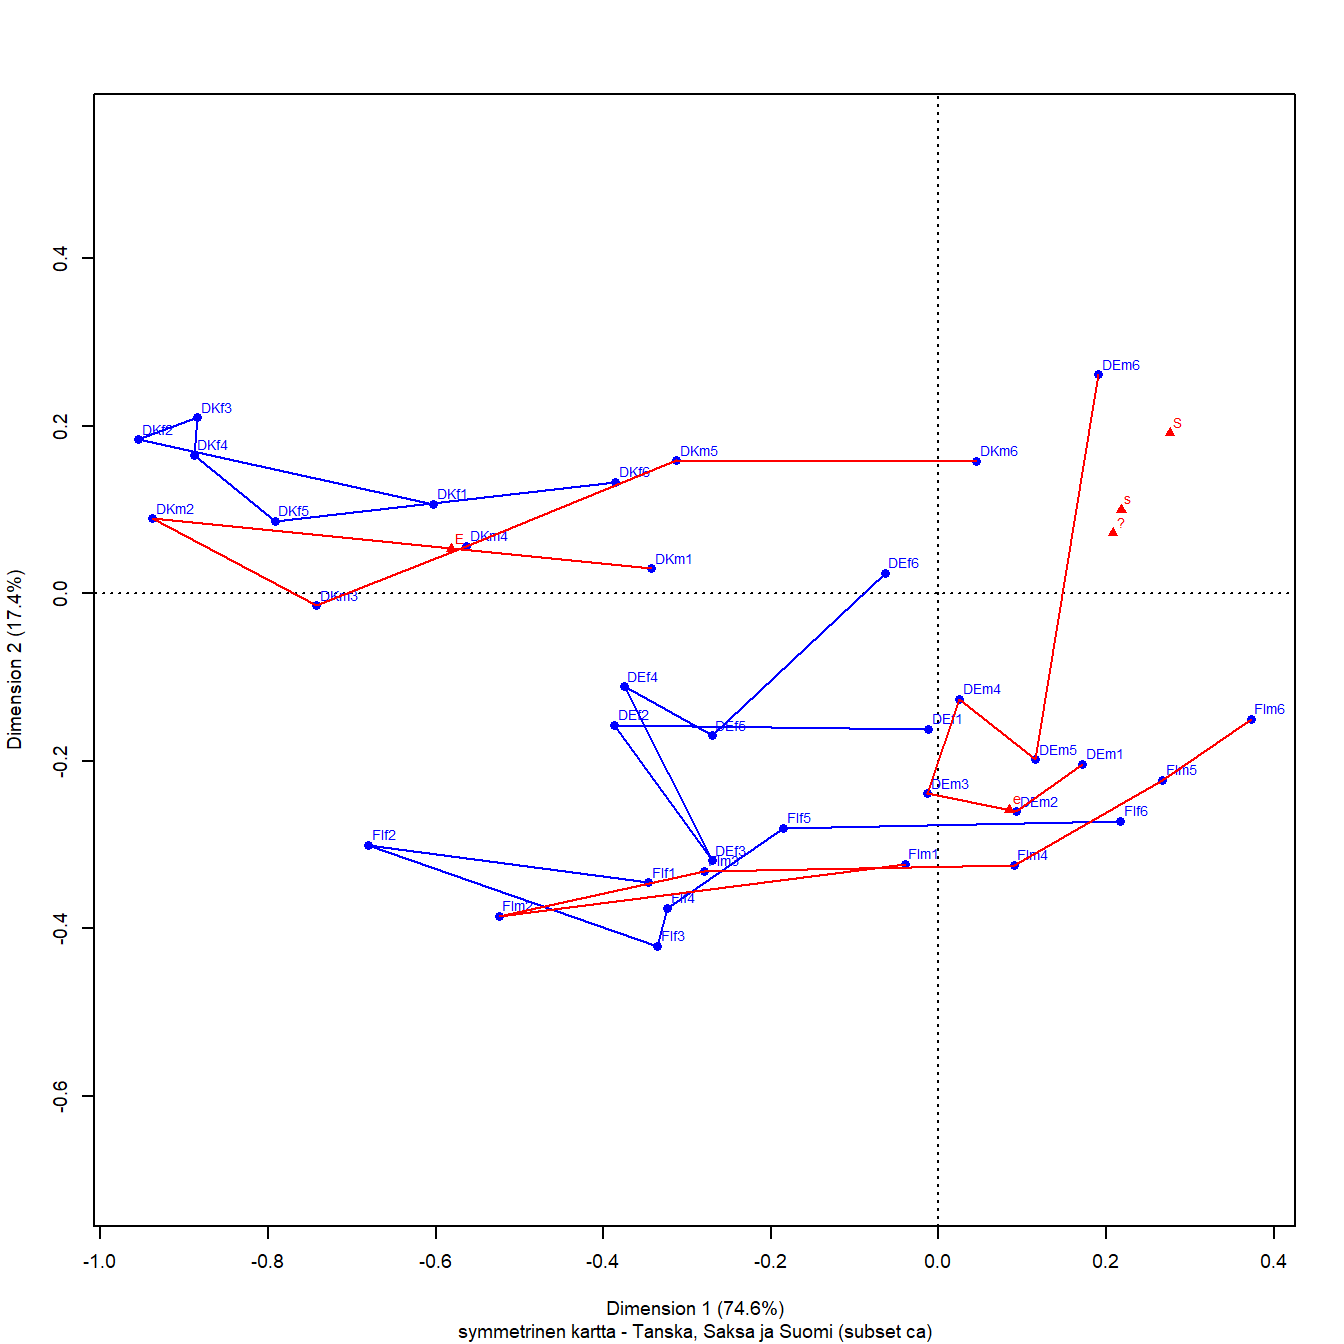
\includegraphics[width=0.9\linewidth]{JH_capaper_files/figure-latex/maagaCA2sub2map2-1} 

}

\caption{Ikä, sukupuoli ja maa:Tanska-Saksa-Suomi}\label{fig:maagaCA2sub2map2}
\end{figure}

\begin{figure}

{\centering 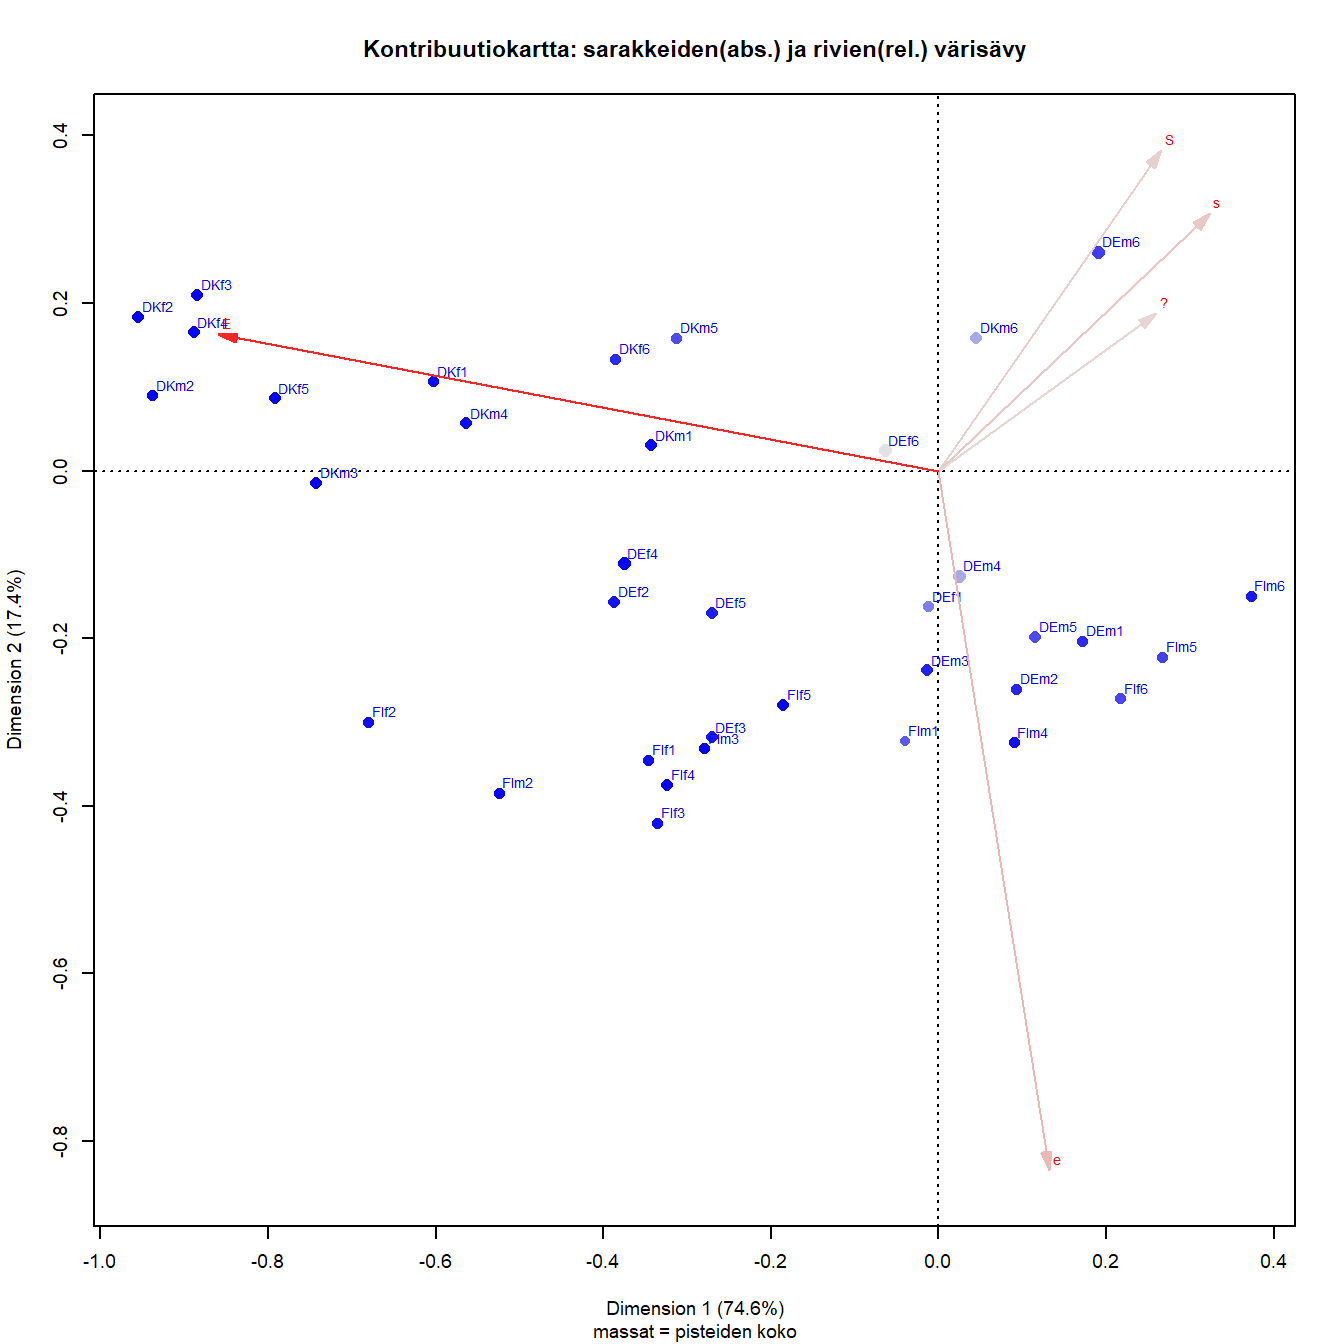
\includegraphics[width=0.9\linewidth]{JH_capaper_files/figure-latex/maagaCA2sub2map3-1} 

}

\caption{Ikä, sukupuoli ja maa:Tanska-Saksa-Suomi}\label{fig:maagaCA2sub2map3}
\end{figure}

\begin{verbatim}
## 
## Principal inertias (eigenvalues):
## 
##  dim    value      %   cum%   scree plot               
##  1      0.107090  74.6  74.6  *******************      
##  2      0.024985  17.4  92.0  ****                     
##  3      0.006594   4.6  96.6  *                        
##  4      0.004882   3.4 100.0  *                        
##         -------- -----                                 
##  Total: 0.143551 100.0                                 
## 
## 
## Rows:
##      name   mass  qlt  inr    k=1 cor ctr    k=2 cor ctr  
## 1  | DEf1 |   13  467    5 |  -12   3   0 | -162 464  13 |
## 2  | DEf2 |   15  930   19 | -387 799  21 | -157 131  14 |
## 3  | DEf3 |   19  919   25 | -271 385  13 | -318 533  76 |
## 4  | DEf4 |   23  993   25 | -376 913  30 | -111  80  11 |
## 5  | DEf5 |   17  893   13 | -271 641  11 | -169 252  19 |
## 6  | DEf6 |   23   48   15 |  -64  42   1 |   24   6   1 |
## 7  | DEm1 |   13  827    8 |  172 345   3 | -203 482  21 |
## 8  | DEm2 |   13  855    8 |   93  96   1 | -260 759  34 |
## 9  | DEm3 |   15  874    7 |  -13   3   0 | -238 871  34 |
## 10 | DEm4 |   21  285    8 |   25  11   0 | -126 274  13 |
## 11 | DEm5 |   19  684   10 |  116 174   2 | -198 510  30 |
## 12 | DEm6 |   22  750   22 |  190 260   8 |  261 490  61 |
## 13 | DKf1 |   10  979   27 | -603 949  35 |  107  30   5 |
## 14 | DKf2 |   14  996   89 | -955 960 115 |  184  36  18 |
## 15 | DKf3 |   17  985   98 | -885 933 122 |  210  53  29 |
## 16 | DKf4 |   18  983  104 | -889 950 132 |  165  33  20 |
## 17 | DKf5 |   16 1000   69 | -792 988  92 |   86  12   5 |
## 18 | DKf6 |   12  834   17 | -386 745  17 |  133  89   9 |
## 19 | DKm1 |   15  978   13 | -342 971  17 |   30   7   1 |
## 20 | DKm2 |   13  997   79 | -938 988 104 |   90   9   4 |
## 21 | DKm3 |   13  989   52 | -743 989  69 |  -14   0   0 |
## 22 | DKm4 |   15  962   36 | -563 952  45 |   57  10   2 |
## 23 | DKm5 |   13  682   16 | -314 543  12 |  159 139  13 |
## 24 | DKm6 |   15  291    9 |   45  22   0 |  158 269  15 |
## 25 | FIf1 |   12  951   20 | -346 478  13 | -345 474  55 |
## 26 | FIf2 |   12  941   48 | -680 788  50 | -300 153  42 |
## 27 | FIf3 |   12  952   24 | -335 370  12 | -420 582  82 |
## 28 | FIf4 |   14  999   25 | -323 426  14 | -375 573  82 |
## 29 | FIf5 |   17  982   14 | -185 299   6 | -280 683  55 |
## 30 | FIf6 |   11  704   13 |  217 274   5 | -271 430  33 |
## 31 | FIm1 |    7  624    8 |  -40  10   0 | -323 614  30 |
## 32 | FIm2 |    9  984   26 | -525 640  22 | -385 344  52 |
## 33 | FIm3 |    9  990   12 | -279 412   6 | -331 578  38 |
## 34 | FIm4 |   13  944   11 |   90  67   1 | -324 877  54 |
## 35 | FIm5 |   12  722   14 |  267 426   8 | -222 295  23 |
## 36 | FIm6 |    9  911   11 |  373 785  12 | -150 126   8 |
## 
## Columns:
##     name   mass  qlt  inr    k=1 cor ctr    k=2 cor ctr  
## 1 |    S |   99  731  107 |  276 493  71 |  192 238 147 |
## 2 |    s |  238  832  114 |  218 688 105 |  100 144  94 |
## 3 |      |  168  647   88 |  208 576  68 |   73  70  35 |
## 4 |    e |  261  992  135 |   85  96  17 | -258 896 697 |
## 5 |    E |  234 1000  556 | -582 992 739 |   53   8  27 |
\end{verbatim}

\textbf{Tulkintaa}

Kolmen maan osajoukon ratkaisussa 2. dimensiolla (maltillinen liberaali?) on
inertiasta 17 prosenttia, edellä ollut paljon yksiulotteisempia ratkaisuja. Huono kvaliteetti
on DEf1 (467) ja DEf6 (48!), DEm4 (285). Tanskan havainnoista vanhimmat miehet
(DKm6,291) ovat kaikkein huonoimmin esitettyjä ratkaisussa, ja hieman nuoremmatkin
(DKm5, 682). Suomen aineistossa vain nuoret miehet (FIm1, 624) on esitetty kartalla
huonosti. Kaksi dimensiot selittävät osajoukon kokonaishajonnasta 92\%, mutta muutaman
ryhmän hajonta on muissa dimensioissa. Saksan naisten iäkkäin ikäluokka (DEf6)
ja keski-ikäisen miehet (DEm4) vain näyttävät olevan lähekkäin origon tuntumassa,
samoin muutama muu huonosti tasoon sijoitettu piste.

Huonosti kuvatuista pisteistä ei kuva ei siis kerro oikeastaan mitään muuta.

Sarakkeet on esitetty kohtalaisen hyvin, ja symmetrisessä kartassa tärkeimmälle
dimensioille projisodut sarakepisteet ovat odotetussa järjestyksessä.

Kontribuutiokartasta nähdään, että tärkein kontrasti on tiukan erimielisyyden (E)
ja kaikkien muiden vastausvaihtoehtojen välillä. Epävarmojen tai maltillisten (e)
kontrasti hallitsee toista dimensiota, erityisesti S- ja s- kategorioiden kanssa.
Samalla kuvasta näkee (ja numeerisist tuloksista voi vahvistaa), että S-piste on
on lähempänä (kulma on pienempi) pystyakselia. Kontribuutio on suurempi (147 vs.
71 x-akselille). Toisaalta x-akseli selittää selvästi suurimman osan kaikkien muiden
sarakepisteiden inertiasta, ja y-akseli taas lähes täysin e-pisteen inertian.

\begin{Shaded}
\begin{Highlighting}[]
\CommentTok{# Belgia, Bulgaria ja Unkari analysoidaan tiiviisti}
\CommentTok{# Belgia on vähän välitapaus Bulgarian ja Unkarin ja kolmen ensimmäisen maan}
\CommentTok{# kanssa. Kokeiluja voi tehdä neljällä maaryhmällä, kuvan lukukelpoisuus}
\CommentTok{# ratkaisee.}

\CommentTok{#BGHUsubset <- c(13:24,61:72)}
\CommentTok{#BEDEDKFIsubset <- c(1:12, 25:36, 37:48, 49:60)}
\CommentTok{#DEDKFIsubset <- c(25:36, 37:48, 49:60)}

\NormalTok{BEBGHUsubset <-}\StringTok{ }\KeywordTok{c}\NormalTok{(}\DecValTok{1}\OperatorTok{:}\DecValTok{12}\NormalTok{,}\DecValTok{13}\OperatorTok{:}\DecValTok{24}\NormalTok{,}\DecValTok{61}\OperatorTok{:}\DecValTok{72}\NormalTok{)}
\NormalTok{maagaCA2sub3 <-}\StringTok{ }\KeywordTok{ca}\NormalTok{(}\OperatorTok{~}\NormalTok{maaga }\OperatorTok{+}\StringTok{ }\NormalTok{Q1b,ISSP2012esim1b.dat,}\DataTypeTok{subsetrow =}\NormalTok{ BEBGHUsubset)}
\end{Highlighting}
\end{Shaded}

\begin{figure}

{\centering 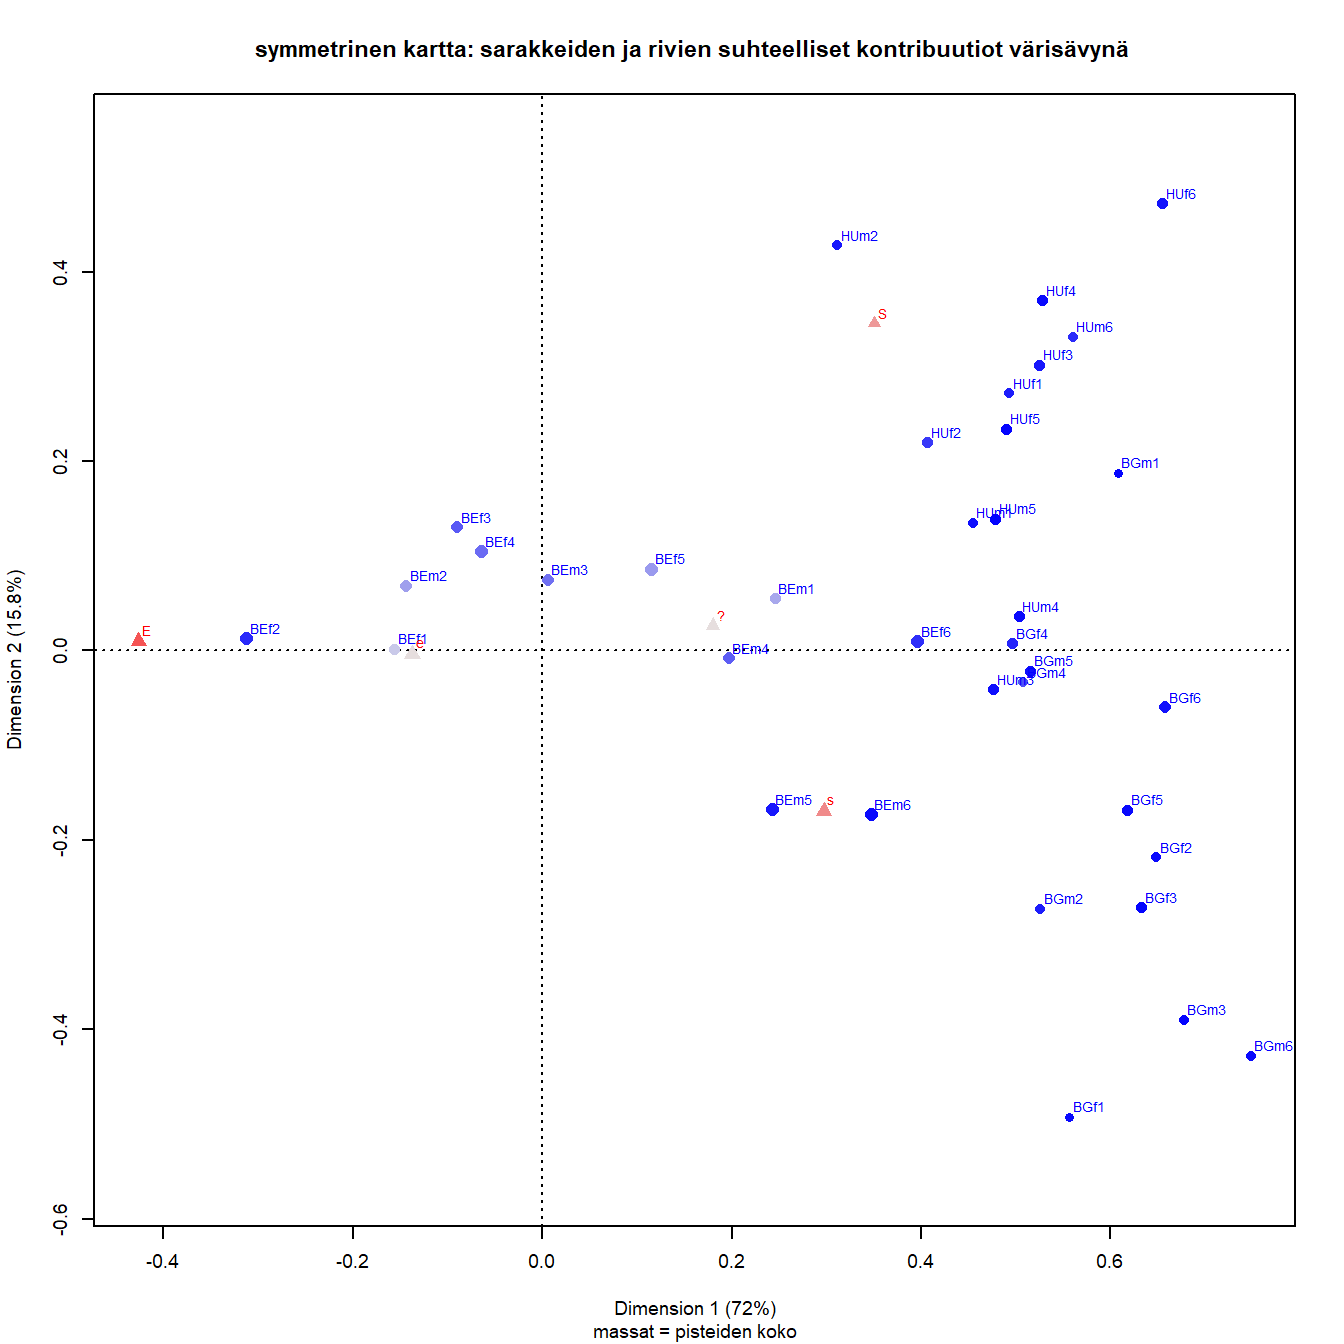
\includegraphics[width=0.9\linewidth]{JH_capaper_files/figure-latex/maagaCA2sub3map1-1} 

}

\caption{Ikä, sukupuoli ja maa: Belgia-Bulgaria - Unkari}\label{fig:maagaCA2sub3map1}
\end{figure}

\begin{Shaded}
\begin{Highlighting}[]
\CommentTok{# Vilkaistaa numeerisia tuloksia, kopioidaan tekstiin jos on tarpeen}
\CommentTok{# maagaCA2sub3}
 \KeywordTok{summary}\NormalTok{(maagaCA2sub3)}
\end{Highlighting}
\end{Shaded}

\begin{verbatim}
## 
## Principal inertias (eigenvalues):
## 
##  dim    value      %   cum%   scree plot               
##  1      0.086111  72.0  72.0  ******************       
##  2      0.018841  15.8  87.8  ****                     
##  3      0.011172   9.3  97.1  **                       
##  4      0.003477   2.9 100.0  *                        
##         -------- -----                                 
##  Total: 0.119602 100.0                                 
## 
## 
## Rows:
##      name   mass  qlt  inr    k=1 cor ctr    k=2 cor ctr  
## 1  | BEf1 |   14  152   19 | -156 152   4 |    2   0   0 |
## 2  | BEf2 |   24  826   24 | -313 824  28 |   13   1   0 |
## 3  | BEf3 |   21  623    7 |  -90 201   2 |  130 422  19 |
## 4  | BEf4 |   24  556    6 |  -65 155   1 |  105 401  14 |
## 5  | BEf5 |   23  355   11 |  115 227   3 |   86 128   9 |
## 6  | BEf6 |   23  810   37 |  396 810  41 |   10   0   0 |
## 7  | BEm1 |   11  288   21 |  246 274   8 |   55  14   2 |
## 8  | BEm2 |   17  333   11 | -144 271   4 |   68  61   4 |
## 9  | BEm3 |   20  531    2 |    6   4   0 |   75 528   6 |
## 10 | BEm4 |   22  620   11 |  197 618  10 |   -8   1   0 |
## 11 | BEm5 |   22  917   18 |  243 620  15 | -168 297  33 |
## 12 | BEm6 |   26  977   33 |  347 782  36 | -173 195  41 |
## 13 | BGf1 |    5  979   23 |  557 549  18 | -492 430  63 |
## 14 | BGf2 |    8  974   32 |  649 875  38 | -219  99  20 |
## 15 | BGf3 |   12 1000   46 |  633 844  54 | -271 155  45 |
## 16 | BGf4 |   10  847   25 |  496 847  30 |    7   0   0 |
## 17 | BGf5 |   14  961   50 |  618 894  62 | -168  66  21 |
## 18 | BGf6 |   18  939   71 |  658 931  92 |  -60   8   4 |
## 19 | BGm1 |    5  999   15 |  608 912  19 |  188  87   9 |
## 20 | BGm2 |    6  892   21 |  526 703  20 | -273 189  25 |
## 21 | BGm3 |    8  994   41 |  677 746  43 | -390 247  64 |
## 22 | BGm4 |    8  669   25 |  508 666  23 |  -34   3   0 |
## 23 | BGm5 |   10  949   24 |  516 947  32 |  -22   2   0 |
## 24 | BGm6 |    9  978   58 |  748 737  60 | -428 241  89 |
## 25 | HUf1 |    7  888   20 |  493 681  19 |  271 207  26 |
## 26 | HUf2 |   11  762   25 |  406 589  20 |  220 173  27 |
## 27 | HUf3 |   12  916   39 |  525 688  37 |  301 227  56 |
## 28 | HUf4 |   11  970   40 |  528 651  36 |  370 319  81 |
## 29 | HUf5 |   12  985   29 |  490 802  32 |  234 183  34 |
## 30 | HUf6 |   13  933   75 |  655 614  64 |  472 319 151 |
## 31 | HUm1 |    6  948   12 |  455 871  14 |  135  77   6 |
## 32 | HUm2 |    9  902   24 |  312 313  10 |  428 589  90 |
## 33 | HUm3 |   13  945   26 |  477 938  33 |  -41   7   1 |
## 34 | HUm4 |   10  965   22 |  503 960  29 |   36   5   1 |
## 35 | HUm5 |   13  993   26 |  478 916  33 |  139  77  13 |
## 36 | HUm6 |    8  839   33 |  560 622  29 |  331 217  46 |
## 
## Columns:
##     name   mass  qlt  inr    k=1 cor ctr    k=2 cor ctr  
## 1 |    S |   99  944  214 |  351 479 142 |  346 465 630 |
## 2 |    s |  238  942  247 |  297 711 244 | -169 231 362 |
## 3 |      |  168  435  107 |  180 426  63 |   26   9   6 |
## 4 |    e |  261  640   65 | -138 639  57 |   -4   0   0 |
## 5 |    E |  234  966  368 | -426 965 494 |   10   1   1 |
\end{verbatim}

\begin{Shaded}
\begin{Highlighting}[]
\CommentTok{# kahden osaratkaisun kokonaisinertia}

\CommentTok{# 0.143551 + 0.119602 = 0.263153}
\CommentTok{# koko datalla 0.263154}
\end{Highlighting}
\end{Shaded}

Kahden osajoukon inertioiden summa on sama kuin koko aineiston, Selitysasteet
kuitenkin nousevat, mutta vielä oleellisempaa on kahden aika erilaisen ryhmän
havaitseminen.

Belgian jotkun pisteet: huono kvaliteetti (BEf1, BEf5,BEm1, BEm2). Bulgaria ja
Unkari hyvin esitetty. Belgia on pulmallinen tapaus, omissa dimensioissaan.

\hypertarget{monimuuttuja-korrespondenssianalyysi-mca}{%
\chapter{Monimuuttuja-korrespondenssianalyysi (MCA)}\label{monimuuttuja-korrespondenssianalyysi-mca}}

\textbf{k} MG:n jäsentely CA:n tutkimusasetelmista (within - between), kokoaan myös
edeltävät analyysit ``saman katon alle''.

\textbf{k} Idea: taulukoiden yhdistely ``supertaulukoksi'' tai matriisiksi, analysoidaan kahden muuttujan
ristiintaulukoinnin laajennuksena useita kahden muuttujan ristiintaulukointeja.

\textbf{k} MCA stacked\&concat - analyysin erikoistapauksena.

\textbf{k} CA SVD:tä soveltavana ratkaisualgoritmina, jolle ``syötetään'' sopiva matriisi. Benzecri: löydettettävä vain
matriisi joka dekomponoidaan.

\textbf{k1} kahden muuttujuajoukon väliset yhteydet

\textbf{k2} yhden muuttujajoukon muuttujien väliset yhteydet

\textbf{k3} wrt samples ja wrt variables

\textbf{k4} Yksinkertaisesta monimutkaisempaan
0. Täydentävät pisteet tulkinnan apuna, yleistyökaluna (``jack of all trades but
master of none'') esitelty ensimmäisenä. Tärkeä lisä kaikissa analyyseissä.

\begin{enumerate}
\def\labelenumi{\arabic{enumi}.}
\item
  yhteisvaikutusmuuttujat \textbf{K4-1}
  -max kolmen muuttujan yhtesivaikutusmuuttuja - taulukko harsoontuu
\item
  Yksi ``selitettävä'' muuttuja, useampi ``selittävä'' \textbf{K4-2"}
\end{enumerate}

\begin{itemize}
\tightlist
\item
  pinotut taulukot (käytännössä matriisit, helpompi pinota R:ssä, Burtin taulun käyttö)
\end{itemize}

\begin{enumerate}
\def\labelenumi{\arabic{enumi}.}
\setcounter{enumi}{2}
\tightlist
\item
  Taulukoiden yhdistäminen yleisemmin \textbf{K4-3}
\end{enumerate}

\begin{itemize}
\tightlist
\item
  monta ``selittäjää'' ja ``selitettävää'': taulukoita päällekkäin ja rinnakkain, lohkomatriisi
\item
  ABBA: voidaan esim. jakaa taulukko (viite) osatauluiksi
\item
  tästä hieman tarkemmin teorialiitteessä;symmetriset taulut (esim. vastaukset
  eri vuosina, isän ja pojan ammatti), matched matrices
\end{itemize}

\begin{enumerate}
\def\labelenumi{\arabic{enumi}.}
\setcounter{enumi}{3}
\tightlist
\item
  MCA \textbf{K4-4}
\end{enumerate}

\textbf{K-n}

\textbf{tulkinnan tärkeimmät periaatteet}

\begin{itemize}
\tightlist
\item
  kaikki erot suhteellisia eroja
\item
  ca-ratkaisu approksimaatio; voi olla hyvä, mutta myös huono
  -CA on hajonnan (intertian) dekomponoinnin menetelmä.
\item
  Toiset (esim. MG,``ranskalaiset'') painottavat graafista menetelmää ja kuvien oikeaa tulkintaa),
  voi ymmärtää myös moniulotteisenä skaalauksena (MDS: etsi skaalaus, joka maksimoi
  korrelaation) tai moniulotteisena varianssianalyysinä (ANOVA)
\item
  tulkinnan tarkennus molemmissa alaluvuissa
\end{itemize}

**edit* Tässä jaksossa korostuu data-analyyin eksplotatiivinen luonne, datan kaivelu
ja näkökulmien muuntelu. Missä dimensiossa yhteydet ja riippuvuudet piileksivät?
Kartta on tässä mielessä kartta(vaikka hieman outo), osoittaa yhdessä numeeristen
tulosten kanssa suuntaa.

\hypertarget{pinotut-ja-yhdistetyt-taulukot-stacked-and-concatenated-tables}{%
\section{Pinotut ja yhdistetyt taulukot (stacked and concatenated tables)}\label{pinotut-ja-yhdistetyt-taulukot-stacked-and-concatenated-tables}}

Pinotut taulut: perusidea

\begin{Shaded}
\begin{Highlighting}[]
\NormalTok{knitr}\OperatorTok{::}\KeywordTok{include_graphics}\NormalTok{(}\StringTok{'img/stacked1.png'}\NormalTok{)}
\end{Highlighting}
\end{Shaded}

\begin{figure}

{\centering 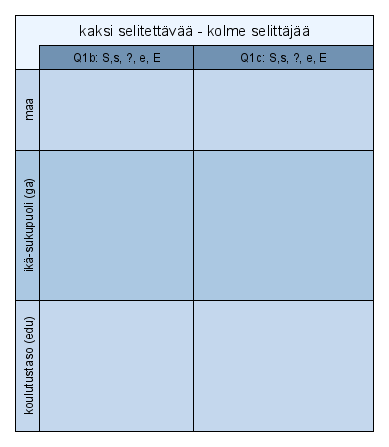
\includegraphics[width=0.5\linewidth]{img/stacked1} 

}

\caption{Pinotut ja yhdistetyt taulut - periaate}\label{fig:stackedimg1}
\end{figure}

Lisättiin kuva

Kun yhdistty taulu rakennetaan matriiseista, karttojen muuttujanimiä joudutaan
siistimään. Kuvat voivat myös herkästi kääntyä akselien ympäri, ne kannataa
kääntää vertailun helpottamiseksi samanlaisiksi kuin muut.

\begin{figure}

{\centering 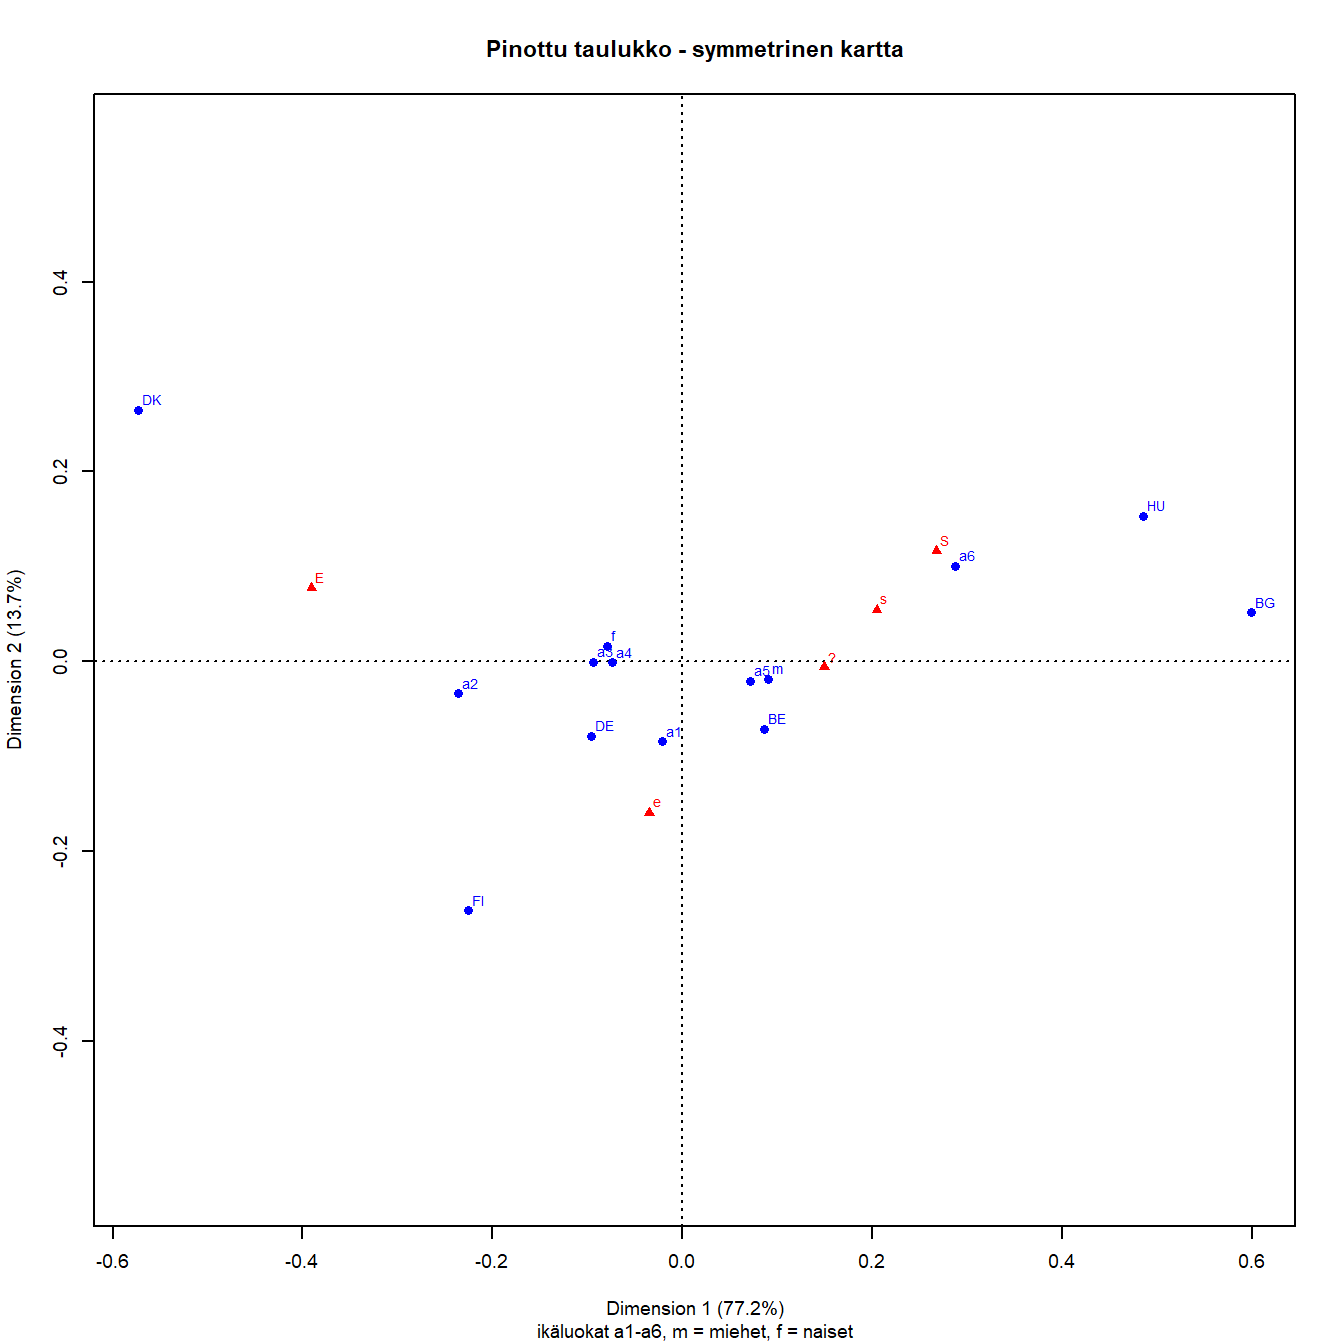
\includegraphics[width=0.9\linewidth]{JH_capaper_files/figure-latex/concat1map1-1} 

}

\caption{Q1b: Lapsi kärsii jos äiti käy työssä}\label{fig:concat1map1}
\end{figure}

\textbf{Kartan tulkinta; miten eroaa yhteisvaikutusmuuttujan analyysistä?}

Perustulkinta akseleille ei muutu, eikä maapisteiden sijoittuminenkaan.

Mikä on maapisteiden ja kahden selittävän (eksogeenisen) muuttujan pisteiden yhteys sarakepisteisiin?

Koko aineiston kartassa ikäluokkapisteet ja sukupuolipisteet ovat pakkautuneet maapisteitä tiiviimmin origon ympärille. Ikäluokkapisteiden (koko aineiston keskiarvot) selvä kontrasti on vanhimman (a6)ja toiseksi nuorimman välillä 1. dimenision suuntaan.

Ikäluokkapisteet ovat koko aineiston keskiarvopisteitä, niiden sijantia voi tulkita pistejoukko kerrallaan kuten maapisteidenkin. Mitään yhteisvaikutuksia ei analysoida eksplisiittisesti. Karttaa voi verrata sukupuoli-ikäluokka yhteisvaikutusmuuttujan analyysin aiemmin. Naispiste on tiukassa nipussa ikäluokkien a3 ja a4 kanssa aivan origon vasemmalla puolella. Miesten keskiarvopiste on hieman origosta oikealle, yhdessä ikäluokan a5 kanssa.

Taustamuuttujat: numeeristen tulosten tarkastelua

Lisäpisteet on hyvin esitetty, niiden etäisyyksiä voi luotettavasti arvioida kuvasta. Poikkeus on nuorin ikäluokka (a1, qlt = 501). Inertian osuudet (inr) ovat yhtä vaatimattomia kuin Belgian (28) ja Saksan (29), (m =20, f = 17, a2 = 40, a6 = 83), samoin kontribuutiot akseleiden inertiaan. 1. dimension kontribuutio (ctr) on suuri (\textgreater800) kaikilla paitsi nuorimmalla ikäryhmällä (a1) jolla 2. dimension selittää lähes puolet sen inertiasta (470).

Vilkaistaan taas numeerisa tuloksia, varmistetaan tulkinta. Tämän voi poistaa
lopullisesta versiosta.

\begin{Shaded}
\begin{Highlighting}[]
\KeywordTok{summary}\NormalTok{(Concat1jh.CA1)}
\end{Highlighting}
\end{Shaded}

\begin{verbatim}
## 
## Principal inertias (eigenvalues):
## 
##  dim    value      %   cum%   scree plot               
##  1      0.056877  77.2  77.2  *******************      
##  2      0.010116  13.7  91.0  ***                      
##  3      0.003923   5.3  96.3  *                        
##  4      0.002711   3.7 100.0  *                        
##         -------- -----                                 
##  Total: 0.073628 100.0                                 
## 
## 
## Rows:
##      name   mass  qlt  inr    k=1 cor ctr    k=2 cor ctr  
## 1  |   BE |   82  498   28 |   86 295  11 |  -71 203  41 |
## 2  |   BG |   38  907  204 |  599 901 238 |   52   7  10 |
## 3  |   DE |   70  498   29 |  -95 298  11 |  -78 200  43 |
## 4  |   DK |   57  990  310 | -573 816 328 |  265 175 394 |
## 5  |   FI |   45  987   75 | -225 419  40 | -262 568 309 |
## 6  |   HU |   41  856  168 |  486 778 169 |  153  78  95 |
## 7  |    m |  156  910   20 |   91 873  22 |  -19  37   5 |
## 8  |    f |  178  910   17 |  -79 873  20 |   16  37   5 |
## 9  |   a1 |   39  501    8 |  -22  31   0 |  -84 470  27 |
## 10 |   a2 |   50  958   40 | -236 939  49 |  -34  19   6 |
## 11 |   a3 |   56  958    7 |  -94 958   9 |   -1   0   0 |
## 12 |   a4 |   63  841    6 |  -74 841   6 |   -1   0   0 |
## 13 |   a5 |   62  868    5 |   71 801   6 |  -21  67   3 |
## 14 |   a6 |   63  957   83 |  288 852  92 |  101 104  63 |
## 
## Columns:
##     name   mass  qlt  inr    k=1 cor ctr    k=2 cor ctr  
## 1 |    S |   99  786  147 |  268 661 126 |  117 125 134 |
## 2 |    s |  238  843  172 |  205 787 175 |   55  56  70 |
## 3 |      |  168  640   80 |  150 639  66 |   -6   1   1 |
## 4 |    e |  261  970   97 |  -35  44   6 | -160 926 657 |
## 5 |    E |  234 1000  504 | -390 962 628 |   77  38 138 |
\end{verbatim}

\begin{Shaded}
\begin{Highlighting}[]
\CommentTok{# 14 riviä, inertiakontribuution keskiarvo}
\CommentTok{# 1000/14 = 71 }
\end{Highlighting}
\end{Shaded}

\textbf{edit} Galkussa myös subsetCA-kartta, josta Unkari ja Bulgaria on jätetty pois.
Ei mitään oleellista lisätietoa, joten ei esitetä tässä. Ensimmäisen dimension
osuus interitasta laskee ja toisen kasvaa. Kartan selkeys ei parane.

\begin{figure}

{\centering 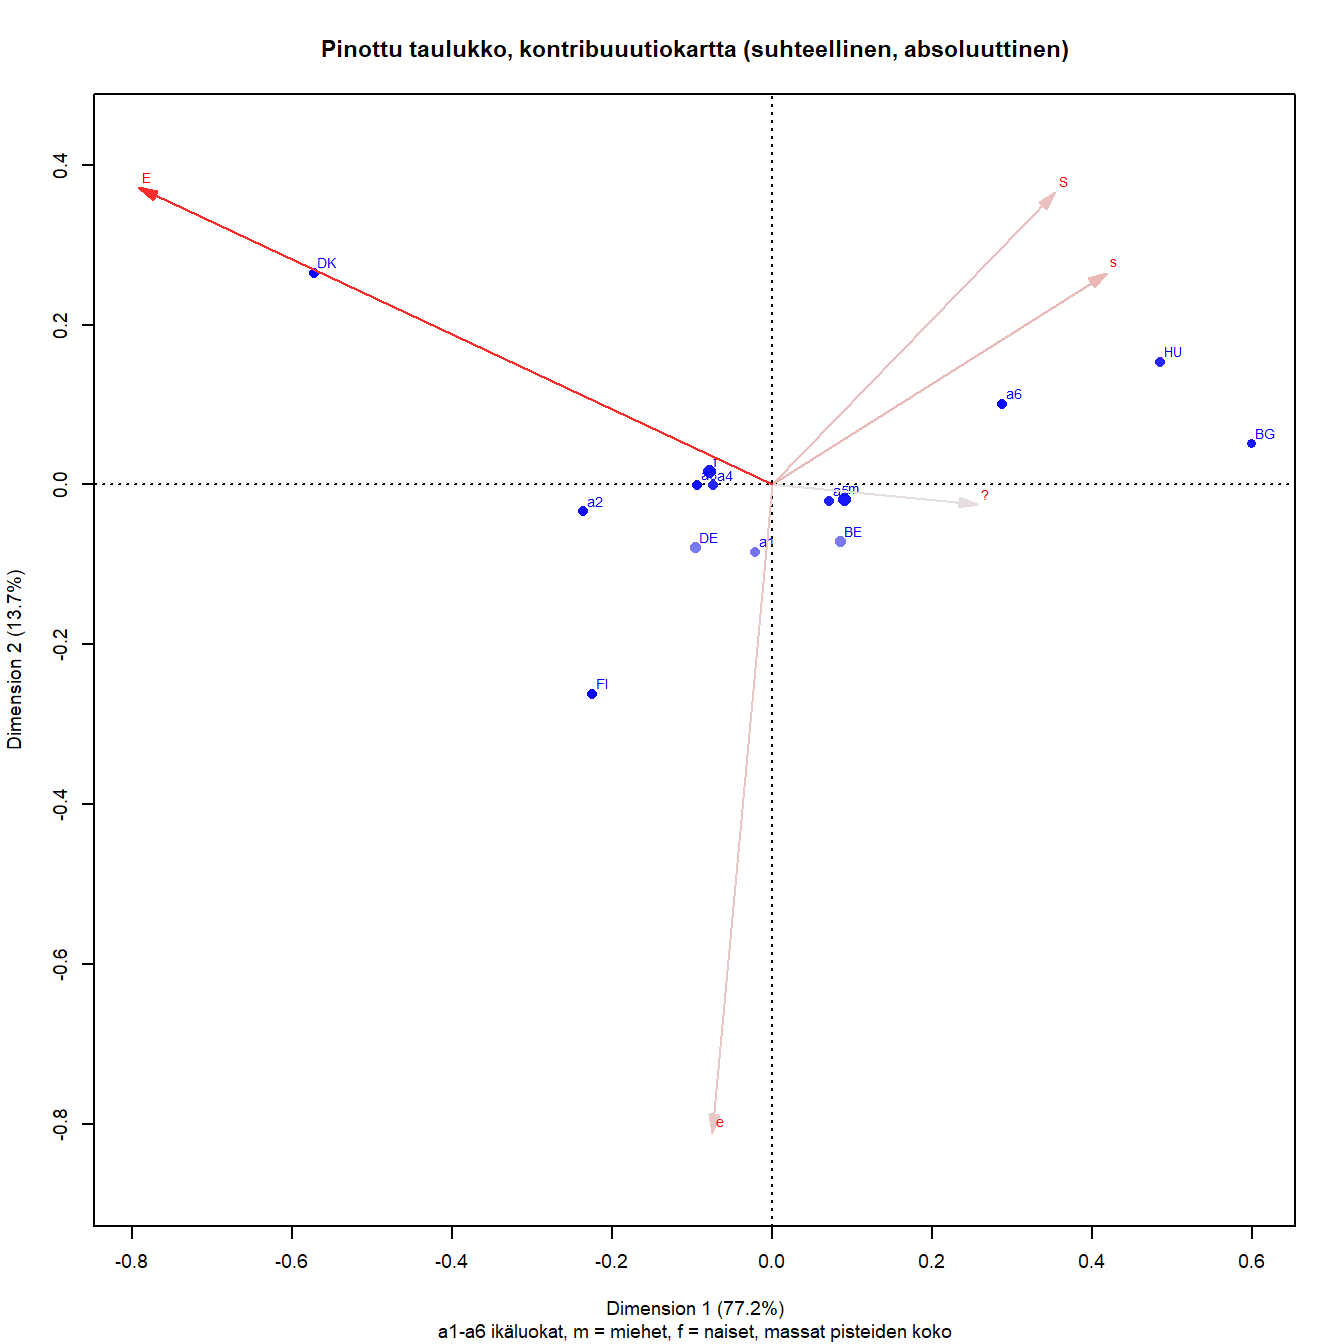
\includegraphics[width=0.9\linewidth]{JH_capaper_files/figure-latex/concat1map2-1} 

}

\caption{Q1b: Lapsi kärsii jos äiti käy työssä}\label{fig:concat1map2}
\end{figure}

Sarekkeista E-sarake (täysin eri mieltä) määrittää akseleita vahvasti, kontrastina
kaksi konservatiivista vastausta (S ja s) ja myös neutraali vaihtoehto (e).
Numeerista tuloksista nähdään, että ikäluokat vaikuttavat juuri ensimmäiseen tärkeimpään dimensioon.

Belgian ja Saksan pisteet on esitetty kartassa huonosti, samoin nuorin ikäluokka.
Muiden pisteiden sijaintia voidaan arvioida myös sarakkeiden ja rivipisteiden
välillä. Ikäluokkien kontrasti on selvä toiseksi nuorimman (a2) ja vanhimman (a6)
välillä.

\textbf{edit} Ikäluokkapisteet asymmetrisessä kontribuutiokartassa sarakkeiden keskiarvona,
samoin maapisteet. Esimerkiksi vanhimmassa ikäluokassa on suhteellisesti paljon
vastauksia samaa mieltä olevia ja neutraaleja ja vähän erimielisiä.

Hyvin yksinkertainen esimerkki.

\textbf{edit} Mutta tässä esimerkkiaineisto, jossa ei puuttuvia tietoja. Ne olisivatkin
aika pulmallisia, varianssin dekomponointi ei onnistu jos reunajakaumat ovat
alitauluissa erilaisia.

\hypertarget{matched-matrices}{%
\section{Matched matrices}\label{matched-matrices}}

\textbf{k} lyhyesti matriisien yhdistelystä hyvin yleisenä analyysin menetelmänä.
Voidaan tarkastella luonteeltaan erilaisten muuttujaryhmien tai muuttujien
yhteyksiä kuten edellisessä esimerkissä.

\textbf{Huom! (16.10.20} Jos ja kun ei tehdä analyysiä, ei tarvitse omaa jaksoa.
Kannattaa mainita, ehkävain teoriajaksossa? Idea: matriisien yhdistämisellä
saadaan ote monenlaiseen tutkimusongelmaan. Benzecri: data-analyysissä on vain
löydettävä oikea matriisi joka diagonalisoidaan.

Ref:CAip ss. 177 \citep{RefWorks:doc:5a857a43e4b0ed2d44664d78}, HY2017\_MCA, Greenacre JAS 2013
(sovellus ISSP 1989,4 kysymystä `pitäisikö äidin olla kotona', 8 maata), tässä
artikkelissa ``SVD-based methods'',joista yksi CA (muut biplots, PCA, compositional data/log ratios).
\citep{RefWorks:doc:5b6f159ce4b0bc0f31734b76}

\textbf{ABBA}``We consider the joint analysis of two matched matrices which have common
rows and columns, for example multivariate data observed at two time points or split
according to a dichotomous variable. Methods of interest include principal components
analysis for interval-scaled data, correspondence analysis for frequency data, log-ratio
analysis of compositional data and linear biplots in general, all of which depend on the
singular value decomposition. A simple result in matrix algebra shows that by setting up
two matched matrices in a particular block format, matrix sum and difference components
can be analysed using a single application of the singular value decomposition algorithm.
The methodology is applied to data from the International Social Survey Program
comparing male and female attitudes on working wives across eight countries. The resulting
biplots optimally display the overall cross-cultural differences as well as the male--female
differences. The case of more than two matched matrices is also discussed.''

Edellisen menetelmän variantti, jossa ryhmien väliset ja sisäiset erot saadaan
esiin. Inertian jakaminen.

Samanlaisten rivien ja sarakkeiden kaksi samankokoista taulua, esimerkiksi
sukupuolivaikutusten arviointi. Alkuperäinen taulukko jaetaan kahdeksi tauluksi
sukupuolen mukaan. Matriisien yhdistäminen (concatenation) riveittäin tai
sarakkeittain ei näytä optimaalisesti mm - matriisien eroja.

Ryhmien välisen ja ryhmien sisäinen inertian erottaminen, \textbf{ABBA}
on yksi ratkaisu (ABBA matrix, teknisesti block circular matrix).

Luokittelu voi olla myös kahden indikaattorimuuttujan avulla jako neljään
taulukkoon (esim. miehet vs.~naiset länsieuroopassa verratuna samaan asetelmaan
itä-Euroopassa). Samaa ideaa laajennetaan.

Esimerkkinä ``Attitudes to women working in 2012''.

\hypertarget{mca---monimuuttujakorrespondenssianalyysi}{%
\section{MCA - monimuuttujakorrespondenssianalyysi}\label{mca---monimuuttujakorrespondenssianalyysi}}

\textbf{k} Terminologiasta: monta muuttujaa on jo ollut käytössä. MCA on monimuuttujamenetelmä
samassa mielessä kuin faktorianalyysi. Analysoidaan usean statukseltaan samanlaisen
muuttujan välisiä suhteita, ja myös niiden yhteyksiä tutkimusongelman kannalta
``eksogeenisiin'' taustamuuttujiin tai ``selittäjiin''. Surveytutkimuksen kyselylomakkeen
kysymyspatterit luotaavat tietoa joistain taustalla olevista asenteista.

\textbf{edit} yksi kappale, jossa tutkimusasetelmaa verrataan tilastollisten mallien
asetelmaan? Jako ``selittäjiin'' ja selitettävään, moniyhtälömallit?
Faktorianalyysi tässä selkein vertailukohde

\textbf{k} Matemaattisesti kaikki muuttuu paljon mutkikkaammaksi, ja yksinkertaisen
perustapauksen selkeät tulkinnat eivät toimi. Tärkeä asia: CA:n skaalausominaisuudet ja
visuaalinen tulkinta pätevät edelleen.

\textbf{edit} Teorialiitteessä tästä enemmän, ranskalaiset hieman eri mieltä
\textbf{Viitteitä}

MG ja MG\&Prado ovat tutkineet ISSP-datalla tätä ongelmaa.
Biplots In practice - kirja \citep{RefWorks:doc:5a857a43e4b0ed2d44664d7c}, ss.142-
``dimensions of middleness''. Mg ja Prado artikkelissaan
\citep{RefWorks:doc:5a857a44e4b0ed2d44664d87} ja samasta teemasta laajentaen
kokoomateoksessa \citep{RefWorks:doc:5ab76b43e4b003f4468d1f07}, ss. 197-217.
Aineistona jälkimmäisessä tutkimuksessa on sama kysymyssarja kuin tässä 1994
datasta. Kysymyksissä on jonkin verran eroja. Ensimmäisessä artikkelissa he kommentoivat vertaisarvioitsijoiden ehdotuksia. Kuvia voisi selkiyttää esittämällä vain osan
pisteistä sarjassa karttoja, mutta ratkaisu perustuisi siinäkin koko dataan ja
sitä nimenomaan ei haluta. Toinen ehdotus on yhdistää ne vastausvaihtoehdot jotka
eivät ole tutkimuksen kohteena yhdeksi yhdistetyksi kategoriaksi. Tällöin osajoukon
korrespondenssianalyysin kätevä inertia dekomponointi osajoukille ei toimisi. Ratkaisu
ei toimi ollenkaan yleisimmissä osajoukoissa.

\textbf{k} Data

\textbf{k} Taustamuuttujien taulukoissa on yllättävän isoja eroja, jotkut taulukoiden luokat
ovat nollia tai hyvin vähän havaintoja. Luokkia pitäisi yhdistellä,jo pelkästään
``kuvaroskan'' takia. Ei tehdä.

\textbf{k} Puuttuvat havainnot, muutama numero vain mitä ``listwise delete'' saa aikaan.

\begin{Shaded}
\begin{Highlighting}[]
\CommentTok{#Puuttuvien tietojen yleiskuva}

\CommentTok{# Puuttuvat tiedot aineistossa - viite datan dokumentointiin jossa taulukot.}
\CommentTok{# Vaihtelee maittain ja muuttujittain, paljon.}

\CommentTok{# Koko data (G1_1_data2.Rmd - skriptissä valitut muuttujat ja 25 maata)}
\CommentTok{#}
\CommentTok{#sum(!complete.cases(ISSP2012jh1d.dat)) = 9455}
\CommentTok{#dim(ISSP2012jh1d.dat) = 32823}
\CommentTok{#9455/32823 = 0.2880602}

\CommentTok{# Puuttuvat tiedot valitussa MCA-aineistossa}

\CommentTok{#missingMCAvars1 <-  c("Q1a","Q1b", "Q1c", "Q1d","Q1e","Q2a","Q2b","edu",}
\CommentTok{#                 "sosta", "urbru", "maa", "ika", "sp" )}
\CommentTok{#missingTestMCA1.dat <- ISSP2012jh1d.dat %>% select(all_of(missingMCAvars1))}

\CommentTok{#sum(!complete.cases(missingTestMCA1.dat)) = 6101}
\CommentTok{#dim(missingTestMCA1.dat) = 32823}
\CommentTok{#6101/32823 = 0.1858758 Puuttellisten havaintojen osuus.}
\end{Highlighting}
\end{Shaded}

Koko tähän tutkimukseen valitussa aineistossa (25 maata ja muuttujat, poistettu
havainnot joissa ikä tai sukupuoli puuttuu) 71\% havainnoista on kaikki tiedot.

MCA-analyyseihin valitun 7 + 3 = 10 muuttujan aineiston havainnoista 81\% on
vailla puuttuvia tietoja. Jos puuttuvat tiedot poistetaan (ns. ``listwise delete'',
poistetaan jos yksi tai useampi tieto puuttuu) viidesosa datasta jää pois.

\textbf{k} lyhyt kappale - puuttuvien tietojen käsittely on laaja aihe. Otantamenetelmissä ja survey-aineistojen (kyselytutkimusten) oppaissa käsitelty monipuolisesti.

\textbf{k} Miten liittyy tähän? CA on koko aineiston kuvailevaa analyysiä, ei päättelyä
otoksesta perusjoukon tasolle. Miten puuttuvia vastauksia voisi kuvailla? Toisaalta
edellisen jakson menetelmien soveltaminen on mahdotonta, jos jotain ei tehdä
(reunajakaumat oltava samoja).

MCA1 - seitsemän kysymystä (jokaisessa viisi vaihtoehtoa)

Aineistossa on 32 823 havaintoa ja seitsemän muuttujaa.

\begin{figure}

{\centering 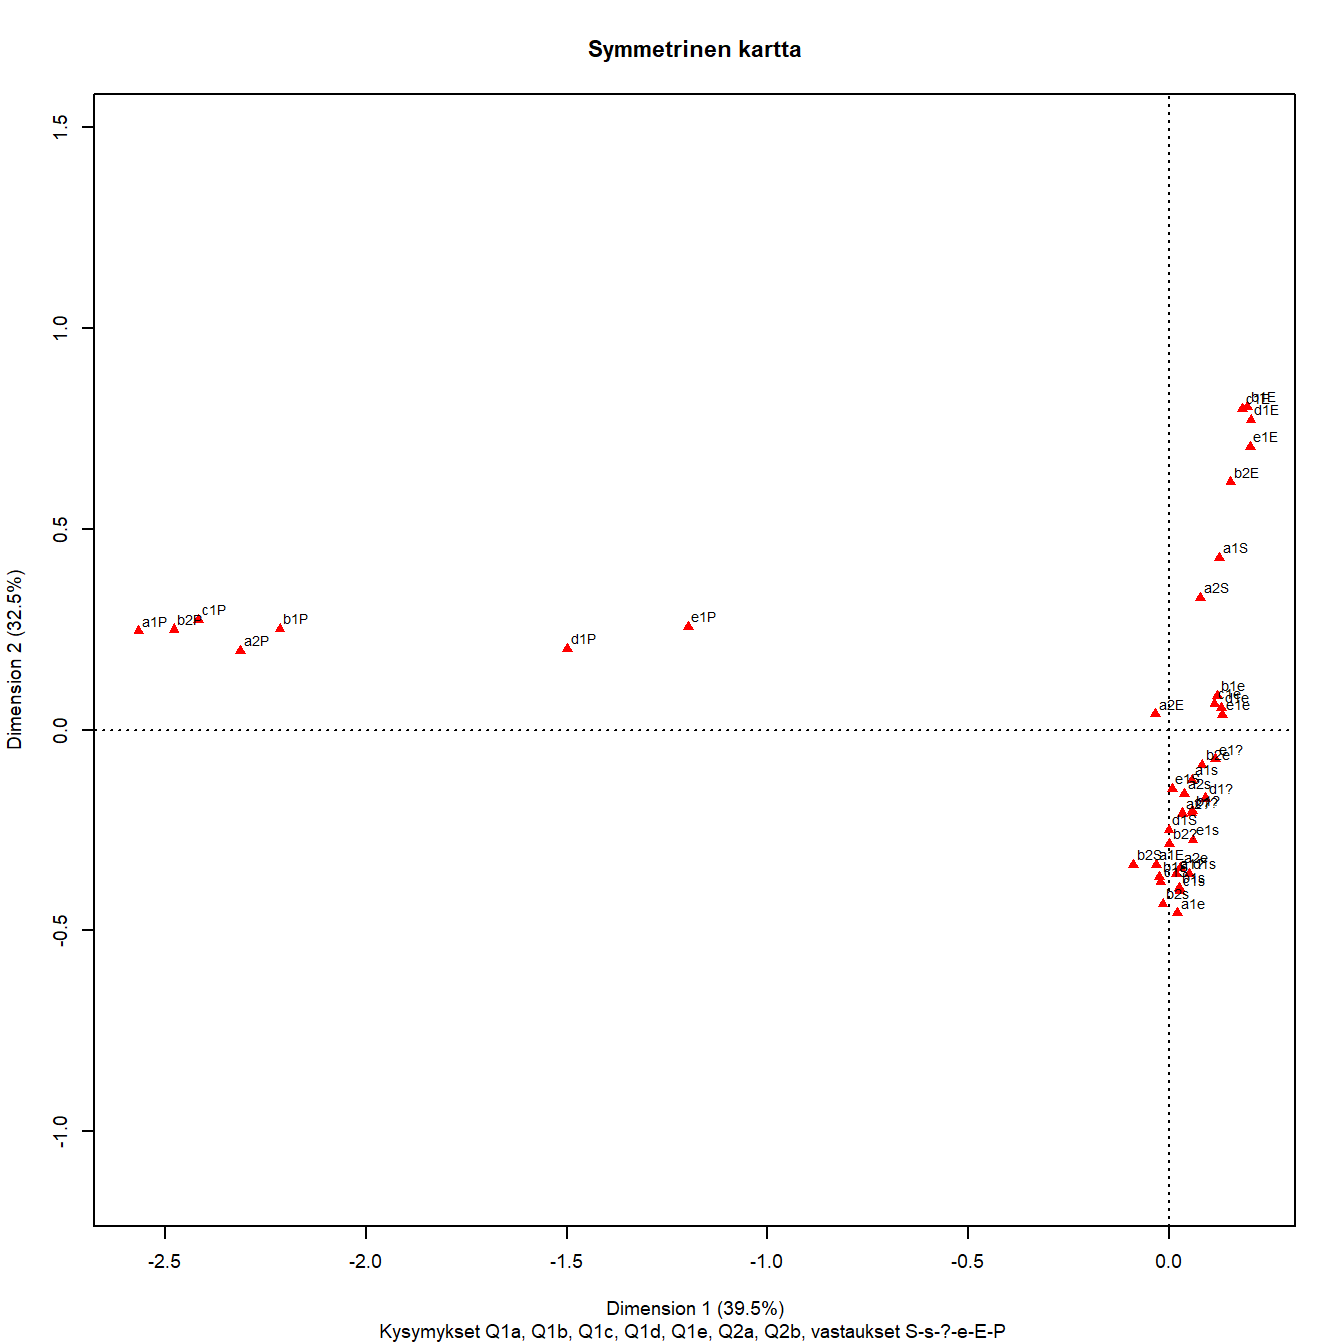
\includegraphics[width=0.9\linewidth]{JH_capaper_files/figure-latex/MCA1map1-1} 

}

\caption{MCA: Seitsemän kysymystä - 25 maata, kartta 1}\label{fig:MCA1map1}
\end{figure}

\textbf{k} Perustulkinta: Inertian selitysosuudet ovat paljon pienempiä, ja ratkaisu
on selvästi kaksiulotteinen. Puuttuvat vastaukset erottuvat omana ryhmänä, ja
varsinaiset vastaukset ovat pakkautuneet y-akselin oikealle puolelle. Niiden erot
näkyvät vain toisessa dimensiossa. Ensimmäinen dimensio kuvaa vastaamattomuutta (syystä tai toisesta) vs.~kaikkia vastauksia.

Pystyakselin suuntaan kontrasti näyttäisi olevan konservatiiviset ylhäällä,
modernit ja liberaalimmat alhaalla. Pisteitä on vaikea erottaa toisistaan.

Karttaa voi parantaa lisäämällä siihen vastaajien (n= 32 823) pisteet (viite MG - ekologiakirja, jossa vanhempi ISSP-data).

\begin{figure}

{\centering 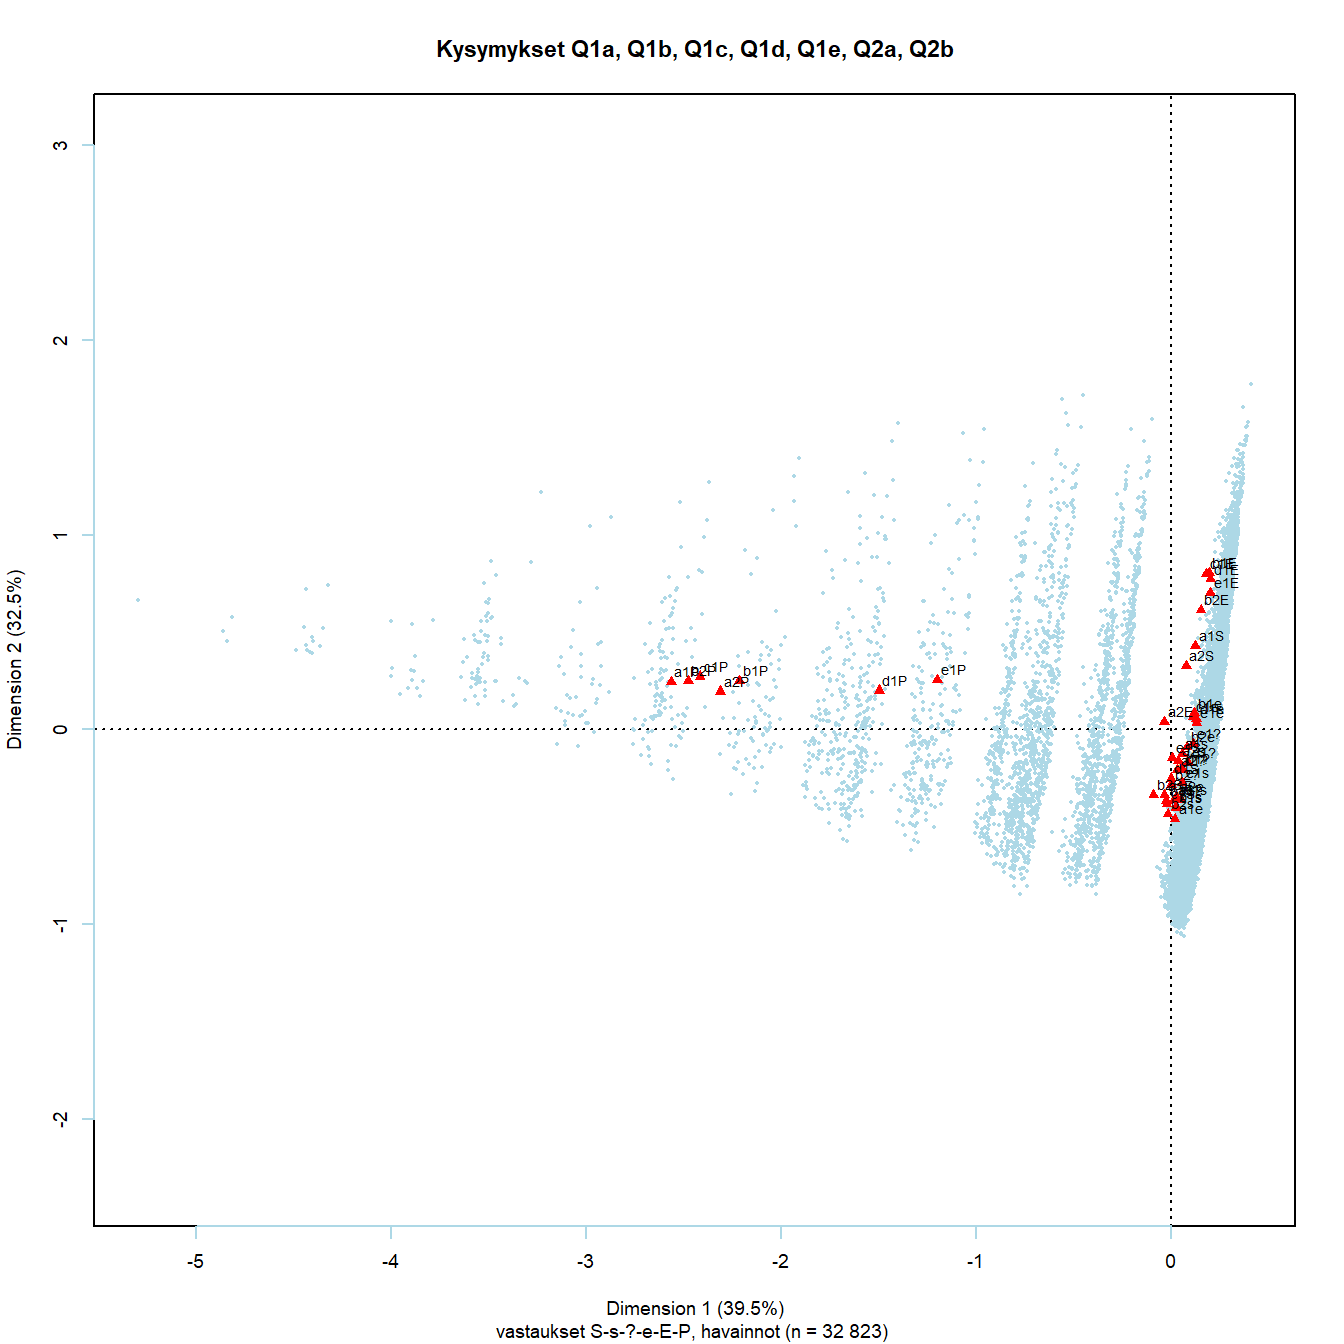
\includegraphics[width=0.9\linewidth]{JH_capaper_files/figure-latex/MCA1map2-1} 

}

\caption{MCA: Seitsemän kysymystä - 25 maata, kartta 2}\label{fig:MCA1map2}
\end{figure}

Jokainen havainto on sarakevektoreiden keskiarvopiste. Sarakevektoreita ei voi
tulkita yhtä selkeästi kuin yksinkertaisessa korrespondenssianalyysissä. Ne eivät
edusta kysymystä vaan kysymyksen yhtä vastauskategoriaa, pitkä jono nollia ja ykkösiä.
Rivipiste on vastauksiaan vastaavien sarakepisteiden keskiarvopiste. Jos vastaaja on valinnut
vaihtoehdot (a1S, a2s,\ldots, b2?) se on näiden pisteiden keskiarvopiste.

Oleellista MCA-kartan tulkinnassa on kuitenkin yleiskuvan muodostaminen, geometrinen
tulkinta on hieman hankala. Skaalausominaisuudet MCA kuitenkin säilyttää (\textbf{Viite},
teorialiitteessä hieman tarkemmin).

Myös riviprofiilit ovat samanlaisia, jokaisella rivilla on kuudessa kategoriassa (vastaukset
ja puuttuva tieto) nollia ja yksi ykkönen. Rivien välistä etäisyyttä määrittelevä ainoastaa
``erimielisyydet'', ja GDA-kirjan (\textbf{viite}) ohjeen mukaan MCA-karttojen tulkinta pitäisi aloittaa
yksilöiden pilven ääripäistä.

Pistepilven muoto kertoo , kuinka pienenevä joukko vastaajia lähestyy kiilana
puuttivien tietojen pisteitä. Kaikkiin kysymyksiin vastanneet ovat massana kuvan oikeassa laidassa. Pistepilvet
oikealta vasemmalle kuvaavat kuinka moneen kysymykseen on jätetty vastaamatta.

(MG-vastaava kuva \citep{RefWorks:doc:5a857a43e4b0ed2d44664d7c}, luku 14. ``dimenisions of middleness''.)
Pieni joukko määrää koko kartan koordinaatiston.

\textbf{Osajoukon MCA}

\textbf{k} Osajoukon MCA ratkaisee ongelman tyylikkäästi.

\begin{figure}

{\centering 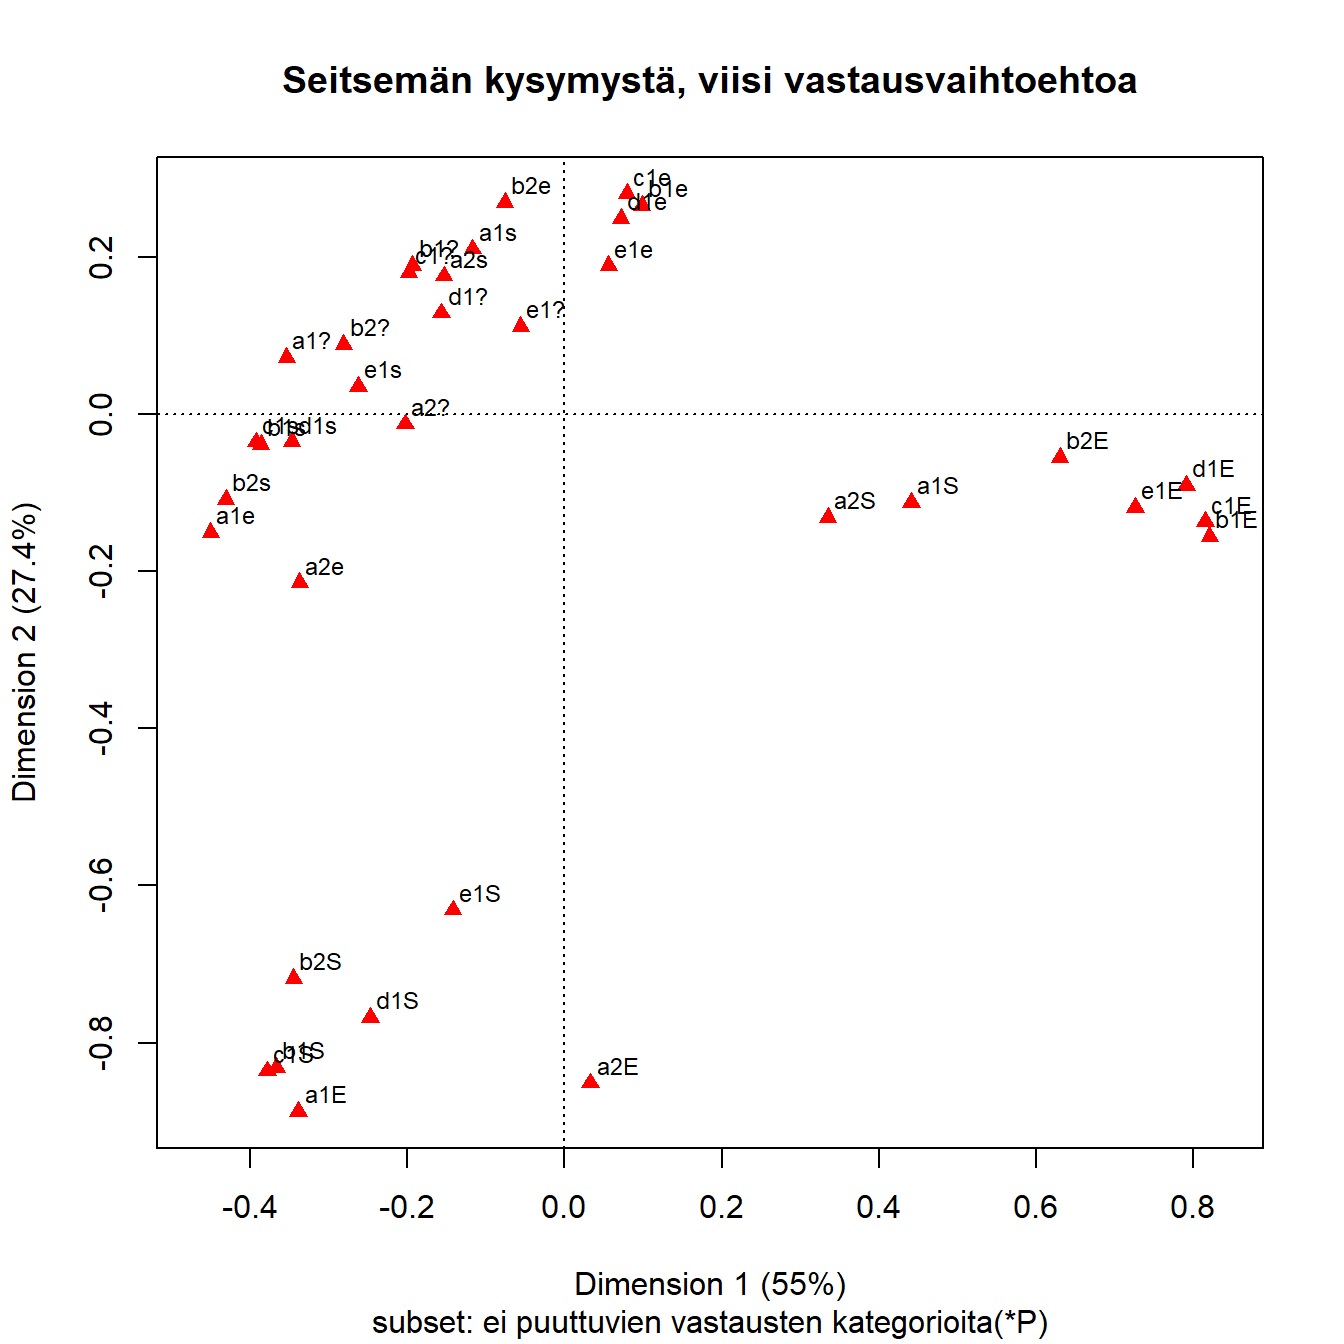
\includegraphics[width=0.9\linewidth]{JH_capaper_files/figure-latex/subsetMCA1map1-1} 

}

\caption{MCA: Seitsemän kysymystä - 25 maata, kartta 3}\label{fig:subsetMCA1map1}
\end{figure}

\textbf{k} Tulkinta: kontrasti ``ääripäiden'' välillä, vahvat mielipiteet (S ja E) hallitsevat vasenta alakulmaa ja oikeaa laitaa x-akselin tuntumassa. Maltilliset
vastaukset ja neutraali vaihtoehto ovat ylhäällä vasemmalla.

\textbf{k} Johtopäätös: seitsemän kysymystä erottelee hyvin vastaajat
liberaali - konservatiivi - aksellilla. Maltilliset ja neutraalit vastaukset sijaitsevat ääripäiden välissä. Karttaan voi hahmotella diagonaalin suuntaisen
akselin vahvojen mielipiteiden ryppäiden välille. Muut vastaukset ovat
ns. kaariefektin mukaisesti näiden välisellä U-muotoisella linjalla. Tämä kuuluisa Guttan efekti kertoo järjestysasteikon muuttujien korrelaatiosta, hyvä asia kun
kysymyksillä luodataan asenteita naisten työssäkäyntiin. Kaariefekti on myös ``geometrinen välttämättömyys'', tarkemmin teorialiitteessä.

\begin{figure}

{\centering 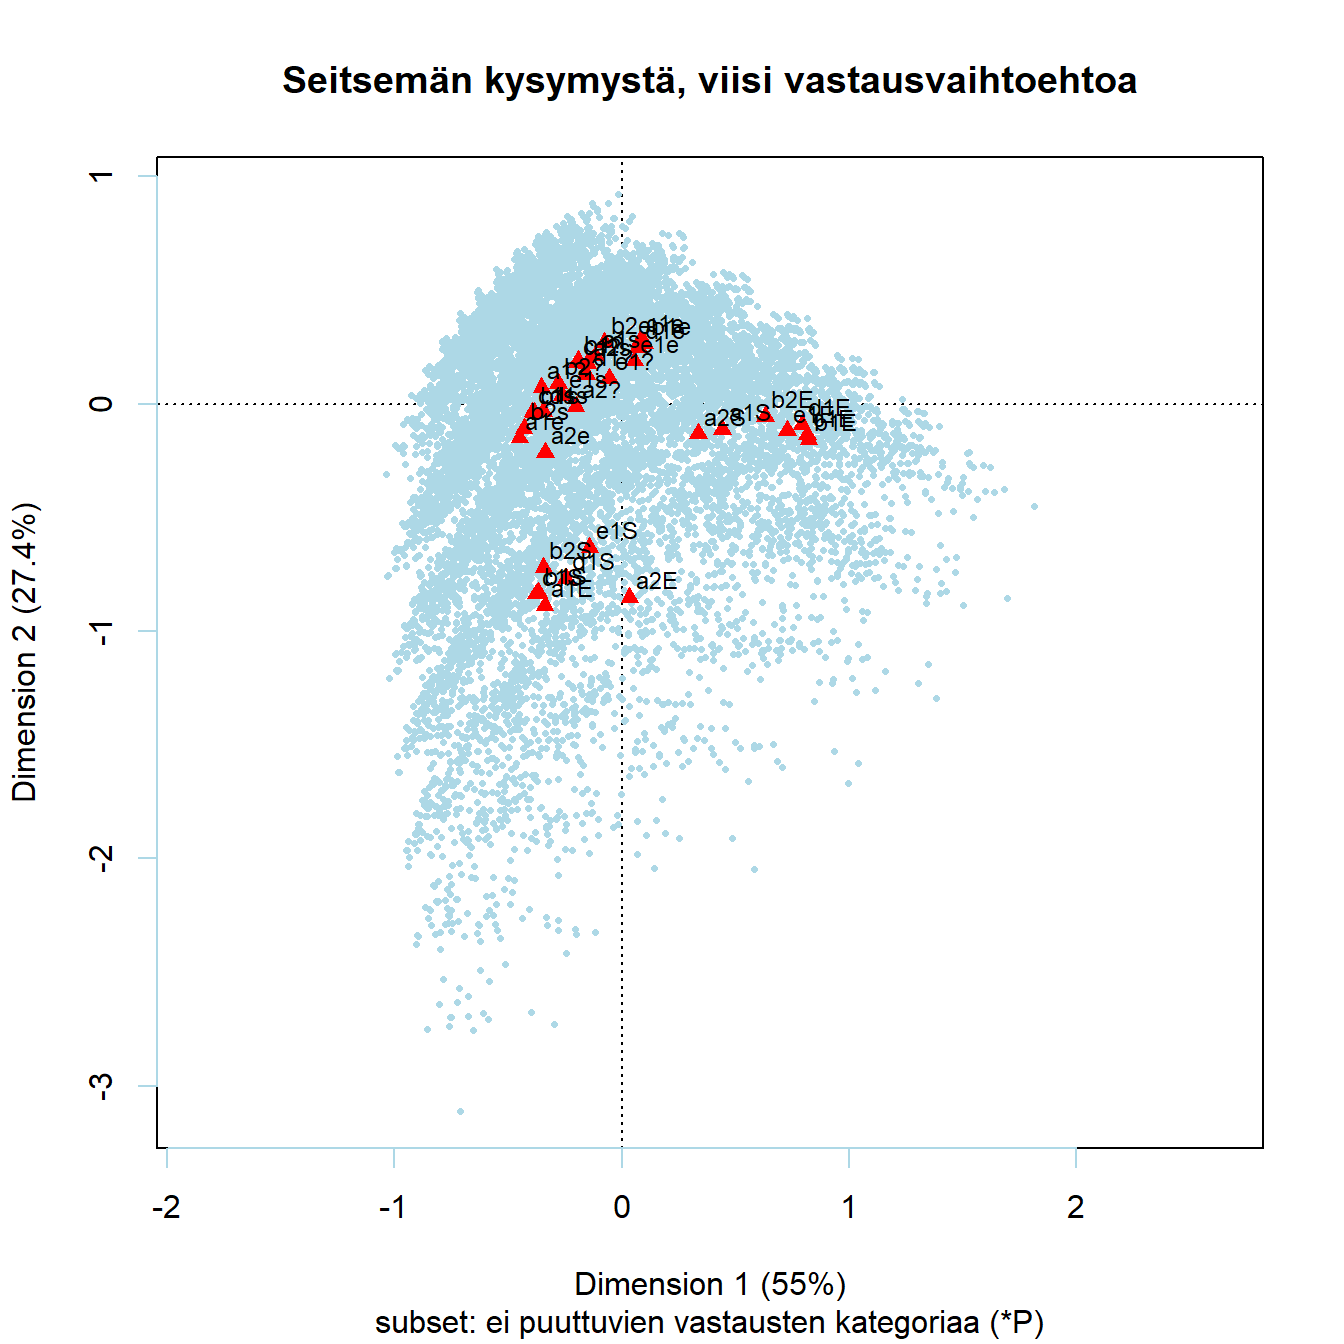
\includegraphics[width=0.9\linewidth]{JH_capaper_files/figure-latex/subsetMCA1map2-1} 

}

\caption{MCA: Seitsemän kysymystä - 25 maata, kartta 4}\label{fig:subsetMCA1map2}
\end{figure}

Kun kartalle lisätään havainnot, nähdään selvästi kuinka suuri hajonta on havaintojen
pilvessä verrattuna vastauskategorioiden pilveen.

Asymmetrinen kartta näyttäisi olevan paras vaihtoehto, vastausvaihtoehdot erottuvat selvemmin.

\begin{figure}

{\centering 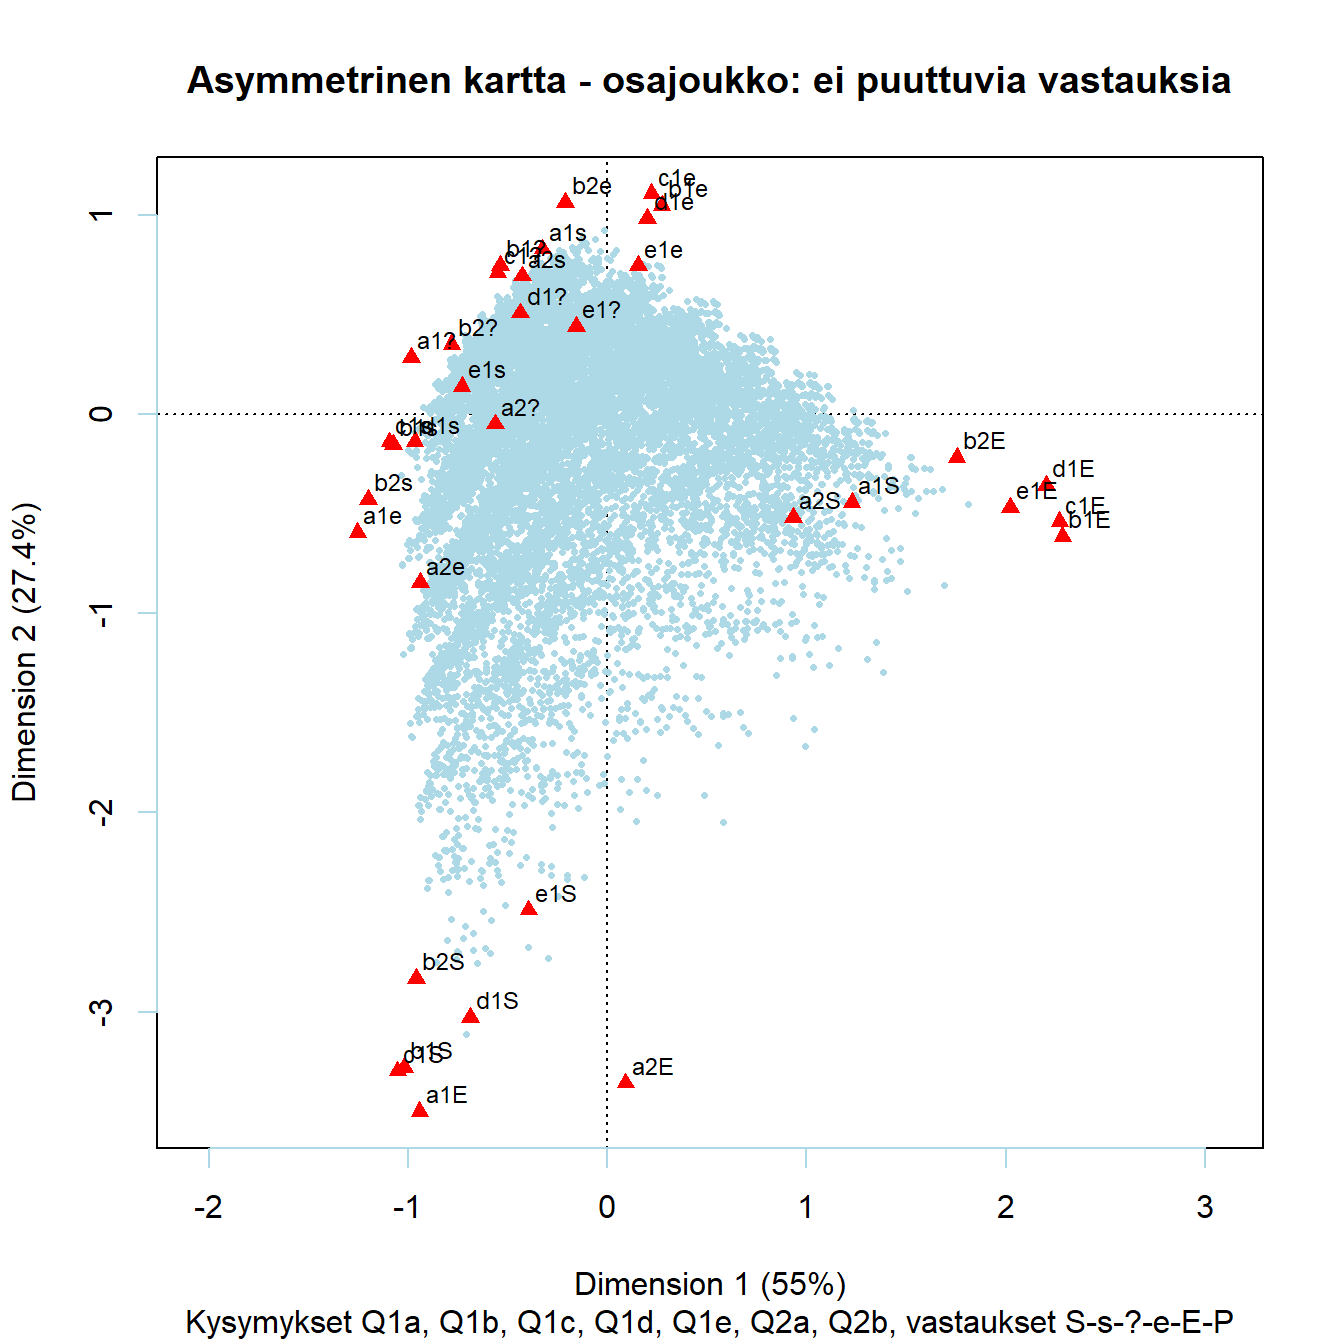
\includegraphics[width=0.9\linewidth]{JH_capaper_files/figure-latex/subsetMCA1map3-1} 

}

\caption{MCA: Seitsemän kysymystä - 25 maata, kartta 5}\label{fig:subsetMCA1map3}
\end{figure}

\textbf{edit1} Jostain syystä en saa toimimaan mjca-funktiossa subsecat - parametrin kanssa
täydentäviä muuttujia supcol.

\textbf{edit2}
\textbf{MCA - numeeriset tulokset}

\begin{Shaded}
\begin{Highlighting}[]
\KeywordTok{summary}\NormalTok{(Qmuuttujat2.mca)}
\end{Highlighting}
\end{Shaded}

\begin{verbatim}
## 
## Principal inertias (eigenvalues):
## 
##  dim    value      %   cum%   scree plot               
##  1      0.129087  55.0  55.0  ***************          
##  2      0.064296  27.4  82.4  *******                  
##  3      0.014807   6.3  88.7  **                       
##  4      0.008871   3.8  92.5  *                        
##  5      0.000538   0.2  92.7                           
##  6      0.000221   0.1  92.8                           
##  7      0.000156   0.1  92.9                           
##  8      6.9e-050   0.0  92.9                           
##  9      1e-06000   0.0  92.9                           
##         -------- -----                                 
##  Total: 0.234728                                       
## 
## 
## Columns:
##      name   mass  qlt  inr    k=1 cor ctr    k=2 cor ctr  
## 1  |  a1S |   48  975   29 |  441 916  73 | -112  59   9 |
## 2  |  a1s |   54  869   20 | -117 206   6 |  210 663  37 |
## 3  |  a1? |   15  653   27 | -354 626  14 |   73  26   1 |
## 4  |  a1e |   18  788   29 | -451 709  28 | -150  79   6 |
## 5  |  a1E |    5  884   30 | -339 113   4 | -887 771  56 |
## 6  |  b1S |   12  818   37 | -367 133  12 | -831 685 128 |
## 7  |  b1s |   37  696   28 | -387 689  42 |  -39   7   1 |
## 8  |  b1? |   26  527   25 | -194 269   8 |  189 258  14 |
## 9  |  b1e |   39  555   25 |   98  67   3 |  266 488  43 |
## 10 |  b1E |   24  889   43 |  821 858 126 | -156  31   9 |
## 11 |  c1S |   12  826   38 | -379 141  14 | -836 685 134 |
## 12 |  c1s |   36  698   29 | -393 692  43 |  -35   6   1 |
## 13 |  c1? |   26  517   25 | -198 282   8 |  181 235  13 |
## 14 |  c1e |   38  550   26 |   79  41   2 |  281 509  46 |
## 15 |  c1E |   26  890   43 |  815 865 134 | -137  24   8 |
## 16 |  d1S |   12  851   34 | -247  80   6 | -768 771 112 |
## 17 |  d1s |   33  751   26 | -347 744  31 |  -35   8   1 |
## 18 |  d1? |   32  561   23 | -157 336   6 |  129 226   8 |
## 19 |  d1e |   34  620   24 |   72  47   1 |  249 572  33 |
## 20 |  d1E |   22  944   38 |  791 932 106 |  -91  12   3 |
## 21 |  e1S |   15  910   31 | -142  44   2 | -631 866  90 |
## 22 |  e1s |   36  752   23 | -263 738  19 |   35  13   1 |
## 23 |  e1? |   34  350   22 |  -56  70   1 |  112 279   7 |
## 24 |  e1e |   32  597   23 |   56  48   1 |  189 549  18 |
## 25 |  e1E |   15 1012   32 |  726 985  62 | -119  26   3 |
## 26 |  a2S |   49 1005   24 |  335 870  43 | -132 134  13 |
## 27 |  a2s |   59  989   19 | -154 428  11 |  176 561  28 |
## 28 |  a2? |   22  584   24 | -203 582   7 |  -12   2   0 |
## 29 |  a2e |    8  794   26 | -338 565   7 | -215 228   6 |
## 30 |  a2E |    2  870   27 |   33   1   0 | -851 869  20 |
## 31 |  b2S |   12  922   33 | -345 173  11 | -718 750  94 |
## 32 |  b2s |   22  783   28 | -431 736  32 | -108  46   4 |
## 33 |  b2? |   27  640   25 | -281 582  16 |   89  58   3 |
## 34 |  b2e |   40  711   24 |  -76  53   2 |  269 658  45 |
## 35 |  b2E |   39  939   37 |  630 932 119 |  -55   7   2 |
\end{verbatim}

Vilkaistaan 3d-ratkaisua - onko kolmella keskimmäisellä vaihtoehdolla ``dimenison
of middleness''?

\textbf{edit} tämä poistetaan lopullisesta versiosta.

\begin{Shaded}
\begin{Highlighting}[]
\NormalTok{Qmuuttujat2d3  <-}\StringTok{ }\KeywordTok{mjca}\NormalTok{(mcaDat11jh.dat, }\DataTypeTok{ps=}\StringTok{""}\NormalTok{, }\DataTypeTok{nd =} \DecValTok{3}\NormalTok{,}\DataTypeTok{subsetcat=}\NormalTok{eiPvastaukset)}
\KeywordTok{summary}\NormalTok{(Qmuuttujat2d3)}
\end{Highlighting}
\end{Shaded}

\begin{verbatim}
## 
## Principal inertias (eigenvalues):
## 
##  dim    value      %   cum%   scree plot               
##  1      0.129087  55.0  55.0  ***************          
##  2      0.064296  27.4  82.4  *******                  
##  3      0.014807   6.3  88.7  **                       
##  4      0.008871   3.8  92.5  *                        
##  5      0.000538   0.2  92.7                           
##  6      0.000221   0.1  92.8                           
##  7      0.000156   0.1  92.9                           
##  8      6.9e-050   0.0  92.9                           
##  9      1e-06000   0.0  92.9                           
##         -------- -----                                 
##  Total: 0.234728                                       
## 
## 
## Columns:
##      name   mass  qlt  inr    k=1 cor ctr    k=2 cor ctr    k=3 cor ctr  
## 1  |  a1S |   48  976   29 |  441 916  73 | -112  59   9 |  -18   1   1 |
## 2  |  a1s |   54  966   20 | -117 206   6 |  210 663  37 |   81  98  24 |
## 3  |  a1? |   15  786   27 | -354 626  14 |   73  26   1 | -163 133  26 |
## 4  |  a1e |   18  837   29 | -451 709  28 | -150  79   6 | -119  49  17 |
## 5  |  a1E |    5  935   30 | -339 113   4 | -887 771  56 |  229  51  16 |
## 6  |  b1S |   12  869   37 | -367 133  12 | -831 685 128 |  226  51  41 |
## 7  |  b1s |   37  798   28 | -387 689  42 |  -39   7   1 | -149 102  55 |
## 8  |  b1? |   26  573   25 | -194 269   8 |  189 258  14 |  -80  46  11 |
## 9  |  b1e |   39  836   25 |   98  67   3 |  266 488  43 |  201 281 107 |
## 10 |  b1E |   24  910   43 |  821 858 126 | -156  31   9 | -129  21  27 |
## 11 |  c1S |   12  876   38 | -379 141  14 | -836 685 134 |  226  50  43 |
## 12 |  c1s |   36  805   29 | -393 692  43 |  -35   6   1 | -155 107  58 |
## 13 |  c1? |   26  571   25 | -198 282   8 |  181 235  13 |  -87  54  13 |
## 14 |  c1e |   38  843   26 |   79  41   2 |  281 509  46 |  213 293 116 |
## 15 |  c1E |   26  908   43 |  815 865 134 | -137  24   8 | -119  18  25 |
## 16 |  d1S |   12  902   34 | -247  80   6 | -768 771 112 |  197  51  32 |
## 17 |  d1s |   33  828   26 | -347 744  31 |  -35   8   1 | -112  77  28 |
## 18 |  d1? |   32  647   23 | -157 336   6 |  129 226   8 |  -80  86  14 |
## 19 |  d1e |   34  896   24 |   72  47   1 |  249 572  33 |  173 276  69 |
## 20 |  d1E |   22  956   38 |  791 932 106 |  -91  12   3 |  -90  12  12 |
## 21 |  e1S |   15  949   31 | -142  44   2 | -631 866  90 |  135  40  18 |
## 22 |  e1s |   36  793   23 | -263 738  19 |   35  13   1 |  -62  42  10 |
## 23 |  e1? |   34  475   22 |  -56  70   1 |  112 279   7 |  -75 126  13 |
## 24 |  e1e |   32  847   23 |   56  48   1 |  189 549  18 |  128 250  35 |
## 25 |  e1E |   15 1023   32 |  726 985  62 | -119  26   3 |  -78  11   6 |
## 26 |  a2S |   49 1005   24 |  335 870  43 | -132 134  13 |   -2   0   0 |
## 27 |  a2s |   59 1011   19 | -154 428  11 |  176 561  28 |   35  22   5 |
## 28 |  a2? |   22  770   24 | -203 582   7 |  -12   2   0 | -115 186  19 |
## 29 |  a2e |    8  796   26 | -338 565   7 | -215 228   6 |   23   3   0 |
## 30 |  a2E |    2  920   27 |   33   1   0 | -851 869  20 |  202  49   5 |
## 31 |  b2S |   12  961   33 | -345 173  11 | -718 750  94 |  162  38  21 |
## 32 |  b2s |   22  873   28 | -431 736  32 | -108  46   4 | -151  91  35 |
## 33 |  b2? |   27  741   25 | -281 582  16 |   89  58   3 | -117 101  25 |
## 34 |  b2e |   40  939   24 |  -76  53   2 |  269 658  45 |  159 228  68 |
## 35 |  b2E |   39  944   37 |  630 932 119 |  -55   7   2 |  -45   5   5 |
\end{verbatim}

\hypertarget{yhteenveto}{%
\chapter{Yhteenveto}\label{yhteenveto}}

Jäsennysdokumentissa on muutama ajatus, ja viite. Kirjoitetaan tämä viimeiseksi.

\textbf{k} Onko maiden vertailu järkevää?
Blasius ja Thiessen
``This paper provides empirically-based criteria for selecting Items and countries
to develop measures of an underlying construct of interest that are comparable in
cross-national research. Using data from the 1994 International Social Survey
Program and applying multiple correspondence analysis to a set of common items
in each of the 24 participating countries, we show that both the quality of the
data, as well as its underlying structure - and therefore meaning - vary
considerably between countries. The approach we use for screening countries and
items is especially useful in situations where the psychometric properties of
the items have not been well established in previous research.''
\citep{RefWorks:doc:5b15542ee4b0e2616bc42dca}

\textbf{k} voiko järjestysasteikon muuttujilla tehdä vertailuja maiden välillä?

``Surullinen totuus onnellisuustutkimuksesta'' \citet{RefWorks:doc:5c223412e4b0508a6674dec0}
(ilman sulkuja) ja suluilla \citep{RefWorks:doc:5c223412e4b0508a6674dec0}

\textbf{k} Eksploratiivinen data-analyysi ja todennäköisyysteoreettinen päättely

Gifi-nimimerkillä kirjoittavat Jan De Leeuw jatkavat verkkokirjassaan
\citep{RefWorks:doc:5faaf996e4b05416e98ff547} keskustelua konfirmatorisen ja
data-analyyttisen eksploratiivisen lähestymistavan eroista. He ovat tiukasti
eksploratiivisen linjan kannattajia, ja korostavat konfliktin pitkää historiaa.
Nyt historia on heidän mielestään loppunut: ``We shall not pay much attention any
more to these turf and culture wars, because basically they are over. Data
analysis, in its multitude of disguises and appearances, is the winner.
Classical statistics departments are gone, or on their way out. They may not
have changed their name, but their curricula and hiring practices are very
different from what they were 20 or even 10 years ago.''

\textbf{k} Miksi ei molempia?

\textbf{k1} Visualisointi on tehokasta tapa tutkia aineiston rakenetta, yhteyksiä
muuttujien välillä ja eri havaintojoukkojen eroja. Ei automaattisesti helppoa,
mutta kahden luokitelumuuttujan taulukko on ehkä yleisin tapa esittää mitä
tahansa dataa. CA on aika pätevä väline taulukon riippuvuuksien hahmottamiseen
yhdellä kartalla.

\textbf{k2} Jo oppikirjoista näkee, että tarvitaan monta menetelmää ja näkökulmaa.
``jack of all trades but master of none'', sellainen on data-analyytikko.

**k21*' MCA-esimerkki, eikö ole mainio lähtökohta faktorianalyysille?

\hypertarget{liitteet}{%
\chapter*{Liitteet}\label{liitteet}}
\addcontentsline{toc}{chapter}{Liitteet}

\hypertarget{liite-1-korrespondenssianalyysin-teoriaa}{%
\section*{Liite 1: Korrespondenssianalyysin teoriaa}\label{liite-1-korrespondenssianalyysin-teoriaa}}
\addcontentsline{toc}{section}{Liite 1: Korrespondenssianalyysin teoriaa}

\hypertarget{korrespondenssianalyysin-perusyhtuxe4luxf6t-ja-kaavat}{%
\subsection*{Korrespondenssianalyysin perusyhtälöt ja kaavat}\label{korrespondenssianalyysin-perusyhtuxe4luxf6t-ja-kaavat}}
\addcontentsline{toc}{subsection}{Korrespondenssianalyysin perusyhtälöt ja kaavat}

Tässä lähteenä Greenacren kirja\citep{RefWorks:doc:5a857a43e4b0ed2d44664d78} (ca in practice) ja sen liite
``Theory of CA''.

\textbf{edit} Muistiinpanoja löytyy, joissa viitataan myös Biplots in practice - kirjaan.
Kevään 2017 kurssin luentokalvoja on myös käytetty. Lisäillään vielä käsitteitä
LeRouxin ja Rouanetin kirjasta, jos on tarvis.

Datamatriisilla \(\boldsymbol{N}\) on \(I\) riviä ja \(J\) sarakketta (\(I x J\) ).
Alkiot ovat ei-negatiivisia (eli nollat sallittuja) ja samassa mitta-asteikossa.
Jos mitta-asteikko on intervalli- tai suhdeasteikko, mittayksiköiden on oltava
samoja (esim. euroja, metrejä). Taulukon alkioiden summa on
\(\sum_{i} \sum_{j}n_{ij} = n\), missä \(i = 1, \dots , I\) ja \(j = 1, \dots , J\).
GDA-kirjassa on tarkennettu tätä vaatimusta ei-negatiivisuudesta.

Korrespondenssimatriisi \(\boldsymbol{P}\) saadaan jakamalla matriisin
\(\boldsymbol{N}\) alkiot niiden summalla \(n\) .

Merkitään matriisin \(\boldsymbol{P}\) rivisummien vektoria
\(\boldsymbol{r}\) (= \((r_{1}, \dots, r_{I})\)) ja sarakesummien vektoria
\(\boldsymbol{c}\) (= \((c_{1}, \dots, c_{J})\)).
Niitä vastaavat diagonaalimatriisit ovat \(\boldsymbol{D_r}\) ja
\(\boldsymbol{D_c}\).

Korrespondenssianalyysin ratkaistaan singluaariarvohajoitelman avulla. Hyvin
yleinen tulos, jostain syystä tilastotieteessä tullu tunnetuksi melko myöhään
(Mustonen 1985).

Singulaariarvohajoitelma (singular value decomposition) tuottaa ratkaisun kun
sitä sovelletaan standardoituun residuaalimatriisiin \(\boldsymbol{S}\).

\begin{equation}
\boldsymbol{S} = \boldsymbol{D_r}^{-1/2}(\boldsymbol{P} - \boldsymbol{r}\boldsymbol{c}^T)\boldsymbol{D_c}^{-1/2}
\label{eq:svd1}
\end{equation}

Residuaalimatriisi voidaan esittää myös ns. kontingenssi-suhdelukujen
(contingency ratio) avulla kahdella tavalla.

\begin{equation}
\boldsymbol{D_r}^{-1} \boldsymbol{P} \boldsymbol{D_c}^{-1} = \left( \frac{p_{ij}} {r_{i} c{j}} \right)
\label{eq:contrat1}
\end{equation}

\begin{equation}
\boldsymbol{S} = \boldsymbol{D_r}^{1/2} (\boldsymbol{D_r}^{-1} \boldsymbol{P} \boldsymbol{D_c}^{-1} - \boldsymbol{1}\boldsymbol{1}^{T} ) \boldsymbol{D_c}^{-1/2}  \;\;\; .
\label{eq:contrat2}
\end{equation}

Toinen esitystapa on hyödyllinen, kun tarkastellaan CA:n yhteyksiä muihin
läheisiin menetelmiin. Näitä menetelmiä kuten myös korrespondenssianalyysiä kutsutaan monilla
nimillä:``suhteellisten osuuksien datan'' analyysi (log ratio analysis of compositiona data),
moniulotteinen skaalaus, lineaarinen diskriminanttianalyysi, kanoninen korrelaatioanalyysi,
pääkomponettianalyysi, kaksoiskuvat ja muutä SVD-hajoitelmaan perustuvat dimensioden
vähentämisen menetelmät.

Samat kaavat voi esittää myös alkiomuodossa:

\begin{equation}
s_{ij} = \frac{p_{ij}-r_{i}c_{j}} { \sqrt{r_{i}c_{j} } }
\label{eq:contrat11}
\end{equation}

ja toinen
\begin{equation}
s_{ij} = \sqrt{r_{i}} \left( \frac{p_{ij}}{r_{i}c_{j}} \right) \sqrt{c_{j}} \;\;\; .
\label{eq:contrat21}
\end{equation}

Alkimuodosasa esitetyistä kaavoista näkee intuitivisesti rivi- ja sarakeratkaisujen sidoksen.
Ratkaisujen duaalisuus on teoreettinen tulos, jonka voi perustella täsmällisesti
algebrallisen geometrian avulla. Käytännössä rivi- ja sarekeongelman duaalisuus tarkoittaa sitä,
että vain toinen ongelma on ratkaistava.

Singulaariarvohajoitelma (singular value decomposition, SVD) matriisille \(\boldsymbol{S}\) on

\begin{equation}
\boldsymbol{S} = \boldsymbol{U} \boldsymbol{D_{\alpha}} \boldsymbol{V}^{T}
\label{eq:svd2}
\end{equation}

missä \(\boldsymbol{D_{\alpha}}\) on diagonaalimatriisi, jonka alkiot ovat
singulaariarvot suuruusjärjestyksessä \(\alpha_{1}\geq \alpha_{1} \geq \cdots\).

Matriisit \(\boldsymbol{U}\) ja \(\boldsymbol{V}\) ovat ortogonaalisia
singulaarivektoreiden matriiseja. Singulaariarvohajoitelman merkitys dimensioiden
vähentämiselle perustuu Eckart - Young - teoreemaan. Teoreema kertoo
että saamme pienimmän neliösumman \(m\) - ulotteisen approksimaation matriisille
\(\boldsymbol{S}\) (CAinP, ss. 244) matriisien \(\boldsymbol{U}\) ja \(\boldsymbol{V}\)
ensimmäisten sarakkeiden ja ensimmäisten singulaariarvojen avulla.

\begin{equation}
\boldsymbol{S}_{(m)} = \boldsymbol{U}_{(m)} \boldsymbol{D}_{\alpha(m)} \boldsymbol{V}_{(m)}^{T}
\label{eq:svd3}
\end{equation}

Korrrespondenssianalyysin ratkaisualgoritmissa tätä tulosta on muokattava niin,
että rivien ja sarakkeiden massat huomioidaan pienimmän neliösumman
approksimaatiossa painoina.

Näin saadaan standardikoordinaatit ja principal-koordinaatit riveille ja
sarakkeille.

Rivien standardikoordinaatit

\begin{equation}
\boldsymbol{\Phi} = \boldsymbol{D_r}^{-\frac{1}{2}} \boldsymbol{U}
\label{eq:rivistd1}
\end{equation}

Sarakkeiden standardikoordinaatit

\begin{equation}
 \boldsymbol{\Gamma} = \boldsymbol{D_c}^{-\frac{1}{2}} \boldsymbol{V}
 \label{eq:sarakestd1}
\end{equation}

Rivien pääkoordinaatit

\begin{equation}
 \boldsymbol{F} =   \boldsymbol{D_r}^{-\frac{1}{2}} \boldsymbol{U}  \boldsymbol{D_{\alpha}} = \boldsymbol{\Phi} \boldsymbol{D_{\alpha}}
\label{eq:riviprinc1}
\end{equation}

Sarakkeiden pääkoordinaatit
\begin{equation}
 \boldsymbol{G}  = \boldsymbol{D_c}^{-\frac{1}{2}} \boldsymbol{V} \boldsymbol{D_{\alpha}} = \boldsymbol{\Gamma}  \boldsymbol{D_{\alpha}}
 \label{eq:sarakeprinc1}
\end{equation}

Pääakseleiden inertiat (principal inertias) \(\lambda_{k}\)

\begin{equation}
\lambda_{k} = \alpha_{k}^2, k = 1,\dots,K,
K = min \{ I-1, J-1 \}
\end{equation}

\textbf{edit 1} CA:ssa ratkaisun akseleiden inertiaa kutsutaan usein ominaisarvoksi,
mutta periaatteessa SVD-ratkaisulla saadaan singulaariarvot, ja niiden neliöt ovat
akseleiden inertioita. Ominaisarvojen ja sigulaariarvojen yhteys on läheinen ja
riippuu diagonalisoitavan matriisin ominaisuuksista.

\textbf{edit 1} ratkaisun dimenisio, maksimi-inertia.

Bilineaarinen korresepondenssimalli

Korrespondenssimatriisi \(\boldsymbol{P}\) voidaan esittää matriisi- ja
alkiomuodossa ns. palautuskaavana (reconstitution formula).

\begin{equation}
\boldsymbol{P} = \boldsymbol{D}_{r} \left( \boldsymbol{1}\boldsymbol{1}^{T} + \boldsymbol{\Phi}\boldsymbol{D}_{\lambda}^{\frac {1}{2}}\boldsymbol{\Gamma}^{T}\right)\boldsymbol{D}_{c}
\label{eq:reconstform1}
\end{equation}

\begin{equation}
p_ {ij}= r_{i}c_{j} \left(1 + \sum_{k=1}^{K} \sqrt{\lambda_{k}} \phi_{ik} \gamma_{jk} \right)
\label{eq:reconstform2}
\end{equation}

Tässä viitataan s. 101 (13.4), 109 (14.9), ja 109-110 (14.10 ja 14.11).
Palautuskavoilla on monta esitystapaa bilineaarisessa mallissa.

Rivien ja sarakkeiden riippuvuus ja transitioyhtälöt. ss. 244, 108-109 skalaariversiot.

Pääkoordinaatit standardikoordinaattien funktiona
(ns. barysentrinen ominaisuus - barycentric relationships)

\begin{equation}
\boldsymbol{F} = \boldsymbol{D}_{r}^{-1} \boldsymbol{P}\boldsymbol{\Gamma}
\label{eq:barysentr1}
\end{equation}

\begin{equation}
\boldsymbol{G} = \boldsymbol{D}_{c}^{-1} \boldsymbol{P}^{T}\boldsymbol{\Phi}
\label{eq:barysentr2}
\end{equation}

Pääkoordinaatit pääkoordinaattien funktiointa:

\begin{equation}
\boldsymbol{F} = \boldsymbol{D}_{r}^{-1} \boldsymbol{P}\boldsymbol{G}\boldsymbol{D}_{\lambda}^{-\frac{1}{2}}
\label{eq:barysentr3}
\end{equation}

\begin{equation}
\boldsymbol{G} = \boldsymbol{D}_{c}^{-1} \boldsymbol{P}^{T}\boldsymbol{F}\boldsymbol{D}_{\lambda}^{-\frac{1}{2}}
\label{eq:barysentr4}
\end{equation}

Yhtälöt \eqref{eq:barysentr1} ja \eqref{eq:barysentr1} esittävät profiilipisteet ideaalipisteiden (vertex points)
painotettuina keskiarvoina, painoina profiilin elementit. Asymmetriset kartat
(rivien tai sarakkeiden suhteen) perustuvat näihin yhtälöihin. Yhtälöiden \eqref{eq:barysentr3}
ja \eqref{eq:barysentr4} kahdet pääkoordinaatit ovat perusta symmetrisille kartoille. Myös niitä
yhdistää barisentrinen painotetun keskiarvon riippuvuus, mutta mukana ovat skaalaustekijät
\(\frac{1}{\sqrt{\lambda_{i}}}\). Skaalaustekijä on jokaisessa dimensiossa sen inertia, suurimmasta pienimpään.

Kokeillaan vielä kaavaviitteitä: kaavojen \eqref{eq:khii21} ja \eqref{eq:khii22}
yhteyden pitäisi olla selkeä.

\textbf{Pisteet ja projektio aliavaruuteen}

Kuva on kurssimateriaaleista\citep{RefWorks:doc:5b6ef091e4b0984fd9b8c0ca}.

\begin{Shaded}
\begin{Highlighting}[]
\NormalTok{knitr}\OperatorTok{::}\KeywordTok{include_graphics}\NormalTok{(}\StringTok{'img/CAquality.png'}\NormalTok{)}
\end{Highlighting}
\end{Shaded}

\begin{figure}

{\centering 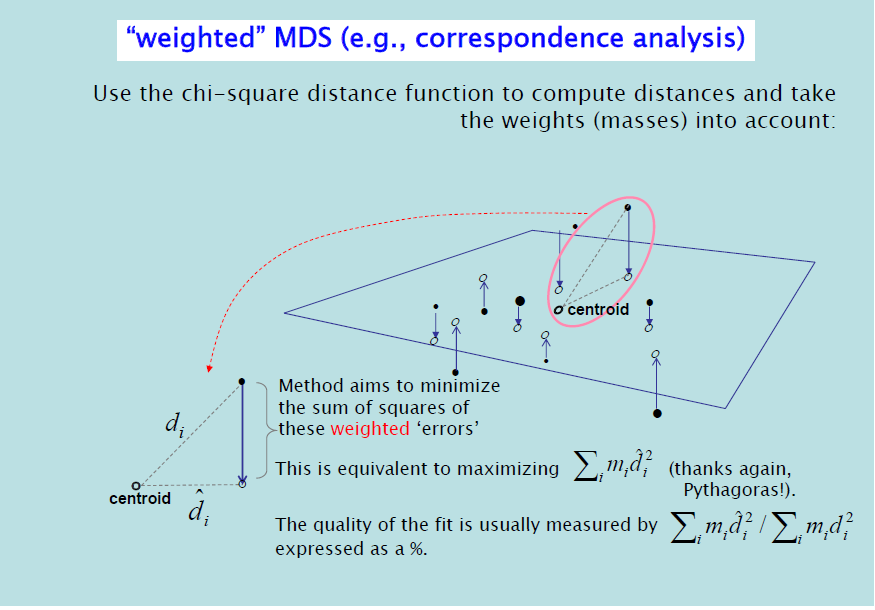
\includegraphics[width=0.7\linewidth]{img/CAquality} 

}

\caption{Pisteen projektio aliavaruuteen}\label{fig:projectionimg1}
\end{figure}

Kuvassa on esitetty korrespondenssianalyysin ratkaisun minimointiongelma. Pisteen
projektio on sitä parempi mitä pienempi kulma on sentroidista pisteeseen
piirtetyn janan ja pisteen projektion välillä. COR - tunnusluku ca-funktion
numeerisissa tuloksissa tämän kulman kosinin neliö. Pisteen kuvauksen laatu (qlt)
ca-tuloksissa on valitun approsimaation akseleiden kvaliteettien (COR) summa.

Kuvasta voi myös hahmottaa sen periaatteen, että projektiossa kaukana olevat
pisteet ovat kaukana myös alkuperäisessä avaruudessa. Projektiossa lähekkäin
olevat pisteet voivat olla alkuperäisessä avaruudessa kaukana toisistaan,
jos niiden projektion laatu on huono.

\hypertarget{matriisit-ja-niiden-havainnollistaminen}{%
\subsection*{Matriisit ja niiden havainnollistaminen}\label{matriisit-ja-niiden-havainnollistaminen}}
\addcontentsline{toc}{subsection}{Matriisit ja niiden havainnollistaminen}

\textbf{edit} Nämä tässä varalla, jos matriisikaavoja tarvitaan lisää. Ehkä ei?

Korrespondenssianalyysin sovelluksissa tutkimusongelman ratkaisu on usein sopivan
matriisin rakentaminen.

\textbf{edit: kaavaesimerkkejä}

\begin{equation}
A = \begin{bmatrix}
    a_{11} & a_{12} & \dots & a_{1k}\\
    \vdots & \ddots & \\
    \\
    \vdots \\
    a_{n1} & \dots  & \dots & a_{nk}
    \end{bmatrix}
\end{equation}

Ehkäpä ABBA onnistuu paremmin tällä notaatiolla?

\begin{equation}
A = \begin{bmatrix}
    A_{11} & B_{12}  \\
    B_{21} & A_{22}
    \end{bmatrix}
\end{equation}

\begin{equation}
A = \begin{bmatrix}
    A_{maa, Q1a} & A_{maa, Q1b}  \\
    B_{gage, Q1a} & B_{gage, Q1b}
    \end{bmatrix}
\end{equation}

\textbf{Pinotut tai yhdistetyt matriisit (``stacked and concatenated matrices'')}

Yksinkertainen korrespondenssianalyysi on kahden luokittelumuuttujan määrittämän
taulukon analyysiä, mutta sitä voi soveltaa myös usean muuttujan analyysiin.
Menetelmän matemaattinen perusta ja ratkaisualgoritmi (SVD) toimivat, tulkinta
vain muuttuu.

Yksinkertaisin laajennus on lisätä alkuperäisen taulukon alle toinen taulukko.
Rivit ovat esimerkissä maittan summattuja vastauksia, ja niiden alle voidaan
lisätä joku toinen luokittelumuuttuja. Havaintojen määrä yhditetyssä (``pinotussa'')
taulussa kaksinkertaistuu.

Taulukoiden yhdistämisen idea on inertian dekomponointi. Yhdistetyn matriisin inertia
voidaan eri tavoin esittää alimatriisien inertian summana. Tällöin jokaisen alimatriisin
reunajakauman tulee olla sama, ja puuttuvat tiedot vääristävät tuloksia.

Merkitään edellisten analyysien kuuden maan ja viiden vastausvaihtoehdon
taulukkoa matriisilla \(\boldsymbol{ A}_{I J}\), missä \(I\) on rivien ja \(J\)
sarakkeiden lukumäärä. Taulukoidaan ikäluokan (1 - 6) ja sukupuolen (\(f\) = nainen,
\(m\) = mies) vuorovaikutusmuuttuja (\(f1,\dots , f6\) ja \(m1,\dots , m6\)) samojen
vastausvaihtoehtojen kanssa. Jos tätä taulukkoa merkitään matriisilla
\(\boldsymbol{ B}_{I^{`} J}\), voimme muodostaa yhdistetyn matriisin

Rivien lukumäärä on molemmissa matriiseissa sama, koska luokkia sattuu olemaan
kuusi sekä maa- että ikä- ja sukupuoli - luokittelumuuttujissa. Kun matriisit
ovat dimensioiltaan ja myös muuttujien sisällön kannalta samankaltaiset, niitä
kutsutaan yhteensopiviksi (``matched matrix''). Tällöin yksinkertaista
korrespondenssianalyyisä voi soveltaa tutkimusongelmaan, jossa halutaan erotella
jonkun ryhmän sisäinen vaihtelu ryhmien välisiestä vaihtelusta.
(Greenacren ehdottama ABBA - analyysi).

ABBA on erityistapaus yleisemmästä moniulotteisen taulukon (multiway table) analyysistä,
jossa useita kahden muuttujan taulukoita ``pinotaan'' päällekkäin ja rinnakkain.
Voimme ottaa yhden kysymyksen vastausten lisäksi analyysiin mukaan useamman
kysymyksen vastaukset laajentamalla kahden päällekkäisen matriisin taulukkoa oikealle.

\textbf{Monimuuttuja-korrespondenssianalyysi MCA}

Usean muuttujan korrespondenssianalyysissä tutkitaan usean muuttujan välisiä yhteyksiä.
Kartan tulkinnan apuna siihen voidaan lisätä havaintojen sijaan niiden keskiarvopisteitä
ja niille simuloituja luottamusellipsejä. Kuvien pääongelma on liian suuri määärä pisteitä,
ja analyysin lopputulos on usein mahdollisimman yksinkertainen kartta.

Usean muuttujan analyysissä kohteena on joko indikaattorimatriisi \(\boldsymbol{Z}\) tai
Burtin matriisi \(\boldsymbol{B}\)

Indikaattorimatriisissa rivit ovat havaintoja ja sarakkeet luokittelumuuttujan arvoja.
Havaintoa vastaa rivi nollia ja arvo 1 valitun vastausvaihtoehdon kohdalla. Tästä seuraa,
että vain erilaiset vastaukset määrittävät rivien etäisyyksiä.

Burtin matriisi on erikoistapaus yhdistetyistä matriiseista. Siihen on koottu kaikki tutkittavien
muuttujien pareittan muodostetut taulukot. Diagonaalilla ovat muuttujien ristiintaulukoinnit
itsensä kanssa. Ratkaisu riippuu vain näistä parittaisista taulukoista.

Burtin matriisi on kätevä välivaihe matriisien yhdistelyssä.

Molemmat matriisit paisuttavat keinotekoisesti kokonaisinertiaa, ja esimerkikisi kaksiulotteisen kartan
selitetyn inertian osuudet jäävät melko pieniksi. Ratkaisuna on inertian oikaisu tai korjaus
(adjusted inertia), jossa mm. poistetaan kokonaisinertialaskelmista Burtin matriisin
diagonaalilla olevat alimatriisit. Näillä korjauksilla ei ole vaikutusta kartan pisteiden
sijaintiin. Tämä menetelmä on ca-paketin mjca-funktion oletus.

Kolmas vaihtoehto on ns. yhdistetty korrespondenssianalyysi (joint ca).

\hypertarget{liite-2-suomenkielinen-lomake-esimerkki}{%
\section*{Liite 2: Suomenkielinen lomake (esimerkki)}\label{liite-2-suomenkielinen-lomake-esimerkki}}
\addcontentsline{toc}{section}{Liite 2: Suomenkielinen lomake (esimerkki)}

Tämä kuva on myös tekstissä, kätevä tapa esittää siististi kysymysten pitkät
versiot.

\begin{Shaded}
\begin{Highlighting}[]
\NormalTok{knitr}\OperatorTok{::}\KeywordTok{include_graphics}\NormalTok{(}\StringTok{'img/substvar_fi_Q1Q2.png'}\NormalTok{)}
\end{Highlighting}
\end{Shaded}

\hypertarget{liite-3-tekninen-ympuxe4ristuxf6-ja-bookdown-paketti}{%
\section*{Liite 3: Tekninen ympäristö ja Bookdown-paketti}\label{liite-3-tekninen-ympuxe4ristuxf6-ja-bookdown-paketti}}
\addcontentsline{toc}{section}{Liite 3: Tekninen ympäristö ja Bookdown-paketti}

Muokataan tiiviimpi pätkä esimerkkireposta bookdown-testi1. Tämä kuva kertoo vain
julkaisutekniikan ympäristön.

\begin{Shaded}
\begin{Highlighting}[]
\NormalTok{knitr}\OperatorTok{::}\KeywordTok{include_graphics}\NormalTok{(}\StringTok{'img/BookdownProc.png'}\NormalTok{)}
\end{Highlighting}
\end{Shaded}

\begin{figure}

{\centering 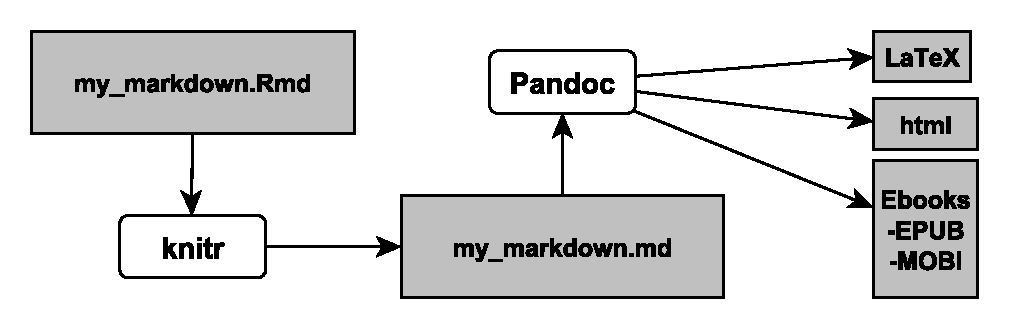
\includegraphics[width=0.7\linewidth]{img/BookdownProc} 

}

\caption{Tulostiedoston prosessointi}\label{fig:L3bdprocess1}
\end{figure}

\begin{Shaded}
\begin{Highlighting}[]
\CommentTok{# pois out.width='50%',}
\end{Highlighting}
\end{Shaded}

\hypertarget{liite-4-r---koodi}{%
\section*{Liite 4: R - koodi}\label{liite-4-r---koodi}}
\addcontentsline{toc}{section}{Liite 4: R - koodi}

\begin{Shaded}
\begin{Highlighting}[]
\CommentTok{# testaukseen 7.11.2020 virheilmoituksia varten arvo TRUE}
\KeywordTok{options}\NormalTok{(}\DataTypeTok{tinytex.verbose =} \OtherTok{TRUE}\NormalTok{)}

\CommentTok{# 18.10.2020}
\KeywordTok{library}\NormalTok{(rgl)}
\KeywordTok{library}\NormalTok{(ca)}
\KeywordTok{library}\NormalTok{(haven)}
\KeywordTok{library}\NormalTok{(dplyr)}
\KeywordTok{library}\NormalTok{(knitr)}
\KeywordTok{library}\NormalTok{(tidyverse)}
\KeywordTok{library}\NormalTok{(lubridate)}
\KeywordTok{library}\NormalTok{(rmarkdown)}
\KeywordTok{library}\NormalTok{(ggplot2)}
\KeywordTok{library}\NormalTok{(furniture)}
\KeywordTok{library}\NormalTok{(scales) }\CommentTok{# G_1_2 - kuva}
\KeywordTok{library}\NormalTok{(reshape2)  }\CommentTok{# G_1_2 - kuva}
\KeywordTok{library}\NormalTok{(printr) }\CommentTok{#19.5.18 taulukoiden ja matriisien tulostukseen}
\KeywordTok{library}\NormalTok{(bookdown)}
\KeywordTok{library}\NormalTok{(tinytex)}
\KeywordTok{library}\NormalTok{(assertthat)}


\CommentTok{# automatically create a bib database for R packages}
\NormalTok{knitr}\OperatorTok{::}\KeywordTok{write_bib}\NormalTok{(}\KeywordTok{c}\NormalTok{(}
  \KeywordTok{.packages}\NormalTok{(), }\StringTok{'bookdown'}\NormalTok{, }\StringTok{'knitr'}\NormalTok{, }\StringTok{'rmarkdown'}
\NormalTok{), }\StringTok{'packages.bib'}\NormalTok{)}

\CommentTok{# include FALSE: ei koodia eikä tulostusta dokumenttiin - poistettava turhia}
\CommentTok{# välitulostuksia (18.10.2020)}
\CommentTok{# Aineiston rajaamisen kolme vaihetta (10.2018)}
\CommentTok{# }
\CommentTok{# TIEDOSTOJEN NIMEÄMINEN}
\CommentTok{#}
\CommentTok{# R-datatiedostot .data - tarkenteella ovat osajoukkoja koko ISSP-datasta ISSP2012.data}
\CommentTok{# R-datatiedostot .dat - tarkenteella: mukana alkuperäisten muuttujien muunnoksia }
\CommentTok{# (yleensä as_factor), alkuperäisissä muuttujissa mukana SPSS-tiedoston metadata.}
\CommentTok{#}
\CommentTok{# Luokittelumuuttujan tyyppi on datan lukemisen jälkeen yleensä merkkijono (char) }
\CommentTok{# ja haven_labelled. }
\CommentTok{#}
\CommentTok{# Muutetaan R-datassa ordinaali- tai  nominaaliasteikon muuttujat haven-paketin }
\CommentTok{# as_factor - funktiolla faktoreiksi. R:n faktorityypin muuttujille voidaan tarvittaessa }
\CommentTok{# määritellä järjestys, toistaiseksi niin ei tehdä (25.9.2018). }
\CommentTok{#}
\CommentTok{# Muunnetun muuttujan rinnalla säilytetään SPSS-tiedostosta luettu muuttja, metatiedot säilyvät }
\CommentTok{# alkuperäisessä.}
\CommentTok{#       }
\CommentTok{# R-datatiedostot joiden nimen loppuosa on muotoa *esim1.dat: käytetään analyyseissä}
\CommentTok{#}
\CommentTok{# 1. VALITAAN MAAT (25) -> ISSP2012jh1a.data. Muuttujat koodilohkossa datasel_vars1}
\CommentTok{#}
\CommentTok{# kolme maa-muuttujaa datassa. V3 erottelee joidenkin maiden alueita, V4 on koko }
\CommentTok{# maan koodi ja C_ALPHAN on maan kaksimerkkinen tunnus.}
\CommentTok{#}
\CommentTok{# V3 - Country/ Sample ISO 3166 Code (see V4 for codes for whole nation states)}
\CommentTok{# V3 erot valituissa maissa}
\CommentTok{# 5601 BE-FLA-Belgium/ Flanders}
\CommentTok{# 5602 BE-WAL-Belgium/ Wallonia}
\CommentTok{# 5603 BE-BRU-Belgium/ Brussels}
\CommentTok{# 27601 DE-W-Germany-West}
\CommentTok{# 27602 DE-E-Germany-East}
\CommentTok{# 62001 PT-Portugal 2012: first fieldwork round (main sample)}
\CommentTok{# 62002 PT-Portugal 2012: second fieldwork round (complementary sample)}
\CommentTok{# Myös tämä on erikoinen, näyttää olevan vakio kun V4 = 826:}
\CommentTok{# 82601 GB-GBN-Great Britain}
\CommentTok{# Portugalissa ainestoa täydennettiin, koska siinä oli puutteita. Jako ei siis ole oleellinen,}
\CommentTok{# mutta muuut ovat. Tähdellä merkityt maat valitaan johdattelevaan esimerkkiin.}
\CommentTok{#}
\CommentTok{# Maat (25)}
\CommentTok{#}
\CommentTok{# 36 AU-Australia}
\CommentTok{# 40 AT-Austria}
\CommentTok{# 56 BE-Belgium*}
\CommentTok{# 100 BG-Bulgaria*}
\CommentTok{# 124 CA-Canada}
\CommentTok{# 191 HR-Croatia}
\CommentTok{# 203 CZ-Czech Republic}
\CommentTok{# 208 DK-Denmark*}
\CommentTok{# 246 FI-Finland*}
\CommentTok{# 250 FR-France}
\CommentTok{# 276 DE-Germany*}
\CommentTok{# 348 HU-Hungary*}
\CommentTok{# 352 IS-Iceland}
\CommentTok{# 372 IE-Ireland}
\CommentTok{# 428 LV-Latvia}
\CommentTok{# 440 LT-Lithuania}
\CommentTok{# 528 NL-Netherlands}
\CommentTok{# 578 NO-Norway}
\CommentTok{# 616 PL-Poland}
\CommentTok{# 620 PT-Portugal}
\CommentTok{# 643 RU-Russia}
\CommentTok{# 703 SK-Slovakia}
\CommentTok{# 705 SI-Slovenia}
\CommentTok{# 752 SE-Sweden}
\CommentTok{# 756 CH-Switzerland}
\CommentTok{# 826 GB-Great Britain and/or United Kingdom - jätetään pois jotta saadaan TOPBOT }
\CommentTok{#                          -muuttuja mukaan (top-bottom self-placement) .(9.10.18)}
\CommentTok{# 840 US-United States - jätetään pois, jotta saadaan TOPBOT-muuttuja mukaan.(10.10.18)}
\CommentTok{#}
\CommentTok{# Belgian ja Saksan alueet:}
\CommentTok{#  V3}
\CommentTok{#  5601     BE-FLA-Belgium/ Flanders}
\CommentTok{#  5602     BE-WAL-Belgium/ Wallonia}
\CommentTok{#  5603     BE-BRU-Belgium/ Brussels}
\CommentTok{# 27601     DE-W-Germany-West}
\CommentTok{# 27602     DE-E-Germany-East}
\CommentTok{#}
\CommentTok{# Unkari (348) toistaiseksi mukana, mutta joissain kysymyksissä myös Unkarilla on }
\CommentTok{# poikkeavia vastausvaihtoehtoja(HU_V18, HU_V19,HU_V20). Jos näitä muuttujia käytetään, }
\CommentTok{# Unkari on parempi jättää pois. }
\CommentTok{# }
\CommentTok{#}
\CommentTok{# (25.4.2018) user_na  }
\CommentTok{# haven-paketin read_spss - funktiolla voi r-tiedostoon lukea myös SPSS:n sallimat kolme }
\CommentTok{# (yleensä 7, 8, 9) tarkempaa koodia puuttuvalle tiedolle.}
\CommentTok{# "If TRUE variables with user defined missing will be read into labelled_spss objects. }
\CommentTok{# If FALSE, the default, user-defined missings will be converted to NA"}
\CommentTok{# https://www.rdocumentation.org/packages/haven/versions/1.1.0/topics/read_spss}
\CommentTok{#}
 
\NormalTok{ISSP2012jh.data <-}\StringTok{ }\KeywordTok{read_spss}\NormalTok{(}\StringTok{"data/ZA5900_v4-0-0.sav"}\NormalTok{) }\CommentTok{#luetaan alkuperäinen data R- dataksi (df).}

\CommentTok{#str(ISSP2012jh.data)}

\NormalTok{incl_countries25 <-}\StringTok{ }\KeywordTok{c}\NormalTok{(}\DecValTok{36}\NormalTok{, }\DecValTok{40}\NormalTok{, }\DecValTok{56}\NormalTok{,}\DecValTok{100}\NormalTok{, }\DecValTok{124}\NormalTok{, }\DecValTok{191}\NormalTok{, }\DecValTok{203}\NormalTok{, }\DecValTok{208}\NormalTok{, }\DecValTok{246}\NormalTok{, }\DecValTok{250}\NormalTok{, }\DecValTok{276}\NormalTok{, }\DecValTok{348}\NormalTok{, }\DecValTok{352}\NormalTok{, }
                      \DecValTok{372}\NormalTok{, }\DecValTok{428}\NormalTok{, }\DecValTok{440}\NormalTok{, }\DecValTok{528}\NormalTok{, }\DecValTok{578}\NormalTok{, }\DecValTok{616}\NormalTok{, }\DecValTok{620}\NormalTok{, }\DecValTok{643}\NormalTok{, }\DecValTok{703}\NormalTok{, }\DecValTok{705}\NormalTok{, }\DecValTok{752}\NormalTok{, }\DecValTok{756}\NormalTok{)}

\CommentTok{#str(ISSP2012jh.data)}
\CommentTok{#str(ISSP2012jh.data) #61754 obs. of  420 variables - kaikki}

\NormalTok{ISSP2012jh1a.data <-}\StringTok{ }\KeywordTok{filter}\NormalTok{(ISSP2012jh.data, V4 }\OperatorTok\StringTok{ }\NormalTok{incl_countries25)}

\CommentTok{#head(ISSP2012jh1a.data)}
\CommentTok{#str(ISSP2012jh1a.data) #34271 obs. of  420 variables, Espanja ja Iso-Britannia}
\CommentTok{#                       pois (9.10.2018)}
\CommentTok{# str(ISSP2012jh1a.data) # 32969 obs. of  420 variable, Espanja Iso-Britannia, }
\CommentTok{#                        USA pois (10.10.2018)}
\CommentTok{#}
\CommentTok{# names() # muuttujen nimet}
\CommentTok{# Maakohtaiset muuttujat (kun on poikettu ISSP2012 - vastausvaihtoehdoista tms.) }
\CommentTok{# on aineistossa eroteltu maatunnus-etuliitteellä (esimerkiksi ES_V7).}
\CommentTok{# Demografisissa ja muissa taustamuuttujissa suuri osa tiedoista on kerätty maa-}
\CommentTok{# kohtaisilla lomakkeilla. Vertailukelpoiset muuttujat on konstruoitu niistä.}
\CommentTok{# Muuttujia on 420, vain osa yhteisiä kaikille maille.}

\CommentTok{# include FALSE: ei koodia eikä tulostusta dokumenttiin - poistettava turhia}
\CommentTok{# välitulostuksia (18.10.2020)}
\CommentTok{# 2. VALITAAN MUUTTUJAT  -> ISSP2012jh1b.data. Maat valittu koodilohkossa datasel_country1}
\CommentTok{#}
\CommentTok{#}
\CommentTok{# Muuttujat on luokiteltu dokumentissa ZA5900_overview.pdf}
\CommentTok{# https://zacat.gesis.org/webview/index.jsp?object=http://zacat.gesis.org/obj/fStudy/ZA5900}
\CommentTok{# Study Description -> Other Study Description -> Related Materials}
\CommentTok{# }
\CommentTok{#}

\CommentTok{# METADATA}

\NormalTok{metavars1 <-}\StringTok{ }\KeywordTok{c}\NormalTok{(}\StringTok{"V1"}\NormalTok{, }\StringTok{"V2"}\NormalTok{, }\StringTok{"DOI"}\NormalTok{)}

\CommentTok{#MAA - maakoodit ja maan kahden merkin tunnus}

\NormalTok{countryvars1 <-}\StringTok{ }\KeywordTok{c}\NormalTok{(}\StringTok{"V3"}\NormalTok{,}\StringTok{"V4"}\NormalTok{,}\StringTok{"C_ALPHAN"}\NormalTok{)}

\CommentTok{# SUBSTANSSIMUUTTUJAT - Attitudes towards family and gender roles (9)}
\CommentTok{#}
\CommentTok{# Yhdeksän kysymystä (lyhennetyt versiot, englanniksi), vastausvaihtoehdot Q1-Q2}
\CommentTok{#}
\CommentTok{# 1 = täysin samaa mieltä, 2 = samaa mieltä, 3 = ei samaa eikä eri mieltä, }
\CommentTok{# 4 = eri mieltä, 5 = täysin eri mieltä}
\CommentTok{# }
\CommentTok{# Q1a Working mother can have warm relation with child}
\CommentTok{# Q1b Pre-school child suffers through working mother}
\CommentTok{# Q1c Family life suffers through working mother}
\CommentTok{# Q1d Women’s preference: home and children}
\CommentTok{# Q1e Being housewife is satisfying}
\CommentTok{#}
\CommentTok{# Q2a Both should contribute to household income}
\CommentTok{# Q2b Men’s job is earn money, women’s job household}
\CommentTok{#}
\CommentTok{# Q3a Should women work: Child under school age }
\CommentTok{# Q3b Should women work: Youngest kid at school}
\CommentTok{# 1= kokopäivätyö, 2 = osa-aikatyö, 3 = pysyä kotona, 8 = en osaa sanoa}
\CommentTok{# (can't choose), 9 = no answer}
\CommentTok{#}
\CommentTok{# Kysymysten Q3a ja Q3b eos-vastaus ei ole sama kuin "en samaa enkä eri  mieltä"}
\CommentTok{# (ns. neutraali # vaihtoehto), mutta kieltäytymisiä jne. (koodi 9) on aika}
\CommentTok{# vähän. Kolmessa # maassa ne on yhdistety: }
\CommentTok{# (8 Can't choose, CA:can't choose+no answer, KR:don't know+refused, NL:don't know).}
\CommentTok{# Kun SPSS-tiedostosta ei ole tuotu puuttuvan tiedon tarkempaa luokittelua,}
\CommentTok{# erottelua ei voi tehdä.}
\CommentTok{#}

\NormalTok{substvars1 <-}\StringTok{ }\KeywordTok{c}\NormalTok{(}\StringTok{"V5"}\NormalTok{,}\StringTok{"V6"}\NormalTok{,}\StringTok{"V7"}\NormalTok{,}\StringTok{"V8"}\NormalTok{,}\StringTok{"V9"}\NormalTok{,}\StringTok{"V10"}\NormalTok{,}\StringTok{"V11"}\NormalTok{,}\StringTok{"V12"}\NormalTok{,}\StringTok{"V13"}\NormalTok{) }\CommentTok{# 9 muuttujaa}

\CommentTok{# Nämä yhteiset muuttujat pois (maaspesifien muuttujien lisäksi) :}
\CommentTok{#}
\CommentTok{# "V14","V15","V16",  "V17","V18","HU_V18","V19","HU_V19","V20","HU_V20","V21",}
\CommentTok{# "V28","V29","V30","V31","V32","V33",# "V34", "V35", "V36", "V37", "V38", "V39",}
\CommentTok{# "V40", "V41", "V42", "V43", "V44", "V45", "V46", "V47", "V48", "V49", "V50", }
\CommentTok{# "V51", "V52", "V53", "V54", "V55", "V56", "V57", "V58", "V59", "V60", "V61", }
\CommentTok{# "V62", "V63", "V64", "V65", "V65a","V66", "V67"}
\CommentTok{#}
\CommentTok{#}
\CommentTok{# DEMOGRAFISET JA MUUT TAUSTAMUUTTUJAT (8)}
\CommentTok{#}
\CommentTok{# AGE, SEX}
\CommentTok{#}
\CommentTok{# DEGREE - Highest completed degree of education: Categories for international}
\CommentTok{# comparison. Slightly re-arranged subset of ISCED-97}
\CommentTok{#}
\CommentTok{# 0 No formal education}
\CommentTok{# 1 Primary school (elementary school)}
\CommentTok{# 2 Lower secondary (secondary completed does not allow entry to university:}
\CommentTok{#  obligatory school)}
\CommentTok{# 3 Upper secondary (programs that allow entry to university or programs that}
\CommentTok{#  allow to entry other ISCED level 3 programs - designed to prepare students for}
\CommentTok{#  direct entry into the labour market)}
\CommentTok{# 4 Post secondary, non-tertiary (other upper secondary programs toward labour}
\CommentTok{#  market or technical formation)}
\CommentTok{# 5 Lower level tertiary, first stage (also technical schools at a tertiary level)}
\CommentTok{# 6 Upper level tertiary (Master, Dr.)}
\CommentTok{# 9 No answer, CH: don't know}
\CommentTok{# HUOM! R-factor - muunnoksessa koodaus on 1-7}
\CommentTok{#}
\CommentTok{# MAINSTAT - main status: Which of the following best describes your current situation?}
\CommentTok{#}
\CommentTok{# 1 In paid work}
\CommentTok{# 2 Unemployed and looking for a job, HR: incl never had a job}
\CommentTok{# 3 In education}
\CommentTok{# 4 Apprentice or trainee}
\CommentTok{# 5 Permanently sick or disabled}
\CommentTok{# 6 Retired}
\CommentTok{# 7 Domestic work}
\CommentTok{# 8 In compulsory military service or community service}
\CommentTok{# 9 Other}
\CommentTok{# 99 No answer}
\CommentTok{# Armeijassa tai yhdyskuntapalvelussa muutamia, muutamissa maissa.Kategoriassa 9 }
\CommentTok{# on hieman väkeä. Yhdistetään 8 ja 9. Huom! Esim Puolassa ei yhtään eläkeläistä}
\CommentTok{# eikä kategoriaa 9, Saksassa ei ketään kategoriassa 9.}
\CommentTok{#}
\CommentTok{# TOPBOT - Top-Bottom self-placement (10 pt scale)}
\CommentTok{#}
\CommentTok{# "In our society, there are groups which tend to be towards the top and groups }
\CommentTok{# which tend to be towards the bottom. Below is a scale that runs}
\CommentTok{# from the top to the bottom. Where would you put yourself on this scale?"}
\CommentTok{# Eri maissa hieman erilaisia kysymyksiä. }
\CommentTok{#}
\CommentTok{# HHCHILDR - How many children in household: children between [school age] and}
\CommentTok{# 17 years of age}
\CommentTok{#}
\CommentTok{# 0 No children}
\CommentTok{# 1 One child}
\CommentTok{# 2 2 children}
\CommentTok{# 21 21 children}
\CommentTok{# 96 NAP (Code 0 in HOMPOP)}
\CommentTok{# 97 Refused}
\CommentTok{# 99 No answer}
\CommentTok{#}
\CommentTok{# Voisi koodata dummymuuttujaksi lapsia (1) - ei lapsia (0).}
\CommentTok{# Ranskan datassa on erittäin iso osa puuttuvia tietoja (yli 20 %), Sama tilanne}
\CommentTok{# myös  muissa perheen kokoon liittyvissä kysymyksissä.  Myös Austarlialla aika}
\CommentTok{# paljon puuttuvia vastauksia.}
\CommentTok{#}
\CommentTok{# MARITAL - Legal partnership status }
\CommentTok{#}
\CommentTok{# What is your current legal marital status?}
\CommentTok{# The aim of this variable is to measure the current 'legal' marital status '. }
\CommentTok{# PARTLIV - muuttujassa on 'de facto' - tilanteen tieto parisuhteesta}
\CommentTok{#}
\CommentTok{# 1 Married}
\CommentTok{# 2 Civil partnership}
\CommentTok{# 3 Separated from spouse/ civil partner (still legally married/ still legally }
\CommentTok{#   in a civil partnership)}
\CommentTok{# 4 Divorced from spouse/ legally separated from civil partner}
\CommentTok{# 5 Widowed/ civil partner died}
\CommentTok{# 6 Never married/ never in a civil partnership, single}
\CommentTok{# 7 Refused}
\CommentTok{# 8 Don't know}
\CommentTok{# 9 No answer}
\CommentTok{#}
\CommentTok{# URBRURAL - Place of living: urban - rural}
\CommentTok{#}
\CommentTok{# 1 A big city}
\CommentTok{# 2 The suburbs or outskirts of a big city}
\CommentTok{# 3 A town or a small city}
\CommentTok{# 4 A country village}
\CommentTok{# 5 A farm or home in the country}
\CommentTok{# 7 Other answer}
\CommentTok{# 9 No answer}
\CommentTok{# 1 ja 2 vaihtelevat aika paljon maittain, parempi laskea yhteen. Unkarista puuttuu }
\CommentTok{# jostain syystä kokonaan vaihtoehto 5.  Vaihotehdon 7 on valinnut vain 4}
\CommentTok{# vastaajaa Ranskasta.}
\CommentTok{#}

\NormalTok{bgvars1 <-}\StringTok{ }\KeywordTok{c}\NormalTok{( }\StringTok{"SEX"}\NormalTok{,}\StringTok{"AGE"}\NormalTok{,}\StringTok{"DEGREE"}\NormalTok{, }\StringTok{"MAINSTAT"}\NormalTok{, }\StringTok{"TOPBOT"}\NormalTok{,}
              \StringTok{"HHCHILDR"}\NormalTok{, }\StringTok{"MARITAL"}\NormalTok{, }\StringTok{"URBRURAL"}\NormalTok{)}

\CommentTok{#Valitaan muuttujat}

\NormalTok{jhvars1 <-}\StringTok{ }\KeywordTok{c}\NormalTok{(metavars1,countryvars1, substvars1,bgvars1)}

\CommentTok{#jhvars1}
\NormalTok{ISSP2012jh1b.data <-}\StringTok{ }\KeywordTok{select}\NormalTok{(ISSP2012jh1a.data, }\KeywordTok{all_of}\NormalTok{(jhvars1)) }

\CommentTok{# laaja aineisto - mukana havainnot joissa puuttuvia tietoja}
\CommentTok{# str(ISSP2012jh1b.data) #32969 obs. of  23 variables }
\CommentTok{# }
\CommentTok{# SUBSTANSSIMUUTTUJAT}
\CommentTok{#}
\CommentTok{# $ V5      : 'haven_labelled' num  5 1 2 2 1 NA 2 4 2 2 ...}
\CommentTok{#  ..- attr(*, "label")= chr "Q1a Working mom: warm relationship with children}
\CommentTok{#       as a not working mom"}
\CommentTok{#  ..- attr(*, "labels")= Named num  0 1 2 3 4 5 8 9}
\CommentTok{#}
\CommentTok{# ISSP2012jh1b.data$V5 näyttää tarkemmin rakenteen}
\CommentTok{#}
\CommentTok{# glimpse(ISSP2012jh1b.data)}

\CommentTok{# Poistetaan havainnot, joissa ikä (AGE) tai sukupuolitieto puuttuu (5.7.2019)}

\NormalTok{ISSP2012jh1c.data <-}\StringTok{ }\KeywordTok{filter}\NormalTok{(ISSP2012jh1b.data, (}\OperatorTok{!}\KeywordTok{is.na}\NormalTok{(SEX) }\OperatorTok{&}\StringTok{ }\OperatorTok{!}\KeywordTok{is.na}\NormalTok{(AGE)))}

\CommentTok{# str(ISSP2012jh1c.data) # 32823 obs. of  23 variables, 32969-32823 = 146}
\CommentTok{# TARKISTUS 8.6.20 dplyr 1.0.0-päivitys: havaintojen ja muuttujien määrä ok.}

\CommentTok{# VAIHE 1 - muuttujat joissa ei ole puuttuvia tietoja}

\CommentTok{# vaihe 1.1 haven_labelled ja chr -> as_factor}

\NormalTok{ISSP2012jh1d.dat <-}\StringTok{ }\NormalTok{ISSP2012jh1c.data }\OperatorTok
\StringTok{    }\KeywordTok{mutate}\NormalTok{(}\DataTypeTok{maa =} \KeywordTok{as_factor}\NormalTok{(C_ALPHAN), }\CommentTok{# ei puuttuvia, ei tyhjiä leveleitä}
           \DataTypeTok{maa3 =} \KeywordTok{as_factor}\NormalTok{(V3),  }\CommentTok{# maakoodi, jossa aluejako joillan mailla}
           \DataTypeTok{sp1 =} \KeywordTok{as_factor}\NormalTok{(SEX), }\CommentTok{# ei puuttuvia, tyhjä level "no answer" 999}
\NormalTok{         )}


\CommentTok{# C_ALPHAN - maa - maa3 tarkistuksia}

\CommentTok{# V3}
\CommentTok{# "Pulma" on järjestys. C_ALPHAN ("chr") on aakkosjärjestyksessä, kun luodaan}
\CommentTok{# maa = as_factor(C_ALPHAN) järjestys muuttuu (esiintymisjärjestys datassa?)}
\CommentTok{# maa3 muunnetaan maakoodista (haven_labelled' num), jonka}

\CommentTok{# str(ISSP2012jh1d.dat$maa) #Country Prefix ISO 3166 Code - alphanumeric}
\CommentTok{# attributes(ISSP2012jh1d.dat$maa) # ei tyhiä levels-arvoja, 25 levels}
\CommentTok{# ISSP2012jh1d.dat$maa %>% fct_unique()}
\CommentTok{# ISSP2012jh1d.dat$maa %>% fct_count() # summary kertoo samat tiedot (20.2.20)}
\CommentTok{# sum(is.na(ISSP2012jh1d.dat$maa)) # ei puuttuvia tietoja}
\CommentTok{# ISSP2012jh1d.dat$maa %>% summary() # mukana vain valitut 25 maata}

\CommentTok{# str(ISSP2012jh1d.dat$maa3)  #"Country/ Sample ISO 3166 Code}
                            \CommentTok{#(see V4 for codes for whole nation states)"}
                            \CommentTok{# 29 levels}
\CommentTok{# str(ISSP2012jh1d.dat$V3)}

\CommentTok{# attributes(ISSP2012jh1d.dat$maa3) # ei tyhiä levels-arvoja, 29 levels}
\CommentTok{# sum(is.na(ISSP2012jh1d.dat$maa3)) # nolla ei ole puuttuva tieto! (3.2.20)}
\CommentTok{# ISSP2012jh1d.dat$maa3 %>% fct_unique()}
\CommentTok{# ISSP2012jh1d.dat$maa3 %>% fct_count()}
\CommentTok{# Vain näissä on jaettu maan havainnot (3.2.20)}
\CommentTok{#}
\CommentTok{# [38] BE-FLA-Belgium/ Flanders}
\CommentTok{# [39] BE-WAL-Belgium/ Wallonia}
\CommentTok{# [40] BE-BRU-Belgium/ Brussels}
\CommentTok{# [41] DE-W-Germany-West}
\CommentTok{# [42] DE-E-Germany-East}
\CommentTok{# [43] PT-Portugal 2012: first fieldwork round (main sample)}
\CommentTok{# [44] PT-Portugal 2012: second fieldwork round (complementary sample)}

\CommentTok{# ISSP2012jh1d.dat$maa3 %>% fct_count() #miksi ei tulosta mitään? (3.2.2020)}

\CommentTok{# ISSP2012jh1d.dat$maa3 %>% summary()}
\CommentTok{# ISSP2012jh1d.dat$maa3 %>% fct_unique()}
\CommentTok{# maa3: 25 maata, havaintojen määrä. Poisjätetyissä havaintoja 0.}
\CommentTok{# glimpse(ISSP2012jh1d.dat$maa3)}
\CommentTok{# head(ISSP2012jh1d.dat$maa3)}
\CommentTok{# length(levels(ISSP2012jh1d.dat$maa3))}

\CommentTok{# C_ALPHAN alkuperäinen järjestys, maa aakkosjärjestyssä  (2.2.20)}
\CommentTok{#}
\CommentTok{# Huom1: Myös merkkijonomuuttujaa C_ALPHAN tarvitaan jatkossa.}
\CommentTok{#}
\CommentTok{# Huom2: kun dataa rajataan, on tarkistettava ja tarvittaessa poistettava}
\CommentTok{# "tyhjät" R-factor - muuttujan "maa" luokat (3.2.2020)}


\CommentTok{# vaihe 1.2 tyhjät luokat (levels) pois faktoreista}

\NormalTok{ISSP2012jh1d.dat <-}\StringTok{ }\NormalTok{ISSP2012jh1d.dat }\OperatorTok
\StringTok{    }\KeywordTok{mutate}\NormalTok{(}\DataTypeTok{sp =} \KeywordTok{fct_drop}\NormalTok{(sp1),}
           \DataTypeTok{maa3 =} \KeywordTok{fct_drop}\NormalTok{(maa3)}
\NormalTok{           )}

\CommentTok{#  maa3 - tarkistuksia}

\CommentTok{# str(ISSP2012jh1d.dat$maa3)  # 29 levels}
\CommentTok{# attributes(ISSP2012jh1d.dat$maa3)}
\CommentTok{#sum(is.na(ISSP2012jh1d.dat$maa3)) # nolla ei ole puuttuva tieto! (3.2.20)}
\CommentTok{# ISSP2012jh1d.dat$maa3 %>% summary()}
\CommentTok{# ISSP2012jh1d.dat$maa3 %>% fct_unique()}
\CommentTok{# ISSP2012jh1d.dat$maa3 %>% fct_count()}
\CommentTok{#}
\CommentTok{# str(ISSP2012jh1d.dat$C_ALPHAN)}
\CommentTok{# attributes(ISSP2012jh1d.dat$C_ALPHAN)}

\CommentTok{# TESTAUKSIA}
\CommentTok{# }
\CommentTok{# ISSP2012jh1d.dat %>% tableX(C_ALPHAN, maa)}
\CommentTok{# ISSP2012jh1d.dat %>% tableX(C_ALPHAN, maa3)}
\CommentTok{# ISSP2012jh1d.dat %>% tableX(maa, maa3)}
\CommentTok{# ISSP2012jh1d.dat %>% tableX(V3, maa3)}

\CommentTok{# sp, sp1, SEX - tarkistuksia}
\CommentTok{# }
\CommentTok{# ISSP2012jh1d.dat$sp %>% fct_count()}
\CommentTok{# ISSP2012jh1d.dat$sp %>% fct_count()}
\CommentTok{# ISSP2012jh1d.dat %>% tableX(SEX,sp1)}
\CommentTok{# ISSP2012jh1d.dat %>% tableX(SEX,sp)}
\CommentTok{# ISSP2012jh1d.dat %>% tableX(sp1,sp)}

\CommentTok{# vaihe 1.3 uudet "faktorilabelit"}
\NormalTok{ISSP2012jh1d.dat <-}\StringTok{ }\NormalTok{ISSP2012jh1d.dat }\OperatorTok
\StringTok{    }\KeywordTok{mutate}\NormalTok{(}\DataTypeTok{sp =}
          \KeywordTok{fct_recode}\NormalTok{(sp,}
            \StringTok{"m"}\NormalTok{ =}\StringTok{ "Male"}\NormalTok{,}
            \StringTok{"f"}\NormalTok{ =}\StringTok{ "Female"}\NormalTok{)}
\NormalTok{            )}

\CommentTok{# Tarkistuksia}

\CommentTok{# ISSP2012jh1d.dat$sp %>% fct_unique()}
\CommentTok{# ISSP2012jh1d.dat$sp %>% fct_count()}
\CommentTok{# ISSP2012jh1d.dat$sp %>% summary()}

\CommentTok{# AGE -> ika}
\NormalTok{ISSP2012jh1d.dat}\OperatorTok{$}\NormalTok{ika <-}\StringTok{ }\NormalTok{ISSP2012jh1d.dat}\OperatorTok{$}\NormalTok{AGE}

\CommentTok{# Tarkistuksia}
\KeywordTok{attributes}\NormalTok{(ISSP2012jh1d.dat}\OperatorTok{$}\NormalTok{ika) }\CommentTok{# tyhjä level "No answer"}
\CommentTok{# str(ISSP2012jh1d.dat$ika)}
\NormalTok{ISSP2012jh1d.dat}\OperatorTok{$}\NormalTok{ika }\OperatorTok\StringTok{ }\KeywordTok{summary}\NormalTok{()}

\NormalTok{ISSP2012jh1d.dat }\OperatorTok
\KeywordTok{tableC}\NormalTok{(AGE, ika,}\DataTypeTok{cor_type =} \StringTok{"pearson"}\NormalTok{, }\DataTypeTok{na.rm =} \OtherTok{FALSE}\NormalTok{, }\DataTypeTok{rounding =} \DecValTok{5}\NormalTok{,}
       \DataTypeTok{output =} \StringTok{"text"}\NormalTok{, }\DataTypeTok{booktabs =} \OtherTok{TRUE}\NormalTok{, }\DataTypeTok{caption =} \OtherTok{NULL}\NormalTok{, }\DataTypeTok{align =} \OtherTok{NULL}\NormalTok{,}
       \DataTypeTok{float =} \StringTok{"htb"}\NormalTok{) }\OperatorTok\StringTok{ }\KeywordTok{kable}\NormalTok{()}

\CommentTok{# Ikäjakauma - ei tarvita (18.10.2020)}
\CommentTok{#}
\CommentTok{# ISSP2012jh1d.dat$ika %>% hist(main = "ISSP 2012: vastaajan ikä")}

\CommentTok{# Substanssi- ja taustamuuttujat R-faktoreiksi}
\NormalTok{ISSP2012jh1d.dat <-}\StringTok{ }\NormalTok{ISSP2012jh1d.dat }\OperatorTok
\StringTok{    }\KeywordTok{mutate}\NormalTok{(}\DataTypeTok{Q1a1 =} \KeywordTok{as_factor}\NormalTok{(V5), }\CommentTok{#labels}
            \DataTypeTok{Q1b1 =} \KeywordTok{as_factor}\NormalTok{(V6),}
            \DataTypeTok{Q1c1 =} \KeywordTok{as_factor}\NormalTok{(V7),}
            \DataTypeTok{Q1d1 =} \KeywordTok{as_factor}\NormalTok{(V8),}
            \DataTypeTok{Q1e1 =} \KeywordTok{as_factor}\NormalTok{(V9),}
            \DataTypeTok{Q2a1 =} \KeywordTok{as_factor}\NormalTok{(V10),}
            \DataTypeTok{Q2b1 =} \KeywordTok{as_factor}\NormalTok{(V11),}
            \DataTypeTok{Q3a1 =} \KeywordTok{as_factor}\NormalTok{(V12), }\CommentTok{#labels = vastQ3_labels (W,w,H)}
            \DataTypeTok{Q3b1 =} \KeywordTok{as_factor}\NormalTok{(V13), }\CommentTok{#labels = vastQ3_labels}
            \DataTypeTok{edu1 =} \KeywordTok{as_factor}\NormalTok{(DEGREE),}
            \DataTypeTok{msta1 =} \KeywordTok{as_factor}\NormalTok{(MAINSTAT),}
            \DataTypeTok{sosta1 =} \KeywordTok{as_factor}\NormalTok{(TOPBOT),}
            \DataTypeTok{nchild1 =} \KeywordTok{as_factor}\NormalTok{(HHCHILDR),}
            \DataTypeTok{lifsta1 =} \KeywordTok{as_factor}\NormalTok{(MARITAL),}
            \DataTypeTok{urbru1 =} \KeywordTok{as_factor}\NormalTok{(URBRURAL)}
\NormalTok{           )}

\CommentTok{# Muuttujat Q1a1...urbru1 ovat apumuuttujia, joissa on periaatteessa kaikki SPSS-}
\CommentTok{# tiedostosta siirtyvä metatieto. Poikkeus on SPSS:n kolme tarkentavaa koodia}
\CommentTok{# puuttuvalle tiedolle, ne saisi mukaan read_spss - parametrin avulla (user_na=TRUE)}
\CommentTok{#}

\CommentTok{# Tarkistusksia}
\CommentTok{# ISSP2012jh1d.dat %>% summary()}

\CommentTok{# ISSP2012jh1d.dat %>%}
\CommentTok{#    select(Q1a1, Q1b1, Q1c1,Q1d1,Q1e1, Q2a1, Q2b1, Q3a1,Q3b1) %>%}
\CommentTok{#    summary()}
\CommentTok{#}
\CommentTok{# ISSP2012jh1d.dat %>%}
\CommentTok{#    select(edu1,msta1, sosta1, nchild1, lifsta1, urbru1) %>%}
\CommentTok{#    summary()}


\CommentTok{# Substanssimuuttujat - ristiintaulukoinnit riittävät (6.2.20)}

\CommentTok{# ISSP2012jh1d.dat$Q1a1 %>% fct_count()}
\CommentTok{# ISSP2012jh1d.dat$Q1b1 %>% fct_count()}
\CommentTok{# ISSP2012jh1d.dat$Q1c1 %>% fct_count()}
\CommentTok{# ISSP2012jh1d.dat$Q1d1 %>% fct_count()}
\CommentTok{# ISSP2012jh1d.dat$Q1e1 %>% fct_count()}
\CommentTok{# ISSP2012jh1d.dat$Q2a1 %>% fct_count()}
\CommentTok{# ISSP2012jh1d.dat$Q2b1 %>% fct_count()}
\CommentTok{# ISSP2012jh1d.dat$Q3a1 %>% fct_count()}
\CommentTok{#ISSP2012jh1d.dat$Q3b1 %>% fct_count()}

\CommentTok{# Taustamuuttujat - ristiintaulukoinnit riittävät (6.2.20)}

\CommentTok{# ISSP2012jh1d.dat$edu1 %>% fct_count()}
\CommentTok{# ISSP2012jh1d.dat$msta1 %>% fct_count()}
\CommentTok{# ISSP2012jh1d.dat$sosta1 %>% fct_count()}
\CommentTok{# ISSP2012jh1d.dat$nchild1 %>% fct_count()}
\CommentTok{# ISSP2012jh1d.dat$lifsta1 %>% fct_count()}
\CommentTok{# ISSP2012jh1d.dat$urbru1 %>% fct_count()}

\CommentTok{# Poistetaan tyhjät luokat muuttujista}

\NormalTok{ISSP2012jh1d.dat <-}\StringTok{ }\NormalTok{ISSP2012jh1d.dat }\OperatorTok
\StringTok{    }\KeywordTok{mutate}\NormalTok{(}\DataTypeTok{Q1a =} \KeywordTok{fct_drop}\NormalTok{(Q1a1),}
           \DataTypeTok{Q1b =} \KeywordTok{fct_drop}\NormalTok{(Q1b1),}
           \DataTypeTok{Q1c =} \KeywordTok{fct_drop}\NormalTok{(Q1c1),}
           \DataTypeTok{Q1d =} \KeywordTok{fct_drop}\NormalTok{(Q1d1),}
           \DataTypeTok{Q1e =} \KeywordTok{fct_drop}\NormalTok{(Q1e1),}
           \DataTypeTok{Q2a =} \KeywordTok{fct_drop}\NormalTok{(Q2a1),}
           \DataTypeTok{Q2b =} \KeywordTok{fct_drop}\NormalTok{(Q2b1),}
           \DataTypeTok{Q3a =} \KeywordTok{fct_drop}\NormalTok{(Q3a1),}
           \DataTypeTok{Q3b =} \KeywordTok{fct_drop}\NormalTok{(Q3b1),}
           \DataTypeTok{edu =} \KeywordTok{fct_drop}\NormalTok{(edu1),}
           \DataTypeTok{msta =} \KeywordTok{fct_drop}\NormalTok{(msta1),}
           \DataTypeTok{sosta =} \KeywordTok{fct_drop}\NormalTok{(sosta1),}
           \DataTypeTok{nchild =} \KeywordTok{fct_drop}\NormalTok{(nchild1),}
           \DataTypeTok{lifsta =} \KeywordTok{fct_drop}\NormalTok{(lifsta1),}
           \DataTypeTok{urbru =} \KeywordTok{fct_drop}\NormalTok{(urbru1)}

\NormalTok{    )}
\CommentTok{# Tarkistuksia 1}

\CommentTok{# ISSP2012jh1d.dat %>% summary()}
\CommentTok{# ISSP2012jh1d.dat %>%}
\CommentTok{#    select(Q1a, Q1b, Q1c, Q1d, Q1e,Q2a,Q2b,Q3a, Q3b) %>%}
\CommentTok{#    str()}
\CommentTok{#ISSP2012jh1d.dat %>%}
\CommentTok{#    select(Q1a1, Q1b1, Q1c1, Q1d1, Q1e1,Q2a1,Q2b1,Q3a1, Q3b1) %>%}
\CommentTok{#    str()}
\CommentTok{#ISSP2012jh1d.dat %>%}
\CommentTok{#    select(edu, msta, sosta, nchild,lifsta, urbru) %>%}
\CommentTok{#    str()}
\CommentTok{#ISSP2012jh1d.dat %>%}
\CommentTok{#    select(edu1, msta1, sosta1, nchild1,lifsta1, urbru1) %>%}
\CommentTok{#    str()}

\CommentTok{# Tarkistuksia 2 - ristiintaulukointeja}
\CommentTok{# Substanssimuuttujat}

\CommentTok{# ISSP2012jh1d.dat %>% tableX(Q1a,Q1a1)}
\CommentTok{# ISSP2012jh1d.dat %>% tableX(Q1b,Q1b1)}
\CommentTok{# ISSP2012jh1d.dat %>% tableX(Q1c,Q1c1)}
\CommentTok{# ISSP2012jh1d.dat %>% tableX(Q1d,Q1d1)}
\CommentTok{# ISSP2012jh1d.dat %>% tableX(Q1e,Q1e1)}
\CommentTok{# ISSP2012jh1d.dat %>% tableX(Q2a,Q2a1)}
\CommentTok{# ISSP2012jh1d.dat %>% tableX(Q2b,Q2b1)}
\CommentTok{# ISSP2012jh1d.dat %>% tableX(Q3a,Q3a1)}
\CommentTok{# ISSP2012jh1d.dat %>% tableX(Q3b,Q3b1)}

\CommentTok{# Taustamuuttujat}

\CommentTok{# ISSP2012jh1d.dat %>% tableX(edu,edu1)}
\CommentTok{# ISSP2012jh1d.dat %>% tableX(msta,msta1)}
\CommentTok{# ISSP2012jh1d.dat %>% tableX(sosta,sosta1)}
\CommentTok{# ISSP2012jh1d.dat %>% tableX(nchild,nchild1)}
\CommentTok{# ISSP2012jh1d.dat %>% tableX(lifsta,lifsta1)}
\CommentTok{# ISSP2012jh1d.dat %>% tableX(urbru,urbru1)}

\CommentTok{# Uusi muuttuja, jossa NA-arvot ovat mukana muuttujan uutena luokkana. Muuttujat}
\CommentTok{# nimetään Q1a -> Q1am.}

\NormalTok{ISSP2012jh1d.dat <-}\StringTok{ }\NormalTok{ISSP2012jh1d.dat }\OperatorTok
\StringTok{    }\KeywordTok{mutate}\NormalTok{(}\DataTypeTok{Q1am =} \KeywordTok{fct_explicit_na}\NormalTok{(Q1a, }\DataTypeTok{na_level =} \StringTok{"missing"}\NormalTok{),}
           \DataTypeTok{Q1bm =} \KeywordTok{fct_explicit_na}\NormalTok{(Q1b, }\DataTypeTok{na_level =} \StringTok{"missing"}\NormalTok{),}
           \DataTypeTok{Q1cm =} \KeywordTok{fct_explicit_na}\NormalTok{(Q1c, }\DataTypeTok{na_level =} \StringTok{"missing"}\NormalTok{),}
           \DataTypeTok{Q1dm =} \KeywordTok{fct_explicit_na}\NormalTok{(Q1d, }\DataTypeTok{na_level =} \StringTok{"missing"}\NormalTok{),}
           \DataTypeTok{Q1em =} \KeywordTok{fct_explicit_na}\NormalTok{(Q1e, }\DataTypeTok{na_level =} \StringTok{"missing"}\NormalTok{),}
           \DataTypeTok{Q2am =} \KeywordTok{fct_explicit_na}\NormalTok{(Q2a, }\DataTypeTok{na_level =} \StringTok{"missing"}\NormalTok{),}
           \DataTypeTok{Q2bm =} \KeywordTok{fct_explicit_na}\NormalTok{(Q2b, }\DataTypeTok{na_level =} \StringTok{"missing"}\NormalTok{),}
           \DataTypeTok{Q3am =} \KeywordTok{fct_explicit_na}\NormalTok{(Q3a, }\DataTypeTok{na_level =} \StringTok{"missing"}\NormalTok{),}
           \DataTypeTok{Q3bm =} \KeywordTok{fct_explicit_na}\NormalTok{(Q3b, }\DataTypeTok{na_level =} \StringTok{"missing"}\NormalTok{),}
           \DataTypeTok{edum =} \KeywordTok{fct_explicit_na}\NormalTok{(edu, }\DataTypeTok{na_level =} \StringTok{"missing"}\NormalTok{),}
           \DataTypeTok{mstam =} \KeywordTok{fct_explicit_na}\NormalTok{(msta, }\DataTypeTok{na_level =} \StringTok{"missing"}\NormalTok{),}
           \DataTypeTok{sostam =} \KeywordTok{fct_explicit_na}\NormalTok{(sosta, }\DataTypeTok{na_level =} \StringTok{"missing"}\NormalTok{),}
           \DataTypeTok{nchildm =} \KeywordTok{fct_explicit_na}\NormalTok{(nchild, }\DataTypeTok{na_level =} \StringTok{"missing"}\NormalTok{),}
           \DataTypeTok{lifstam =} \KeywordTok{fct_explicit_na}\NormalTok{(lifsta, }\DataTypeTok{na_level =} \StringTok{"missing"}\NormalTok{),}
           \DataTypeTok{urbrum =} \KeywordTok{fct_explicit_na}\NormalTok{(urbru, }\DataTypeTok{na_level =} \StringTok{"missing"}\NormalTok{),}
\NormalTok{           )}
\CommentTok{# Tarkistuksia 3}

\CommentTok{# ISSP2012jh1d.dat %>%}
\CommentTok{#    select(Q1am, Q1bm, Q1cm, Q1dm, Q1em, Q2am, Q2bm, Q3am, Q3bm) %>%}
\CommentTok{#    summary()}
\CommentTok{#}
\CommentTok{#ISSP2012jh1d.dat %>%}
\CommentTok{#    select(edum,mstam, sostam,nchildm,lifstam, urbrum) %>%}
\CommentTok{#    summary()}
\CommentTok{#}
\CommentTok{#ISSP2012jh1d.dat %>%}
\CommentTok{#    select(Q1am, Q1bm, Q1cm, Q1dm, Q1em, Q2am, Q2bm, Q3am, Q3bm) %>%}
\CommentTok{#    str()}
\CommentTok{#}
\CommentTok{#ISSP2012jh1d.dat %>%}
\CommentTok{#    select(edum,mstam, sostam,nchildm,lifstam, urbrum) %>%}
\CommentTok{#    str()}

\CommentTok{# Taustamuuttuja, puuttuva tieto mukana - ristiintaulkointeja}

\CommentTok{# ISSP2012jh1d.dat$edum %>% fct_count()}
\CommentTok{# ISSP2012jh1d.dat$mstam %>% fct_count()}
\CommentTok{# ISSP2012jh1d.dat$sostam %>% fct_count()}
\CommentTok{# ISSP2012jh1d.dat$nchildm %>% fct_count()}
\CommentTok{# ISSP2012jh1d.dat$lifstam %>% fct_count()}
\CommentTok{# ISSP2012jh1d.dat$urbrum %>% fct_count()}

\CommentTok{# Substanssimuuttujat, puuttuva tieto mukana  - ristiintaulkointeja}

\CommentTok{# ISSP2012jh1d.dat$Q1am %>% fct_count()}
\CommentTok{# ISSP2012jh1d.dat$Q1bm %>% fct_count()}
\CommentTok{# ISSP2012jh1d.dat$Q1cm %>% fct_count()}
\CommentTok{# ISSP2012jh1d.dat$Q1dm %>% fct_count()}
\CommentTok{# ISSP2012jh1d.dat$Q1em %>% fct_count()}
\CommentTok{# ISSP2012jh1d.dat$Q2am %>% fct_count()}
\CommentTok{# ISSP2012jh1d.dat$Q2bm %>% fct_count()}
\CommentTok{# ISSP2012jh1d.dat$Q3am %>% fct_count()}
\CommentTok{# ISSP2012jh1d.dat$Q3bm %>% fct_count()}

\CommentTok{# Vaihe 2.4.1}

\CommentTok{# Q1a - Q1e,Q2a, Q2b  Viisi vastausvaihtoehtoa - ei eksplisiittistä NA-tietoa("missing")}
\CommentTok{# Q3a - Q3b  kolme vastausvaihtoehtoa}

\NormalTok{ISSP2012jh1d.dat <-}\StringTok{ }\NormalTok{ISSP2012jh1d.dat }\OperatorTok
\StringTok{    }\KeywordTok{mutate}\NormalTok{(}\DataTypeTok{Q1a =} \KeywordTok{fct_recode}\NormalTok{(Q1a,}
                        \StringTok{"S"}\NormalTok{ =}\StringTok{ "Strongly agree"}\NormalTok{,}
                        \StringTok{"s"}\NormalTok{ =}\StringTok{ "Agree"}\NormalTok{,}
                        \StringTok{"?"}\NormalTok{ =}\StringTok{ "Neither agree nor disagree"}\NormalTok{,}
                        \StringTok{"e"}\NormalTok{ =}\StringTok{ "Disagree"}\NormalTok{,}
                        \StringTok{"E"}\NormalTok{=}\StringTok{ "Strongly disagree"}\NormalTok{),}
            \DataTypeTok{Q1b =} \KeywordTok{fct_recode}\NormalTok{(Q1b,}
                      \StringTok{"S"}\NormalTok{ =}\StringTok{ "Strongly agree"}\NormalTok{,}
                      \StringTok{"s"}\NormalTok{ =}\StringTok{ "Agree"}\NormalTok{,}
                      \StringTok{"?"}\NormalTok{ =}\StringTok{ "Neither agree nor disagree"}\NormalTok{,}
                      \StringTok{"e"}\NormalTok{ =}\StringTok{ "Disagree"}\NormalTok{,}
                      \StringTok{"E"}\NormalTok{ =}\StringTok{ "Strongly disagree"}\NormalTok{),}
           \DataTypeTok{Q1c =} \KeywordTok{fct_recode}\NormalTok{(Q1c,}
                           \StringTok{"S"}\NormalTok{ =}\StringTok{ "Strongly agree"}\NormalTok{,}
                           \StringTok{"s"}\NormalTok{ =}\StringTok{ "Agree"}\NormalTok{,}
                           \StringTok{"?"}\NormalTok{ =}\StringTok{ "Neither agree nor disagree"}\NormalTok{,}
                           \StringTok{"e"}\NormalTok{ =}\StringTok{ "Disagree"}\NormalTok{,}
                           \StringTok{"E"}\NormalTok{ =}\StringTok{ "Strongly disagree"}\NormalTok{),}
           \DataTypeTok{Q1d =} \KeywordTok{fct_recode}\NormalTok{(Q1d,}
                           \StringTok{"S"}\NormalTok{ =}\StringTok{ "Strongly agree"}\NormalTok{,}
                           \StringTok{"s"}\NormalTok{ =}\StringTok{ "Agree"}\NormalTok{,}
                           \StringTok{"?"}\NormalTok{ =}\StringTok{ "Neither agree nor disagree"}\NormalTok{,}
                           \StringTok{"e"}\NormalTok{ =}\StringTok{ "Disagree"}\NormalTok{,}
                           \StringTok{"E"}\NormalTok{ =}\StringTok{ "Strongly disagree"}\NormalTok{),}
           \DataTypeTok{Q1e =} \KeywordTok{fct_recode}\NormalTok{(Q1e,}
                           \StringTok{"S"}\NormalTok{ =}\StringTok{ "Strongly agree"}\NormalTok{,}
                           \StringTok{"s"}\NormalTok{ =}\StringTok{ "Agree"}\NormalTok{,}
                           \StringTok{"?"}\NormalTok{ =}\StringTok{ "Neither agree nor disagree"}\NormalTok{,}
                           \StringTok{"e"}\NormalTok{ =}\StringTok{ "Disagree"}\NormalTok{,}
                           \StringTok{"E"}\NormalTok{ =}\StringTok{ "Strongly disagree"}\NormalTok{),}
          \DataTypeTok{Q2a =} \KeywordTok{fct_recode}\NormalTok{(Q2a,}
                           \StringTok{"S"}\NormalTok{ =}\StringTok{ "Strongly agree"}\NormalTok{,}
                           \StringTok{"s"}\NormalTok{ =}\StringTok{ "Agree"}\NormalTok{,}
                           \StringTok{"?"}\NormalTok{ =}\StringTok{ "Neither agree nor disagree"}\NormalTok{,}
                           \StringTok{"e"}\NormalTok{ =}\StringTok{ "Disagree"}\NormalTok{,}
                           \StringTok{"E"}\NormalTok{ =}\StringTok{ "Strongly disagree"}\NormalTok{ ),}
          \DataTypeTok{Q2b =} \KeywordTok{fct_recode}\NormalTok{(Q2b,}
                           \StringTok{"S"}\NormalTok{ =}\StringTok{ "Strongly agree"}\NormalTok{,}
                           \StringTok{"s"}\NormalTok{ =}\StringTok{ "Agree"}\NormalTok{,}
                           \StringTok{"?"}\NormalTok{ =}\StringTok{ "Neither agree nor disagree"}\NormalTok{,}
                           \StringTok{"e"}\NormalTok{ =}\StringTok{ "Disagree"}\NormalTok{,}
                           \StringTok{"E"}\NormalTok{ =}\StringTok{ "Strongly disagree"}\NormalTok{),}
          \DataTypeTok{Q3a =} \KeywordTok{fct_recode}\NormalTok{(Q3a,}
                          \StringTok{"W"}\NormalTok{ =}\StringTok{ "Work full-time"}\NormalTok{,}
                          \StringTok{"w"}\NormalTok{ =}\StringTok{ "Work part-time"}\NormalTok{,}
                          \StringTok{"H"}\NormalTok{ =}\StringTok{ "Stay at home"}\NormalTok{ ),}
          \DataTypeTok{Q3b =} \KeywordTok{fct_recode}\NormalTok{(Q3b,}
                           \StringTok{"W"}\NormalTok{ =}\StringTok{ "Work full-time"}\NormalTok{,}
                           \StringTok{"w"}\NormalTok{ =}\StringTok{ "Work part-time"}\NormalTok{,}
                           \StringTok{"H"}\NormalTok{ =}\StringTok{ "Stay at home"}\NormalTok{ )}
\NormalTok{                        )}


\CommentTok{# Tarkistuksia 1}
\CommentTok{# ISSP2012jh1d.dat %>%}
\CommentTok{#    select(Q1a, Q1b, Q1c, Q1d, Q1e, Q2a, Q2b, Q3a, Q3b) %>%}
\CommentTok{#    summary()}


\CommentTok{# Vaihe 2.4.2 - muuttujassa eksplisiittinen NA-tieto}
\NormalTok{ISSP2012jh1d.dat <-}\StringTok{ }\NormalTok{ISSP2012jh1d.dat }\OperatorTok
\StringTok{    }\KeywordTok{mutate}\NormalTok{(}\DataTypeTok{Q1am =} \KeywordTok{fct_recode}\NormalTok{(Q1am,}
                            \StringTok{"S"}\NormalTok{ =}\StringTok{ "Strongly agree"}\NormalTok{,}
                            \StringTok{"s"}\NormalTok{ =}\StringTok{ "Agree"}\NormalTok{,}
                            \StringTok{"?"}\NormalTok{ =}\StringTok{ "Neither agree nor disagree"}\NormalTok{,}
                            \StringTok{"e"}\NormalTok{ =}\StringTok{ "Disagree"}\NormalTok{,}
                            \StringTok{"E"}\NormalTok{ =}\StringTok{ "Strongly disagree"}\NormalTok{,}
                            \StringTok{"P"}\NormalTok{ =}\StringTok{ "missing"}\NormalTok{),}
           \DataTypeTok{Q1bm =} \KeywordTok{fct_recode}\NormalTok{(Q1bm,}
                           \StringTok{"S"}\NormalTok{ =}\StringTok{ "Strongly agree"}\NormalTok{,}
                           \StringTok{"s"}\NormalTok{ =}\StringTok{ "Agree"}\NormalTok{,}
                           \StringTok{"?"}\NormalTok{ =}\StringTok{ "Neither agree nor disagree"}\NormalTok{,}
                           \StringTok{"e"}\NormalTok{ =}\StringTok{ "Disagree"}\NormalTok{,}
                           \StringTok{"E"}\NormalTok{ =}\StringTok{ "Strongly disagree"}\NormalTok{,}
                           \StringTok{"P"}\NormalTok{ =}\StringTok{ "missing"}\NormalTok{),}
           \DataTypeTok{Q1cm =} \KeywordTok{fct_recode}\NormalTok{(Q1cm,}
                           \StringTok{"S"}\NormalTok{ =}\StringTok{ "Strongly agree"}\NormalTok{,}
                           \StringTok{"s"}\NormalTok{ =}\StringTok{ "Agree"}\NormalTok{,}
                           \StringTok{"?"}\NormalTok{ =}\StringTok{ "Neither agree nor disagree"}\NormalTok{,}
                           \StringTok{"e"}\NormalTok{ =}\StringTok{ "Disagree"}\NormalTok{,}
                           \StringTok{"E"}\NormalTok{ =}\StringTok{ "Strongly disagree"}\NormalTok{,}
                           \StringTok{"P"}\NormalTok{ =}\StringTok{ "missing"}\NormalTok{),}
           \DataTypeTok{Q1dm =} \KeywordTok{fct_recode}\NormalTok{(Q1dm,}
                           \StringTok{"S"}\NormalTok{ =}\StringTok{ "Strongly agree"}\NormalTok{,}
                           \StringTok{"s"}\NormalTok{ =}\StringTok{ "Agree"}\NormalTok{,}
                           \StringTok{"?"}\NormalTok{ =}\StringTok{ "Neither agree nor disagree"}\NormalTok{,}
                           \StringTok{"e"}\NormalTok{ =}\StringTok{ "Disagree"}\NormalTok{,}
                           \StringTok{"E"}\NormalTok{ =}\StringTok{ "Strongly disagree"}\NormalTok{,}
                           \StringTok{"P"}\NormalTok{ =}\StringTok{ "missing"}\NormalTok{),}
           \DataTypeTok{Q1em =} \KeywordTok{fct_recode}\NormalTok{(Q1em,}
                           \StringTok{"S"}\NormalTok{ =}\StringTok{ "Strongly agree"}\NormalTok{,}
                           \StringTok{"s"}\NormalTok{ =}\StringTok{ "Agree"}\NormalTok{,}
                           \StringTok{"?"}\NormalTok{ =}\StringTok{ "Neither agree nor disagree"}\NormalTok{,}
                           \StringTok{"e"}\NormalTok{ =}\StringTok{ "Disagree"}\NormalTok{,}
                           \StringTok{"E"}\NormalTok{ =}\StringTok{ "Strongly disagree"}\NormalTok{,}
                           \StringTok{"P"}\NormalTok{ =}\StringTok{ "missing"}\NormalTok{),}
           \DataTypeTok{Q2am =} \KeywordTok{fct_recode}\NormalTok{(Q2am,}
                            \StringTok{"S"}\NormalTok{ =}\StringTok{ "Strongly agree"}\NormalTok{,}
                            \StringTok{"s"}\NormalTok{ =}\StringTok{ "Agree"}\NormalTok{,}
                            \StringTok{"?"}\NormalTok{ =}\StringTok{ "Neither agree nor disagree"}\NormalTok{,}
                            \StringTok{"e"}\NormalTok{ =}\StringTok{ "Disagree"}\NormalTok{,}
                            \StringTok{"E"}\NormalTok{ =}\StringTok{ "Strongly disagree"}\NormalTok{,}
                            \StringTok{"P"}\NormalTok{ =}\StringTok{ "missing"}\NormalTok{),}
           \DataTypeTok{Q2bm =} \KeywordTok{fct_recode}\NormalTok{(Q2bm,}
                            \StringTok{"S"}\NormalTok{ =}\StringTok{ "Strongly agree"}\NormalTok{,}
                            \StringTok{"s"}\NormalTok{ =}\StringTok{ "Agree"}\NormalTok{,}
                            \StringTok{"?"}\NormalTok{ =}\StringTok{ "Neither agree nor disagree"}\NormalTok{,}
                            \StringTok{"e"}\NormalTok{ =}\StringTok{ "Disagree"}\NormalTok{,}
                            \StringTok{"E"}\NormalTok{ =}\StringTok{ "Strongly disagree"}\NormalTok{,}
                            \StringTok{"P"}\NormalTok{ =}\StringTok{ "missing"}\NormalTok{),}
           \DataTypeTok{Q3am =} \KeywordTok{fct_recode}\NormalTok{(Q3am,}
                            \StringTok{"W"}\NormalTok{ =}\StringTok{ "Work full-time"}\NormalTok{,}
                            \StringTok{"w"}\NormalTok{ =}\StringTok{ "Work part-time"}\NormalTok{,}
                            \StringTok{"H"}\NormalTok{ =}\StringTok{ "Stay at home"}\NormalTok{,}
                            \StringTok{"P"}\NormalTok{ =}\StringTok{ "missing"}\NormalTok{),}
           \DataTypeTok{Q3bm =} \KeywordTok{fct_recode}\NormalTok{(Q3bm,}
                            \StringTok{"W"}\NormalTok{ =}\StringTok{ "Work full-time"}\NormalTok{,}
                            \StringTok{"w"}\NormalTok{ =}\StringTok{ "Work part-time"}\NormalTok{,}
                            \StringTok{"H"}\NormalTok{ =}\StringTok{ "Stay at home"}\NormalTok{,}
                            \StringTok{"P"}\NormalTok{ =}\StringTok{ "missing"}\NormalTok{)}
\NormalTok{               )}

\CommentTok{# Tarkistuksia 4}

\CommentTok{# ISSP2012jh1d.dat %>%}
\CommentTok{#    select(Q1am, Q1bm, Q1cm, Q1dm, Q1em, Q2am, Q2bm, Q3am, Q3bm) %>%}
\CommentTok{#    summary()}

\CommentTok{# Tarkistuksia 5}

\CommentTok{# Substanssimuuttuja}

\CommentTok{# ISSP2012jh1d.dat %>%}
\CommentTok{#    tableX(Q1a,Q1am)}
\CommentTok{#}
\CommentTok{# ISSP2012jh1d.dat %>%}
\CommentTok{#    tableX(Q1b,Q1bm)}
\CommentTok{#}
\CommentTok{# ISSP2012jh1d.dat %>%}
\CommentTok{#    tableX(Q1c,Q1cm)}
\CommentTok{#}
\CommentTok{# ISSP2012jh1d.dat %>%}
\CommentTok{#    tableX(Q1d,Q1dm)}
\CommentTok{#}
\CommentTok{# ISSP2012jh1d.dat %>%}
\CommentTok{#    tableX(Q1e,Q1em)}
\CommentTok{#}
\CommentTok{# ISSP2012jh1d.dat %>%}
\CommentTok{#    tableX(Q2a,Q2am)}
\CommentTok{#}
\CommentTok{# ISSP2012jh1d.dat %>%}
\CommentTok{#    tableX(Q2b,Q2bm)}
\CommentTok{#}
\CommentTok{# ISSP2012jh1d.dat %>%}
\CommentTok{#    tableX(Q3a,Q3am)}
\CommentTok{#}
\CommentTok{# ISSP2012jh1d.dat %>%}
\CommentTok{#    tableX(Q3b,Q3bm)}
\CommentTok{#}
\CommentTok{# ISSP2012jh1d.dat %>% }
\CommentTok{#    tableX(Q3am,Q3a)}
\CommentTok{#}
\CommentTok{# ISSP2012jh1d.dat$Q3a %>% levels()}
\CommentTok{# ISSP2012jh1d.dat$Q3am %>% levels()}

\CommentTok{# Taustamuuttujat - ristiintaulukointeja}

\CommentTok{# ISSP2012jh1d.dat %>%}
\CommentTok{#    tableX(edu, edum)}
\CommentTok{# ISSP2012jh1d.dat %>%}
\CommentTok{#    tableX(msta, mstam)}
\CommentTok{# ISSP2012jh1d.dat %>%}
\CommentTok{#    tableX(sosta, sostam)}
\CommentTok{# ISSP2012jh1d.dat %>%}
\CommentTok{#    tableX(nchild,nchildm)}
\CommentTok{# ISSP2012jh1d.dat %>%}
\CommentTok{#    tableX(lifsta, lifstam)}
\CommentTok{# ISSP2012jh1d.dat %>%}
\CommentTok{#    tableX(urbru, urbrum)}

\CommentTok{# (16.9.2020) Testaus uusille muuttujille}
\CommentTok{# Koodilohkoissa on jo testattu taulukoimalla muuttujia. Tässä varmistetaan, että}
\CommentTok{# muuttujat pysyvät sellaisina millaisiksi ne on luotu.}

\CommentTok{# ika - onpas hankala testata !}
\CommentTok{# Min. 1st Qu.  Median    Mean 3rd Qu.    Max.}
\CommentTok{# 15.00   36.00   50.00   49.52   63.00  102.00}
\CommentTok{# ikatest <- ISSP2012jh1d.dat$ika %>% summary()}
\CommentTok{#   ikatest <- ikatest[2,]}
\CommentTok{#validate_that(are_equal(ikatest, c(15, 36, 50, 49.5, 63, 102)))}
\CommentTok{#str(ISSP2012jh1d.dat)}
\CommentTok{#ISSP2012jh1d.dat %>% }

\CommentTok{# substanssimuuttujat 1}
\CommentTok{# Q1a, Q1b, Q1c, Q1d, Q1e, Q2a, Q2b, Q3a, Q3b (r. 423->)}

\KeywordTok{validate_that}\NormalTok{(}\KeywordTok{length}\NormalTok{(}\KeywordTok{levels}\NormalTok{(ISSP2012jh1d.dat}\OperatorTok{$}\NormalTok{Q1a)) }\OperatorTok{==}\StringTok{ }\DecValTok{5}\NormalTok{)}
\KeywordTok{validate_that}\NormalTok{(}\KeywordTok{are_equal}\NormalTok{(}\KeywordTok{levels}\NormalTok{(ISSP2012jh1d.dat}\OperatorTok{$}\NormalTok{Q1a),}
               \KeywordTok{c}\NormalTok{(}\StringTok{"S"}\NormalTok{, }\StringTok{"s"}\NormalTok{, }\StringTok{"?"}\NormalTok{, }\StringTok{"e"}\NormalTok{, }\StringTok{"E"}\NormalTok{)))}
\KeywordTok{validate_that}\NormalTok{(}\KeywordTok{length}\NormalTok{(}\KeywordTok{levels}\NormalTok{(ISSP2012jh1d.dat}\OperatorTok{$}\NormalTok{Q1b)) }\OperatorTok{==}\StringTok{ }\DecValTok{5}\NormalTok{)}
\KeywordTok{validate_that}\NormalTok{(}\KeywordTok{are_equal}\NormalTok{(}\KeywordTok{levels}\NormalTok{(ISSP2012jh1d.dat}\OperatorTok{$}\NormalTok{Q1b),}
               \KeywordTok{c}\NormalTok{(}\StringTok{"S"}\NormalTok{, }\StringTok{"s"}\NormalTok{, }\StringTok{"?"}\NormalTok{, }\StringTok{"e"}\NormalTok{, }\StringTok{"E"}\NormalTok{)))}
\KeywordTok{validate_that}\NormalTok{(}\KeywordTok{length}\NormalTok{(}\KeywordTok{levels}\NormalTok{(ISSP2012jh1d.dat}\OperatorTok{$}\NormalTok{Q1c)) }\OperatorTok{==}\StringTok{ }\DecValTok{5}\NormalTok{)}
\KeywordTok{validate_that}\NormalTok{(}\KeywordTok{are_equal}\NormalTok{(}\KeywordTok{levels}\NormalTok{(ISSP2012jh1d.dat}\OperatorTok{$}\NormalTok{Q1c),}
               \KeywordTok{c}\NormalTok{(}\StringTok{"S"}\NormalTok{, }\StringTok{"s"}\NormalTok{, }\StringTok{"?"}\NormalTok{, }\StringTok{"e"}\NormalTok{, }\StringTok{"E"}\NormalTok{)))}
\KeywordTok{validate_that}\NormalTok{(}\KeywordTok{length}\NormalTok{(}\KeywordTok{levels}\NormalTok{(ISSP2012jh1d.dat}\OperatorTok{$}\NormalTok{Q1d)) }\OperatorTok{==}\StringTok{ }\DecValTok{5}\NormalTok{)}
\KeywordTok{validate_that}\NormalTok{(}\KeywordTok{are_equal}\NormalTok{(}\KeywordTok{levels}\NormalTok{(ISSP2012jh1d.dat}\OperatorTok{$}\NormalTok{Q1d),}
               \KeywordTok{c}\NormalTok{(}\StringTok{"S"}\NormalTok{, }\StringTok{"s"}\NormalTok{, }\StringTok{"?"}\NormalTok{, }\StringTok{"e"}\NormalTok{, }\StringTok{"E"}\NormalTok{)))}
\KeywordTok{validate_that}\NormalTok{(}\KeywordTok{length}\NormalTok{(}\KeywordTok{levels}\NormalTok{(ISSP2012jh1d.dat}\OperatorTok{$}\NormalTok{Q1e)) }\OperatorTok{==}\StringTok{ }\DecValTok{5}\NormalTok{)}
\KeywordTok{validate_that}\NormalTok{(}\KeywordTok{are_equal}\NormalTok{(}\KeywordTok{levels}\NormalTok{(ISSP2012jh1d.dat}\OperatorTok{$}\NormalTok{Q1e),}
               \KeywordTok{c}\NormalTok{(}\StringTok{"S"}\NormalTok{, }\StringTok{"s"}\NormalTok{, }\StringTok{"?"}\NormalTok{, }\StringTok{"e"}\NormalTok{, }\StringTok{"E"}\NormalTok{)))}
\KeywordTok{validate_that}\NormalTok{(}\KeywordTok{length}\NormalTok{(}\KeywordTok{levels}\NormalTok{(ISSP2012jh1d.dat}\OperatorTok{$}\NormalTok{Q2a)) }\OperatorTok{==}\StringTok{ }\DecValTok{5}\NormalTok{)}
\KeywordTok{validate_that}\NormalTok{(}\KeywordTok{are_equal}\NormalTok{(}\KeywordTok{levels}\NormalTok{(ISSP2012jh1d.dat}\OperatorTok{$}\NormalTok{Q2a),}
               \KeywordTok{c}\NormalTok{(}\StringTok{"S"}\NormalTok{, }\StringTok{"s"}\NormalTok{, }\StringTok{"?"}\NormalTok{, }\StringTok{"e"}\NormalTok{, }\StringTok{"E"}\NormalTok{)))}
\KeywordTok{validate_that}\NormalTok{(}\KeywordTok{length}\NormalTok{(}\KeywordTok{levels}\NormalTok{(ISSP2012jh1d.dat}\OperatorTok{$}\NormalTok{Q2b)) }\OperatorTok{==}\StringTok{ }\DecValTok{5}\NormalTok{)}
\KeywordTok{validate_that}\NormalTok{(}\KeywordTok{are_equal}\NormalTok{(}\KeywordTok{levels}\NormalTok{(ISSP2012jh1d.dat}\OperatorTok{$}\NormalTok{Q2b),}
               \KeywordTok{c}\NormalTok{(}\StringTok{"S"}\NormalTok{, }\StringTok{"s"}\NormalTok{, }\StringTok{"?"}\NormalTok{, }\StringTok{"e"}\NormalTok{, }\StringTok{"E"}\NormalTok{)))}

\CommentTok{# substanssimuuttujat 2}

\KeywordTok{validate_that}\NormalTok{(}\KeywordTok{length}\NormalTok{(}\KeywordTok{levels}\NormalTok{(ISSP2012jh1d.dat}\OperatorTok{$}\NormalTok{Q3a)) }\OperatorTok{==}\StringTok{ }\DecValTok{3}\NormalTok{)}
\KeywordTok{validate_that}\NormalTok{(}\KeywordTok{are_equal}\NormalTok{(}\KeywordTok{levels}\NormalTok{(ISSP2012jh1d.dat}\OperatorTok{$}\NormalTok{Q3a),}
               \KeywordTok{c}\NormalTok{(}\StringTok{"W"}\NormalTok{, }\StringTok{"w"}\NormalTok{, }\StringTok{"H"}\NormalTok{)))}
\KeywordTok{validate_that}\NormalTok{(}\KeywordTok{length}\NormalTok{(}\KeywordTok{levels}\NormalTok{(ISSP2012jh1d.dat}\OperatorTok{$}\NormalTok{Q3b)) }\OperatorTok{==}\StringTok{ }\DecValTok{3}\NormalTok{)}
\KeywordTok{validate_that}\NormalTok{(}\KeywordTok{are_equal}\NormalTok{(}\KeywordTok{levels}\NormalTok{(ISSP2012jh1d.dat}\OperatorTok{$}\NormalTok{Q3b),}
               \KeywordTok{c}\NormalTok{(}\StringTok{"W"}\NormalTok{, }\StringTok{"w"}\NormalTok{, }\StringTok{"H"}\NormalTok{)))}



\CommentTok{# substanssimuuttujat, puuttuva tieto muuttujan arvona}
\CommentTok{# Q1am, Q1bm, Q1cm, Q1dm, Q1em, Q2am, Q2bm, Q3am, Q3bm}

\KeywordTok{validate_that}\NormalTok{(}\KeywordTok{length}\NormalTok{(}\KeywordTok{levels}\NormalTok{(ISSP2012jh1d.dat}\OperatorTok{$}\NormalTok{Q1am)) }\OperatorTok{==}\StringTok{ }\DecValTok{6}\NormalTok{)}
\KeywordTok{validate_that}\NormalTok{(}\KeywordTok{are_equal}\NormalTok{(}\KeywordTok{levels}\NormalTok{(ISSP2012jh1d.dat}\OperatorTok{$}\NormalTok{Q1am),}
               \KeywordTok{c}\NormalTok{(}\StringTok{"S"}\NormalTok{, }\StringTok{"s"}\NormalTok{, }\StringTok{"?"}\NormalTok{, }\StringTok{"e"}\NormalTok{, }\StringTok{"E"}\NormalTok{, }\StringTok{"P"}\NormalTok{)))}
\KeywordTok{validate_that}\NormalTok{(}\KeywordTok{length}\NormalTok{(}\KeywordTok{levels}\NormalTok{(ISSP2012jh1d.dat}\OperatorTok{$}\NormalTok{Q1bm)) }\OperatorTok{==}\StringTok{ }\DecValTok{6}\NormalTok{)}
\KeywordTok{validate_that}\NormalTok{(}\KeywordTok{are_equal}\NormalTok{(}\KeywordTok{levels}\NormalTok{(ISSP2012jh1d.dat}\OperatorTok{$}\NormalTok{Q1bm),}
               \KeywordTok{c}\NormalTok{(}\StringTok{"S"}\NormalTok{, }\StringTok{"s"}\NormalTok{, }\StringTok{"?"}\NormalTok{, }\StringTok{"e"}\NormalTok{, }\StringTok{"E"}\NormalTok{, }\StringTok{"P"}\NormalTok{)))}
\KeywordTok{validate_that}\NormalTok{(}\KeywordTok{length}\NormalTok{(}\KeywordTok{levels}\NormalTok{(ISSP2012jh1d.dat}\OperatorTok{$}\NormalTok{Q1cm)) }\OperatorTok{==}\StringTok{ }\DecValTok{6}\NormalTok{)}
\KeywordTok{validate_that}\NormalTok{(}\KeywordTok{are_equal}\NormalTok{(}\KeywordTok{levels}\NormalTok{(ISSP2012jh1d.dat}\OperatorTok{$}\NormalTok{Q1cm),}
               \KeywordTok{c}\NormalTok{(}\StringTok{"S"}\NormalTok{, }\StringTok{"s"}\NormalTok{, }\StringTok{"?"}\NormalTok{, }\StringTok{"e"}\NormalTok{, }\StringTok{"E"}\NormalTok{, }\StringTok{"P"}\NormalTok{)))}
\KeywordTok{validate_that}\NormalTok{(}\KeywordTok{length}\NormalTok{(}\KeywordTok{levels}\NormalTok{(ISSP2012jh1d.dat}\OperatorTok{$}\NormalTok{Q1dm)) }\OperatorTok{==}\StringTok{ }\DecValTok{6}\NormalTok{)}
\KeywordTok{validate_that}\NormalTok{(}\KeywordTok{are_equal}\NormalTok{(}\KeywordTok{levels}\NormalTok{(ISSP2012jh1d.dat}\OperatorTok{$}\NormalTok{Q1dm),}
               \KeywordTok{c}\NormalTok{(}\StringTok{"S"}\NormalTok{, }\StringTok{"s"}\NormalTok{, }\StringTok{"?"}\NormalTok{, }\StringTok{"e"}\NormalTok{, }\StringTok{"E"}\NormalTok{, }\StringTok{"P"}\NormalTok{)))}
\KeywordTok{validate_that}\NormalTok{(}\KeywordTok{length}\NormalTok{(}\KeywordTok{levels}\NormalTok{(ISSP2012jh1d.dat}\OperatorTok{$}\NormalTok{Q1em)) }\OperatorTok{==}\StringTok{ }\DecValTok{6}\NormalTok{)}
\KeywordTok{validate_that}\NormalTok{(}\KeywordTok{are_equal}\NormalTok{(}\KeywordTok{levels}\NormalTok{(ISSP2012jh1d.dat}\OperatorTok{$}\NormalTok{Q1em),}
               \KeywordTok{c}\NormalTok{(}\StringTok{"S"}\NormalTok{, }\StringTok{"s"}\NormalTok{, }\StringTok{"?"}\NormalTok{, }\StringTok{"e"}\NormalTok{, }\StringTok{"E"}\NormalTok{, }\StringTok{"P"}\NormalTok{)))}
\KeywordTok{validate_that}\NormalTok{(}\KeywordTok{length}\NormalTok{(}\KeywordTok{levels}\NormalTok{(ISSP2012jh1d.dat}\OperatorTok{$}\NormalTok{Q2am)) }\OperatorTok{==}\StringTok{ }\DecValTok{6}\NormalTok{)}
\KeywordTok{validate_that}\NormalTok{(}\KeywordTok{are_equal}\NormalTok{(}\KeywordTok{levels}\NormalTok{(ISSP2012jh1d.dat}\OperatorTok{$}\NormalTok{Q2am),}
               \KeywordTok{c}\NormalTok{(}\StringTok{"S"}\NormalTok{, }\StringTok{"s"}\NormalTok{, }\StringTok{"?"}\NormalTok{, }\StringTok{"e"}\NormalTok{, }\StringTok{"E"}\NormalTok{, }\StringTok{"P"}\NormalTok{)))}
\KeywordTok{validate_that}\NormalTok{(}\KeywordTok{length}\NormalTok{(}\KeywordTok{levels}\NormalTok{(ISSP2012jh1d.dat}\OperatorTok{$}\NormalTok{Q2bm)) }\OperatorTok{==}\StringTok{ }\DecValTok{6}\NormalTok{)}
\KeywordTok{validate_that}\NormalTok{(}\KeywordTok{are_equal}\NormalTok{(}\KeywordTok{levels}\NormalTok{(ISSP2012jh1d.dat}\OperatorTok{$}\NormalTok{Q2bm),}
               \KeywordTok{c}\NormalTok{(}\StringTok{"S"}\NormalTok{, }\StringTok{"s"}\NormalTok{, }\StringTok{"?"}\NormalTok{, }\StringTok{"e"}\NormalTok{, }\StringTok{"E"}\NormalTok{, }\StringTok{"P"}\NormalTok{)))}

\KeywordTok{validate_that}\NormalTok{(}\KeywordTok{length}\NormalTok{(}\KeywordTok{levels}\NormalTok{(ISSP2012jh1d.dat}\OperatorTok{$}\NormalTok{Q3am)) }\OperatorTok{==}\StringTok{ }\DecValTok{4}\NormalTok{)}
\KeywordTok{validate_that}\NormalTok{(}\KeywordTok{are_equal}\NormalTok{(}\KeywordTok{levels}\NormalTok{(ISSP2012jh1d.dat}\OperatorTok{$}\NormalTok{Q3am),}
               \KeywordTok{c}\NormalTok{(}\StringTok{"W"}\NormalTok{, }\StringTok{"w"}\NormalTok{, }\StringTok{"H"}\NormalTok{, }\StringTok{"P"}\NormalTok{)))}
\KeywordTok{validate_that}\NormalTok{(}\KeywordTok{length}\NormalTok{(}\KeywordTok{levels}\NormalTok{(ISSP2012jh1d.dat}\OperatorTok{$}\NormalTok{Q3bm)) }\OperatorTok{==}\StringTok{ }\DecValTok{4}\NormalTok{)}
\KeywordTok{validate_that}\NormalTok{(}\KeywordTok{are_equal}\NormalTok{(}\KeywordTok{levels}\NormalTok{(ISSP2012jh1d.dat}\OperatorTok{$}\NormalTok{Q3bm),}
               \KeywordTok{c}\NormalTok{(}\StringTok{"W"}\NormalTok{, }\StringTok{"w"}\NormalTok{, }\StringTok{"H"}\NormalTok{, }\StringTok{"P"}\NormalTok{)))}

\CommentTok{# taustamuuttujat puuttuvilla tiedoilla ja ilman}
\CommentTok{# testataan vain tasojen määrä, ei labeleita jotka ovat }
\CommentTok{# alkuperäisestä datasta.}

\CommentTok{# edu, edum Huom! Koulutustasoluokitus alkuperäisessä}
\CommentTok{# datassa 0-6 (ei muodollista koulusta - korkeampi kolmas aste (maisteri, tohtori)}
\CommentTok{# R-faktorissa 1-7}

\KeywordTok{validate_that}\NormalTok{(}\KeywordTok{length}\NormalTok{(}\KeywordTok{levels}\NormalTok{(ISSP2012jh1d.dat}\OperatorTok{$}\NormalTok{edu)) }\OperatorTok{==}\StringTok{ }\DecValTok{7}\NormalTok{)}
\KeywordTok{validate_that}\NormalTok{(}\KeywordTok{length}\NormalTok{(}\KeywordTok{levels}\NormalTok{(ISSP2012jh1d.dat}\OperatorTok{$}\NormalTok{edum)) }\OperatorTok{==}\StringTok{ }\DecValTok{8}\NormalTok{)}

\CommentTok{# msta, mstam}
\KeywordTok{validate_that}\NormalTok{(}\KeywordTok{length}\NormalTok{(}\KeywordTok{levels}\NormalTok{(ISSP2012jh1d.dat}\OperatorTok{$}\NormalTok{msta)) }\OperatorTok{==}\StringTok{ }\DecValTok{9}\NormalTok{)}
\KeywordTok{validate_that}\NormalTok{(}\KeywordTok{length}\NormalTok{(}\KeywordTok{levels}\NormalTok{(ISSP2012jh1d.dat}\OperatorTok{$}\NormalTok{mstam)) }\OperatorTok{==}\StringTok{ }\DecValTok{10}\NormalTok{)}

\CommentTok{# sosta, sostam}
\KeywordTok{validate_that}\NormalTok{(}\KeywordTok{length}\NormalTok{(}\KeywordTok{levels}\NormalTok{(ISSP2012jh1d.dat}\OperatorTok{$}\NormalTok{sosta)) }\OperatorTok{==}\StringTok{ }\DecValTok{10}\NormalTok{)}
\KeywordTok{validate_that}\NormalTok{(}\KeywordTok{length}\NormalTok{(}\KeywordTok{levels}\NormalTok{(ISSP2012jh1d.dat}\OperatorTok{$}\NormalTok{sostam)) }\OperatorTok{==}\StringTok{ }\DecValTok{11}\NormalTok{)}

\CommentTok{# nchild, ncildm}
\KeywordTok{validate_that}\NormalTok{(}\KeywordTok{length}\NormalTok{(}\KeywordTok{levels}\NormalTok{(ISSP2012jh1d.dat}\OperatorTok{$}\NormalTok{nchild)) }\OperatorTok{==}\StringTok{ }\DecValTok{11}\NormalTok{)}
\KeywordTok{validate_that}\NormalTok{(}\KeywordTok{length}\NormalTok{(}\KeywordTok{levels}\NormalTok{(ISSP2012jh1d.dat}\OperatorTok{$}\NormalTok{nchildm)) }\OperatorTok{==}\StringTok{ }\DecValTok{12}\NormalTok{)}

\CommentTok{# lifsta, lifstam}
\KeywordTok{validate_that}\NormalTok{(}\KeywordTok{length}\NormalTok{(}\KeywordTok{levels}\NormalTok{(ISSP2012jh1d.dat}\OperatorTok{$}\NormalTok{lifsta)) }\OperatorTok{==}\StringTok{ }\DecValTok{6}\NormalTok{)}
\KeywordTok{validate_that}\NormalTok{(}\KeywordTok{length}\NormalTok{(}\KeywordTok{levels}\NormalTok{(ISSP2012jh1d.dat}\OperatorTok{$}\NormalTok{lifstam)) }\OperatorTok{==}\StringTok{ }\DecValTok{7}\NormalTok{)}

\CommentTok{# urbru, urbrum}
\KeywordTok{validate_that}\NormalTok{(}\KeywordTok{length}\NormalTok{(}\KeywordTok{levels}\NormalTok{(ISSP2012jh1d.dat}\OperatorTok{$}\NormalTok{urbru)) }\OperatorTok{==}\StringTok{ }\DecValTok{5}\NormalTok{)}
\KeywordTok{validate_that}\NormalTok{(}\KeywordTok{length}\NormalTok{(}\KeywordTok{levels}\NormalTok{(ISSP2012jh1d.dat}\OperatorTok{$}\NormalTok{urbrum)) }\OperatorTok{==}\StringTok{ }\DecValTok{6}\NormalTok{)}

\NormalTok{issp_docname <-}\StringTok{ }\KeywordTok{c}\NormalTok{(}\StringTok{"Variable Report"}\NormalTok{, }\StringTok{"Study Monitoring Report"}\NormalTok{,}\StringTok{"Basic Questionnaire"}\NormalTok{,}
                  \StringTok{"Contents of ISSP 2012 module"}\NormalTok{, }\StringTok{"Questionnaire Development"}\NormalTok{)}
\NormalTok{issp_docdesc <-}\StringTok{ }\KeywordTok{c}\NormalTok{(}\StringTok{"Perusdokumentti, muuttujien kuvaukset ja taulukot"}\NormalTok{,}
                  \StringTok{"tiedokeruun toteutus eri maissa"}\NormalTok{,}
                  \StringTok{"Maittain sovellettava kyselylomake"}\NormalTok{, }\StringTok{"substanssikysymykset taulukkona"}\NormalTok{,}
                  \StringTok{"kyselylomakkeen laatiminen"}\NormalTok{)}
\NormalTok{issp_docfile <-}\StringTok{ }\KeywordTok{c}\NormalTok{(}\StringTok{"ZA5900_cdb.pdf"}\NormalTok{, }\StringTok{"ZA5900_mr.pdf"}\NormalTok{, }\StringTok{"ZA5900_bq.pdf"}\NormalTok{,}\StringTok{"ZA5900_overview.pdf"}\NormalTok{,}
                  \StringTok{"ssoar-2014-scholz_et_al-ISSP_2012_Family_and_Changing.pdf"}\NormalTok{)}


\NormalTok{col_isspdocs <-}\StringTok{ }\KeywordTok{c}\NormalTok{(}\StringTok{"dokumentti"}\NormalTok{,}\StringTok{"sisältö"}\NormalTok{,}\StringTok{"tiedosto"}\NormalTok{)}

\NormalTok{ISSPdocsT.tbl <-}\StringTok{ }\KeywordTok{tibble}\NormalTok{(issp_docname, issp_docdesc, issp_docfile)}
\KeywordTok{colnames}\NormalTok{(ISSPdocsT.tbl) <-}\StringTok{ }\NormalTok{col_isspdocs}

\NormalTok{knitr}\OperatorTok{::}\KeywordTok{kable}\NormalTok{(ISSPdocsT.tbl, }\DataTypeTok{booktab =} \OtherTok{TRUE}\NormalTok{,}
             \DataTypeTok{caption =} \StringTok{' ISSP 2012: tärkeimmät dokumentit'}\NormalTok{)}


\CommentTok{# Muuttuja taulukkona - karkea tapa}
\CommentTok{# HUOM! Taulkot ovat hankalia, kun tulostus halutaan pdf- ja html- formaattiin}
\CommentTok{# Kysymyste pitkät versiot on siksi esitetty suomenkielisen lomakkeen kuvana.}

\NormalTok{tabVarnames <-}\StringTok{ }\KeywordTok{c}\NormalTok{(substvars1,bgvars1) }\CommentTok{# muuttujanimet muuttujille}

\CommentTok{# Kysymysten lyhyet versiot englanniksi}
\NormalTok{tabVarDesc <-}\StringTok{ }\KeywordTok{c}\NormalTok{(}\StringTok{"Q1a Working mother can have warm relation with child "}\NormalTok{,}
                \StringTok{"Q1b Pre-school child suffers through working mother"}\NormalTok{,}
                \StringTok{"Q1c Family life suffers through working mother"}\NormalTok{,}
                \StringTok{"Q1d Women’s preference: home and children"}\NormalTok{,}
                \StringTok{"Q1e Being housewife is satisfying"}\NormalTok{,}
                \StringTok{"Q2a Both should contribute to household income"}\NormalTok{,}
                \StringTok{"Q2b Men’s job is earn money, women’s job household"}\NormalTok{,}
                \StringTok{"Q3a Should women work: Child under school age"}\NormalTok{,}
                \StringTok{"Q3b Should women work: Youngest kid at school"}\NormalTok{,}
                \StringTok{"Respondents age "}\NormalTok{,}
                \StringTok{"Respondents gender"}\NormalTok{,}
                \StringTok{"Highest completed degree of education: Categories for international comparison"}\NormalTok{,}
                \StringTok{"Main status: work, unemployed, in education..."}\NormalTok{,}
                \StringTok{"Top-Bottom self-placement (10 pt scale)"}\NormalTok{,}
                \StringTok{"How many children in household: children between [school age] and 17 years of age"}\NormalTok{,}
                \StringTok{"Legal partnership status: married, civil partership..."}\NormalTok{,}
                \StringTok{"Place of living: urban - rural"}
\NormalTok{              )}
\CommentTok{#tabVarDesc}

\CommentTok{# Taulukko}

\CommentTok{# luodaan df - varoitus: data_frame() is deprecated, use tibble” (4.2.20),}
\CommentTok{# vaihdetaan tibbleen (21.2.20)}

\CommentTok{# jhVarTable1.df <- data_frame(tabVarnames,tabVarDesc) OLD}
\NormalTok{jhVarTable1.tbl <-}\StringTok{ }\KeywordTok{tibble}\NormalTok{(tabVarnames,tabVarDesc)}
\NormalTok{cols_jhVarTable1 <-}\StringTok{ }\KeywordTok{c}\NormalTok{(}\StringTok{"muuttuja"}\NormalTok{,}\StringTok{"kysymyksen tunnus, lyhennetty kysymys"}\NormalTok{)}
\KeywordTok{colnames}\NormalTok{(jhVarTable1.tbl) <-}\StringTok{ }\NormalTok{cols_jhVarTable1}
\CommentTok{#str(jhVarTable1.tbl)}
\CommentTok{# Lyhyet kysymykset englanniksi}

\NormalTok{knitr}\OperatorTok{::}\KeywordTok{kable}\NormalTok{(jhVarTable1.tbl, }\DataTypeTok{booktab =} \OtherTok{TRUE}\NormalTok{,}
               \DataTypeTok{caption =} \StringTok{"ISSP2012:Työelämä ja perhearvot - kysymykset"}\NormalTok{)}


\NormalTok{knitr}\OperatorTok{::}\KeywordTok{include_graphics}\NormalTok{(}\StringTok{'img/substvar_fi_Q1Q2.png'}\NormalTok{)}

\CommentTok{# UUSI DATA 30.1.20}
\CommentTok{#}
\CommentTok{# LUETAAN DATA G1_1_data2.Rmd - tiedostossa, luodaan faktorimuuttujat}
\CommentTok{# G1_1_data_fct1.Rmd-tiedostossa -> ISSP2012jh1d.dat (df)}
\CommentTok{# 23 muuttujaa (9 substanssimuuttujaa, 8 taustamuuttujaa, 3 maa-muuttujaa, 3 metadatamuuttujaa)}
\CommentTok{# 25 maata.}
\CommentTok{# Poistettu 146 havaintoa, joilla SEX tai AGE puuttuu}
\CommentTok{# Johdattelevassa esimerkissä kuusi maata, kaksi taustamuuttujaa ja yksi kysymys}
\CommentTok{# (V6/Q1b)}


\CommentTok{# Kuusi maata}

\NormalTok{countries_esim1 <-}\StringTok{ }\KeywordTok{c}\NormalTok{(}\DecValTok{56}\NormalTok{, }\DecValTok{100}\NormalTok{, }\DecValTok{208}\NormalTok{, }\DecValTok{246}\NormalTok{, }\DecValTok{276}\NormalTok{, }\DecValTok{348}\NormalTok{) }\CommentTok{#BE,BG,DK,FI,DE,HU}
\NormalTok{ISSP2012esim3.dat <-}\StringTok{ }\KeywordTok{filter}\NormalTok{(ISSP2012jh1d.dat, V4 }\OperatorTok\StringTok{ }\NormalTok{countries_esim1)}
\CommentTok{# str(ISSP2012esim3.dat) - pitkä listaus pois (24.2.20)}

\CommentTok{#neljä maamuuttujaa, kysymys Q1b, ikä ja sukupuoli}

\NormalTok{vars_esim1 <-}\StringTok{ }\KeywordTok{c}\NormalTok{(}\StringTok{"C_ALPHAN"}\NormalTok{, }\StringTok{"V3"}\NormalTok{, }\StringTok{"maa"}\NormalTok{,}\StringTok{"maa3"}\NormalTok{, }\StringTok{"Q1b"}\NormalTok{, }\StringTok{"sp"}\NormalTok{, }\StringTok{"ika"}\NormalTok{)}
\NormalTok{ISSP2012esim2.dat <-}\StringTok{ }\KeywordTok{select}\NormalTok{(ISSP2012esim3.dat, }\KeywordTok{all_of}\NormalTok{(vars_esim1))}

\KeywordTok{str}\NormalTok{(ISSP2012esim2.dat) }\CommentTok{# 8542 obs. of  7 variables, ja sama 8.6.2020}
\CommentTok{# C_ALPHAN: chr, maa: Factor w/ 25}

\CommentTok{# Poistetaan havainnot, joilla Q1b - muuttujassa puuttuva tieto 'NA'}
\CommentTok{# sum(is.na(ISSP2012esim2.dat$Q1b)) = 399}

\NormalTok{ISSP2012esim1.dat <-}\StringTok{ }\KeywordTok{filter}\NormalTok{(ISSP2012esim2.dat, }\OperatorTok{!}\KeywordTok{is.na}\NormalTok{(Q1b))}

\CommentTok{#str(ISSP2012esim1.dat) # 8143 obs. of  6 variable}

\CommentTok{# Tarkistuksia (3.2.20)}
\CommentTok{#}
\CommentTok{#fct_count(ISSP2012esim1.dat$sp)}
\CommentTok{#fct_count(ISSP2012esim1.dat$Q1b)}
\CommentTok{#fct_count(ISSP2012esim1.dat$maa)}
\CommentTok{#fct_count(ISSP2012esim1.dat$maa3)}
\CommentTok{#}
\CommentTok{#summary(ISSP2012esim1.dat$sp)}
\CommentTok{#sp: 3799 + 4344 = 8143}
\CommentTok{#summary(ISSP2012esim1.dat$Q1b)}
\CommentTok{#  S      s      ?     e      E}
\CommentTok{# 810 + 1935 + 1367 + 2125 + 1906 = 8143}
\CommentTok{#}
\CommentTok{# EDELLINEN DATA - havaintojen määrät samat kuin uudella datalla (31.1.20)}
\CommentTok{#}
\CommentTok{# 8557 obs. ennen kuin sexagemissing poistettiin, nyt 8542, 8557-8542 = 15}
\CommentTok{#}
\CommentTok{# Poistetaan havainnot joissa puuttuva tieto muuttujassa V6 (Q1b) n = 399}
\CommentTok{# 8542-399 = 8143}

\CommentTok{# Tyhjät "faktorilabelit" on poistettava}

\NormalTok{ ISSP2012esim1.dat <-}\StringTok{ }\NormalTok{ISSP2012esim1.dat }\OperatorTok
\StringTok{     }\KeywordTok{mutate}\NormalTok{(}\DataTypeTok{maa =} \KeywordTok{fct_drop}\NormalTok{(maa),}
            \DataTypeTok{maa3 =} \KeywordTok{fct_drop}\NormalTok{(maa3)}
\NormalTok{            )}

\CommentTok{#summary(ISSP2012esim1.dat$maa)}
\CommentTok{#summary(ISSP2012esim1.dat$maa3)}
\CommentTok{#}
\CommentTok{# str(ISSP2012esim1.dat$maa)}
\CommentTok{# attributes(ISSP2012esim1.dat$maa)}
\CommentTok{#}
\CommentTok{# str(ISSP2012esim1.dat$maa3)}
\CommentTok{# attributes(ISSP2012esim1.dat$maa3)}
\CommentTok{#}
\CommentTok{#ISSP2012esim1.dat %>% tableX(maa, Q1b, type = "count")}
\CommentTok{#fct_count(ISSP2012esim1.dat$Q1b)}
\CommentTok{# fct_count(ISSP2012esim1.dat$sp)}
\CommentTok{# fct_unique(ISSP2012esim1.dat$maa)}
\CommentTok{# fct_count(ISSP2012esim1.dat$maa)}
\CommentTok{#ISSP2012esim1.dat %>% tableX(maa, C_ALPHAN, type = "count")}
\CommentTok{#}
\CommentTok{# maa3 - siistitään "faktorilabelit" kaksikirjaimisiksi}
\CommentTok{#}
\CommentTok{# ISO 3166 Code V3 - maiden jaot}
\CommentTok{#  5601     BE-FLA-Belgium/ Flanders}
\CommentTok{#  5602     BE-WAL-Belgium/ Wallonia}
\CommentTok{#  5603     BE-BRU-Belgium/ Brussels}
\CommentTok{# 27601     DE-W-Germany-West}
\CommentTok{# 27602     DE-E-Germany-East}
\CommentTok{# Tähän pitäisi päästä}
\CommentTok{# levels = c("100","208","246","348","5601","5602","5603","27601","27602"),}
\CommentTok{# labels = c("BG","DK","FI","HU","bF","bW","bB","dW","dE"))}
\CommentTok{# levels(ISSP2012esim1.dat$maa3)}

\NormalTok{ISSP2012esim1.dat <-}\StringTok{ }\NormalTok{ISSP2012esim1.dat }\OperatorTok
\StringTok{        }\KeywordTok{mutate}\NormalTok{(}\DataTypeTok{maa3 =}
                \KeywordTok{fct_recode}\NormalTok{(maa3,}
                 \StringTok{"BG"}\NormalTok{ =}\StringTok{ "BG-Bulgaria"}\NormalTok{,}
                 \StringTok{"DK"}\NormalTok{ =}\StringTok{ "DK-Denmark"}\NormalTok{,}
                 \StringTok{"FI"}\NormalTok{ =}\StringTok{ "FI-Finland"}\NormalTok{,}
                 \StringTok{"HU"}\NormalTok{ =}\StringTok{ "HU-Hungary"}\NormalTok{,}
                 \StringTok{"bF"}\NormalTok{ =}\StringTok{ "BE-FLA-Belgium/ Flanders"}\NormalTok{,}
                 \StringTok{"bW"}\NormalTok{ =}\StringTok{ "BE-WAL-Belgium/ Wallonia"}\NormalTok{,}
                 \StringTok{"bB"}\NormalTok{ =}\StringTok{ "BE-BRU-Belgium/ Brussels"}\NormalTok{,}
                 \StringTok{"dW"}\NormalTok{ =}\StringTok{ "DE-W-Germany-West"}\NormalTok{,}
                 \StringTok{"dE"}\NormalTok{ =}\StringTok{ "DE-E-Germany-East"}\NormalTok{)}
\NormalTok{               )}
\CommentTok{# tarkistuksia}
\CommentTok{#levels(ISSP2012esim1.dat$maa3)}
\CommentTok{# str(ISSP2012esim1.dat$maa3) # 9 levels}
\CommentTok{#summary(ISSP2012esim1.dat$maa3)}
\CommentTok{#}
\CommentTok{# TÄSSÄ TOISTOA! (4.2.20)}
\CommentTok{# Muutetaan muuttujien "maa" ja "maa3" arvojen (levels) järjestys samaksi kuin}
\CommentTok{# alkuperäisen muuttujan C_ALPHAN. Helpomi verrata aikaisempiin tuloksiin.}

\CommentTok{# "alkuperäinen" maa talteen}
\NormalTok{ISSP2012esim1.dat}\OperatorTok{$}\NormalTok{maa2 <-}\StringTok{ }\NormalTok{ISSP2012esim1.dat}\OperatorTok{$}\NormalTok{maa}

\NormalTok{ISSP2012esim1.dat <-}\StringTok{ }\NormalTok{ISSP2012esim1.dat }\OperatorTok
\StringTok{        }\KeywordTok{mutate}\NormalTok{(}\DataTypeTok{maa =}
                \KeywordTok{fct_relevel}\NormalTok{(maa,}
                            \StringTok{"BE"}\NormalTok{,}
                            \StringTok{"BG"}\NormalTok{,}
                            \StringTok{"DE"}\NormalTok{,}
                            \StringTok{"DK"}\NormalTok{,}
                            \StringTok{"FI"}\NormalTok{,}
                            \StringTok{"HU"}\NormalTok{))}
\NormalTok{ISSP2012esim1.dat <-}\StringTok{ }\NormalTok{ISSP2012esim1.dat }\OperatorTok
\StringTok{        }\KeywordTok{mutate}\NormalTok{(}\DataTypeTok{maa3 =}
                \KeywordTok{fct_relevel}\NormalTok{(maa3,}
                        \StringTok{"bF"}\NormalTok{,}
                        \StringTok{"bW"}\NormalTok{,}
                        \StringTok{"bB"}\NormalTok{,}
                        \StringTok{"BG"}\NormalTok{,}
                        \StringTok{"dW"}\NormalTok{,}
                        \StringTok{"dE"}\NormalTok{,}
                        \StringTok{"DK"}\NormalTok{,}
                        \StringTok{"FI"}\NormalTok{,}
                        \StringTok{"HU"}\NormalTok{))}

\CommentTok{# Tarkistus}
\CommentTok{#ISSP2012esim1.dat %>% tableX(maa2,maa, type = "count")}
\CommentTok{# "alkuperäinen" maa talteenISSP2012esim1.dat %>% tableX(maa,C_ALPHAN, type = "count")}
\CommentTok{# "alkuperäinen" maa talteenstr(ISSP2012esim1.dat)}

\CommentTok{# Taulukoita (31.1.2020) ja tarkistuksia}
\CommentTok{#}
\CommentTok{# toinen maa-muuttuja, jossa Saksan ja Belgian jako}
\CommentTok{#  V3}
\CommentTok{#  5601     BE-FLA-Belgium/ Flanders}
\CommentTok{#  5602     BE-WAL-Belgium/ Wallonia}
\CommentTok{#  5603     BE-BRU-Belgium/ Brussels}
\CommentTok{# 27601     DE-W-Germany-West}
\CommentTok{# 27602     DE-E-Germany-East}

\CommentTok{# Tarkastuksia}

\CommentTok{# assert_that ehkä tarpeeton - expect_equivalet testaa levelien}
\CommentTok{# järjestyksen ja määrän (20.2.20)}

\KeywordTok{validate_that}\NormalTok{(}\KeywordTok{length}\NormalTok{(}\KeywordTok{levels}\NormalTok{(ISSP2012esim1.dat}\OperatorTok{$}\NormalTok{sp)) }\OperatorTok{==}\StringTok{ }\DecValTok{2}\NormalTok{)}
\KeywordTok{validate_that}\NormalTok{(}\KeywordTok{are_equal}\NormalTok{(}\KeywordTok{levels}\NormalTok{(ISSP2012esim1.dat}\OperatorTok{$}\NormalTok{sp),}
                \KeywordTok{c}\NormalTok{(}\StringTok{"m"}\NormalTok{, }\StringTok{"f"}\NormalTok{)))}

\KeywordTok{validate_that}\NormalTok{(}\KeywordTok{length}\NormalTok{(}\KeywordTok{levels}\NormalTok{(ISSP2012esim1.dat}\OperatorTok{$}\NormalTok{maa)) }\OperatorTok{==}\StringTok{ }\DecValTok{6}\NormalTok{)}

\KeywordTok{validate_that}\NormalTok{(}\KeywordTok{are_equal}\NormalTok{(}\KeywordTok{levels}\NormalTok{(ISSP2012esim1.dat}\OperatorTok{$}\NormalTok{maa),}
                  \KeywordTok{c}\NormalTok{(}\StringTok{"BE"}\NormalTok{, }\StringTok{"BG"}\NormalTok{, }\StringTok{"DE"}\NormalTok{, }\StringTok{"DK"}\NormalTok{, }\StringTok{"FI"}\NormalTok{, }\StringTok{"HU"}\NormalTok{)))}

\KeywordTok{validate_that}\NormalTok{(}\KeywordTok{length}\NormalTok{(}\KeywordTok{levels}\NormalTok{(ISSP2012esim1.dat}\OperatorTok{$}\NormalTok{maa3)) }\OperatorTok{==}\StringTok{ }\DecValTok{9}\NormalTok{)}

\KeywordTok{validate_that}\NormalTok{(}\KeywordTok{are_equal}\NormalTok{(}\KeywordTok{levels}\NormalTok{(ISSP2012esim1.dat}\OperatorTok{$}\NormalTok{maa3),}
                 \KeywordTok{c}\NormalTok{(}\StringTok{"bF"}\NormalTok{,}\StringTok{"bW"}\NormalTok{,}\StringTok{"bB"}\NormalTok{, }\StringTok{"BG"}\NormalTok{,}\StringTok{"dW"}\NormalTok{,}\StringTok{"dE"}\NormalTok{,}\StringTok{"DK"}\NormalTok{, }\StringTok{"FI"}\NormalTok{, }\StringTok{"HU"}\NormalTok{)))}

\KeywordTok{validate_that}\NormalTok{(}\KeywordTok{length}\NormalTok{(}\KeywordTok{levels}\NormalTok{(ISSP2012esim1.dat}\OperatorTok{$}\NormalTok{Q1b)) }\OperatorTok{==}\StringTok{ }\DecValTok{5}\NormalTok{)}
\KeywordTok{validate_that}\NormalTok{(}\KeywordTok{are_equal}\NormalTok{(}\KeywordTok{levels}\NormalTok{(ISSP2012esim1.dat}\OperatorTok{$}\NormalTok{Q1b),}
               \KeywordTok{c}\NormalTok{(}\StringTok{"S"}\NormalTok{, }\StringTok{"s"}\NormalTok{, }\StringTok{"?"}\NormalTok{, }\StringTok{"e"}\NormalTok{, }\StringTok{"E"}\NormalTok{)))}

\CommentTok{# testthat - paketti - pois käytöstä 16.9.20}
\CommentTok{# expect_ ei anna ok-ilmoitusta, ainoastaan virheilmoituksen? (11.4.20)}
\CommentTok{# expect_equivalent(levels(ISSP2012esim1.dat$maa),}
\CommentTok{#                  c("BE", "BG", "DE", "DK", "FI", "HU"))}
\CommentTok{# expect_equivalent(levels(ISSP2012esim1.dat$maa3),}
\CommentTok{#                  c("bF","bW","bB", "BG","dW","dE","DK", "FI", "HU"))}
\CommentTok{# expect_equivalent(levels(ISSP2012esim1.dat$sp), c("m", "f"))}
\CommentTok{# expect_equivalent(levels(ISSP2012esim1.dat$Q1b),}
\CommentTok{#                  c("S", "s", "?", "e", "E"))}
\CommentTok{#}
\CommentTok{# ISSP2012esim1.dat %>% tableX(maa,ika,type = "row_perc")}
\CommentTok{#}
\CommentTok{# Riviprofiilit}
\CommentTok{#}
\CommentTok{# ISSP2012esim1.dat %>% tableX(maa,ika,type = "row_perc")}
\CommentTok{# ISSP2012esim1.dat %>% tableX(maa,sp ,type = "row_perc")}
\CommentTok{#}
\CommentTok{#}
\CommentTok{# Kysymyksen Q1b vastaukset}
\CommentTok{#}
\CommentTok{#ISSP2012esim1.dat %>% tableX(maa,Q1b,type = "row_perc")}
\CommentTok{#}
\CommentTok{#ISSP2012esim1.dat %>% tableX(maa3,Q1b,type = "row_perc")}
\CommentTok{#}
\CommentTok{# str(ISSP2012esim1.dat) # 8143 obs. of  7 variable,}
\CommentTok{# sama kuin vanhassa Galku-koodissa.}
\CommentTok{#}
\CommentTok{# str(ISSP2012esim1.dat) # 8143 obs. of  7 variable,}
\CommentTok{# sama kuin vanhassa Galku-koodissa.}

\NormalTok{taulu2 <-}\StringTok{ }\NormalTok{ISSP2012esim1.dat }\OperatorTok\StringTok{ }\KeywordTok{tableX}\NormalTok{(maa, Q1b, }\DataTypeTok{type =} \StringTok{"cell_perc"}\NormalTok{)}
\NormalTok{knitr}\OperatorTok{::}\KeywordTok{kable}\NormalTok{(taulu2,}\DataTypeTok{digits =} \DecValTok{2}\NormalTok{, }\DataTypeTok{booktabs =} \OtherTok{TRUE}\NormalTok{,}
             \DataTypeTok{caption =} \StringTok{"Kysymyksen Q1b vastaukset maittain, suhteelliset frekvenssit"}\NormalTok{)}

\NormalTok{taulu3 <-}\StringTok{ }\NormalTok{ISSP2012esim1.dat }\OperatorTok\StringTok{ }\KeywordTok{tableX}\NormalTok{(maa,Q1b,}\DataTypeTok{type =} \StringTok{"row_perc"}\NormalTok{)}

\NormalTok{knitr}\OperatorTok{::}\KeywordTok{kable}\NormalTok{(taulu3,}\DataTypeTok{digits =} \DecValTok{2}\NormalTok{, }\DataTypeTok{booktabs =} \OtherTok{TRUE}\NormalTok{,}
             \DataTypeTok{caption =} \StringTok{"Kysymyksen Q1b vastaukset, riviprosentit"}\NormalTok{)}

\NormalTok{taulu4 <-}\StringTok{ }\NormalTok{ISSP2012esim1.dat }\OperatorTok\StringTok{ }\KeywordTok{tableX}\NormalTok{(maa,Q1b,}\DataTypeTok{type =} \StringTok{"col_perc"}\NormalTok{)}

\NormalTok{knitr}\OperatorTok{::}\KeywordTok{kable}\NormalTok{(taulu4,}\DataTypeTok{digits =} \DecValTok{2}\NormalTok{, }\DataTypeTok{booktabs =} \OtherTok{TRUE}\NormalTok{,}
             \DataTypeTok{caption =} \StringTok{"Kysymyksen Q1b vastaukset, sarakeprosentit"}\NormalTok{)}

\CommentTok{# CA tässä, jotta saadaan rivi- ja sarakeprofiilikuvat}
\CommentTok{# Lasketaan samalla CA-ratkaisu riviprofiilitaulkolle (maille samat painot)}

\NormalTok{simpleCA1 <-}\StringTok{ }\KeywordTok{ca}\NormalTok{(}\OperatorTok{~}\NormalTok{maa }\OperatorTok{+}\StringTok{ }\NormalTok{Q1b,ISSP2012esim1.dat)}

\CommentTok{# Maiden järjestys kääntää kuvan (1.2.20) - esimerkki on}
\CommentTok{# vähän kuriositeetti. Kartta voi tietysti "flipata" koordintaattien suhteen ainakin}
\CommentTok{# neljällä tavalla (? 180 astetta molempien akseleiden ympäri molempiin suuntiin?)}
\CommentTok{# (18.2.20). Tämän maa2-muuttujaa käyttävän kuvan voi jättää pois (8.4.20)}

\CommentTok{# simpleCA2 <- ca(~maa2 + Q1b,ISSP2012esim1.dat)}

\CommentTok{# Oikeastaan maiden vertailussa pitäisi niiden massat skaalata yhtä suuriksi, tässä}
\CommentTok{# pikainen kokeilu (20.2.20)}
\CommentTok{# Riviprosentit taulukoksi, nimet sarakkeille ja riveille (ei kovin robustia...)}


\NormalTok{johdesim1_rowproc.tab <-}\StringTok{ }\NormalTok{simpleCA1}\OperatorTok{$}\NormalTok{N }\OperatorTok{/}\StringTok{ }\KeywordTok{rowSums}\NormalTok{(simpleCA1}\OperatorTok{$}\NormalTok{N)}
\KeywordTok{colnames}\NormalTok{(johdesim1_rowproc.tab) <-}\StringTok{ }\KeywordTok{c}\NormalTok{(}\StringTok{"S"}\NormalTok{ ,}\StringTok{"s"}\NormalTok{ ,}\StringTok{"?"}\NormalTok{,}\StringTok{"e"}\NormalTok{, }\StringTok{"E"}\NormalTok{)}
\KeywordTok{rownames}\NormalTok{(johdesim1_rowproc.tab) <-}\StringTok{ }\KeywordTok{c}\NormalTok{(}\StringTok{"BE"}\NormalTok{, }\StringTok{"BG"}\NormalTok{, }\StringTok{"DE"}\NormalTok{, }\StringTok{"DK"}\NormalTok{, }\StringTok{"FI"}\NormalTok{, }\StringTok{"HU"}\NormalTok{)}

\CommentTok{# Miten tibblenä? Ei toimi, ei maa-muuttujaa ollenkaan}
\CommentTok{# johdesim1_rowproc.tbl <- as_tibble(johdesim1_rowproc.tab)}
\CommentTok{# str(johdesim1_rowproc.tbl)}

\CommentTok{# TARKISTUKSIA (20.2.20)}
\CommentTok{# johdesim1_rowproc.tab}
\CommentTok{# rowSums(johdesim1_rowproc.tab)}
\CommentTok{# str(johdesim1_rowproc.tab)}


\NormalTok{simpleCA3 <-}\StringTok{ }\KeywordTok{ca}\NormalTok{(johdesim1_rowproc.tab)}


\CommentTok{# Kartta piirretään koodilohkossa simpleCAmap1, r. 773 noin.}

\CommentTok{# Riviprosentit tarkistusta varten}
\CommentTok{#        S  s   ?   e   E}
\CommentTok{#BE 9.49    22.40   21.76   27.42   18.93}
\CommentTok{#BG 12.81   42.89   22.26   20.63   1.41}
\CommentTok{#DE 9.63    21.88   11.55   31.39   25.55}
\CommentTok{#DK 5.04    17.15   10.95   16.71   50.14}
\CommentTok{#FI 4.23    16.94   13.42   38.11   27.30}
\CommentTok{#HU 21.97   28.89   22.57   19.06   7.52}
\CommentTok{#}
\CommentTok{# Ja datan saa leikepöydän kautta, jos on tarve pikatarkistuksiin}
\CommentTok{# read <- read.table("clipboard")}

\CommentTok{#mutkikas kuvan piirto - sarakeprofiilit vertailussa}
\CommentTok{#ggplot vaatii df-rakenteen ja 'long data' - muotoon}
\CommentTok{##https://stackoverflow.com/questions/9563368/create-stacked-barplot}
\CommentTok{# -where-each-stack-is-scaled-to-sum-to}
\CommentTok{# Pitkä https-linkki kahdella rivillä}
\CommentTok{#}
\CommentTok{# käytetään ca - tuloksia}
\NormalTok{apu1 <-}\StringTok{ }\NormalTok{(simpleCA1}\OperatorTok{$}\NormalTok{N)}
\KeywordTok{colnames}\NormalTok{(apu1) <-}\StringTok{ }\KeywordTok{c}\NormalTok{(}\StringTok{"S"}\NormalTok{, }\StringTok{"s"}\NormalTok{, }\StringTok{"?"}\NormalTok{, }\StringTok{"e"}\NormalTok{, }\StringTok{"E"}\NormalTok{)}
\KeywordTok{rownames}\NormalTok{(apu1) <-}\StringTok{ }\KeywordTok{c}\NormalTok{(}\StringTok{"BE"}\NormalTok{, }\StringTok{"BG"}\NormalTok{, }\StringTok{"DE"}\NormalTok{, }\StringTok{"DK"}\NormalTok{, }\StringTok{"FI"}\NormalTok{, }\StringTok{"HU"}\NormalTok{)}
\NormalTok{apu1_df <-}\StringTok{ }\KeywordTok{as.data.frame}\NormalTok{(apu1)}
\CommentTok{#lasketan rivien reunajakauma}
\NormalTok{apu1_df}\OperatorTok{$}\NormalTok{ka_sarake <-}\StringTok{ }\KeywordTok{rowSums}\NormalTok{(apu1_df)}
\CommentTok{#muokataan 'long data' - muotoon}
\NormalTok{apu1b_df <-}\StringTok{ }\KeywordTok{melt}\NormalTok{(}\KeywordTok{cbind}\NormalTok{(apu1_df, }\DataTypeTok{ind =} \KeywordTok{rownames}\NormalTok{(apu1_df)), }\DataTypeTok{id.vars =} \KeywordTok{c}\NormalTok{(}\StringTok{'ind'}\NormalTok{))}

\NormalTok{p <-}\StringTok{ }\KeywordTok{ggplot}\NormalTok{(apu1b_df, }\KeywordTok{aes}\NormalTok{(}\DataTypeTok{x =}\NormalTok{ variable, }\DataTypeTok{y =}\NormalTok{ value, }\DataTypeTok{fill =}\NormalTok{ ind)) }\OperatorTok{+}
\StringTok{         }\KeywordTok{geom_bar}\NormalTok{(}\DataTypeTok{position =} \StringTok{"fill"}\NormalTok{, }\DataTypeTok{stat =} \StringTok{"identity"}\NormalTok{) }\OperatorTok{+}
\StringTok{         }\KeywordTok{scale_y_continuous}\NormalTok{(}\DataTypeTok{name =} \StringTok{" "}\NormalTok{,}\DataTypeTok{labels =} \KeywordTok{percent_format}\NormalTok{())}
\NormalTok{p <-}\StringTok{ }\NormalTok{p }\OperatorTok{+}\StringTok{ }\KeywordTok{labs}\NormalTok{(}\DataTypeTok{fill =} \StringTok{"maa"}\NormalTok{)}
\NormalTok{p }\OperatorTok{+}\StringTok{ }\KeywordTok{scale_x_discrete}\NormalTok{(}\DataTypeTok{name =} \StringTok{"Q1b - vastauskategoriat"}\NormalTok{)}
\CommentTok{# apu1_df}
\CommentTok{# apu1b_df}


\CommentTok{# riviprofiilit ja keskiarvorivi -  18.9.2018}
\NormalTok{apu2_df <-}\StringTok{ }\KeywordTok{as.data.frame}\NormalTok{(apu1)}
\NormalTok{apu2_df <-}\StringTok{ }\KeywordTok{rbind}\NormalTok{(apu2_df, }\DataTypeTok{ka_rivi =} \KeywordTok{colSums}\NormalTok{(apu2_df))}

\CommentTok{#apu2_df}
\CommentTok{#str(apu2_df)}
\CommentTok{## typeof(apu2_df) # what is it?}
\CommentTok{## class(apu2_df) # what is it? (sorry)}
\CommentTok{## storage.mode(apu2_df) # what is it? (very sorry)}
\CommentTok{## length(apu2_df) # how long is it? What about two dimensional}
\CommentTok{## objects?}
\CommentTok{# attributes(apu2_df)}

\CommentTok{# temp1 <- cbind(apu2_df, ind = rownames(apu2_df))}
\CommentTok{# temp1}
\CommentTok{##muokataan 'long data' - muotoon}
\NormalTok{apu2b_df <-}\StringTok{ }\KeywordTok{melt}\NormalTok{(}\KeywordTok{cbind}\NormalTok{(apu2_df, }\DataTypeTok{ind =} \KeywordTok{rownames}\NormalTok{(apu2_df)), }\DataTypeTok{id.vars =} \KeywordTok{c}\NormalTok{(}\StringTok{'ind'}\NormalTok{))}
\CommentTok{# str(apu2b_df)}
\CommentTok{# glimpse(apu2b_df)}

\CommentTok{#}
\CommentTok{#ggplot(apu2b_df, aes(x = value, y = ind, fill = variable)) +}
\CommentTok{#       geom_bar(position = "fill", stat ="identity") +}
\CommentTok{#       #coord_flip() +}
\CommentTok{#        scale_x_continuous(labels = percent_format())}

\CommentTok{#versio2 toimii (18.9.2018)}

\NormalTok{p <-}\StringTok{ }\KeywordTok{ggplot}\NormalTok{(apu2b_df, }\KeywordTok{aes}\NormalTok{(}\DataTypeTok{x =}\NormalTok{ ind, }\DataTypeTok{y =}\NormalTok{ value, }\DataTypeTok{fill =}\NormalTok{ variable)) }\OperatorTok{+}
\StringTok{       }\KeywordTok{geom_bar}\NormalTok{(}\DataTypeTok{position =} \StringTok{"fill"}\NormalTok{, }\DataTypeTok{stat =} \StringTok{"identity"}\NormalTok{) }\OperatorTok{+}
\StringTok{       }\KeywordTok{coord_flip}\NormalTok{() }\OperatorTok{+}
\StringTok{        }\KeywordTok{scale_y_continuous}\NormalTok{(}\DataTypeTok{name =} \StringTok{" "}\NormalTok{,}\DataTypeTok{labels =} \KeywordTok{percent_format}\NormalTok{())}
\NormalTok{p <-}\StringTok{ }\NormalTok{p }\OperatorTok{+}\StringTok{ }\KeywordTok{labs}\NormalTok{(}\DataTypeTok{fill =} \StringTok{"Q1b"}\NormalTok{)}
\NormalTok{p }\OperatorTok{+}\StringTok{ }\KeywordTok{scale_x_discrete}\NormalTok{(}\DataTypeTok{name =} \StringTok{" "}\NormalTok{)}



\CommentTok{# simpleCA1 luotu aikaisemmin profiilikuvia varten koodilohkossa EkaCA}
\CommentTok{# HUOM! xlab ja ylab, prosenttiosuudet ensin katsottu ja sitten kirjoitettu}
\CommentTok{# tässä. Vertaa scree-plot - tietoon!}


\CommentTok{#par(cex = 1)}
\KeywordTok{plot}\NormalTok{(simpleCA1, }\DataTypeTok{map =} \StringTok{"symmetric"}\NormalTok{, }\DataTypeTok{mass =} \KeywordTok{c}\NormalTok{(}\OtherTok{TRUE}\NormalTok{,}\OtherTok{TRUE}\NormalTok{),}
     \DataTypeTok{xlab =} \StringTok{"Dimensio 1: moderni/liberaali - perinteinen/konservatiivinen (76%)"}\NormalTok{,}
     \DataTypeTok{ylab =} \StringTok{"Dimensio 2: maltillinen/epävarma - radikaali/jyrkkä/varma (15.1%)"}\NormalTok{,}
     \DataTypeTok{main =} \StringTok{"symmetrinen kartta 1"}\NormalTok{,}
     \DataTypeTok{sub =} \StringTok{"Maiden massat eri suuruisia (otoskoko), pisteiden koko suhteessa massaan"}\NormalTok{)}

\CommentTok{# jatkossa plot - main on kuvan tyyppi (symmetrinen, kontribuutio jne),}
\CommentTok{# koodilohkon fig.cap "ylimmän tason" otsikko.}

\CommentTok{# Akseleiden tekstit (Dimensio 1....jne) asetettu käsin, ikävä kyllä myös}
\CommentTok{# selitetyn inertian osuus. CA-kartoissa tämä on niin oleellinen asia,}
\CommentTok{# että akselien nimet voi muutttaa vasta esitysgrafiikassa, ei data-analyysissä.}
\CommentTok{# Dim1 ja Dim2  kuuluvat kuviin.}

\CommentTok{# par(cex = 1) - asetus ennen plot-komenota muuttaa valitettavasti "kaiken" kokoa.}
\CommentTok{# Antaa olla, kun on graafista data-analyysiä. Selkeys tärkeämpää kuin ulkoasu.}


\CommentTok{# asymmetrinen kartta - rivit pc ja sarakkeet sc}
\CommentTok{# sarakkeet vektorikuvina}

\CommentTok{# par(cex = 0.7)}
\KeywordTok{plot}\NormalTok{(simpleCA1, }\DataTypeTok{map =} \StringTok{"rowprincipal"}\NormalTok{, }
     \DataTypeTok{arrows =} \KeywordTok{c}\NormalTok{(}\OtherTok{FALSE}\NormalTok{,}\OtherTok{TRUE}\NormalTok{), }
     \DataTypeTok{main =} \StringTok{"asymmetrinen kartta 1"}
\NormalTok{    )}


\CommentTok{# Piirretään Suomen riviprofiilista janat sarakepisteisiin - barysentinen keskiarvo}
\CommentTok{# Rivipisteet pääkoordinaatteina (principal coordinates)}

\NormalTok{simpleCA1.rpc <-}\StringTok{ }\NormalTok{simpleCA1}\OperatorTok{$}\NormalTok{rowcoord }\OperatorTok\StringTok{ }\KeywordTok{diag}\NormalTok{(simpleCA1}\OperatorTok{$}\NormalTok{sv)}

\CommentTok{# X11()}
\KeywordTok{par}\NormalTok{(}\DataTypeTok{cex =} \DecValTok{1}\NormalTok{)}
\KeywordTok{plot}\NormalTok{(simpleCA1, }\DataTypeTok{map =} \StringTok{"rowprincipal"}\NormalTok{, }
     \DataTypeTok{arrows =} \KeywordTok{c}\NormalTok{(}\OtherTok{FALSE}\NormalTok{,}\OtherTok{FALSE}\NormalTok{),}
     \CommentTok{# main = "barysentrinen periaate - asymmetrinen kartta 2",}
     \DataTypeTok{sub =} \StringTok{"Suomen profiili sarakkeiden barysentrisenä keskiarvona"}\NormalTok{)}
     \KeywordTok{segments}\NormalTok{(simpleCA1.rpc[}\DecValTok{5}\NormalTok{,}\DecValTok{1}\NormalTok{],simpleCA1.rpc[}\DecValTok{5}\NormalTok{,}\DecValTok{2}\NormalTok{],simpleCA1}\OperatorTok{$}\NormalTok{colcoord[, }\DecValTok{1}\NormalTok{],}
\NormalTok{         simpleCA1}\OperatorTok{$}\NormalTok{colcoord[, }\DecValTok{2}\NormalTok{], }\DataTypeTok{col =} \StringTok{"pink"}\NormalTok{)}

\NormalTok{knitr}\OperatorTok{::}\KeywordTok{include_graphics}\NormalTok{(}\StringTok{'img/simpleCAasymmTulk2.png'}\NormalTok{)}

\CommentTok{#par(cex = 0.6)}
\KeywordTok{plot}\NormalTok{(simpleCA1, }\DataTypeTok{map =} \StringTok{"rowgreen"}\NormalTok{,}
     \DataTypeTok{contrib =} \KeywordTok{c}\NormalTok{(}\StringTok{"absolute"}\NormalTok{, }\StringTok{"absolute"}\NormalTok{),}
     \DataTypeTok{mass =} \KeywordTok{c}\NormalTok{(}\OtherTok{TRUE}\NormalTok{,}\OtherTok{TRUE}\NormalTok{),}
     \DataTypeTok{arrows =} \KeywordTok{c}\NormalTok{(}\OtherTok{FALSE}\NormalTok{, }\OtherTok{TRUE}\NormalTok{),}
     \DataTypeTok{main =} \StringTok{"kontribuutiokartta 1 - pisteen koko suhteessa massaan"}\NormalTok{,}
     \DataTypeTok{sub =} \StringTok{"sarakevektorin ja rivipisteiden värin tummuus = absoluuttinen kontribuutio"}\NormalTok{)}


\CommentTok{#par(cex = 0.7)}
\KeywordTok{plot}\NormalTok{(simpleCA1, }\DataTypeTok{map =} \StringTok{"rowgreen"}\NormalTok{,}
     \DataTypeTok{contrib =} \KeywordTok{c}\NormalTok{(}\StringTok{"relative"}\NormalTok{, }\StringTok{"relative"}\NormalTok{),}
     \DataTypeTok{mass =} \KeywordTok{c}\NormalTok{(}\OtherTok{TRUE}\NormalTok{,}\OtherTok{TRUE}\NormalTok{),}
     \DataTypeTok{arrows =} \KeywordTok{c}\NormalTok{(}\OtherTok{FALSE}\NormalTok{, }\OtherTok{TRUE}\NormalTok{),}
     \DataTypeTok{main =} \StringTok{"kontribuutiokartta 2 - pisteen koko suhteessa massaan"}\NormalTok{,}
     \DataTypeTok{sub =} \StringTok{"sarakevektorin ja pisteen värin tummuus = suhteellinen kontribuutio"}\NormalTok{)}


\CommentTok{# Sama kartta - maiden massat vakiotu - simpleCA3 luotu koodilohkossa EkaCA}
\CommentTok{# CA:n lähtötietona riviprofiilit}

\CommentTok{#par(cex = 0.8)}
\KeywordTok{plot}\NormalTok{(simpleCA3, }\DataTypeTok{map =} \StringTok{"symmetric"}\NormalTok{, }\DataTypeTok{mass =} \KeywordTok{c}\NormalTok{(}\OtherTok{TRUE}\NormalTok{,}\OtherTok{TRUE}\NormalTok{),}
\DataTypeTok{main =} \StringTok{"symmetrinen kartta 2 "}\NormalTok{,}
\DataTypeTok{sub =} \StringTok{"Maidet massat vakioitu (riviprofiilidata)"}\NormalTok{)}


\KeywordTok{plot}\NormalTok{(simpleCA3, }\DataTypeTok{map =} \StringTok{"rowgreen"}\NormalTok{,}
     \DataTypeTok{contrib =} \KeywordTok{c}\NormalTok{(}\StringTok{"absolute"}\NormalTok{, }\StringTok{"absolute"}\NormalTok{),}
     \DataTypeTok{mass =} \KeywordTok{c}\NormalTok{(}\OtherTok{TRUE}\NormalTok{,}\OtherTok{TRUE}\NormalTok{),}
     \DataTypeTok{arrows =} \KeywordTok{c}\NormalTok{(}\OtherTok{FALSE}\NormalTok{, }\OtherTok{TRUE}\NormalTok{),}
     \DataTypeTok{main =} \StringTok{"kontribuutiokartta 3"}\NormalTok{,}
     \DataTypeTok{sub =} \StringTok{"sarakevektorin ja rivipisteiden värin tummuus = absoluuttinen kontribuutio, riviprofiilidata"}\NormalTok{)}

\CommentTok{# riviprofiilitaulukko aiheuttaa virheen PDF-tulostuksessa, JH_capaper.Rmd}
\CommentTok{# tiedoston voi kuitenkin renderöidä knit-napilla RStudiossa pdf-tiedostoksi.}


\NormalTok{BeDealueTable <-}\StringTok{ }\NormalTok{ISSP2012esim1.dat }\OperatorTok\StringTok{ }\KeywordTok{tableX}\NormalTok{(maa3, Q1b, }\DataTypeTok{type =} \StringTok{"row_perc"}\NormalTok{)}

\NormalTok{knitr}\OperatorTok{::}\KeywordTok{kable}\NormalTok{(BeDealueTable , }\DataTypeTok{digits =} \DecValTok{2}\NormalTok{, }\DataTypeTok{booktabs =} \OtherTok{TRUE}\NormalTok{,}
           \DataTypeTok{caption =} \StringTok{"Q1b vastaukset, Saksan ja Belgian alueet"}\NormalTok{)}


\CommentTok{# Belgian ja Saksan aluejako maa3-muuttujassa}
\CommentTok{# str(ISSP2012esim1.dat$maa3)}
\CommentTok{# attributes(ISSP2012esim1.dat$maa3)}

\NormalTok{suppoint1_df1 <-}\StringTok{ }\KeywordTok{select}\NormalTok{(ISSP2012esim1.dat, maa3,Q1b)}

\CommentTok{# Taulukoksi jotta saadaan lisättyä Saksan ja Belgian maa-profiilit täydentäviksi}
\CommentTok{# pisteiksi.}

\NormalTok{suppoint1_tab1 <-}\StringTok{ }\KeywordTok{table}\NormalTok{(suppoint1_df1}\OperatorTok{$}\NormalTok{maa3, suppoint1_df1}\OperatorTok{$}\NormalTok{Q1b)}

\CommentTok{# tarkistus 1}
\CommentTok{# suppoint1_tab1}

\CommentTok{# Maaprofiilit lisäpisteiksi}
\NormalTok{suppoint2_df <-}\StringTok{ }\KeywordTok{filter}\NormalTok{(ISSP2012esim1.dat, (maa }\OperatorTok{==}\StringTok{ "BE"} \OperatorTok{|}\StringTok{ }\NormalTok{maa }\OperatorTok{==}\StringTok{ "DE"}\NormalTok{))}
\NormalTok{suppoint2_df <-}\StringTok{ }\KeywordTok{select}\NormalTok{(suppoint2_df, maa, Q1b)}
\CommentTok{# Poistetaan maa-faktroin tyhjät luokat (14.11.2020)}
\NormalTok{suppoint2_df <-}\StringTok{ }\NormalTok{suppoint2_df }\OperatorTok
\StringTok{    }\KeywordTok{mutate}\NormalTok{(}\DataTypeTok{maa =} \KeywordTok{fct_drop}\NormalTok{(maa)}
\NormalTok{    )}


\CommentTok{#glimpse(suppoint2_df)}
\NormalTok{suppoint2_tab1 <-}\StringTok{ }\KeywordTok{table}\NormalTok{(suppoint2_df}\OperatorTok{$}\NormalTok{maa, suppoint2_df}\OperatorTok{$}\NormalTok{Q1b)}

\CommentTok{# tarkistus 1}
\CommentTok{# suppoint2_tab1}

\CommentTok{# lisätään rivit maa3-muuttujan taulukkoon}

\NormalTok{suppoint1_tab1 <-}\StringTok{ }\KeywordTok{rbind}\NormalTok{(suppoint1_tab1, suppoint2_tab1)}

\CommentTok{# suppoint1_tab1 }

\CommentTok{# suppoint1_tab2 <- read_rds("suppoint1tab1.rds") - testaus joka siirsi virheen 07-rmd-tiedostoon. Sama virheilmoitustyyppi.}

\NormalTok{suppointCA2 <-}\StringTok{ }\KeywordTok{ca}\NormalTok{(suppoint1_tab1[,}\DecValTok{1}\OperatorTok{:}\DecValTok{5}\NormalTok{], }\DataTypeTok{suprow =} \DecValTok{10}\OperatorTok{:}\DecValTok{11}\NormalTok{)}

\CommentTok{# Sama kartta ilman täydentäviä pisteitä}

\NormalTok{suppointCA2b <-}\StringTok{ }\KeywordTok{ca}\NormalTok{(suppoint1_tab1[}\DecValTok{1}\OperatorTok{:}\DecValTok{9}\NormalTok{,}\DecValTok{1}\OperatorTok{:}\DecValTok{5}\NormalTok{])}

\CommentTok{# par(cex = 0.6)}
\KeywordTok{plot}\NormalTok{(suppointCA2, }\DataTypeTok{main =} \StringTok{"Symmetrinen kartta 1 "}\NormalTok{,}
     \CommentTok{# mass = c(TRUE, TRUE),}
     \CommentTok{# contrib = c(TRUE, FALSE),}
     \DataTypeTok{sub =} \StringTok{"Täydentävät pisteet DE ja BE"}\NormalTok{ )}



\KeywordTok{plot}\NormalTok{(suppointCA2b, }\DataTypeTok{main =} \StringTok{"kontribuutiokartta 1 - absoluuttiset kontribuutiot"}\NormalTok{,}
        \DataTypeTok{map =} \StringTok{"rowgreen"}\NormalTok{,}
        \DataTypeTok{arrows =} \KeywordTok{c}\NormalTok{(}\OtherTok{FALSE}\NormalTok{, }\OtherTok{TRUE}\NormalTok{),}
        \DataTypeTok{mass =} \KeywordTok{c}\NormalTok{(}\OtherTok{TRUE}\NormalTok{, }\OtherTok{TRUE}\NormalTok{),}
        \DataTypeTok{contrib =} \KeywordTok{c}\NormalTok{(}\StringTok{"absolute"}\NormalTok{,}\StringTok{"absolute"}\NormalTok{),}
        \DataTypeTok{sub =} \StringTok{"Massat: pisteiden ja symbolien koko "}\NormalTok{ )}


\CommentTok{# ca-paketin manuaali väittää, että tässä tulostetaan principal-koordinaatit mutta nämä ovat}
\CommentTok{# standardikoordinaatteja.}
\KeywordTok{print}\NormalTok{(suppointCA2)}


\KeywordTok{summary}\NormalTok{(suppointCA2)}

\NormalTok{suppointCA3 <-}\StringTok{ }\KeywordTok{ca}\NormalTok{(}\OperatorTok{~}\NormalTok{maa3 }\OperatorTok{+}\StringTok{ }\NormalTok{Q1b,ISSP2012esim1.dat, }\DataTypeTok{nd =} \DecValTok{3}\NormalTok{)}

\CommentTok{# summary(suppointCA3)}
\CommentTok{# Error in rsc %*% diag(sv) : non-conformable arguments}
\CommentTok{# outo juttu, ei toimi! - TÄMÄ POISTETAAN}

\KeywordTok{plot}\NormalTok{(suppointCA3, }\DataTypeTok{dim =} \KeywordTok{c}\NormalTok{(}\DecValTok{1}\NormalTok{,}\DecValTok{2}\NormalTok{),}
                \DataTypeTok{main =} \StringTok{"Kolmen dimension ratkaisu"}\NormalTok{,}
                \DataTypeTok{sub =} \StringTok{"symmetrinen kartta - 1. ja 2. dimensio"}\NormalTok{)}

\KeywordTok{plot}\NormalTok{(suppointCA3, }\DataTypeTok{dim =} \KeywordTok{c}\NormalTok{(}\DecValTok{1}\NormalTok{,}\DecValTok{3}\NormalTok{),}
                \DataTypeTok{main =} \StringTok{"Kolmen dimension ratkaisu"}\NormalTok{,}
                \DataTypeTok{sub =} \StringTok{"symmetrinen kartta - 1. ja 3. dimensio"}\NormalTok{)}

\KeywordTok{plot}\NormalTok{(suppointCA3, }\DataTypeTok{dim =} \KeywordTok{c}\NormalTok{(}\DecValTok{2}\NormalTok{,}\DecValTok{3}\NormalTok{),}
                \DataTypeTok{main =} \StringTok{"Kolmen dimension ratkaisu"}\NormalTok{,}
                \DataTypeTok{sub =} \StringTok{"symmetrinen kartta - 2. ja 3. dimensio"}\NormalTok{)}


\NormalTok{knitr}\OperatorTok{::}\KeywordTok{include_graphics}\NormalTok{(}\StringTok{'img/3dSymMap_1.PNG'}\NormalTok{)}


\NormalTok{knitr}\OperatorTok{::}\KeywordTok{include_graphics}\NormalTok{(}\StringTok{'img/3dSymMap_2.PNG'}\NormalTok{)}

\CommentTok{# Iän ja sukupuolen vuorovaikutusmuuttujia}
\CommentTok{#}
\CommentTok{# Uusi R-data: ISSP2012esim1b.dat2esim1b)}
\CommentTok{#}
\CommentTok{# Ikäluokat age_cat}
\CommentTok{# AGE 1=15-25, 2 =26-35, 3=36-45, 4=46-55, 5=56-65, 6= 66 and older}
\CommentTok{#}
\CommentTok{# summary(ISSP2012esim1.dat$AGE)}
\CommentTok{# hist(ISSP2012esim1.dat$ika)}

\NormalTok{ISSP2012esim1b.dat <-}\StringTok{ }\KeywordTok{mutate}\NormalTok{(ISSP2012esim1.dat,}
                      \DataTypeTok{age_cat =} \KeywordTok{ifelse}\NormalTok{(ika }\OperatorTok\StringTok{ }\DecValTok{15}\OperatorTok{:}\DecValTok{25}\NormalTok{, }\StringTok{"1"}\NormalTok{,}
                        \KeywordTok{ifelse}\NormalTok{(ika }\OperatorTok\StringTok{ }\DecValTok{26}\OperatorTok{:}\DecValTok{35}\NormalTok{, }\StringTok{"2"}\NormalTok{,}
                        \KeywordTok{ifelse}\NormalTok{(ika }\OperatorTok\StringTok{ }\DecValTok{36}\OperatorTok{:}\DecValTok{45}\NormalTok{, }\StringTok{"3"}\NormalTok{,}
                        \KeywordTok{ifelse}\NormalTok{(ika }\OperatorTok\StringTok{ }\DecValTok{46}\OperatorTok{:}\DecValTok{55}\NormalTok{, }\StringTok{"4"}\NormalTok{,}
                        \KeywordTok{ifelse}\NormalTok{(ika }\OperatorTok\StringTok{ }\DecValTok{56}\OperatorTok{:}\DecValTok{65}\NormalTok{, }\StringTok{"5"}\NormalTok{, }\StringTok{"6"}\NormalTok{))))))}


\NormalTok{ISSP2012esim1b.dat <-}\StringTok{ }\NormalTok{ISSP2012esim1b.dat }\OperatorTok\StringTok{  }
\StringTok{        }\KeywordTok{mutate}\NormalTok{(}\DataTypeTok{age_cat =} \KeywordTok{as_factor}\NormalTok{(age_cat)) }\CommentTok{# järjestys omituinen!(4.2.20)}

\CommentTok{# Tarkistuksia}
\CommentTok{# str(ISSP2012esim2.dat$age_cat)}
\CommentTok{# levels(ISSP2012esim2.dat$age_cat)}
\CommentTok{# ISSP2012esim2.dat$age_cat %>% summary()}

\CommentTok{# Järjestetään ikäluokat uudelleen}

\NormalTok{ISSP2012esim1b.dat <-}\StringTok{ }\NormalTok{ISSP2012esim1b.dat }\OperatorTok
\StringTok{        }\KeywordTok{mutate}\NormalTok{(}\DataTypeTok{age_cat =}
                \KeywordTok{fct_relevel}\NormalTok{(age_cat,}
                            \StringTok{"1"}\NormalTok{,}
                            \StringTok{"2"}\NormalTok{,}
                            \StringTok{"3"}\NormalTok{,}
                            \StringTok{"4"}\NormalTok{,}
                            \StringTok{"5"}\NormalTok{,}
                            \StringTok{"6"}\NormalTok{)}
\NormalTok{               )}

\CommentTok{# Tarkistuksia}

\CommentTok{# Iso taulukko, voi tarkistaa että muunnos ok.}
\CommentTok{# test6 %>% tableX(AGE, age_cat, type = "count")}
\CommentTok{# taulu42 <- ISSP2012esim2.dat %>% tableX(maa,age_cat,type = "count")}
\CommentTok{# kable(taulu42,digits = 2, caption = "Ikäluokka age_cat")}
\CommentTok{#}

\CommentTok{# Taulukoita (4.2.20)}

\CommentTok{#ISSP2012esim1b.dat %>%}
\CommentTok{#    tableX(maa,age_cat,type = "count") %>%}
\CommentTok{#    kable(digits = 2, caption = "Ikäluokka age_cat")}
\CommentTok{#}
\CommentTok{#ISSP2012esim1b.dat %>%}
\CommentTok{#    tableX(maa,age_cat,type = "row_perc") %>%}
\CommentTok{#    kable(digits = 2, caption = "age_cat: suhteelliset frekvenssit")}

\CommentTok{# ga - ikäluokka ja sukupuoli}

\NormalTok{ISSP2012esim1b.dat <-}\StringTok{ }\KeywordTok{mutate}\NormalTok{(ISSP2012esim1b.dat,}
                        \DataTypeTok{ga =} \KeywordTok{case_when}\NormalTok{((age_cat }\OperatorTok{==}\StringTok{ "1"}\NormalTok{)}\OperatorTok{&}\NormalTok{(sp }\OperatorTok{==}\StringTok{ "m"}\NormalTok{) }\OperatorTok{~}\StringTok{ "m1"}\NormalTok{,}
\NormalTok{                                       (age_cat }\OperatorTok{==}\StringTok{ "2"}\NormalTok{)}\OperatorTok{&}\NormalTok{(sp }\OperatorTok{==}\StringTok{ "m"}\NormalTok{) }\OperatorTok{~}\StringTok{ "m2"}\NormalTok{,}
\NormalTok{                                       (age_cat }\OperatorTok{==}\StringTok{ "3"}\NormalTok{)}\OperatorTok{&}\NormalTok{(sp }\OperatorTok{==}\StringTok{ "m"}\NormalTok{) }\OperatorTok{~}\StringTok{ "m3"}\NormalTok{,}
\NormalTok{                                       (age_cat }\OperatorTok{==}\StringTok{ "4"}\NormalTok{)}\OperatorTok{&}\NormalTok{(sp }\OperatorTok{==}\StringTok{ "m"}\NormalTok{) }\OperatorTok{~}\StringTok{ "m4"}\NormalTok{,}
\NormalTok{                                       (age_cat }\OperatorTok{==}\StringTok{ "5"}\NormalTok{)}\OperatorTok{&}\NormalTok{(sp }\OperatorTok{==}\StringTok{ "m"}\NormalTok{) }\OperatorTok{~}\StringTok{ "m5"}\NormalTok{,}
\NormalTok{                                       (age_cat }\OperatorTok{==}\StringTok{ "6"}\NormalTok{)}\OperatorTok{&}\NormalTok{(sp }\OperatorTok{==}\StringTok{ "m"}\NormalTok{) }\OperatorTok{~}\StringTok{ "m6"}\NormalTok{,}
\NormalTok{                                       (age_cat }\OperatorTok{==}\StringTok{ "1"}\NormalTok{)}\OperatorTok{&}\NormalTok{(sp }\OperatorTok{==}\StringTok{ "f"}\NormalTok{) }\OperatorTok{~}\StringTok{ "f1"}\NormalTok{,}
\NormalTok{                                       (age_cat }\OperatorTok{==}\StringTok{ "2"}\NormalTok{)}\OperatorTok{&}\NormalTok{(sp }\OperatorTok{==}\StringTok{ "f"}\NormalTok{) }\OperatorTok{~}\StringTok{ "f2"}\NormalTok{,}
\NormalTok{                                       (age_cat }\OperatorTok{==}\StringTok{ "3"}\NormalTok{)}\OperatorTok{&}\NormalTok{(sp }\OperatorTok{==}\StringTok{ "f"}\NormalTok{) }\OperatorTok{~}\StringTok{ "f3"}\NormalTok{,}
\NormalTok{                                       (age_cat }\OperatorTok{==}\StringTok{ "4"}\NormalTok{)}\OperatorTok{&}\NormalTok{(sp }\OperatorTok{==}\StringTok{ "f"}\NormalTok{) }\OperatorTok{~}\StringTok{ "f4"}\NormalTok{,}
\NormalTok{                                       (age_cat }\OperatorTok{==}\StringTok{ "4"}\NormalTok{)}\OperatorTok{&}\NormalTok{(sp }\OperatorTok{==}\StringTok{ "f"}\NormalTok{) }\OperatorTok{~}\StringTok{ "f4"}\NormalTok{,}
\NormalTok{                                       (age_cat }\OperatorTok{==}\StringTok{ "5"}\NormalTok{)}\OperatorTok{&}\NormalTok{(sp }\OperatorTok{==}\StringTok{ "f"}\NormalTok{) }\OperatorTok{~}\StringTok{ "f5"}\NormalTok{,}
\NormalTok{                                       (age_cat }\OperatorTok{==}\StringTok{ "6"}\NormalTok{)}\OperatorTok{&}\NormalTok{(sp }\OperatorTok{==}\StringTok{ "f"}\NormalTok{) }\OperatorTok{~}\StringTok{ "f6"}\NormalTok{,}
                                       \OtherTok{TRUE} \OperatorTok{~}\StringTok{ "missing"}
\NormalTok{                                  ))}

\CommentTok{#ISSP2012esim1.dat %>% tableX(ga,ga2) # tarkistus}
\CommentTok{# muuttujien tarkistuksia 19.9.2018}
\CommentTok{# str(ISSP2012esim1b.dat$ga) # chr-muuttuja, mutta toimii (4.2.20)}

\CommentTok{#Tulostetaan taulukkoina ga - muuttuja}

\CommentTok{#ISSP2012esim1b.dat %>% tableX(maa,ga,type = "count") %>%}
\CommentTok{#kable(digits = 2, caption = "Ikäluokka ja sukupuoli ga")}

\CommentTok{#ISSP2012esim1b.dat %>% tableX(maa,ga,type = "row_perc") %>%}
\CommentTok{#kable(digits = 2, caption = "ga: suhteelliset frekvenssit")}


\NormalTok{gaTestCA1 <-}\StringTok{ }\KeywordTok{ca}\NormalTok{(}\OperatorTok{~}\NormalTok{ga }\OperatorTok{+}\StringTok{ }\NormalTok{Q1b,ISSP2012esim1b.dat)}


\CommentTok{# Maapisteiden pääkoordinaatit janojen piirtämiseen}

\NormalTok{gaTestCA1.rpc <-}\StringTok{ }\NormalTok{gaTestCA1}\OperatorTok{$}\NormalTok{rowcoord }\OperatorTok\StringTok{ }\KeywordTok{diag}\NormalTok{(gaTestCA1}\OperatorTok{$}\NormalTok{sv)}

\CommentTok{# par(cex = 0.6)}
\KeywordTok{plot}\NormalTok{(gaTestCA1, }\DataTypeTok{main =} \StringTok{"symmetrinen kartta, m = mies, f = nainen"}\NormalTok{,}
     \DataTypeTok{sub =} \StringTok{"1=15-25, 2 =26-35, 3=36-45, 4=46-55, 5=56-65, 6= 66 tai vanhempi "}\NormalTok{)}
\CommentTok{# naiset}
\KeywordTok{lines}\NormalTok{(gaTestCA1.rpc[}\DecValTok{1}\OperatorTok{:}\DecValTok{6}\NormalTok{,}\DecValTok{1}\NormalTok{],gaTestCA1.rpc[}\DecValTok{1}\OperatorTok{:}\DecValTok{6}\NormalTok{,}\DecValTok{2}\NormalTok{])}
\CommentTok{#miehet}
\KeywordTok{lines}\NormalTok{(gaTestCA1.rpc[}\DecValTok{7}\OperatorTok{:}\DecValTok{12}\NormalTok{,}\DecValTok{1}\NormalTok{],gaTestCA1.rpc[}\DecValTok{7}\OperatorTok{:}\DecValTok{12}\NormalTok{,}\DecValTok{2}\NormalTok{], }\DataTypeTok{col =} \StringTok{"red"}\NormalTok{)}

\KeywordTok{summary}\NormalTok{(gaTestCA1)}

\NormalTok{ISSP2012esim1b.dat <-}\StringTok{ }\KeywordTok{mutate}\NormalTok{(ISSP2012esim1b.dat,}
                             \DataTypeTok{maaga =} \KeywordTok{paste}\NormalTok{(maa, ga, }\DataTypeTok{sep =} \StringTok{""}\NormalTok{))}

\CommentTok{# tarkistus, muunnos ok}
\CommentTok{# ISSP2012esim1b.dat %>% tableX(maa, maaga)}
\CommentTok{# head(ISSP2012esim2.dat)}
\CommentTok{# str(ISSP2012esim2.dat)}


\NormalTok{maagaCA1 <-}\StringTok{ }\KeywordTok{ca}\NormalTok{(}\OperatorTok{~}\NormalTok{maaga }\OperatorTok{+}\StringTok{ }\NormalTok{Q1b,ISSP2012esim1b.dat)}


\KeywordTok{par}\NormalTok{(}\DataTypeTok{cex =} \FloatTok{0.5}\NormalTok{)}
\KeywordTok{plot}\NormalTok{(maagaCA1, }\DataTypeTok{main =} \StringTok{"symmetrinen kartta 1"}\NormalTok{,}
                \DataTypeTok{sub =} \StringTok{"cex=0.5"}\NormalTok{)}


\CommentTok{# Vilkaistaan numeerisia tuloksia, kopioidaan tekstiin jos on tarpeellista}

\KeywordTok{print}\NormalTok{(maagaCA1)}

\KeywordTok{summary}\NormalTok{(maagaCA1)}


\CommentTok{# Osajoukon CA: Tanska, Saksa ja Suomi}
\NormalTok{maagaCA2sub2 <-}\StringTok{ }\KeywordTok{ca}\NormalTok{(}\OperatorTok{~}\NormalTok{maaga }\OperatorTok{+}\StringTok{ }\NormalTok{Q1b,ISSP2012esim1b.dat,}\DataTypeTok{subsetrow =} \DecValTok{25}\OperatorTok{:}\DecValTok{60}\NormalTok{)}


\KeywordTok{par}\NormalTok{(}\DataTypeTok{cex =} \FloatTok{0.8}\NormalTok{)}
\KeywordTok{plot}\NormalTok{(maagaCA2sub2, }\DataTypeTok{main =} \StringTok{"Q1b: Lapsi kärsii jos äiti käy töissä"}\NormalTok{,}
     \DataTypeTok{sub =} \StringTok{"symmetrinen kartta - Tanska, Saksa ja Suomi (subset ca), cex = 0.8"}\NormalTok{)}

\CommentTok{# ca-tulosobjekti maagaCA2sub2, DK DE FI}

\NormalTok{maagaLinesDKDEFI <-}\StringTok{ }\KeywordTok{cacoord}\NormalTok{(maagaCA2sub2, }\DataTypeTok{type =} \StringTok{"symmetric"}\NormalTok{)}
\NormalTok{maagaLinesDKDEFI <-}\StringTok{ }\NormalTok{maagaLinesDKDEFI}\OperatorTok{$}\NormalTok{rows[ , }\DecValTok{1}\OperatorTok{:}\DecValTok{2}\NormalTok{]}
\CommentTok{# maagaLinesDKDEFI # tarkistus}
\KeywordTok{par}\NormalTok{(}\DataTypeTok{cex =} \FloatTok{0.6}\NormalTok{)}
\KeywordTok{plot}\NormalTok{(maagaCA2sub2,}
     \DataTypeTok{sub =} \StringTok{"symmetrinen kartta - Tanska, Saksa ja Suomi (subset ca)"}\NormalTok{)}
\KeywordTok{lines}\NormalTok{(maagaLinesDKDEFI[}\DecValTok{1}\OperatorTok{:}\DecValTok{6}\NormalTok{,}\DecValTok{1}\NormalTok{],maagaLinesDKDEFI[}\DecValTok{1}\OperatorTok{:}\DecValTok{6}\NormalTok{,}\DecValTok{2}\NormalTok{], }\DataTypeTok{col=}\StringTok{"blue"}\NormalTok{) }\CommentTok{#DEf}
\KeywordTok{lines}\NormalTok{(maagaLinesDKDEFI[}\DecValTok{7}\OperatorTok{:}\DecValTok{12}\NormalTok{,}\DecValTok{1}\NormalTok{],maagaLinesDKDEFI[}\DecValTok{7}\OperatorTok{:}\DecValTok{12}\NormalTok{,}\DecValTok{2}\NormalTok{], }\DataTypeTok{col=}\StringTok{"red"}\NormalTok{)  }\CommentTok{#DEm}
\KeywordTok{lines}\NormalTok{(maagaLinesDKDEFI[}\DecValTok{13}\OperatorTok{:}\DecValTok{18}\NormalTok{,}\DecValTok{1}\NormalTok{],maagaLinesDKDEFI[}\DecValTok{13}\OperatorTok{:}\DecValTok{18}\NormalTok{,}\DecValTok{2}\NormalTok{], }\DataTypeTok{col=}\StringTok{"blue"}\NormalTok{) }\CommentTok{#DKf}
\KeywordTok{lines}\NormalTok{(maagaLinesDKDEFI[}\DecValTok{19}\OperatorTok{:}\DecValTok{24}\NormalTok{,}\DecValTok{1}\NormalTok{],maagaLinesDKDEFI[}\DecValTok{19}\OperatorTok{:}\DecValTok{24}\NormalTok{,}\DecValTok{2}\NormalTok{], }\DataTypeTok{col=}\StringTok{"red"}\NormalTok{)  }\CommentTok{#DKm}
\KeywordTok{lines}\NormalTok{(maagaLinesDKDEFI[}\DecValTok{25}\OperatorTok{:}\DecValTok{30}\NormalTok{,}\DecValTok{1}\NormalTok{],maagaLinesDKDEFI[}\DecValTok{25}\OperatorTok{:}\DecValTok{30}\NormalTok{,}\DecValTok{2}\NormalTok{], }\DataTypeTok{col=}\StringTok{"blue"}\NormalTok{) }\CommentTok{#FIf}
\KeywordTok{lines}\NormalTok{(maagaLinesDKDEFI[}\DecValTok{31}\OperatorTok{:}\DecValTok{36}\NormalTok{,}\DecValTok{1}\NormalTok{],maagaLinesDKDEFI[}\DecValTok{31}\OperatorTok{:}\DecValTok{36}\NormalTok{,}\DecValTok{2}\NormalTok{], }\DataTypeTok{col=}\StringTok{"red"}\NormalTok{)  }\CommentTok{#FIm}


\KeywordTok{par}\NormalTok{(}\DataTypeTok{cex =} \FloatTok{0.6}\NormalTok{)}
\KeywordTok{plot}\NormalTok{(maagaCA2sub2, }\DataTypeTok{map =} \StringTok{"rowgreen"}\NormalTok{,}
     \DataTypeTok{mass =} \KeywordTok{c}\NormalTok{(}\OtherTok{TRUE}\NormalTok{, }\OtherTok{TRUE}\NormalTok{),}
     \DataTypeTok{contrib =}\KeywordTok{c}\NormalTok{(}\StringTok{"relative"}\NormalTok{, }\StringTok{"absolute"}\NormalTok{),}
     \DataTypeTok{arrows =} \KeywordTok{c}\NormalTok{(}\OtherTok{FALSE}\NormalTok{, }\OtherTok{TRUE}\NormalTok{),}
     \DataTypeTok{main =} \StringTok{"Kontribuutiokartta: sarakkeiden(abs.) ja rivien(rel.) värisävy"}\NormalTok{,}
     \DataTypeTok{sub =} \StringTok{"massat pisteiden kokoina, cex=0.06"}
\NormalTok{      )}


\CommentTok{# Tarkastetaan numeeriset tulokset}
\KeywordTok{summary}\NormalTok{(maagaCA2sub2)}

\CommentTok{# Jos suhteeelinen inertia kaikilla rivelillä sama}
\CommentTok{# 1000/36 = 28}


\CommentTok{# Belgia, Bulgaria ja Unkari analysoidaan tiiviisti}
\CommentTok{# Belgia on vähän välitapaus Bulgarian ja Unkarin ja kolmen ensimmäisen maan}
\CommentTok{# kanssa. Kokeiluja voi tehdä neljällä maaryhmällä, kuvan lukukelpoisuus}
\CommentTok{# ratkaisee.}

\CommentTok{#BGHUsubset <- c(13:24,61:72)}
\CommentTok{#BEDEDKFIsubset <- c(1:12, 25:36, 37:48, 49:60)}
\CommentTok{#DEDKFIsubset <- c(25:36, 37:48, 49:60)}

\NormalTok{BEBGHUsubset <-}\StringTok{ }\KeywordTok{c}\NormalTok{(}\DecValTok{1}\OperatorTok{:}\DecValTok{12}\NormalTok{,}\DecValTok{13}\OperatorTok{:}\DecValTok{24}\NormalTok{,}\DecValTok{61}\OperatorTok{:}\DecValTok{72}\NormalTok{)}
\NormalTok{maagaCA2sub3 <-}\StringTok{ }\KeywordTok{ca}\NormalTok{(}\OperatorTok{~}\NormalTok{maaga }\OperatorTok{+}\StringTok{ }\NormalTok{Q1b,ISSP2012esim1b.dat,}\DataTypeTok{subsetrow =}\NormalTok{ BEBGHUsubset)}


\KeywordTok{par}\NormalTok{(}\DataTypeTok{cex =} \FloatTok{0.6}\NormalTok{)}
\KeywordTok{plot}\NormalTok{(maagaCA2sub3, }\DataTypeTok{map =} \StringTok{"rowgreen"}\NormalTok{,}
     \DataTypeTok{mass =} \KeywordTok{c}\NormalTok{(}\OtherTok{TRUE}\NormalTok{, }\OtherTok{TRUE}\NormalTok{),}
     \DataTypeTok{contrib =}\KeywordTok{c}\NormalTok{(}\StringTok{"relative"}\NormalTok{, }\StringTok{"absolute"}\NormalTok{),}
     \DataTypeTok{arrows =} \KeywordTok{c}\NormalTok{(}\OtherTok{FALSE}\NormalTok{, }\OtherTok{TRUE}\NormalTok{),}
     \DataTypeTok{main =} \StringTok{"Kontribuutiokartta: sarakkeiden(abs.) ja rivien(rel.) värisävy"}\NormalTok{,}
     \DataTypeTok{sub =} \StringTok{"massat pisteiden kokoina, cex=0.06"}
\NormalTok{      )}


\CommentTok{# Vilkaistaa numeerisia tuloksia, kopioidaan tekstiin jos on tarpeen}
\CommentTok{# maagaCA2sub3}
 \KeywordTok{summary}\NormalTok{(maagaCA2sub3)}

\CommentTok{# kahden osaratkaisun kokonaisinertia}

\CommentTok{# 0.143551 + 0.119602 = 0.263153}
\CommentTok{# koko datalla 0.263154}


\NormalTok{knitr}\OperatorTok{::}\KeywordTok{include_graphics}\NormalTok{(}\StringTok{'img/stacked1.png'}\NormalTok{)}


\CommentTok{# Data}
\NormalTok{ISSP2012Concat1jh.dat <-}\StringTok{ }\KeywordTok{select}\NormalTok{(ISSP2012esim1b.dat, Q1b, maa,sp, age_cat)}

\CommentTok{# mjca-funktiota ->  Burt-matriisi}
\NormalTok{Concat1jh.Burt <-}\StringTok{ }\KeywordTok{mjca}\NormalTok{(ISSP2012Concat1jh.dat, }\DataTypeTok{ps=}\StringTok{""}\NormalTok{)}\OperatorTok{$}\NormalTok{Burt}

\CommentTok{# Burt-matriisi symmetrinen}
\CommentTok{#dim(Concat1jh.Burt)}
\CommentTok{# 19 x 19}
\CommentTok{#rownames(Concat1jh.Burt)}
\CommentTok{#[1] "Q1bS"     "Q1bs"     "Q1b?"     "Q1be"     "Q1bE"     "maaBE"    "maaBG"    "maaDE"    "maaDK"}
\CommentTok{#[10] "maaFI"    "maaHU"    "spm"      "spf"      "age_cat1" "age_cat2" "age_cat3" "age_cat4" "age_cat5"}
\CommentTok{#[19] "age_cat6"}

\CommentTok{# maat - vastaukset}
\NormalTok{ISSP2012Concat2jh.dat <-}\StringTok{ }\NormalTok{Concat1jh.Burt[}\DecValTok{6}\OperatorTok{:}\DecValTok{11}\NormalTok{, }\DecValTok{1}\OperatorTok{:}\DecValTok{5}\NormalTok{]}
\CommentTok{# ISSP2012Concat2jh.dat}
\CommentTok{# sukupuoli ja vastaukset}
\NormalTok{ISSP2012Concat2jh.dat <-}\StringTok{ }\KeywordTok{rbind}\NormalTok{(ISSP2012Concat2jh.dat, Concat1jh.Burt[}\DecValTok{12}\OperatorTok{:}\DecValTok{13}\NormalTok{ ,}\DecValTok{1}\OperatorTok{:}\DecValTok{5}\NormalTok{])}
\CommentTok{# ISSP2012Concat2jh.dat}
\CommentTok{# ikäluokka ja vastaukset}
\NormalTok{ISSP2012Concat2jh.dat <-}\StringTok{ }\KeywordTok{rbind}\NormalTok{(ISSP2012Concat2jh.dat, Concat1jh.Burt[}\DecValTok{14}\OperatorTok{:}\DecValTok{19}\NormalTok{ ,}\DecValTok{1}\OperatorTok{:}\DecValTok{5}\NormalTok{])}
\CommentTok{# ISSP2012Concat2jh.dat}

\NormalTok{Concat1jh.CA1 <-}\StringTok{ }\KeywordTok{ca}\NormalTok{(ISSP2012Concat2jh.dat)}


\CommentTok{# Käännetään kuva x-akselin ympäri}
\NormalTok{Concat1jh.CA1}\OperatorTok{$}\NormalTok{rowcoord[, }\DecValTok{2}\NormalTok{] <-}\StringTok{ }\OperatorTok{-}\NormalTok{Concat1jh.CA1}\OperatorTok{$}\NormalTok{rowcoord[, }\DecValTok{2}\NormalTok{]}
\NormalTok{Concat1jh.CA1}\OperatorTok{$}\NormalTok{colcoord[, }\DecValTok{2}\NormalTok{] <-}\StringTok{ }\OperatorTok{-}\NormalTok{Concat1jh.CA1}\OperatorTok{$}\NormalTok{colcoord[, }\DecValTok{2}\NormalTok{]}

\CommentTok{# Siistitään muuttujien nimet}
\NormalTok{Concat1jh.CA1}\OperatorTok{$}\NormalTok{colnames <-}\StringTok{ }\KeywordTok{c}\NormalTok{(}\StringTok{"S"}\NormalTok{, }\StringTok{"s"}\NormalTok{, }\StringTok{"?"}\NormalTok{, }\StringTok{"e"}\NormalTok{, }\StringTok{"E"}\NormalTok{)}
\NormalTok{Concat1jh.CA1}\OperatorTok{$}\NormalTok{rownames <-}\StringTok{ }\KeywordTok{c}\NormalTok{(}\StringTok{"BE"}\NormalTok{, }\StringTok{"BG"}\NormalTok{, }\StringTok{"DE"}\NormalTok{, }\StringTok{"DK"}\NormalTok{, }\StringTok{"FI"}\NormalTok{, }\StringTok{"HU"}\NormalTok{, }\StringTok{"m"}\NormalTok{, }\StringTok{"f"}\NormalTok{,}
                            \StringTok{"a1"}\NormalTok{, }\StringTok{"a2"}\NormalTok{, }\StringTok{"a3"}\NormalTok{, }\StringTok{"a4"}\NormalTok{, }\StringTok{"a5"}\NormalTok{, }\StringTok{"a6"}\NormalTok{)}


\CommentTok{# pisteiden kasautumien haittaa haittaa tulkintaa}
\KeywordTok{par}\NormalTok{(}\DataTypeTok{cex =} \FloatTok{0.6}\NormalTok{) }
\KeywordTok{plot}\NormalTok{(Concat1jh.CA1,}
     \DataTypeTok{main =} \StringTok{"Pinottu taulukko - symmetrinen kuva1"}\NormalTok{,}
     \DataTypeTok{sub =} \StringTok{"a1-a6 ikäluokat, m = miehet, f = naiset, Q1b (cex=0.6)"}
\NormalTok{     )}


\KeywordTok{summary}\NormalTok{(Concat1jh.CA1)}

\CommentTok{# 14 riviä, inertiakontribuution keskiarvo}
\CommentTok{# 1000/14 = 71 }


\KeywordTok{par}\NormalTok{(}\DataTypeTok{cex =} \FloatTok{0.6}\NormalTok{)}
\KeywordTok{plot}\NormalTok{(Concat1jh.CA1, }\DataTypeTok{map =} \StringTok{"rowgreen"}\NormalTok{,}
     \DataTypeTok{mass =} \KeywordTok{c}\NormalTok{(}\OtherTok{TRUE}\NormalTok{, }\OtherTok{TRUE}\NormalTok{),}
     \DataTypeTok{contrib =}\KeywordTok{c}\NormalTok{(}\StringTok{"relative"}\NormalTok{, }\StringTok{"absolute"}\NormalTok{),}
     \DataTypeTok{arrows =} \KeywordTok{c}\NormalTok{(}\OtherTok{FALSE}\NormalTok{, }\OtherTok{TRUE}\NormalTok{),}
     \DataTypeTok{main =} \StringTok{"Pinottu taulukko, kontribuuutiokartta (suhteellinen, absoluuttinen)"}\NormalTok{,}
     \DataTypeTok{sub =} \StringTok{"a1-a6 ikäluokat, m = miehet, f = naiset, massat pisteiden koko"}
\NormalTok{     )}


\CommentTok{# str(ISSP2012jh1d.dat) - luotu skripteissä G1_1_data2.Rmd ja G1_1_data_fct1.Rmd}
\CommentTok{# Tarkistukset näkyvät Galkussa - tässä ei tulosteta}
\CommentTok{# Kommentoidaan pois tarkistuksia (14.11.2020)}
\CommentTok{#Valitaan muuttujat joissa puuttuva tieto on koodattu muuttujan arvoksi}

\NormalTok{MCAvars1 <-}\StringTok{  }\KeywordTok{c}\NormalTok{(}\StringTok{"Q1am"}\NormalTok{,}\StringTok{"Q1bm"}\NormalTok{, }\StringTok{"Q1cm"}\NormalTok{, }\StringTok{"Q1dm"}\NormalTok{,}\StringTok{"Q1em"}\NormalTok{,}\StringTok{"Q2am"}\NormalTok{,}\StringTok{"Q2bm"}\NormalTok{,}\StringTok{"edum"}\NormalTok{,}
                 \StringTok{"sostam"}\NormalTok{, }\StringTok{"urbrum"}\NormalTok{, }\StringTok{"maa"}\NormalTok{, }\StringTok{"ika"}\NormalTok{, }\StringTok{"sp"}\NormalTok{ )}

\NormalTok{MCAdata1jh.dat <-}\StringTok{ }\NormalTok{ISSP2012jh1d.dat }\OperatorTok\StringTok{ }\KeywordTok{select}\NormalTok{(}\KeywordTok{all_of}\NormalTok{(MCAvars1))}

\CommentTok{#dim(MCAdata1jh.dat)}
\CommentTok{# names(MCAdata1jh.dat)}

\CommentTok{# luodaan ikaluokka-muuttuja ja ikäluokka-sukupuoli - muuttuja}
\CommentTok{#age_cat}
\CommentTok{#ikä 1=15-25, 2 =26-35, 3=36-45, 4=46-55, 5=56-65, 6= 66 and older}

\NormalTok{MCAdata1jh.dat <-}\StringTok{ }\KeywordTok{mutate}\NormalTok{(MCAdata1jh.dat, }\DataTypeTok{age_cat =} \KeywordTok{ifelse}\NormalTok{(ika }\OperatorTok\StringTok{ }\DecValTok{15}\OperatorTok{:}\DecValTok{25}\NormalTok{, }\StringTok{"1"}\NormalTok{,}
                                \KeywordTok{ifelse}\NormalTok{(ika }\OperatorTok\StringTok{ }\DecValTok{26}\OperatorTok{:}\DecValTok{35}\NormalTok{, }\StringTok{"2"}\NormalTok{,}
                                \KeywordTok{ifelse}\NormalTok{(ika }\OperatorTok\StringTok{ }\DecValTok{36}\OperatorTok{:}\DecValTok{45}\NormalTok{, }\StringTok{"3"}\NormalTok{,}
                                \KeywordTok{ifelse}\NormalTok{(ika }\OperatorTok\StringTok{ }\DecValTok{46}\OperatorTok{:}\DecValTok{55}\NormalTok{, }\StringTok{"4"}\NormalTok{,}
                                \KeywordTok{ifelse}\NormalTok{(ika }\OperatorTok\StringTok{ }\DecValTok{56}\OperatorTok{:}\DecValTok{65}\NormalTok{, }\StringTok{"5"}\NormalTok{, }\StringTok{"6"}\NormalTok{))))))}

\CommentTok{# str(MCAdata1jh.dat$age_cat)}

\NormalTok{MCAdata1jh.dat <-}\StringTok{ }\NormalTok{MCAdata1jh.dat }\OperatorTok
\StringTok{        }\KeywordTok{mutate}\NormalTok{(}\DataTypeTok{age_cat =} \KeywordTok{as_factor}\NormalTok{(age_cat))}
\CommentTok{#tarkastuksia - outo järjestys}
\CommentTok{#levels(MCAdata1jh.dat$age_cat)}
\CommentTok{# str(MCAdata1jh.dat$age_cat)}

\NormalTok{MCAdata1jh.dat<-}\StringTok{ }\NormalTok{MCAdata1jh.dat }\OperatorTok
\StringTok{        }\KeywordTok{mutate}\NormalTok{(}\DataTypeTok{age_cat =} \KeywordTok{fct_relevel}\NormalTok{(age_cat,}
                                   \StringTok{"1"}\NormalTok{,}
                                   \StringTok{"2"}\NormalTok{,}
                                   \StringTok{"3"}\NormalTok{,}
                                   \StringTok{"4"}\NormalTok{,}
                                   \StringTok{"5"}\NormalTok{,}
                                   \StringTok{"6"}\NormalTok{))}

\CommentTok{# Tarkistuksia(16.10.20)}

\CommentTok{#MCAdata1jh.dat %>%}
\CommentTok{#        tableX(maa,age_cat,type = "count") #%>%}
\CommentTok{#        #kable(digits = 2, caption = "Ikäluokka age_cat")}

\CommentTok{#MCAdata1jh.dat %>%}
\CommentTok{#        tableX(maa,age_cat,type = "row_perc") #%>%}
\CommentTok{#        #kable(digits = 2, caption = "age_cat: suhteelliset frekvenssit")}


\CommentTok{# Ikäluokka-sukupuoli - muuttuja}
\NormalTok{MCAdata1jh.dat <-}\StringTok{ }\KeywordTok{mutate}\NormalTok{(MCAdata1jh.dat,}
                             \DataTypeTok{ga =} \KeywordTok{case_when}\NormalTok{((age_cat }\OperatorTok{==}\StringTok{ "1"}\NormalTok{)}\OperatorTok{&}\NormalTok{(sp }\OperatorTok{==}\StringTok{ "m"}\NormalTok{) }\OperatorTok{~}\StringTok{ "m1"}\NormalTok{,}
\NormalTok{                                (age_cat }\OperatorTok{==}\StringTok{ "2"}\NormalTok{)}\OperatorTok{&}\NormalTok{(sp }\OperatorTok{==}\StringTok{ "m"}\NormalTok{) }\OperatorTok{~}\StringTok{ "m2"}\NormalTok{,}
\NormalTok{                                (age_cat }\OperatorTok{==}\StringTok{ "3"}\NormalTok{)}\OperatorTok{&}\NormalTok{(sp }\OperatorTok{==}\StringTok{ "m"}\NormalTok{) }\OperatorTok{~}\StringTok{ "m3"}\NormalTok{,}
\NormalTok{                                (age_cat }\OperatorTok{==}\StringTok{ "4"}\NormalTok{)}\OperatorTok{&}\NormalTok{(sp }\OperatorTok{==}\StringTok{ "m"}\NormalTok{) }\OperatorTok{~}\StringTok{ "m4"}\NormalTok{,}
\NormalTok{                                (age_cat }\OperatorTok{==}\StringTok{ "5"}\NormalTok{)}\OperatorTok{&}\NormalTok{(sp }\OperatorTok{==}\StringTok{ "m"}\NormalTok{) }\OperatorTok{~}\StringTok{ "m5"}\NormalTok{,}
\NormalTok{                                (age_cat }\OperatorTok{==}\StringTok{ "6"}\NormalTok{)}\OperatorTok{&}\NormalTok{(sp }\OperatorTok{==}\StringTok{ "m"}\NormalTok{) }\OperatorTok{~}\StringTok{ "m6"}\NormalTok{,}
\NormalTok{                                (age_cat }\OperatorTok{==}\StringTok{ "1"}\NormalTok{)}\OperatorTok{&}\NormalTok{(sp }\OperatorTok{==}\StringTok{ "f"}\NormalTok{) }\OperatorTok{~}\StringTok{ "f1"}\NormalTok{,}
\NormalTok{                                (age_cat }\OperatorTok{==}\StringTok{ "2"}\NormalTok{)}\OperatorTok{&}\NormalTok{(sp }\OperatorTok{==}\StringTok{ "f"}\NormalTok{) }\OperatorTok{~}\StringTok{ "f2"}\NormalTok{,}
\NormalTok{                                (age_cat }\OperatorTok{==}\StringTok{ "3"}\NormalTok{)}\OperatorTok{&}\NormalTok{(sp }\OperatorTok{==}\StringTok{ "f"}\NormalTok{) }\OperatorTok{~}\StringTok{ "f3"}\NormalTok{,}
\NormalTok{                                (age_cat }\OperatorTok{==}\StringTok{ "4"}\NormalTok{)}\OperatorTok{&}\NormalTok{(sp }\OperatorTok{==}\StringTok{ "f"}\NormalTok{) }\OperatorTok{~}\StringTok{ "f4"}\NormalTok{,}
\NormalTok{                                (age_cat }\OperatorTok{==}\StringTok{ "4"}\NormalTok{)}\OperatorTok{&}\NormalTok{(sp }\OperatorTok{==}\StringTok{ "f"}\NormalTok{) }\OperatorTok{~}\StringTok{ "f4"}\NormalTok{,}
\NormalTok{                                (age_cat }\OperatorTok{==}\StringTok{ "5"}\NormalTok{)}\OperatorTok{&}\NormalTok{(sp }\OperatorTok{==}\StringTok{ "f"}\NormalTok{) }\OperatorTok{~}\StringTok{ "f5"}\NormalTok{,}
\NormalTok{                                (age_cat }\OperatorTok{==}\StringTok{ "6"}\NormalTok{)}\OperatorTok{&}\NormalTok{(sp }\OperatorTok{==}\StringTok{ "f"}\NormalTok{) }\OperatorTok{~}\StringTok{ "f6"}\NormalTok{,}
                                \OtherTok{TRUE} \OperatorTok{~}\StringTok{ "missing"}
\NormalTok{                                ))}


\CommentTok{#Sosiaalinen status: oma arvio "Top-Bottom self-placement"}
\CommentTok{#str(ISSP2012jh1d.dat$sosta)}
\CommentTok{#str(ISSP2012jh1d.dat$urbru)}
\CommentTok{#str(ISSP2012jh1d.dat$edu)}
\CommentTok{#Koulutustaso}
\CommentTok{#str(ISSP2012jh1d.dat$edu)}

\CommentTok{#Asuipaikka}
\CommentTok{#str(ISSP2012jh1d.dat$urbru)}

\CommentTok{# Muunnetaan faktorimuuttujia, mahdollisimman lyhyet tunnisteet kategorioille}
\NormalTok{MCAdata1jh.dat <-}\StringTok{ }\NormalTok{MCAdata1jh.dat }\OperatorTok
\KeywordTok{mutate}\NormalTok{(}\DataTypeTok{E =} \KeywordTok{fct_recode}\NormalTok{(edum,}
        \StringTok{"1"}\NormalTok{ =}\StringTok{ "No formal education"}\NormalTok{,}
        \StringTok{"2"}\NormalTok{ =}\StringTok{ "Primary school (elementary school)"}\NormalTok{,}
        \StringTok{"3"}\NormalTok{ =}\StringTok{ "Lower secondary (secondary completed does not allow entry to university: obligatory school)"}\NormalTok{,}
        \StringTok{"4"}\NormalTok{ =}\StringTok{ "Upper secondary (programs that allows entry to university"}\NormalTok{,}
        \StringTok{"5"}\NormalTok{ =}\StringTok{ "Post secondary, non-tertiary (other upper secondary programs toward labour market or technical formation)"}\NormalTok{,}
        \StringTok{"6"}\NormalTok{ =}\StringTok{ "Lower level tertiary, first stage (also technical schools at a tertiary level)"}\NormalTok{,}
        \StringTok{"7"}\NormalTok{ =}\StringTok{ "Upper level tertiary (Master, Dr.)"}\NormalTok{,}
        \StringTok{"P"}\NormalTok{ =}\StringTok{ "missing"}\NormalTok{),}
       \DataTypeTok{S =} \KeywordTok{fct_recode}\NormalTok{(sostam,}
         \StringTok{"1"}\NormalTok{ =}\StringTok{ "Lowest, Bottom, 01"}\NormalTok{,}
         \StringTok{"2"}\NormalTok{ =}\StringTok{ "02"}\NormalTok{,}
         \StringTok{"3"}\NormalTok{ =}\StringTok{ "03"}\NormalTok{,}
         \StringTok{"4"}\NormalTok{ =}\StringTok{ "04"}\NormalTok{,}
         \StringTok{"5"}\NormalTok{ =}\StringTok{ "05"}\NormalTok{,}
         \StringTok{"6"}\NormalTok{ =}\StringTok{ "06"}\NormalTok{,}
         \StringTok{"7"}\NormalTok{ =}\StringTok{ "07"}\NormalTok{,}
         \StringTok{"8"}\NormalTok{ =}\StringTok{ "08"}\NormalTok{,}
         \StringTok{"9"}\NormalTok{ =}\StringTok{ "09"}\NormalTok{,}
         \StringTok{"10"}\NormalTok{=}\StringTok{ "Highest, Top, 10"}\NormalTok{,}
         \StringTok{"P"}\NormalTok{ =}\StringTok{ "missing"}\NormalTok{),}
       \DataTypeTok{U =} \KeywordTok{fct_recode}\NormalTok{(urbrum,}
        \StringTok{"1"}\NormalTok{ =}\StringTok{ "A big city"}\NormalTok{,}
        \StringTok{"2"}\NormalTok{ =}\StringTok{ "The suburbs or outskirts of a big city"}\NormalTok{,}
        \StringTok{"3"}\NormalTok{ =}\StringTok{ "A town or a small city"}\NormalTok{,}
        \StringTok{"4"}\NormalTok{ =}\StringTok{ "A country village"}\NormalTok{,}
        \StringTok{"5"}\NormalTok{ =}\StringTok{ "A farm or home in the country"}\NormalTok{,}
        \StringTok{"P"}\NormalTok{ =}\StringTok{ "missing"}\NormalTok{)}
\NormalTok{        )}

\CommentTok{#names(MCAdata1jh.dat)}
\CommentTok{#dim(MCAdata1jh.dat)}
\CommentTok{#MCAdata1jh.dat$E %>% levels()}
\CommentTok{#MCAdata1jh.dat$S %>% levels()}
\CommentTok{#MCAdata1jh.dat$U %>% levels()}
\CommentTok{#MCAdata1jh.dat$age_cat %>% levels()}
\CommentTok{#str(MCAdata1jh.dat$ga) # toimiikohan - chr-muuttuja? (16.10.20)}

\NormalTok{MCAdata1jh.dat <-}\StringTok{ }\NormalTok{MCAdata1jh.dat }\OperatorTok
\KeywordTok{mutate}\NormalTok{(}\DataTypeTok{gaf =} \KeywordTok{as_factor}\NormalTok{(ga))}

\CommentTok{#str(MCAdata1jh.dat$gaf)}
\CommentTok{#levels(MCAdata1jh.dat$gaf) # järjestyksellä ei liene väliä? (16.10.20)}

\CommentTok{# gaf ja ga: sama järjestys}

\NormalTok{MCAdata1jh.dat <-}\StringTok{ }\NormalTok{MCAdata1jh.dat }\OperatorTok
\StringTok{       }\KeywordTok{mutate}\NormalTok{(}\DataTypeTok{gaf =} \KeywordTok{fct_relevel}\NormalTok{(gaf,}
                                 \StringTok{"f1"}\NormalTok{,}
                                 \StringTok{"f2"}\NormalTok{,}
                                 \StringTok{"f3"}\NormalTok{,}
                                 \StringTok{"f4"}\NormalTok{,}
                                 \StringTok{"f5"}\NormalTok{,}
                                 \StringTok{"f6"}\NormalTok{,}
                                 \StringTok{"m1"}\NormalTok{,}
                                 \StringTok{"m2"}\NormalTok{,}
                                 \StringTok{"m3"}\NormalTok{,}
                                 \StringTok{"m4"}\NormalTok{,}
                                 \StringTok{"m5"}\NormalTok{,}
                                 \StringTok{"m6"}\NormalTok{))}

\CommentTok{# Lopuksi substanssimuuttutien nimet lyhyiksi}

\NormalTok{MCAdata1jh.dat <-}\StringTok{ }\NormalTok{MCAdata1jh.dat }\OperatorTok\StringTok{ }\KeywordTok{mutate}\NormalTok{(}\DataTypeTok{a1 =}\NormalTok{ Q1am,}
                                            \DataTypeTok{b1 =}\NormalTok{ Q1bm,}
                                            \DataTypeTok{c1 =}\NormalTok{ Q1cm,}
                                            \DataTypeTok{d1 =}\NormalTok{ Q1dm,}
                                            \DataTypeTok{e1 =}\NormalTok{ Q1em,}
                                            \DataTypeTok{a2 =}\NormalTok{ Q2am,}
                                            \DataTypeTok{b2 =}\NormalTok{ Q2bm)}



\CommentTok{# Tarkistustuksia datalle}

\CommentTok{# MCAdata1jh.dat %>% tableX (a1, Q1am)}
\CommentTok{# MCAdata1jh.dat %>% tableX (b1, Q1bm)}
\CommentTok{# MCAdata1jh.dat %>% tableX (c1, Q1cm)}
\CommentTok{# MCAdata1jh.dat %>% tableX (d1, Q1dm)}
\CommentTok{# MCAdata1jh.dat %>% tableX (e1, Q1em)}
\CommentTok{# MCAdata1jh.dat %>% tableX (a2, Q2am)}
\CommentTok{# MCAdata1jh.dat %>% tableX (b2, Q2bm)}
\CommentTok{# MCAdata1jh.dat %>% tableX(gaf, ga)}

\CommentTok{# Perustietoja - TÄSSÄ UUSI PDF-VIRHEILMOITUS 7.11.2020}
\CommentTok{# Ei tulosteta - kommentoidaan pois}

\CommentTok{#MCAdata1jh.dat %>% tableX (maa,a1, type = "row_perc")}
\CommentTok{#MCAdata1jh.dat %>% tableX (maa,b1, type = "row_perc")}
\CommentTok{#MCAdata1jh.dat %>% tableX (maa,c1, type = "row_perc")}
\CommentTok{#MCAdata1jh.dat %>% tableX (maa,d1, type = "row_perc")}
\CommentTok{#MCAdata1jh.dat %>% tableX (maa,e1, type = "row_perc")}
\CommentTok{#MCAdata1jh.dat %>% tableX (maa,a2,type = "row_perc")}
\CommentTok{#MCAdata1jh.dat %>% tableX (maa,b2,type = "row_perc")}

\CommentTok{#MCAdata1jh.dat %>% tableX(gaf, ga,type = "row_perc")}
\CommentTok{#MCAdata1jh.dat %>% tableX(maa, age_cat,type = "row_perc")}
\CommentTok{#MCAdata1jh.dat %>% tableX(maa, gaf,type = "row_perc")}
\CommentTok{#MCAdata1jh.dat %>% tableX(maa, S, type = "row_perc")}
\CommentTok{#MCAdata1jh.dat %>% tableX(maa, U, type = "row_perc")}
\CommentTok{#MCAdata1jh.dat %>% tableX(maa, E, type = "row_perc")}


\CommentTok{#Puuttuvien tietojen yleiskuva}

\CommentTok{# Puuttuvat tiedot aineistossa - viite datan dokumentointiin jossa taulukot.}
\CommentTok{# Vaihtelee maittain ja muuttujittain, paljon.}

\CommentTok{# Koko data (G1_1_data2.Rmd - skriptissä valitut muuttujat ja 25 maata)}
\CommentTok{#}
\CommentTok{#sum(!complete.cases(ISSP2012jh1d.dat)) = 9455}
\CommentTok{#dim(ISSP2012jh1d.dat) = 32823}
\CommentTok{#9455/32823 = 0.2880602}

\CommentTok{# Puuttuvat tiedot valitussa MCA-aineistossa}

\CommentTok{#missingMCAvars1 <-  c("Q1a","Q1b", "Q1c", "Q1d","Q1e","Q2a","Q2b","edu",}
\CommentTok{#                 "sosta", "urbru", "maa", "ika", "sp" )}
\CommentTok{#missingTestMCA1.dat <- ISSP2012jh1d.dat %>% select(all_of(missingMCAvars1))}

\CommentTok{#sum(!complete.cases(missingTestMCA1.dat)) = 6101}
\CommentTok{#dim(missingTestMCA1.dat) = 32823}
\CommentTok{#6101/32823 = 0.1858758 Puuttellisten havaintojen osuus.}


\CommentTok{# Valitaan data}

\NormalTok{mcaDat11jh.dat <-}\StringTok{ }\NormalTok{MCAdata1jh.dat }\OperatorTok\StringTok{ }\KeywordTok{select}\NormalTok{(a1,b1,c1, d1, e1,a2,b2)}
\CommentTok{# dim(mcaDat11jh.dat)}

\CommentTok{#glimpse(mcaDat11jh.dat)}

\NormalTok{Qmuuttujat1.mca <-}\StringTok{ }\KeywordTok{mjca}\NormalTok{(mcaDat11jh.dat, }\DataTypeTok{ps=}\StringTok{""}\NormalTok{)}

\CommentTok{# ps="" muuttujan ja sen kategorian eroitinmerkki}


\KeywordTok{par}\NormalTok{(}\DataTypeTok{cex =} \FloatTok{0.6}\NormalTok{)}
\KeywordTok{plot.mjca}\NormalTok{(Qmuuttujat1.mca, }\DataTypeTok{labels =} \KeywordTok{c}\NormalTok{(}\DecValTok{1}\NormalTok{,}\DecValTok{2}\NormalTok{),}
          \DataTypeTok{main =} \StringTok{"Kysymykset Q1a, Q1b, Q1c, Q1d, Q1e, Q2a, Q2b"}\NormalTok{,}
          \DataTypeTok{sub =} \StringTok{"vastaukset S-s-?-e-E-P "}
\NormalTok{          )}



\KeywordTok{par}\NormalTok{(}\DataTypeTok{cex=}\FloatTok{0.6}\NormalTok{)}
\KeywordTok{plot.mjca}\NormalTok{(Qmuuttujat1.mca, }\DataTypeTok{what =} \KeywordTok{c}\NormalTok{(}\StringTok{"all"}\NormalTok{,}\StringTok{"all"}\NormalTok{),}\DataTypeTok{labels =} \KeywordTok{c}\NormalTok{(}\DecValTok{0}\NormalTok{,}\DecValTok{2}\NormalTok{),}
          \DataTypeTok{col =} \KeywordTok{c}\NormalTok{(}\StringTok{"lightblue"}\NormalTok{, }\StringTok{"red"}\NormalTok{),}
           \DataTypeTok{main =} \StringTok{"Kysymykset Q1a, Q1b, Q1c, Q1d, Q1e, Q2a, Q2b"}\NormalTok{,}
          \DataTypeTok{sub =} \StringTok{"vastaukset S-s-?-e-E-P, havainnot (n = 32 823) "}
\NormalTok{          )}



\CommentTok{#subsetcat viittaa muuttujan luokkien indeksiin}

\NormalTok{eiPvastaukset <-}\StringTok{ }\NormalTok{(}\DecValTok{1}\OperatorTok{:}\DecValTok{42}\NormalTok{)[}\OperatorTok{-}\KeywordTok{c}\NormalTok{(}\DecValTok{6}\NormalTok{,}\DecValTok{12}\NormalTok{,}\DecValTok{18}\NormalTok{,}\DecValTok{24}\NormalTok{,}\DecValTok{30}\NormalTok{,}\DecValTok{36}\NormalTok{,}\DecValTok{42}\NormalTok{)]}
\CommentTok{# eiPvastaukset}
\CommentTok{#  puuttuva tieto on kuudes kategoria kaikilla kysymyksillä}
\CommentTok{# 1  2  3  4  5  7  8  9 10 11 13 14 15 16 17 19 20 21 22 23 25 26 27 28 29 31}
\CommentTok{# 32 33 34 35 37 38 39 40 41}

\CommentTok{#mcaDat11jh.dat[1:5,]}

\NormalTok{Qmuuttujat2.mca <-}\StringTok{ }\KeywordTok{mjca}\NormalTok{(mcaDat11jh.dat, }\DataTypeTok{ps=}\StringTok{""}\NormalTok{, }\DataTypeTok{subsetcat=}\NormalTok{eiPvastaukset)}



\CommentTok{# subsetcat viittaa muuttujan luokkien indeksiin}

\NormalTok{eiPvastaukset <-}\StringTok{ }\NormalTok{(}\DecValTok{1}\OperatorTok{:}\DecValTok{42}\NormalTok{)[}\OperatorTok{-}\KeywordTok{c}\NormalTok{(}\DecValTok{6}\NormalTok{,}\DecValTok{12}\NormalTok{,}\DecValTok{18}\NormalTok{,}\DecValTok{24}\NormalTok{,}\DecValTok{30}\NormalTok{,}\DecValTok{36}\NormalTok{,}\DecValTok{42}\NormalTok{)]}

\CommentTok{# eiPvastaukset}
\CommentTok{#  puuttuva tieto on kuudes kategora kaikilla kysymyksillä}
\CommentTok{# 1  2  3  4  5  7  8  9 10 11 13 14 15 16 17 19 20 21 22 23 25 26 27 28 29 31}
\CommentTok{# 32 33 34 35 37 38 39 40 41}

\CommentTok{# mcaDat11jh.dat[1:5,]}

\NormalTok{Qmuuttujat2.mca <-}\StringTok{ }\KeywordTok{mjca}\NormalTok{(mcaDat11jh.dat, }\DataTypeTok{ps=}\StringTok{""}\NormalTok{, }\DataTypeTok{subsetcat=}\NormalTok{eiPvastaukset)}

\KeywordTok{plot.mjca}\NormalTok{(Qmuuttujat2.mca,}
          \DataTypeTok{main=}\StringTok{"Seitsemän kysymystä, viisi vastausvaihtoehtoa"}\NormalTok{,}
          \DataTypeTok{sub =} \StringTok{"subset: ei puuttuvien vastausten kategorioita(*P)"}\NormalTok{)}



\KeywordTok{plot.mjca}\NormalTok{(Qmuuttujat2.mca,}
          \DataTypeTok{what =} \KeywordTok{c}\NormalTok{(}\StringTok{"all"}\NormalTok{,}\StringTok{"all"}\NormalTok{),}\DataTypeTok{labels =} \KeywordTok{c}\NormalTok{(}\DecValTok{0}\NormalTok{,}\DecValTok{2}\NormalTok{),}
          \DataTypeTok{col =} \KeywordTok{c}\NormalTok{(}\StringTok{"lightblue"}\NormalTok{, }\StringTok{"red"}\NormalTok{),}
          \DataTypeTok{main=}\StringTok{"Seitsemän kysymystä, viisi vastausvaihtoehtoa"}\NormalTok{,}
          \DataTypeTok{sub =} \StringTok{"subset: ei puuttuvien vastausten kategoriaa (*P)"}\NormalTok{)}



\KeywordTok{plot.mjca}\NormalTok{(Qmuuttujat2.mca, }\DataTypeTok{map =} \StringTok{"rowprincipal"}\NormalTok{,}
          \DataTypeTok{what =} \KeywordTok{c}\NormalTok{(}\StringTok{"all"}\NormalTok{,}\StringTok{"all"}\NormalTok{),}\DataTypeTok{labels =} \KeywordTok{c}\NormalTok{(}\DecValTok{0}\NormalTok{,}\DecValTok{2}\NormalTok{),}
          \DataTypeTok{col =} \KeywordTok{c}\NormalTok{(}\StringTok{"lightblue"}\NormalTok{, }\StringTok{"red"}\NormalTok{),}
          \DataTypeTok{main=}\StringTok{"Seitsemän kysymystä, viisi vastausvaihtoehtoa - asymmetrinen kartta"}\NormalTok{,}
          \DataTypeTok{sub =} \StringTok{"subset: ei puuttuvien vastausten kategoriaa (*P)"}\NormalTok{)}



\KeywordTok{summary}\NormalTok{(Qmuuttujat2.mca)}



\NormalTok{Qmuuttujat2d3  <-}\StringTok{ }\KeywordTok{mjca}\NormalTok{(mcaDat11jh.dat, }\DataTypeTok{ps=}\StringTok{""}\NormalTok{, }\DataTypeTok{nd =} \DecValTok{3}\NormalTok{,}\DataTypeTok{subsetcat=}\NormalTok{eiPvastaukset)}
\KeywordTok{summary}\NormalTok{(Qmuuttujat2d3)}

\NormalTok{knitr}\OperatorTok{::}\KeywordTok{include_graphics}\NormalTok{(}\StringTok{'img/CAquality.png'}\NormalTok{)}



\NormalTok{knitr}\OperatorTok{::}\KeywordTok{include_graphics}\NormalTok{(}\StringTok{'img/substvar_fi_Q1Q2.png'}\NormalTok{)}


\NormalTok{knitr}\OperatorTok{::}\KeywordTok{include_graphics}\NormalTok{(}\StringTok{'img/BookdownProc.png'}\NormalTok{)}

\CommentTok{# pois out.width='50%',}


\CommentTok{# echo = FALSE toistaiseksi.}
\CommentTok{#Testataan koodilohkojen listausta, näyttää toimivan mutta vaatii vielä säätämistä.}
\CommentTok{#Ohje löytyi [Yihui Xienin blogista](https://yihui.name/en/2018/09/code-appendix/)}
\CommentTok{#(luettu 26.10.2018).}
\end{Highlighting}
\end{Shaded}

  \bibliography{jhca2020.bib,packages.bib}

\end{document}
